\documentclass[twoside]{book}

% Packages required by doxygen
\usepackage{fixltx2e}
\usepackage{calc}
\usepackage{doxygen}
\usepackage[export]{adjustbox} % also loads graphicx
\usepackage{graphicx}
\usepackage[utf8]{inputenc}
\usepackage{makeidx}
\usepackage{multicol}
\usepackage{multirow}
\PassOptionsToPackage{warn}{textcomp}
\usepackage{textcomp}
\usepackage[nointegrals]{wasysym}
\usepackage[table]{xcolor}

% Font selection
\usepackage[T1]{fontenc}
\usepackage[scaled=.90]{helvet}
\usepackage{courier}
\usepackage{amssymb}
\usepackage{sectsty}
\renewcommand{\familydefault}{\sfdefault}
\allsectionsfont{%
  \fontseries{bc}\selectfont%
  \color{darkgray}%
}
\renewcommand{\DoxyLabelFont}{%
  \fontseries{bc}\selectfont%
  \color{darkgray}%
}
\newcommand{\+}{\discretionary{\mbox{\scriptsize$\hookleftarrow$}}{}{}}

% Page & text layout
\usepackage{geometry}
\geometry{%
  a4paper,%
  top=2.5cm,%
  bottom=2.5cm,%
  left=2.5cm,%
  right=2.5cm%
}
\tolerance=750
\hfuzz=15pt
\hbadness=750
\setlength{\emergencystretch}{15pt}
\setlength{\parindent}{0cm}
\setlength{\parskip}{3ex plus 2ex minus 2ex}
\makeatletter
\renewcommand{\paragraph}{%
  \@startsection{paragraph}{4}{0ex}{-1.0ex}{1.0ex}{%
    \normalfont\normalsize\bfseries\SS@parafont%
  }%
}
\renewcommand{\subparagraph}{%
  \@startsection{subparagraph}{5}{0ex}{-1.0ex}{1.0ex}{%
    \normalfont\normalsize\bfseries\SS@subparafont%
  }%
}
\makeatother

% Headers & footers
\usepackage{fancyhdr}
\pagestyle{fancyplain}
\fancyhead[LE]{\fancyplain{}{\bfseries\thepage}}
\fancyhead[CE]{\fancyplain{}{}}
\fancyhead[RE]{\fancyplain{}{\bfseries\leftmark}}
\fancyhead[LO]{\fancyplain{}{\bfseries\rightmark}}
\fancyhead[CO]{\fancyplain{}{}}
\fancyhead[RO]{\fancyplain{}{\bfseries\thepage}}
\fancyfoot[LE]{\fancyplain{}{}}
\fancyfoot[CE]{\fancyplain{}{}}
\fancyfoot[RE]{\fancyplain{}{\bfseries\scriptsize Generated by Doxygen }}
\fancyfoot[LO]{\fancyplain{}{\bfseries\scriptsize Generated by Doxygen }}
\fancyfoot[CO]{\fancyplain{}{}}
\fancyfoot[RO]{\fancyplain{}{}}
\renewcommand{\footrulewidth}{0.4pt}
\renewcommand{\chaptermark}[1]{%
  \markboth{#1}{}%
}
\renewcommand{\sectionmark}[1]{%
  \markright{\thesection\ #1}%
}

% Indices & bibliography
\usepackage{natbib}
\usepackage[titles]{tocloft}
\setcounter{tocdepth}{3}
\setcounter{secnumdepth}{5}
\makeindex

% Hyperlinks (required, but should be loaded last)
\usepackage{ifpdf}
\ifpdf
  \usepackage[pdftex,pagebackref=true]{hyperref}
\else
  \usepackage[ps2pdf,pagebackref=true]{hyperref}
\fi
\hypersetup{%
  colorlinks=true,%
  linkcolor=blue,%
  citecolor=blue,%
  unicode%
}

% Custom commands
\newcommand{\clearemptydoublepage}{%
  \newpage{\pagestyle{empty}\cleardoublepage}%
}

\usepackage{caption}
\captionsetup{labelsep=space,justification=centering,font={bf},singlelinecheck=off,skip=4pt,position=top}

%===== C O N T E N T S =====

\begin{document}

% Titlepage & ToC
\hypersetup{pageanchor=false,
             bookmarksnumbered=true,
             pdfencoding=unicode
            }
\pagenumbering{roman}
\begin{titlepage}
\vspace*{7cm}
\begin{center}%
{\Large L\+T\+Esim\+Gen }\\
\vspace*{1cm}
{\large Generated by Doxygen 1.8.11}\\
\end{center}
\end{titlepage}
\clearemptydoublepage
\tableofcontents
\clearemptydoublepage
\pagenumbering{arabic}
\hypersetup{pageanchor=true}

%--- Begin generated contents ---
\chapter{Hierarchical Index}
\section{Class Hierarchy}
This inheritance list is sorted roughly, but not completely, alphabetically\+:\begin{DoxyCompactList}
\item \contentsline{section}{Addftpdl}{\pageref{class_addftpdl}}{}
\item \contentsline{section}{Addftpul}{\pageref{class_addftpul}}{}
\item \contentsline{section}{Addping}{\pageref{class_addping}}{}
\item \contentsline{section}{Addservicereq}{\pageref{class_addservicereq}}{}
\item \contentsline{section}{Addstreamdl}{\pageref{class_addstreamdl}}{}
\item \contentsline{section}{Addstreamul}{\pageref{class_addstreamul}}{}
\item \contentsline{section}{Addsyncedping}{\pageref{class_addsyncedping}}{}
\item \contentsline{section}{Addvoip}{\pageref{class_addvoip}}{}
\item \contentsline{section}{App\+Settings}{\pageref{class_app_settings}}{}
\item \contentsline{section}{Tuningtraffic\+:\+:Areas}{\pageref{struct_tuningtraffic_1_1_areas}}{}
\item \contentsline{section}{Cell}{\pageref{class_cell}}{}
\item \contentsline{section}{cell\+Name}{\pageref{structcell_name}}{}
\item \contentsline{section}{Cell\+Params}{\pageref{struct_cell_params}}{}
\item \contentsline{section}{Center}{\pageref{class_center}}{}
\item \contentsline{section}{center\+Name}{\pageref{structcenter_name}}{}
\item \contentsline{section}{Center\+Params}{\pageref{struct_center_params}}{}
\item \contentsline{section}{Change}{\pageref{struct_change}}{}
\item \contentsline{section}{Channel\+Model}{\pageref{class_channel_model}}{}
\item \contentsline{section}{Tuningtraffic\+:\+:C\+S\+Parameters}{\pageref{struct_tuningtraffic_1_1_c_s_parameters}}{}
\item \contentsline{section}{Data\+Elements\+Interface}{\pageref{class_data_elements_interface}}{}
\begin{DoxyCompactList}
\item \contentsline{section}{Cell\+Data}{\pageref{class_cell_data}}{}
\item \contentsline{section}{Handover\+Data}{\pageref{class_handover_data}}{}
\item \contentsline{section}{Map\+Data}{\pageref{class_map_data}}{}
\item \contentsline{section}{Statistics\+Data}{\pageref{class_statistics_data}}{}
\item \contentsline{section}{U\+Egroup\+Data}{\pageref{class_u_egroup_data}}{}
\end{DoxyCompactList}
\item \contentsline{section}{Handover}{\pageref{class_handover}}{}
\item \contentsline{section}{handover\+Name}{\pageref{structhandover_name}}{}
\item \contentsline{section}{Handover\+Params}{\pageref{struct_handover_params}}{}
\item \contentsline{section}{Ipgwtg}{\pageref{class_ipgwtg}}{}
\item \contentsline{section}{Map\+Range}{\pageref{class_map_range}}{}
\item \contentsline{section}{Mme}{\pageref{class_mme}}{}
\item \contentsline{section}{My\+Object\+Area}{\pageref{class_my_object_area}}{}
\begin{DoxyCompactList}
\item \contentsline{section}{Cell\+Area}{\pageref{class_cell_area}}{}
\item \contentsline{section}{Composition\+Of\+Areas}{\pageref{class_composition_of_areas}}{}
\item \contentsline{section}{Handover\+Area}{\pageref{class_handover_area}}{}
\end{DoxyCompactList}
\item \contentsline{section}{Parameters\+Lists}{\pageref{struct_parameters_lists}}{}
\item \contentsline{section}{Project}{\pageref{struct_project}}{}
\item \contentsline{section}{Project\+Reader\+Writer}{\pageref{class_project_reader_writer}}{}
\item \contentsline{section}{Tuningtraffic\+:\+:P\+S\+Parameters}{\pageref{struct_tuningtraffic_1_1_p_s_parameters}}{}
\item Q\+Dialog\begin{DoxyCompactList}
\item \contentsline{section}{Add\+Project\+Window}{\pageref{class_add_project_window}}{}
\item \contentsline{section}{Help\+Dialog}{\pageref{class_help_dialog}}{}
\item \contentsline{section}{Management\+Template}{\pageref{class_management_template}}{}
\begin{DoxyCompactList}
\item \contentsline{section}{Map\+Management}{\pageref{class_map_management}}{}
\end{DoxyCompactList}
\item \contentsline{section}{Settings}{\pageref{class_settings}}{}
\item \contentsline{section}{Time\+Manager}{\pageref{class_time_manager}}{}
\end{DoxyCompactList}
\item Q\+Double\+Validator\begin{DoxyCompactList}
\item \contentsline{section}{Double\+Input\+Validator}{\pageref{class_double_input_validator}}{}
\end{DoxyCompactList}
\item Q\+Label\begin{DoxyCompactList}
\item \contentsline{section}{Custom\+Model\+Label}{\pageref{class_custom_model_label}}{}
\item \contentsline{section}{Drag\+U\+E\+Label}{\pageref{class_drag_u_e_label}}{}
\item \contentsline{section}{my\+\_\+qlabel}{\pageref{classmy__qlabel}}{}
\end{DoxyCompactList}
\item Q\+Main\+Window\begin{DoxyCompactList}
\item \contentsline{section}{Map\+\_\+traffic}{\pageref{class_map__traffic}}{}
\item \contentsline{section}{Map\+\_\+traffic\+\_\+large}{\pageref{class_map__traffic__large}}{}
\item \contentsline{section}{Map\+Window}{\pageref{class_map_window}}{}
\item \contentsline{section}{Parameters\+Window}{\pageref{class_parameters_window}}{}
\item \contentsline{section}{Project\+Management}{\pageref{class_project_management}}{}
\end{DoxyCompactList}
\item Q\+Object\begin{DoxyCompactList}
\item \contentsline{section}{Add\+Button\+\_\+\+Test}{\pageref{class_add_button___test}}{}
\item \contentsline{section}{Cell\+Area\+\_\+\+Test}{\pageref{class_cell_area___test}}{}
\item \contentsline{section}{Cell\+Data\+\_\+\+Test}{\pageref{class_cell_data___test}}{}
\item \contentsline{section}{Composition\+Of\+Areas\+\_\+\+Test}{\pageref{class_composition_of_areas___test}}{}
\item \contentsline{section}{Custom\+Model\+Label\+\_\+\+Test}{\pageref{class_custom_model_label___test}}{}
\item \contentsline{section}{Drag\+U\+E\+Label\+\_\+\+Test}{\pageref{class_drag_u_e_label___test}}{}
\item \contentsline{section}{Handover\+Area\+\_\+\+Test}{\pageref{class_handover_area___test}}{}
\item \contentsline{section}{Handover\+Data\+\_\+\+Test}{\pageref{class_handover_data___test}}{}
\item \contentsline{section}{Management\+Template\+\_\+\+Test}{\pageref{class_management_template___test}}{}
\item \contentsline{section}{Map\+Data\+\_\+\+Test}{\pageref{class_map_data___test}}{}
\item \contentsline{section}{Map\+Management\+\_\+\+Test}{\pageref{class_map_management___test}}{}
\item \contentsline{section}{My\+Scroll\+Area\+Widget\+\_\+\+Test}{\pageref{class_my_scroll_area_widget___test}}{}
\item \contentsline{section}{Scale\+\_\+\+Test}{\pageref{class_scale___test}}{}
\item \contentsline{section}{Statistics\+Button\+\_\+\+Test}{\pageref{class_statistics_button___test}}{}
\item \contentsline{section}{Statistics\+Data}{\pageref{class_statistics_data}}{}
\item \contentsline{section}{Statistics\+Data\+\_\+\+Test}{\pageref{class_statistics_data___test}}{}
\item \contentsline{section}{Time\+Button\+\_\+\+Test}{\pageref{class_time_button___test}}{}
\item \contentsline{section}{Tuning\+Traffic\+Button\+\_\+\+Test}{\pageref{class_tuning_traffic_button___test}}{}
\item \contentsline{section}{U\+Egroup\+Data\+\_\+\+Test}{\pageref{class_u_egroup_data___test}}{}
\end{DoxyCompactList}
\item Q\+Push\+Button\begin{DoxyCompactList}
\item \contentsline{section}{Add\+Button}{\pageref{class_add_button}}{}
\item \contentsline{section}{Statistics\+Button}{\pageref{class_statistics_button}}{}
\item \contentsline{section}{Time\+Button}{\pageref{class_time_button}}{}
\item \contentsline{section}{Tuning\+Traffic\+Button}{\pageref{class_tuning_traffic_button}}{}
\end{DoxyCompactList}
\item Q\+Widget\begin{DoxyCompactList}
\item \contentsline{section}{Add\+Ftp\+Dl\+Form}{\pageref{class_add_ftp_dl_form}}{}
\item \contentsline{section}{Add\+Ftp\+Ul\+Form}{\pageref{class_add_ftp_ul_form}}{}
\item \contentsline{section}{Add\+Ping\+Form}{\pageref{class_add_ping_form}}{}
\item \contentsline{section}{Add\+Service\+Req\+Form}{\pageref{class_add_service_req_form}}{}
\item \contentsline{section}{Add\+Stream\+Dl\+Form}{\pageref{class_add_stream_dl_form}}{}
\item \contentsline{section}{Add\+Stream\+Ul\+Form}{\pageref{class_add_stream_ul_form}}{}
\item \contentsline{section}{Add\+Synced\+Ping\+Form}{\pageref{class_add_synced_ping_form}}{}
\item \contentsline{section}{Add\+Voip\+Form}{\pageref{class_add_voip_form}}{}
\item \contentsline{section}{Channel\+Model\+Form}{\pageref{class_channel_model_form}}{}
\item \contentsline{section}{Custommodels}{\pageref{class_custommodels}}{}
\item \contentsline{section}{Form}{\pageref{class_form}}{}
\item \contentsline{section}{ipex\+Form}{\pageref{classipex_form}}{}
\item \contentsline{section}{Map\+Range\+Form}{\pageref{class_map_range_form}}{}
\item \contentsline{section}{Map\+Range\+Large\+Form}{\pageref{class_map_range_large_form}}{}
\item \contentsline{section}{Map\+Window\+Large}{\pageref{class_map_window_large}}{}
\item \contentsline{section}{Mme\+Form}{\pageref{class_mme_form}}{}
\item \contentsline{section}{My\+Scroll\+Area\+Widget}{\pageref{class_my_scroll_area_widget}}{}
\item \contentsline{section}{S\+G\+W\+Form}{\pageref{class_s_g_w_form}}{}
\item \contentsline{section}{Statistics\+Form}{\pageref{class_statistics_form}}{}
\item \contentsline{section}{Tuning\+Traffic\+Form}{\pageref{class_tuning_traffic_form}}{}
\item \contentsline{section}{U\+Bsim\+Form}{\pageref{class_u_bsim_form}}{}
\item \contentsline{section}{U\+Ctool\+Form}{\pageref{class_u_ctool_form}}{}
\end{DoxyCompactList}
\item \contentsline{section}{Scale$<$ T1, T2 $>$}{\pageref{class_scale}}{}
\item \contentsline{section}{Scale$<$ double, int $>$}{\pageref{class_scale}}{}
\item \contentsline{section}{Sgw}{\pageref{class_sgw}}{}
\item \contentsline{section}{Statistics}{\pageref{class_statistics}}{}
\item \contentsline{section}{Test\+Runner}{\pageref{class_test_runner}}{}
\item \contentsline{section}{Time\+Data}{\pageref{class_time_data}}{}
\item \contentsline{section}{Tuningtraffic}{\pageref{class_tuningtraffic}}{}
\item \contentsline{section}{Ue}{\pageref{class_ue}}{}
\item \contentsline{section}{U\+Egroup\+Params}{\pageref{struct_u_egroup_params}}{}
\end{DoxyCompactList}

\chapter{Class Index}
\section{Class List}
Here are the classes, structs, unions and interfaces with brief descriptions\+:\begin{DoxyCompactList}
\item\contentsline{section}{\hyperlink{class_add_button}{Add\+Button} }{\pageref{class_add_button}}{}
\item\contentsline{section}{\hyperlink{class_add_button___test}{Add\+Button\+\_\+\+Test} }{\pageref{class_add_button___test}}{}
\item\contentsline{section}{\hyperlink{class_addftpdl}{Addftpdl} }{\pageref{class_addftpdl}}{}
\item\contentsline{section}{\hyperlink{class_add_ftp_dl_form}{Add\+Ftp\+Dl\+Form} }{\pageref{class_add_ftp_dl_form}}{}
\item\contentsline{section}{\hyperlink{class_addftpul}{Addftpul} }{\pageref{class_addftpul}}{}
\item\contentsline{section}{\hyperlink{class_add_ftp_ul_form}{Add\+Ftp\+Ul\+Form} }{\pageref{class_add_ftp_ul_form}}{}
\item\contentsline{section}{\hyperlink{class_addping}{Addping} }{\pageref{class_addping}}{}
\item\contentsline{section}{\hyperlink{class_add_ping_form}{Add\+Ping\+Form} }{\pageref{class_add_ping_form}}{}
\item\contentsline{section}{\hyperlink{class_add_project_window}{Add\+Project\+Window} }{\pageref{class_add_project_window}}{}
\item\contentsline{section}{\hyperlink{class_addservicereq}{Addservicereq} }{\pageref{class_addservicereq}}{}
\item\contentsline{section}{\hyperlink{class_add_service_req_form}{Add\+Service\+Req\+Form} }{\pageref{class_add_service_req_form}}{}
\item\contentsline{section}{\hyperlink{class_addstreamdl}{Addstreamdl} }{\pageref{class_addstreamdl}}{}
\item\contentsline{section}{\hyperlink{class_add_stream_dl_form}{Add\+Stream\+Dl\+Form} }{\pageref{class_add_stream_dl_form}}{}
\item\contentsline{section}{\hyperlink{class_addstreamul}{Addstreamul} }{\pageref{class_addstreamul}}{}
\item\contentsline{section}{\hyperlink{class_add_stream_ul_form}{Add\+Stream\+Ul\+Form} }{\pageref{class_add_stream_ul_form}}{}
\item\contentsline{section}{\hyperlink{class_addsyncedping}{Addsyncedping} }{\pageref{class_addsyncedping}}{}
\item\contentsline{section}{\hyperlink{class_add_synced_ping_form}{Add\+Synced\+Ping\+Form} }{\pageref{class_add_synced_ping_form}}{}
\item\contentsline{section}{\hyperlink{class_addvoip}{Addvoip} }{\pageref{class_addvoip}}{}
\item\contentsline{section}{\hyperlink{class_add_voip_form}{Add\+Voip\+Form} }{\pageref{class_add_voip_form}}{}
\item\contentsline{section}{\hyperlink{class_app_settings}{App\+Settings} }{\pageref{class_app_settings}}{}
\item\contentsline{section}{\hyperlink{struct_tuningtraffic_1_1_areas}{Tuningtraffic\+::\+Areas} }{\pageref{struct_tuningtraffic_1_1_areas}}{}
\item\contentsline{section}{\hyperlink{class_cell}{Cell} }{\pageref{class_cell}}{}
\item\contentsline{section}{\hyperlink{class_cell_area}{Cell\+Area} }{\pageref{class_cell_area}}{}
\item\contentsline{section}{\hyperlink{class_cell_area___test}{Cell\+Area\+\_\+\+Test} }{\pageref{class_cell_area___test}}{}
\item\contentsline{section}{\hyperlink{class_cell_data}{Cell\+Data} }{\pageref{class_cell_data}}{}
\item\contentsline{section}{\hyperlink{class_cell_data___test}{Cell\+Data\+\_\+\+Test} }{\pageref{class_cell_data___test}}{}
\item\contentsline{section}{\hyperlink{structcell_name}{cell\+Name} }{\pageref{structcell_name}}{}
\item\contentsline{section}{\hyperlink{struct_cell_params}{Cell\+Params} }{\pageref{struct_cell_params}}{}
\item\contentsline{section}{\hyperlink{class_center}{Center} }{\pageref{class_center}}{}
\item\contentsline{section}{\hyperlink{structcenter_name}{center\+Name} }{\pageref{structcenter_name}}{}
\item\contentsline{section}{\hyperlink{struct_center_params}{Center\+Params} }{\pageref{struct_center_params}}{}
\item\contentsline{section}{\hyperlink{struct_change}{Change} }{\pageref{struct_change}}{}
\item\contentsline{section}{\hyperlink{class_channel_model}{Channel\+Model} }{\pageref{class_channel_model}}{}
\item\contentsline{section}{\hyperlink{class_channel_model_form}{Channel\+Model\+Form} }{\pageref{class_channel_model_form}}{}
\item\contentsline{section}{\hyperlink{class_composition_of_areas}{Composition\+Of\+Areas} }{\pageref{class_composition_of_areas}}{}
\item\contentsline{section}{\hyperlink{class_composition_of_areas___test}{Composition\+Of\+Areas\+\_\+\+Test} }{\pageref{class_composition_of_areas___test}}{}
\item\contentsline{section}{\hyperlink{struct_tuningtraffic_1_1_c_s_parameters}{Tuningtraffic\+::\+C\+S\+Parameters} }{\pageref{struct_tuningtraffic_1_1_c_s_parameters}}{}
\item\contentsline{section}{\hyperlink{class_custom_model_label}{Custom\+Model\+Label} }{\pageref{class_custom_model_label}}{}
\item\contentsline{section}{\hyperlink{class_custom_model_label___test}{Custom\+Model\+Label\+\_\+\+Test} }{\pageref{class_custom_model_label___test}}{}
\item\contentsline{section}{\hyperlink{class_custommodels}{Custommodels} }{\pageref{class_custommodels}}{}
\item\contentsline{section}{\hyperlink{class_data_elements_interface}{Data\+Elements\+Interface} }{\pageref{class_data_elements_interface}}{}
\item\contentsline{section}{\hyperlink{class_double_input_validator}{Double\+Input\+Validator} }{\pageref{class_double_input_validator}}{}
\item\contentsline{section}{\hyperlink{class_drag_u_e_label}{Drag\+U\+E\+Label} }{\pageref{class_drag_u_e_label}}{}
\item\contentsline{section}{\hyperlink{class_drag_u_e_label___test}{Drag\+U\+E\+Label\+\_\+\+Test} }{\pageref{class_drag_u_e_label___test}}{}
\item\contentsline{section}{\hyperlink{class_form}{Form} }{\pageref{class_form}}{}
\item\contentsline{section}{\hyperlink{class_handover}{Handover} }{\pageref{class_handover}}{}
\item\contentsline{section}{\hyperlink{class_handover_area}{Handover\+Area} }{\pageref{class_handover_area}}{}
\item\contentsline{section}{\hyperlink{class_handover_area___test}{Handover\+Area\+\_\+\+Test} }{\pageref{class_handover_area___test}}{}
\item\contentsline{section}{\hyperlink{class_handover_data}{Handover\+Data} }{\pageref{class_handover_data}}{}
\item\contentsline{section}{\hyperlink{class_handover_data___test}{Handover\+Data\+\_\+\+Test} }{\pageref{class_handover_data___test}}{}
\item\contentsline{section}{\hyperlink{structhandover_name}{handover\+Name} }{\pageref{structhandover_name}}{}
\item\contentsline{section}{\hyperlink{struct_handover_params}{Handover\+Params} }{\pageref{struct_handover_params}}{}
\item\contentsline{section}{\hyperlink{class_help_dialog}{Help\+Dialog} }{\pageref{class_help_dialog}}{}
\item\contentsline{section}{\hyperlink{classipex_form}{ipex\+Form} }{\pageref{classipex_form}}{}
\item\contentsline{section}{\hyperlink{class_ipgwtg}{Ipgwtg} }{\pageref{class_ipgwtg}}{}
\item\contentsline{section}{\hyperlink{class_management_template}{Management\+Template} }{\pageref{class_management_template}}{}
\item\contentsline{section}{\hyperlink{class_management_template___test}{Management\+Template\+\_\+\+Test} }{\pageref{class_management_template___test}}{}
\item\contentsline{section}{\hyperlink{class_map__traffic}{Map\+\_\+traffic} }{\pageref{class_map__traffic}}{}
\item\contentsline{section}{\hyperlink{class_map__traffic__large}{Map\+\_\+traffic\+\_\+large} }{\pageref{class_map__traffic__large}}{}
\item\contentsline{section}{\hyperlink{class_map_data}{Map\+Data} }{\pageref{class_map_data}}{}
\item\contentsline{section}{\hyperlink{class_map_data___test}{Map\+Data\+\_\+\+Test} }{\pageref{class_map_data___test}}{}
\item\contentsline{section}{\hyperlink{class_map_management}{Map\+Management} }{\pageref{class_map_management}}{}
\item\contentsline{section}{\hyperlink{class_map_management___test}{Map\+Management\+\_\+\+Test} }{\pageref{class_map_management___test}}{}
\item\contentsline{section}{\hyperlink{class_map_range}{Map\+Range} }{\pageref{class_map_range}}{}
\item\contentsline{section}{\hyperlink{class_map_range_form}{Map\+Range\+Form} }{\pageref{class_map_range_form}}{}
\item\contentsline{section}{\hyperlink{class_map_range_large_form}{Map\+Range\+Large\+Form} }{\pageref{class_map_range_large_form}}{}
\item\contentsline{section}{\hyperlink{class_map_window}{Map\+Window} }{\pageref{class_map_window}}{}
\item\contentsline{section}{\hyperlink{class_map_window_large}{Map\+Window\+Large} }{\pageref{class_map_window_large}}{}
\item\contentsline{section}{\hyperlink{class_mme}{Mme} }{\pageref{class_mme}}{}
\item\contentsline{section}{\hyperlink{class_mme_form}{Mme\+Form} }{\pageref{class_mme_form}}{}
\item\contentsline{section}{\hyperlink{classmy__qlabel}{my\+\_\+qlabel} }{\pageref{classmy__qlabel}}{}
\item\contentsline{section}{\hyperlink{class_my_object_area}{My\+Object\+Area} }{\pageref{class_my_object_area}}{}
\item\contentsline{section}{\hyperlink{class_my_scroll_area_widget}{My\+Scroll\+Area\+Widget} }{\pageref{class_my_scroll_area_widget}}{}
\item\contentsline{section}{\hyperlink{class_my_scroll_area_widget___test}{My\+Scroll\+Area\+Widget\+\_\+\+Test} }{\pageref{class_my_scroll_area_widget___test}}{}
\item\contentsline{section}{\hyperlink{struct_parameters_lists}{Parameters\+Lists} }{\pageref{struct_parameters_lists}}{}
\item\contentsline{section}{\hyperlink{class_parameters_window}{Parameters\+Window} }{\pageref{class_parameters_window}}{}
\item\contentsline{section}{\hyperlink{struct_project}{Project} }{\pageref{struct_project}}{}
\item\contentsline{section}{\hyperlink{class_project_management}{Project\+Management} }{\pageref{class_project_management}}{}
\item\contentsline{section}{\hyperlink{class_project_reader_writer}{Project\+Reader\+Writer} }{\pageref{class_project_reader_writer}}{}
\item\contentsline{section}{\hyperlink{struct_tuningtraffic_1_1_p_s_parameters}{Tuningtraffic\+::\+P\+S\+Parameters} }{\pageref{struct_tuningtraffic_1_1_p_s_parameters}}{}
\item\contentsline{section}{\hyperlink{class_scale}{Scale$<$ T1, T2 $>$} }{\pageref{class_scale}}{}
\item\contentsline{section}{\hyperlink{class_scale___test}{Scale\+\_\+\+Test} }{\pageref{class_scale___test}}{}
\item\contentsline{section}{\hyperlink{class_settings}{Settings} }{\pageref{class_settings}}{}
\item\contentsline{section}{\hyperlink{class_sgw}{Sgw} }{\pageref{class_sgw}}{}
\item\contentsline{section}{\hyperlink{class_s_g_w_form}{S\+G\+W\+Form} }{\pageref{class_s_g_w_form}}{}
\item\contentsline{section}{\hyperlink{class_statistics}{Statistics} }{\pageref{class_statistics}}{}
\item\contentsline{section}{\hyperlink{class_statistics_button}{Statistics\+Button} }{\pageref{class_statistics_button}}{}
\item\contentsline{section}{\hyperlink{class_statistics_button___test}{Statistics\+Button\+\_\+\+Test} }{\pageref{class_statistics_button___test}}{}
\item\contentsline{section}{\hyperlink{class_statistics_data}{Statistics\+Data} }{\pageref{class_statistics_data}}{}
\item\contentsline{section}{\hyperlink{class_statistics_data___test}{Statistics\+Data\+\_\+\+Test} }{\pageref{class_statistics_data___test}}{}
\item\contentsline{section}{\hyperlink{class_statistics_form}{Statistics\+Form} }{\pageref{class_statistics_form}}{}
\item\contentsline{section}{\hyperlink{class_test_runner}{Test\+Runner} }{\pageref{class_test_runner}}{}
\item\contentsline{section}{\hyperlink{class_time_button}{Time\+Button} }{\pageref{class_time_button}}{}
\item\contentsline{section}{\hyperlink{class_time_button___test}{Time\+Button\+\_\+\+Test} }{\pageref{class_time_button___test}}{}
\item\contentsline{section}{\hyperlink{class_time_data}{Time\+Data} }{\pageref{class_time_data}}{}
\item\contentsline{section}{\hyperlink{class_time_manager}{Time\+Manager} }{\pageref{class_time_manager}}{}
\item\contentsline{section}{\hyperlink{class_tuningtraffic}{Tuningtraffic} }{\pageref{class_tuningtraffic}}{}
\item\contentsline{section}{\hyperlink{class_tuning_traffic_button}{Tuning\+Traffic\+Button} }{\pageref{class_tuning_traffic_button}}{}
\item\contentsline{section}{\hyperlink{class_tuning_traffic_button___test}{Tuning\+Traffic\+Button\+\_\+\+Test} }{\pageref{class_tuning_traffic_button___test}}{}
\item\contentsline{section}{\hyperlink{class_tuning_traffic_form}{Tuning\+Traffic\+Form} }{\pageref{class_tuning_traffic_form}}{}
\item\contentsline{section}{\hyperlink{class_u_bsim_form}{U\+Bsim\+Form} }{\pageref{class_u_bsim_form}}{}
\item\contentsline{section}{\hyperlink{class_u_ctool_form}{U\+Ctool\+Form} }{\pageref{class_u_ctool_form}}{}
\item\contentsline{section}{\hyperlink{class_ue}{Ue} }{\pageref{class_ue}}{}
\item\contentsline{section}{\hyperlink{class_u_egroup_data}{U\+Egroup\+Data} }{\pageref{class_u_egroup_data}}{}
\item\contentsline{section}{\hyperlink{class_u_egroup_data___test}{U\+Egroup\+Data\+\_\+\+Test} }{\pageref{class_u_egroup_data___test}}{}
\item\contentsline{section}{\hyperlink{struct_u_egroup_params}{U\+Egroup\+Params} }{\pageref{struct_u_egroup_params}}{}
\end{DoxyCompactList}

\chapter{Class Documentation}
\hypertarget{class_add_button}{}\section{Add\+Button Class Reference}
\label{class_add_button}\index{Add\+Button@{Add\+Button}}


Inheritance diagram for Add\+Button\+:
\nopagebreak
\begin{figure}[H]
\begin{center}
\leavevmode
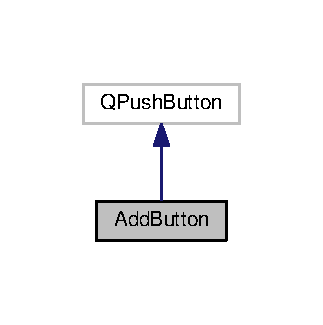
\includegraphics[width=155pt]{class_add_button__inherit__graph}
\end{center}
\end{figure}


Collaboration diagram for Add\+Button\+:
\nopagebreak
\begin{figure}[H]
\begin{center}
\leavevmode
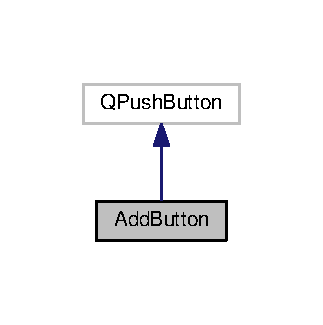
\includegraphics[width=155pt]{class_add_button__coll__graph}
\end{center}
\end{figure}
\subsection*{Public Member Functions}
\begin{DoxyCompactItemize}
\item 
{\bfseries Add\+Button} (Q\+Widget $\ast$parent=0)\hypertarget{class_add_button_a503970bfbab5c9f2d8be45b95f15858e}{}\label{class_add_button_a503970bfbab5c9f2d8be45b95f15858e}

\item 
void {\bfseries mouse\+Press\+Event} (Q\+Mouse\+Event $\ast$event)\hypertarget{class_add_button_ae9cbb131d605755ff68a4d1bd7a47858}{}\label{class_add_button_ae9cbb131d605755ff68a4d1bd7a47858}

\end{DoxyCompactItemize}
\subsection*{Friends}
\begin{DoxyCompactItemize}
\item 
class {\bfseries My\+Scroll\+Area\+Widget}\hypertarget{class_add_button_a96efa7b91da8b371cdcf311988e63048}{}\label{class_add_button_a96efa7b91da8b371cdcf311988e63048}

\item 
class {\bfseries Add\+Button\+\_\+\+Test}\hypertarget{class_add_button_a3a5382161c0a9590f097655075ffe7d4}{}\label{class_add_button_a3a5382161c0a9590f097655075ffe7d4}

\end{DoxyCompactItemize}


The documentation for this class was generated from the following files\+:\begin{DoxyCompactItemize}
\item 
/home/trance/\+L\+T\+Esim/\+Internal.\+L\+T\+Esim\+Generator/\+L\+T\+Esim\+Generator\+G\+U\+I/\+Maps/\+Traffic/\+Map\+Components/addbutton.\+h\item 
/home/trance/\+L\+T\+Esim/\+Internal.\+L\+T\+Esim\+Generator/\+L\+T\+Esim\+Generator\+G\+U\+I/\+Maps/\+Traffic/\+Map\+Components/addbutton.\+cpp\end{DoxyCompactItemize}

\hypertarget{class_add_button___test}{}\section{Add\+Button\+\_\+\+Test Class Reference}
\label{class_add_button___test}\index{Add\+Button\+\_\+\+Test@{Add\+Button\+\_\+\+Test}}


Inheritance diagram for Add\+Button\+\_\+\+Test\+:
\nopagebreak
\begin{figure}[H]
\begin{center}
\leavevmode
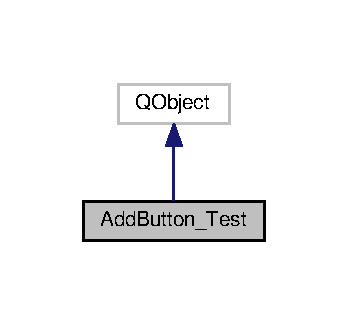
\includegraphics[width=167pt]{class_add_button___test__inherit__graph}
\end{center}
\end{figure}


Collaboration diagram for Add\+Button\+\_\+\+Test\+:
\nopagebreak
\begin{figure}[H]
\begin{center}
\leavevmode
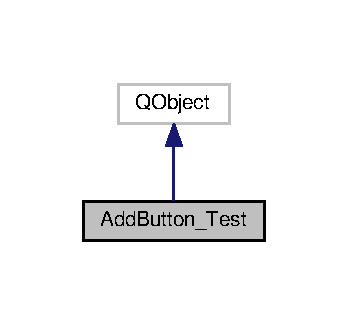
\includegraphics[width=167pt]{class_add_button___test__coll__graph}
\end{center}
\end{figure}


The documentation for this class was generated from the following files\+:\begin{DoxyCompactItemize}
\item 
/home/trance/\+L\+T\+Esim/\+Internal.\+L\+T\+Esim\+Generator/\+L\+T\+Esim\+Generator\+G\+U\+I/\+Maps/\+Traffic/\+Map\+Test/\+Map\+Components\+Test/addbutton\+\_\+test.\+h\item 
/home/trance/\+L\+T\+Esim/\+Internal.\+L\+T\+Esim\+Generator/\+L\+T\+Esim\+Generator\+G\+U\+I/\+Maps/\+Traffic/\+Map\+Test/\+Map\+Components\+Test/addbutton\+\_\+test.\+cpp\end{DoxyCompactItemize}

\hypertarget{class_addftpdl}{}\section{Addftpdl Class Reference}
\label{class_addftpdl}\index{Addftpdl@{Addftpdl}}
\subsection*{Public Member Functions}
\begin{DoxyCompactItemize}
\item 
void {\bfseries set\+Qci} (Q\+String value)\hypertarget{class_addftpdl_aa28113afd1eb26e955ed5cf69270b384}{}\label{class_addftpdl_aa28113afd1eb26e955ed5cf69270b384}

\item 
Q\+String {\bfseries get\+Qci} ()\hypertarget{class_addftpdl_a1cc593949c942ead587cf23ea8640905}{}\label{class_addftpdl_a1cc593949c942ead587cf23ea8640905}

\item 
void {\bfseries set\+Filesize} (Q\+String value)\hypertarget{class_addftpdl_aa593b4122d5eac0d527bc62245d87c31}{}\label{class_addftpdl_aa593b4122d5eac0d527bc62245d87c31}

\item 
Q\+String {\bfseries get\+Filesize} ()\hypertarget{class_addftpdl_a4fe91603ac80d13f0dceeb089a6eab60}{}\label{class_addftpdl_a4fe91603ac80d13f0dceeb089a6eab60}

\item 
void {\bfseries set\+Minthroughput} (Q\+String value)\hypertarget{class_addftpdl_aee3128f9ee8ee9493ee170bb04d0876a}{}\label{class_addftpdl_aee3128f9ee8ee9493ee170bb04d0876a}

\item 
Q\+String {\bfseries get\+Minthroughput} ()\hypertarget{class_addftpdl_a419c7f361db5f9a78dc6ef54657c24b3}{}\label{class_addftpdl_a419c7f361db5f9a78dc6ef54657c24b3}

\end{DoxyCompactItemize}


The documentation for this class was generated from the following files\+:\begin{DoxyCompactItemize}
\item 
/home/trance/\+L\+T\+Esim/\+Internal.\+L\+T\+Esim\+Generator/\+L\+T\+Esim\+Generator\+G\+U\+I/\+Maps/\+Traffic/\+Custom\+Model/addftpdl.\+h\item 
/home/trance/\+L\+T\+Esim/\+Internal.\+L\+T\+Esim\+Generator/\+L\+T\+Esim\+Generator\+G\+U\+I/\+Maps/\+Traffic/\+Custom\+Model/addftpdl.\+cpp\end{DoxyCompactItemize}

\hypertarget{class_add_ftp_dl_form}{}\section{Add\+Ftp\+Dl\+Form Class Reference}
\label{class_add_ftp_dl_form}\index{Add\+Ftp\+Dl\+Form@{Add\+Ftp\+Dl\+Form}}


Inheritance diagram for Add\+Ftp\+Dl\+Form\+:
\nopagebreak
\begin{figure}[H]
\begin{center}
\leavevmode
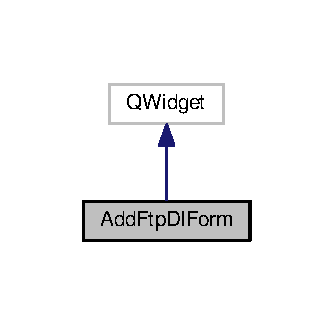
\includegraphics[width=160pt]{class_add_ftp_dl_form__inherit__graph}
\end{center}
\end{figure}


Collaboration diagram for Add\+Ftp\+Dl\+Form\+:
\nopagebreak
\begin{figure}[H]
\begin{center}
\leavevmode
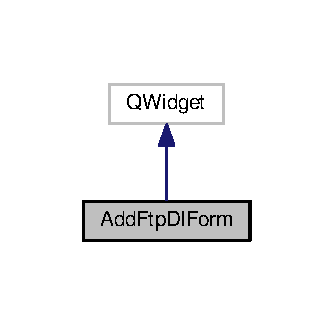
\includegraphics[width=160pt]{class_add_ftp_dl_form__coll__graph}
\end{center}
\end{figure}
\subsection*{Public Member Functions}
\begin{DoxyCompactItemize}
\item 
{\bfseries Add\+Ftp\+Dl\+Form} (Q\+Widget $\ast$parent=0)\hypertarget{class_add_ftp_dl_form_a13734697d4f55222183d448e6788f1ba}{}\label{class_add_ftp_dl_form_a13734697d4f55222183d448e6788f1ba}

\item 
void {\bfseries set\+Parameters} (\hyperlink{class_addftpdl}{Addftpdl} $\ast$addftpdl)\hypertarget{class_add_ftp_dl_form_a0243349a4ba5088cb57c56041c35bf27}{}\label{class_add_ftp_dl_form_a0243349a4ba5088cb57c56041c35bf27}

\item 
void {\bfseries add\+To\+List} ()\hypertarget{class_add_ftp_dl_form_af3bc20e8a30ab6d25b7c477ad017cb81}{}\label{class_add_ftp_dl_form_af3bc20e8a30ab6d25b7c477ad017cb81}

\item 
void {\bfseries check\+File\+Size} ()\hypertarget{class_add_ftp_dl_form_a761b18984d4fe04f02849a283b5af07d}{}\label{class_add_ftp_dl_form_a761b18984d4fe04f02849a283b5af07d}

\end{DoxyCompactItemize}
\subsection*{Public Attributes}
\begin{DoxyCompactItemize}
\item 
Q\+Combo\+Box $\ast$ {\bfseries qci\+Add\+Ftp\+Dl\+Pointer}\hypertarget{class_add_ftp_dl_form_aceb2a15b754c9e5f79099370fb01ec88}{}\label{class_add_ftp_dl_form_aceb2a15b754c9e5f79099370fb01ec88}

\end{DoxyCompactItemize}


The documentation for this class was generated from the following files\+:\begin{DoxyCompactItemize}
\item 
/home/trance/\+L\+T\+Esim/\+Internal.\+L\+T\+Esim\+Generator/\+L\+T\+Esim\+Generator\+G\+U\+I/\+Maps/\+Traffic/\+Custom\+Model/addftpdlform.\+h\item 
/home/trance/\+L\+T\+Esim/\+Internal.\+L\+T\+Esim\+Generator/\+L\+T\+Esim\+Generator\+G\+U\+I/\+Maps/\+Traffic/\+Custom\+Model/addftpdlform.\+cpp\end{DoxyCompactItemize}

\hypertarget{class_addftpul}{}\section{Addftpul Class Reference}
\label{class_addftpul}\index{Addftpul@{Addftpul}}
\subsection*{Public Member Functions}
\begin{DoxyCompactItemize}
\item 
void {\bfseries set\+Qci} (Q\+String value)\hypertarget{class_addftpul_a1e7e4022de1276e4da3448e107bcc4ab}{}\label{class_addftpul_a1e7e4022de1276e4da3448e107bcc4ab}

\item 
Q\+String {\bfseries get\+Qci} ()\hypertarget{class_addftpul_acbdf2d58b27f4e24b33656aaf92bc630}{}\label{class_addftpul_acbdf2d58b27f4e24b33656aaf92bc630}

\item 
void {\bfseries set\+Filesize} (Q\+String value)\hypertarget{class_addftpul_aa1b4996bf303b0a21292f98be1f77c68}{}\label{class_addftpul_aa1b4996bf303b0a21292f98be1f77c68}

\item 
Q\+String {\bfseries get\+Filesize} ()\hypertarget{class_addftpul_aa70abdc1dc21c2b4778efce4e2e529b5}{}\label{class_addftpul_aa70abdc1dc21c2b4778efce4e2e529b5}

\item 
void {\bfseries set\+Minthroughput} (Q\+String value)\hypertarget{class_addftpul_ac768422a8534887ac2abdbe453c9da87}{}\label{class_addftpul_ac768422a8534887ac2abdbe453c9da87}

\item 
Q\+String {\bfseries get\+Minthroughput} ()\hypertarget{class_addftpul_a3dcb2b978a2f5e4136d2ecc1d225c18e}{}\label{class_addftpul_a3dcb2b978a2f5e4136d2ecc1d225c18e}

\end{DoxyCompactItemize}


The documentation for this class was generated from the following files\+:\begin{DoxyCompactItemize}
\item 
/home/trance/\+L\+T\+Esim/\+Internal.\+L\+T\+Esim\+Generator/\+L\+T\+Esim\+Generator\+G\+U\+I/\+Maps/\+Traffic/\+Custom\+Model/addftpul.\+h\item 
/home/trance/\+L\+T\+Esim/\+Internal.\+L\+T\+Esim\+Generator/\+L\+T\+Esim\+Generator\+G\+U\+I/\+Maps/\+Traffic/\+Custom\+Model/addftpul.\+cpp\end{DoxyCompactItemize}

\hypertarget{class_add_ftp_ul_form}{}\section{Add\+Ftp\+Ul\+Form Class Reference}
\label{class_add_ftp_ul_form}\index{Add\+Ftp\+Ul\+Form@{Add\+Ftp\+Ul\+Form}}


Inheritance diagram for Add\+Ftp\+Ul\+Form\+:
\nopagebreak
\begin{figure}[H]
\begin{center}
\leavevmode
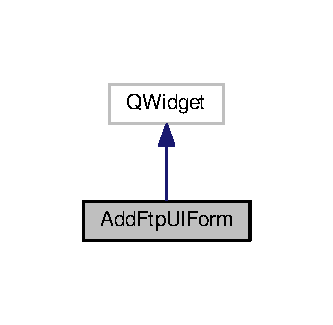
\includegraphics[width=160pt]{class_add_ftp_ul_form__inherit__graph}
\end{center}
\end{figure}


Collaboration diagram for Add\+Ftp\+Ul\+Form\+:
\nopagebreak
\begin{figure}[H]
\begin{center}
\leavevmode
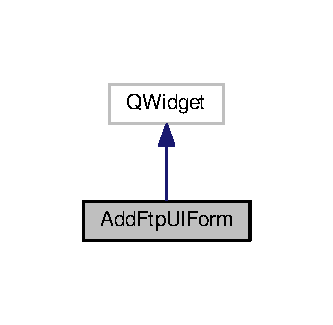
\includegraphics[width=160pt]{class_add_ftp_ul_form__coll__graph}
\end{center}
\end{figure}
\subsection*{Public Member Functions}
\begin{DoxyCompactItemize}
\item 
{\bfseries Add\+Ftp\+Ul\+Form} (Q\+Widget $\ast$parent=0)\hypertarget{class_add_ftp_ul_form_a295bac01a0185361a45a47810dec71a0}{}\label{class_add_ftp_ul_form_a295bac01a0185361a45a47810dec71a0}

\item 
void {\bfseries set\+Parameters} (\hyperlink{class_addftpul}{Addftpul} $\ast$addftpul)\hypertarget{class_add_ftp_ul_form_a59c49d838a8eb78757d444771b0a01f7}{}\label{class_add_ftp_ul_form_a59c49d838a8eb78757d444771b0a01f7}

\item 
void {\bfseries add\+To\+List} ()\hypertarget{class_add_ftp_ul_form_a8a4180aa460ddb2f0130e84f7d3889af}{}\label{class_add_ftp_ul_form_a8a4180aa460ddb2f0130e84f7d3889af}

\item 
void {\bfseries check\+File\+Size} ()\hypertarget{class_add_ftp_ul_form_a110c9a0306bde37ab964d8e2e90a42db}{}\label{class_add_ftp_ul_form_a110c9a0306bde37ab964d8e2e90a42db}

\end{DoxyCompactItemize}
\subsection*{Public Attributes}
\begin{DoxyCompactItemize}
\item 
Q\+Combo\+Box $\ast$ {\bfseries qci\+Add\+Ftp\+Ul\+Pointer}\hypertarget{class_add_ftp_ul_form_a972631cb3318fb58f483d8f79e32047d}{}\label{class_add_ftp_ul_form_a972631cb3318fb58f483d8f79e32047d}

\end{DoxyCompactItemize}


The documentation for this class was generated from the following files\+:\begin{DoxyCompactItemize}
\item 
/home/trance/\+L\+T\+Esim/\+Internal.\+L\+T\+Esim\+Generator/\+L\+T\+Esim\+Generator\+G\+U\+I/\+Maps/\+Traffic/\+Custom\+Model/addftpulform.\+h\item 
/home/trance/\+L\+T\+Esim/\+Internal.\+L\+T\+Esim\+Generator/\+L\+T\+Esim\+Generator\+G\+U\+I/\+Maps/\+Traffic/\+Custom\+Model/addftpulform.\+cpp\end{DoxyCompactItemize}

\hypertarget{class_addping}{}\section{Addping Class Reference}
\label{class_addping}\index{Addping@{Addping}}
\subsection*{Public Member Functions}
\begin{DoxyCompactItemize}
\item 
void {\bfseries set\+Qci} (Q\+String value)\hypertarget{class_addping_ae67680c8f4ceb435dd83cbc887daed45}{}\label{class_addping_ae67680c8f4ceb435dd83cbc887daed45}

\item 
Q\+String {\bfseries get\+Qci} ()\hypertarget{class_addping_af086526de78bc784750135a8ec9ec85d}{}\label{class_addping_af086526de78bc784750135a8ec9ec85d}

\item 
void {\bfseries set\+Number\+Of\+Pings} (Q\+String value)\hypertarget{class_addping_a33dc2e415015e2d04c59e1e522f5eaf9}{}\label{class_addping_a33dc2e415015e2d04c59e1e522f5eaf9}

\item 
Q\+String {\bfseries get\+Number\+Of\+Pings} ()\hypertarget{class_addping_ad1d6a06520a054c64d1926e68d53c355}{}\label{class_addping_ad1d6a06520a054c64d1926e68d53c355}

\item 
void {\bfseries set\+Interval} (Q\+String value)\hypertarget{class_addping_a2ac74755c1ce94dc50121f6fc05d002d}{}\label{class_addping_a2ac74755c1ce94dc50121f6fc05d002d}

\item 
Q\+String {\bfseries get\+Interval} ()\hypertarget{class_addping_ad1ee5a36b855da55214030165ea53490}{}\label{class_addping_ad1ee5a36b855da55214030165ea53490}

\item 
void {\bfseries set\+Min\+Recieved\+Pings} (Q\+String value)\hypertarget{class_addping_aabc3dcb39ff41baa794ef1eddf398dc5}{}\label{class_addping_aabc3dcb39ff41baa794ef1eddf398dc5}

\item 
Q\+String {\bfseries get\+Min\+Recieved\+Pings} ()\hypertarget{class_addping_a685a6c82bef32e4c6f9b15c8413710f0}{}\label{class_addping_a685a6c82bef32e4c6f9b15c8413710f0}

\end{DoxyCompactItemize}


The documentation for this class was generated from the following files\+:\begin{DoxyCompactItemize}
\item 
/home/trance/\+L\+T\+Esim/\+Internal.\+L\+T\+Esim\+Generator/\+L\+T\+Esim\+Generator\+G\+U\+I/\+Maps/\+Traffic/\+Custom\+Model/addping.\+h\item 
/home/trance/\+L\+T\+Esim/\+Internal.\+L\+T\+Esim\+Generator/\+L\+T\+Esim\+Generator\+G\+U\+I/\+Maps/\+Traffic/\+Custom\+Model/addping.\+cpp\end{DoxyCompactItemize}

\hypertarget{class_add_ping_form}{}\section{Add\+Ping\+Form Class Reference}
\label{class_add_ping_form}\index{Add\+Ping\+Form@{Add\+Ping\+Form}}


Inheritance diagram for Add\+Ping\+Form\+:
\nopagebreak
\begin{figure}[H]
\begin{center}
\leavevmode
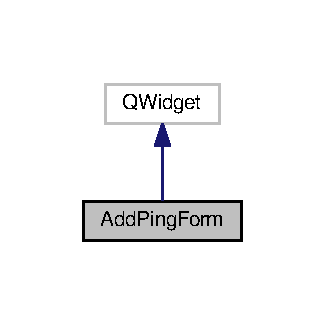
\includegraphics[width=156pt]{class_add_ping_form__inherit__graph}
\end{center}
\end{figure}


Collaboration diagram for Add\+Ping\+Form\+:
\nopagebreak
\begin{figure}[H]
\begin{center}
\leavevmode
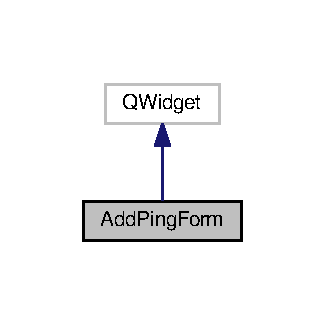
\includegraphics[width=156pt]{class_add_ping_form__coll__graph}
\end{center}
\end{figure}
\subsection*{Public Member Functions}
\begin{DoxyCompactItemize}
\item 
{\bfseries Add\+Ping\+Form} (Q\+Widget $\ast$parent=0)\hypertarget{class_add_ping_form_ab602e336625dcff5c825755db0d5e8b6}{}\label{class_add_ping_form_ab602e336625dcff5c825755db0d5e8b6}

\item 
void {\bfseries set\+Parameters} (\hyperlink{class_addping}{Addping} $\ast$addping)\hypertarget{class_add_ping_form_a7aea79b177eb96abaa8d9521338c5a83}{}\label{class_add_ping_form_a7aea79b177eb96abaa8d9521338c5a83}

\item 
void {\bfseries add\+To\+Ping\+List} ()\hypertarget{class_add_ping_form_ab3ba29ade6646207bdd6f24b93ea01c4}{}\label{class_add_ping_form_ab3ba29ade6646207bdd6f24b93ea01c4}

\end{DoxyCompactItemize}
\subsection*{Public Attributes}
\begin{DoxyCompactItemize}
\item 
Q\+Combo\+Box $\ast$ {\bfseries qci\+Addping\+Pointer}\hypertarget{class_add_ping_form_a6b2787b999e70601336ea0439153c1a5}{}\label{class_add_ping_form_a6b2787b999e70601336ea0439153c1a5}

\end{DoxyCompactItemize}


The documentation for this class was generated from the following files\+:\begin{DoxyCompactItemize}
\item 
/home/trance/\+L\+T\+Esim/\+Internal.\+L\+T\+Esim\+Generator/\+L\+T\+Esim\+Generator\+G\+U\+I/\+Maps/\+Traffic/\+Custom\+Model/addpingform.\+h\item 
/home/trance/\+L\+T\+Esim/\+Internal.\+L\+T\+Esim\+Generator/\+L\+T\+Esim\+Generator\+G\+U\+I/\+Maps/\+Traffic/\+Custom\+Model/addpingform.\+cpp\end{DoxyCompactItemize}

\hypertarget{class_add_project_window}{}\section{Add\+Project\+Window Class Reference}
\label{class_add_project_window}\index{Add\+Project\+Window@{Add\+Project\+Window}}


Inheritance diagram for Add\+Project\+Window\+:
\nopagebreak
\begin{figure}[H]
\begin{center}
\leavevmode
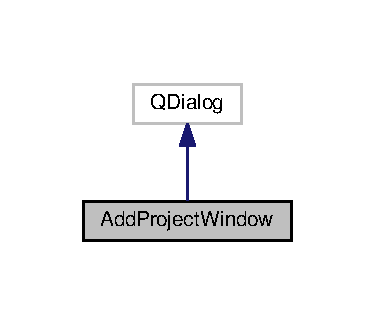
\includegraphics[width=180pt]{class_add_project_window__inherit__graph}
\end{center}
\end{figure}


Collaboration diagram for Add\+Project\+Window\+:
\nopagebreak
\begin{figure}[H]
\begin{center}
\leavevmode
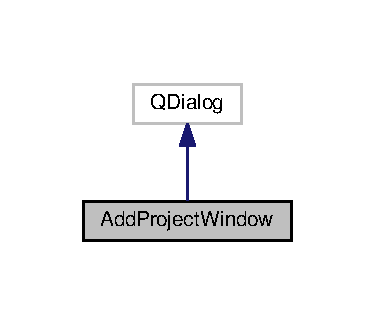
\includegraphics[width=180pt]{class_add_project_window__coll__graph}
\end{center}
\end{figure}
\subsection*{Signals}
\begin{DoxyCompactItemize}
\item 
void {\bfseries create\+New\+Project} (const Q\+String \&project\+Name, const Q\+String \&directory)\hypertarget{class_add_project_window_a547c205329ab94a9b3d7d973e6978030}{}\label{class_add_project_window_a547c205329ab94a9b3d7d973e6978030}

\end{DoxyCompactItemize}
\subsection*{Public Member Functions}
\begin{DoxyCompactItemize}
\item 
{\bfseries Add\+Project\+Window} (Q\+Widget $\ast$parent=0)\hypertarget{class_add_project_window_aa99d418a2a7aba20c9e41535d3d4e9cc}{}\label{class_add_project_window_aa99d418a2a7aba20c9e41535d3d4e9cc}

\item 
void {\bfseries clear\+Input\+Area} ()\hypertarget{class_add_project_window_a0c40ddf9f95f9aca2d6c705cd0edcdbf}{}\label{class_add_project_window_a0c40ddf9f95f9aca2d6c705cd0edcdbf}

\item 
void {\bfseries set\+Default\+Dir} (Q\+String dir)\hypertarget{class_add_project_window_a0c714f31adb731f0100396341bbd7498}{}\label{class_add_project_window_a0c714f31adb731f0100396341bbd7498}

\item 
void {\bfseries set\+App\+Settings} (\hyperlink{class_app_settings}{App\+Settings} $\ast$value)\hypertarget{class_add_project_window_ad4389df3a8c0d9e5172cf53745c3b5c1}{}\label{class_add_project_window_ad4389df3a8c0d9e5172cf53745c3b5c1}

\end{DoxyCompactItemize}


The documentation for this class was generated from the following files\+:\begin{DoxyCompactItemize}
\item 
/home/trance/\+L\+T\+Esim/\+Internal.\+L\+T\+Esim\+Generator/\+L\+T\+Esim\+Generator\+G\+U\+I/\+Management\+Window/\+Add\+Project\+Window/add\+Project\+Window.\+h\item 
/home/trance/\+L\+T\+Esim/\+Internal.\+L\+T\+Esim\+Generator/\+L\+T\+Esim\+Generator\+G\+U\+I/\+Management\+Window/\+Add\+Project\+Window/add\+Project\+Window.\+cpp\end{DoxyCompactItemize}

\hypertarget{class_addservicereq}{}\section{Addservicereq Class Reference}
\label{class_addservicereq}\index{Addservicereq@{Addservicereq}}
\subsection*{Public Member Functions}
\begin{DoxyCompactItemize}
\item 
void {\bfseries set\+Qciarray} (Q\+String value)\hypertarget{class_addservicereq_a9faf4cb46ceadef2ab09689834abb8ab}{}\label{class_addservicereq_a9faf4cb46ceadef2ab09689834abb8ab}

\item 
Q\+String {\bfseries get\+Qciarray} ()\hypertarget{class_addservicereq_a0ec9ab2635ad76520a816e06821d1171}{}\label{class_addservicereq_a0ec9ab2635ad76520a816e06821d1171}

\item 
void {\bfseries set\+Time\+To\+Wait\+For\+Attach} (Q\+String value)\hypertarget{class_addservicereq_a049ec8092ae989d948be6b4f77f68aa2}{}\label{class_addservicereq_a049ec8092ae989d948be6b4f77f68aa2}

\item 
Q\+String {\bfseries get\+Time\+To\+Wait\+For\+Attach} ()\hypertarget{class_addservicereq_a6a4f6882c87747b145eed765b75bde21}{}\label{class_addservicereq_a6a4f6882c87747b145eed765b75bde21}

\item 
void {\bfseries set\+Interval\+Between\+Ul\+Data} (Q\+String value)\hypertarget{class_addservicereq_a3f461ef967f7225d24d577865559a35b}{}\label{class_addservicereq_a3f461ef967f7225d24d577865559a35b}

\item 
Q\+String {\bfseries get\+Interval\+Between\+Ul\+Data} ()\hypertarget{class_addservicereq_a7b7d70d7871b269a24905b82de14f8c4}{}\label{class_addservicereq_a7b7d70d7871b269a24905b82de14f8c4}

\end{DoxyCompactItemize}


The documentation for this class was generated from the following files\+:\begin{DoxyCompactItemize}
\item 
/home/trance/\+L\+T\+Esim/\+Internal.\+L\+T\+Esim\+Generator/\+L\+T\+Esim\+Generator\+G\+U\+I/\+Maps/\+Traffic/\+Custom\+Model/addservicereq.\+h\item 
/home/trance/\+L\+T\+Esim/\+Internal.\+L\+T\+Esim\+Generator/\+L\+T\+Esim\+Generator\+G\+U\+I/\+Maps/\+Traffic/\+Custom\+Model/addservicereq.\+cpp\end{DoxyCompactItemize}

\hypertarget{class_add_service_req_form}{}\section{Add\+Service\+Req\+Form Class Reference}
\label{class_add_service_req_form}\index{Add\+Service\+Req\+Form@{Add\+Service\+Req\+Form}}


Inheritance diagram for Add\+Service\+Req\+Form\+:
\nopagebreak
\begin{figure}[H]
\begin{center}
\leavevmode
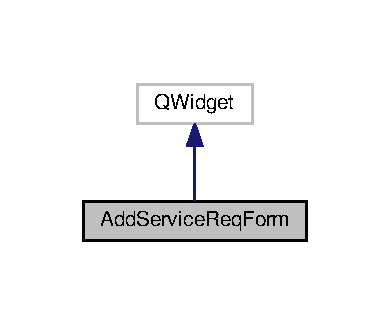
\includegraphics[width=187pt]{class_add_service_req_form__inherit__graph}
\end{center}
\end{figure}


Collaboration diagram for Add\+Service\+Req\+Form\+:
\nopagebreak
\begin{figure}[H]
\begin{center}
\leavevmode
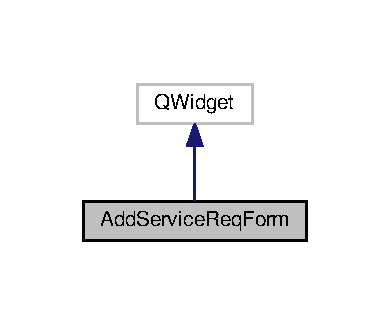
\includegraphics[width=187pt]{class_add_service_req_form__coll__graph}
\end{center}
\end{figure}
\subsection*{Public Member Functions}
\begin{DoxyCompactItemize}
\item 
{\bfseries Add\+Service\+Req\+Form} (Q\+Widget $\ast$parent=0)\hypertarget{class_add_service_req_form_a0cfccd55795702e71dcd0d4b4893f345}{}\label{class_add_service_req_form_a0cfccd55795702e71dcd0d4b4893f345}

\item 
void {\bfseries set\+Parameters} (\hyperlink{class_addservicereq}{Addservicereq} $\ast$addservicereq)\hypertarget{class_add_service_req_form_ac78b1e7887494dc5f3f8e9fbc8097cf1}{}\label{class_add_service_req_form_ac78b1e7887494dc5f3f8e9fbc8097cf1}

\item 
void {\bfseries add\+To\+List} ()\hypertarget{class_add_service_req_form_a25e237b83dd4b9b8e05ada6804048bdb}{}\label{class_add_service_req_form_a25e237b83dd4b9b8e05ada6804048bdb}

\item 
void {\bfseries qci\+Add\+To\+List} ()\hypertarget{class_add_service_req_form_a2133f062f4e58f37cfa626433438b447}{}\label{class_add_service_req_form_a2133f062f4e58f37cfa626433438b447}

\end{DoxyCompactItemize}
\subsection*{Public Attributes}
\begin{DoxyCompactItemize}
\item 
Q\+Combo\+Box $\ast$ {\bfseries qci\+Add\+Service\+Req\+Qci1}\hypertarget{class_add_service_req_form_a0137e65cbf8a871d3bb7e8ba3b030cfe}{}\label{class_add_service_req_form_a0137e65cbf8a871d3bb7e8ba3b030cfe}

\item 
Q\+Combo\+Box $\ast$ {\bfseries qci\+Add\+Service\+Req\+Qci2}\hypertarget{class_add_service_req_form_a462af24d1edb52fb045df4f9c74fc77f}{}\label{class_add_service_req_form_a462af24d1edb52fb045df4f9c74fc77f}

\item 
Q\+Combo\+Box $\ast$ {\bfseries qci\+Add\+Service\+Req\+Qci3}\hypertarget{class_add_service_req_form_a9ac039ae453bab7073d55eac8a131206}{}\label{class_add_service_req_form_a9ac039ae453bab7073d55eac8a131206}

\item 
Q\+Combo\+Box $\ast$ {\bfseries qci\+Add\+Service\+Req\+Qci4}\hypertarget{class_add_service_req_form_ae1f2b58fc96d7a415b7b1360ee616c58}{}\label{class_add_service_req_form_ae1f2b58fc96d7a415b7b1360ee616c58}

\item 
Q\+Combo\+Box $\ast$ {\bfseries qci\+Add\+Service\+Req\+Qci5}\hypertarget{class_add_service_req_form_abe445ce7a3748ed380e4f7df63204fef}{}\label{class_add_service_req_form_abe445ce7a3748ed380e4f7df63204fef}

\item 
Q\+Combo\+Box $\ast$ {\bfseries qci\+Add\+Service\+Req\+Qci6}\hypertarget{class_add_service_req_form_aa9eeb01b170d3f81296acd3673a53aa2}{}\label{class_add_service_req_form_aa9eeb01b170d3f81296acd3673a53aa2}

\item 
Q\+Combo\+Box $\ast$ {\bfseries qci\+Add\+Service\+Req\+Qci7}\hypertarget{class_add_service_req_form_a5ea42ea6cc7cefbe96abbd768b6e44a1}{}\label{class_add_service_req_form_a5ea42ea6cc7cefbe96abbd768b6e44a1}

\item 
Q\+Combo\+Box $\ast$ {\bfseries qci\+Add\+Service\+Req\+Qci8}\hypertarget{class_add_service_req_form_a22faaf5f0fe4b5484d96e0465718cc29}{}\label{class_add_service_req_form_a22faaf5f0fe4b5484d96e0465718cc29}

\item 
Q\+Combo\+Box $\ast$ {\bfseries qci\+Add\+Service\+Req\+Qci9}\hypertarget{class_add_service_req_form_a045040969603dd011e0d99ad066ab8e9}{}\label{class_add_service_req_form_a045040969603dd011e0d99ad066ab8e9}

\end{DoxyCompactItemize}


The documentation for this class was generated from the following files\+:\begin{DoxyCompactItemize}
\item 
/home/trance/\+L\+T\+Esim/\+Internal.\+L\+T\+Esim\+Generator/\+L\+T\+Esim\+Generator\+G\+U\+I/\+Maps/\+Traffic/\+Custom\+Model/addservicereqform.\+h\item 
/home/trance/\+L\+T\+Esim/\+Internal.\+L\+T\+Esim\+Generator/\+L\+T\+Esim\+Generator\+G\+U\+I/\+Maps/\+Traffic/\+Custom\+Model/addservicereqform.\+cpp\end{DoxyCompactItemize}

\hypertarget{class_addstreamdl}{}\section{Addstreamdl Class Reference}
\label{class_addstreamdl}\index{Addstreamdl@{Addstreamdl}}
\subsection*{Public Member Functions}
\begin{DoxyCompactItemize}
\item 
void {\bfseries set\+Qci} (Q\+String value)\hypertarget{class_addstreamdl_a10cdf6f0f575416427bd7023486bad97}{}\label{class_addstreamdl_a10cdf6f0f575416427bd7023486bad97}

\item 
Q\+String {\bfseries get\+Qci} ()\hypertarget{class_addstreamdl_a450587cbc6e5b655650bda27f9f51f68}{}\label{class_addstreamdl_a450587cbc6e5b655650bda27f9f51f68}

\item 
void {\bfseries set\+Speed} (Q\+String value)\hypertarget{class_addstreamdl_a4cf962054bc8f27ac28cbc8717d67c7c}{}\label{class_addstreamdl_a4cf962054bc8f27ac28cbc8717d67c7c}

\item 
Q\+String {\bfseries get\+Speed} ()\hypertarget{class_addstreamdl_a423eb7a4df392bd7dc253eeaa142f2fa}{}\label{class_addstreamdl_a423eb7a4df392bd7dc253eeaa142f2fa}

\item 
void {\bfseries set\+Duration} (Q\+String value)\hypertarget{class_addstreamdl_a07b27450cd06753bcf7f1922f3cbef50}{}\label{class_addstreamdl_a07b27450cd06753bcf7f1922f3cbef50}

\item 
Q\+String {\bfseries get\+Duration} ()\hypertarget{class_addstreamdl_a2b6ebb517d93e6372e9467bf8a649c64}{}\label{class_addstreamdl_a2b6ebb517d93e6372e9467bf8a649c64}

\item 
void {\bfseries set\+Min\+Throughput} (Q\+String value)\hypertarget{class_addstreamdl_a245b85e397bf4f9e05f4c018d836af44}{}\label{class_addstreamdl_a245b85e397bf4f9e05f4c018d836af44}

\item 
Q\+String {\bfseries get\+Min\+Throughput} ()\hypertarget{class_addstreamdl_a71bf1e866cc6ead01ebafb90a4f37f54}{}\label{class_addstreamdl_a71bf1e866cc6ead01ebafb90a4f37f54}

\end{DoxyCompactItemize}


The documentation for this class was generated from the following files\+:\begin{DoxyCompactItemize}
\item 
/home/trance/\+L\+T\+Esim/\+Internal.\+L\+T\+Esim\+Generator/\+L\+T\+Esim\+Generator\+G\+U\+I/\+Maps/\+Traffic/\+Custom\+Model/addstreamdl.\+h\item 
/home/trance/\+L\+T\+Esim/\+Internal.\+L\+T\+Esim\+Generator/\+L\+T\+Esim\+Generator\+G\+U\+I/\+Maps/\+Traffic/\+Custom\+Model/addstreamdl.\+cpp\end{DoxyCompactItemize}

\hypertarget{class_add_stream_dl_form}{}\section{Add\+Stream\+Dl\+Form Class Reference}
\label{class_add_stream_dl_form}\index{Add\+Stream\+Dl\+Form@{Add\+Stream\+Dl\+Form}}


Inheritance diagram for Add\+Stream\+Dl\+Form\+:
\nopagebreak
\begin{figure}[H]
\begin{center}
\leavevmode
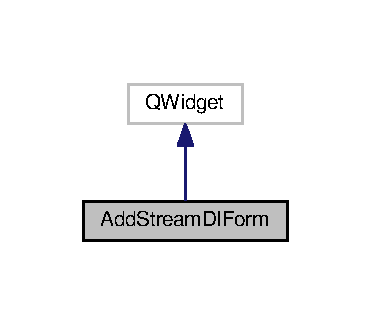
\includegraphics[width=178pt]{class_add_stream_dl_form__inherit__graph}
\end{center}
\end{figure}


Collaboration diagram for Add\+Stream\+Dl\+Form\+:
\nopagebreak
\begin{figure}[H]
\begin{center}
\leavevmode
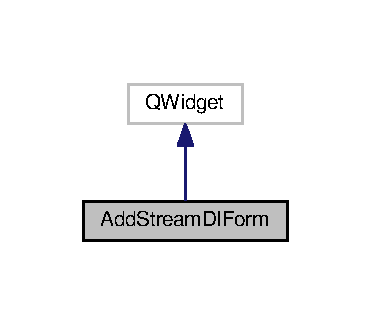
\includegraphics[width=178pt]{class_add_stream_dl_form__coll__graph}
\end{center}
\end{figure}
\subsection*{Public Member Functions}
\begin{DoxyCompactItemize}
\item 
{\bfseries Add\+Stream\+Dl\+Form} (Q\+Widget $\ast$parent=0)\hypertarget{class_add_stream_dl_form_afa2a85a80f61b04969d082ffef72b9f1}{}\label{class_add_stream_dl_form_afa2a85a80f61b04969d082ffef72b9f1}

\item 
void {\bfseries set\+Parameters} (\hyperlink{class_addstreamdl}{Addstreamdl} $\ast$addstreamdl)\hypertarget{class_add_stream_dl_form_a182d398de3c7aa2993fc536286c7623b}{}\label{class_add_stream_dl_form_a182d398de3c7aa2993fc536286c7623b}

\item 
void {\bfseries add\+To\+List} ()\hypertarget{class_add_stream_dl_form_a15cc2397367ff0fca3631b2c558a7ff7}{}\label{class_add_stream_dl_form_a15cc2397367ff0fca3631b2c558a7ff7}

\end{DoxyCompactItemize}
\subsection*{Public Attributes}
\begin{DoxyCompactItemize}
\item 
Q\+Combo\+Box $\ast$ {\bfseries qci\+Add\+Stream\+Dl\+Pointer}\hypertarget{class_add_stream_dl_form_a8820b6721a1a8f0790085c0fade5421a}{}\label{class_add_stream_dl_form_a8820b6721a1a8f0790085c0fade5421a}

\end{DoxyCompactItemize}


The documentation for this class was generated from the following files\+:\begin{DoxyCompactItemize}
\item 
/home/trance/\+L\+T\+Esim/\+Internal.\+L\+T\+Esim\+Generator/\+L\+T\+Esim\+Generator\+G\+U\+I/\+Maps/\+Traffic/\+Custom\+Model/addstreamdlform.\+h\item 
/home/trance/\+L\+T\+Esim/\+Internal.\+L\+T\+Esim\+Generator/\+L\+T\+Esim\+Generator\+G\+U\+I/\+Maps/\+Traffic/\+Custom\+Model/addstreamdlform.\+cpp\end{DoxyCompactItemize}

\hypertarget{class_addstreamul}{}\section{Addstreamul Class Reference}
\label{class_addstreamul}\index{Addstreamul@{Addstreamul}}
\subsection*{Public Member Functions}
\begin{DoxyCompactItemize}
\item 
void {\bfseries set\+Qci} (Q\+String value)\hypertarget{class_addstreamul_a8ac1ba6563353185e5dad1d537468536}{}\label{class_addstreamul_a8ac1ba6563353185e5dad1d537468536}

\item 
Q\+String {\bfseries get\+Qci} ()\hypertarget{class_addstreamul_aacf7152b96fd11bf9accab8c2037c0fc}{}\label{class_addstreamul_aacf7152b96fd11bf9accab8c2037c0fc}

\item 
void {\bfseries set\+Speed} (Q\+String value)\hypertarget{class_addstreamul_a2a3cc8036d59a0c5d5b8775c906968d3}{}\label{class_addstreamul_a2a3cc8036d59a0c5d5b8775c906968d3}

\item 
Q\+String {\bfseries get\+Speed} ()\hypertarget{class_addstreamul_ac45295c633f07e5ca432642e4f7dd21f}{}\label{class_addstreamul_ac45295c633f07e5ca432642e4f7dd21f}

\item 
void {\bfseries set\+Duration} (Q\+String value)\hypertarget{class_addstreamul_a6e3606c586811c962ea8d3735c1ff0af}{}\label{class_addstreamul_a6e3606c586811c962ea8d3735c1ff0af}

\item 
Q\+String {\bfseries get\+Duration} ()\hypertarget{class_addstreamul_a5bd4971f97a32b40578147758d6fbcbf}{}\label{class_addstreamul_a5bd4971f97a32b40578147758d6fbcbf}

\item 
void {\bfseries set\+Min\+Throughput} (Q\+String value)\hypertarget{class_addstreamul_a8288be0b9ac0ef0d0148253d98da173d}{}\label{class_addstreamul_a8288be0b9ac0ef0d0148253d98da173d}

\item 
Q\+String {\bfseries get\+Min\+Throughput} ()\hypertarget{class_addstreamul_ab6c7dfa9c4258b1161637108629b350e}{}\label{class_addstreamul_ab6c7dfa9c4258b1161637108629b350e}

\end{DoxyCompactItemize}


The documentation for this class was generated from the following files\+:\begin{DoxyCompactItemize}
\item 
/home/trance/\+L\+T\+Esim/\+Internal.\+L\+T\+Esim\+Generator/\+L\+T\+Esim\+Generator\+G\+U\+I/\+Maps/\+Traffic/\+Custom\+Model/addstreamul.\+h\item 
/home/trance/\+L\+T\+Esim/\+Internal.\+L\+T\+Esim\+Generator/\+L\+T\+Esim\+Generator\+G\+U\+I/\+Maps/\+Traffic/\+Custom\+Model/addstreamul.\+cpp\end{DoxyCompactItemize}

\hypertarget{class_add_stream_ul_form}{}\section{Add\+Stream\+Ul\+Form Class Reference}
\label{class_add_stream_ul_form}\index{Add\+Stream\+Ul\+Form@{Add\+Stream\+Ul\+Form}}


Inheritance diagram for Add\+Stream\+Ul\+Form\+:
\nopagebreak
\begin{figure}[H]
\begin{center}
\leavevmode
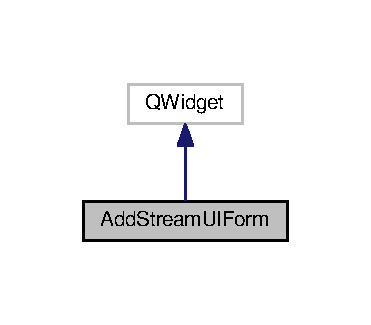
\includegraphics[width=178pt]{class_add_stream_ul_form__inherit__graph}
\end{center}
\end{figure}


Collaboration diagram for Add\+Stream\+Ul\+Form\+:
\nopagebreak
\begin{figure}[H]
\begin{center}
\leavevmode
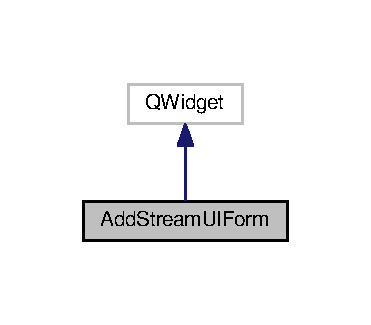
\includegraphics[width=178pt]{class_add_stream_ul_form__coll__graph}
\end{center}
\end{figure}
\subsection*{Public Member Functions}
\begin{DoxyCompactItemize}
\item 
{\bfseries Add\+Stream\+Ul\+Form} (Q\+Widget $\ast$parent=0)\hypertarget{class_add_stream_ul_form_ac6ff3e6edb9919bd1f3c354caee371d7}{}\label{class_add_stream_ul_form_ac6ff3e6edb9919bd1f3c354caee371d7}

\item 
void {\bfseries set\+Parameters} (\hyperlink{class_addstreamul}{Addstreamul} $\ast$addstreamul)\hypertarget{class_add_stream_ul_form_a9310c3ac793231fa3b1e55c28bf727ea}{}\label{class_add_stream_ul_form_a9310c3ac793231fa3b1e55c28bf727ea}

\item 
void {\bfseries add\+To\+List} ()\hypertarget{class_add_stream_ul_form_a646161aaf47baf44fe186ec9b211d2c0}{}\label{class_add_stream_ul_form_a646161aaf47baf44fe186ec9b211d2c0}

\end{DoxyCompactItemize}
\subsection*{Public Attributes}
\begin{DoxyCompactItemize}
\item 
Q\+Combo\+Box $\ast$ {\bfseries qci\+Add\+Stream\+Ul\+Pointer}\hypertarget{class_add_stream_ul_form_ab429b43b14ef862b4c29bc13a872021a}{}\label{class_add_stream_ul_form_ab429b43b14ef862b4c29bc13a872021a}

\end{DoxyCompactItemize}


The documentation for this class was generated from the following files\+:\begin{DoxyCompactItemize}
\item 
/home/trance/\+L\+T\+Esim/\+Internal.\+L\+T\+Esim\+Generator/\+L\+T\+Esim\+Generator\+G\+U\+I/\+Maps/\+Traffic/\+Custom\+Model/addstreamulform.\+h\item 
/home/trance/\+L\+T\+Esim/\+Internal.\+L\+T\+Esim\+Generator/\+L\+T\+Esim\+Generator\+G\+U\+I/\+Maps/\+Traffic/\+Custom\+Model/addstreamulform.\+cpp\end{DoxyCompactItemize}

\hypertarget{class_addsyncedping}{}\section{Addsyncedping Class Reference}
\label{class_addsyncedping}\index{Addsyncedping@{Addsyncedping}}
\subsection*{Public Member Functions}
\begin{DoxyCompactItemize}
\item 
void {\bfseries set\+Qciarray} (Q\+String value)\hypertarget{class_addsyncedping_a5b389118af6eca8e4083b6d8a6da97c5}{}\label{class_addsyncedping_a5b389118af6eca8e4083b6d8a6da97c5}

\item 
Q\+String {\bfseries get\+Qciarray} ()\hypertarget{class_addsyncedping_ac48015c9fa95122d800de516107c37c1}{}\label{class_addsyncedping_ac48015c9fa95122d800de516107c37c1}

\item 
void {\bfseries set\+Time\+Between\+Tasks} (Q\+String value)\hypertarget{class_addsyncedping_af0d50a7354d7f3cf690f3b8b93911a9d}{}\label{class_addsyncedping_af0d50a7354d7f3cf690f3b8b93911a9d}

\item 
Q\+String {\bfseries get\+Time\+Between\+Tasks} ()\hypertarget{class_addsyncedping_a5b1c80801c5236cad77f38578897bd80}{}\label{class_addsyncedping_a5b1c80801c5236cad77f38578897bd80}

\item 
void {\bfseries set\+Number\+Of\+Pings} (Q\+String value)\hypertarget{class_addsyncedping_a0f44a47c8d7c51b2a3576a0d05a07c62}{}\label{class_addsyncedping_a0f44a47c8d7c51b2a3576a0d05a07c62}

\item 
Q\+String {\bfseries get\+Number\+Of\+Pings} ()\hypertarget{class_addsyncedping_ae1abdb02160424820625cde3788b0907}{}\label{class_addsyncedping_ae1abdb02160424820625cde3788b0907}

\item 
void {\bfseries set\+Interval} (Q\+String value)\hypertarget{class_addsyncedping_a342e8e1037356fba744909dd6ef567ba}{}\label{class_addsyncedping_a342e8e1037356fba744909dd6ef567ba}

\item 
Q\+String {\bfseries get\+Interval} ()\hypertarget{class_addsyncedping_aace042931436f9efdf571be7c75e9177}{}\label{class_addsyncedping_aace042931436f9efdf571be7c75e9177}

\item 
void {\bfseries set\+Min\+Received\+Pings} (Q\+String value)\hypertarget{class_addsyncedping_a3194c506769328812f6a28a920455fe7}{}\label{class_addsyncedping_a3194c506769328812f6a28a920455fe7}

\item 
Q\+String {\bfseries get\+Min\+Received\+Pings} ()\hypertarget{class_addsyncedping_a1bf7863bcb311113757bad5317d88963}{}\label{class_addsyncedping_a1bf7863bcb311113757bad5317d88963}

\end{DoxyCompactItemize}


The documentation for this class was generated from the following files\+:\begin{DoxyCompactItemize}
\item 
/home/trance/\+L\+T\+Esim/\+Internal.\+L\+T\+Esim\+Generator/\+L\+T\+Esim\+Generator\+G\+U\+I/\+Maps/\+Traffic/\+Custom\+Model/addsyncedping.\+h\item 
/home/trance/\+L\+T\+Esim/\+Internal.\+L\+T\+Esim\+Generator/\+L\+T\+Esim\+Generator\+G\+U\+I/\+Maps/\+Traffic/\+Custom\+Model/addsyncedping.\+cpp\end{DoxyCompactItemize}

\hypertarget{class_add_synced_ping_form}{}\section{Add\+Synced\+Ping\+Form Class Reference}
\label{class_add_synced_ping_form}\index{Add\+Synced\+Ping\+Form@{Add\+Synced\+Ping\+Form}}


Inheritance diagram for Add\+Synced\+Ping\+Form\+:
\nopagebreak
\begin{figure}[H]
\begin{center}
\leavevmode
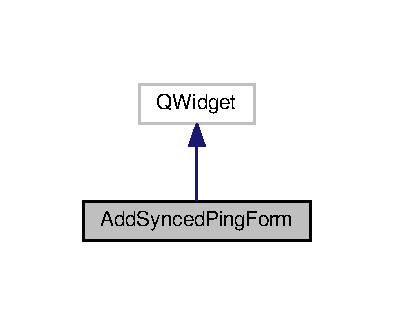
\includegraphics[width=189pt]{class_add_synced_ping_form__inherit__graph}
\end{center}
\end{figure}


Collaboration diagram for Add\+Synced\+Ping\+Form\+:
\nopagebreak
\begin{figure}[H]
\begin{center}
\leavevmode
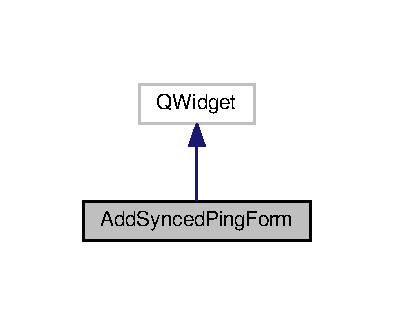
\includegraphics[width=189pt]{class_add_synced_ping_form__coll__graph}
\end{center}
\end{figure}
\subsection*{Public Member Functions}
\begin{DoxyCompactItemize}
\item 
{\bfseries Add\+Synced\+Ping\+Form} (Q\+Widget $\ast$parent=0)\hypertarget{class_add_synced_ping_form_a36047370b1fc7b046347336813fa77a1}{}\label{class_add_synced_ping_form_a36047370b1fc7b046347336813fa77a1}

\item 
void {\bfseries set\+Parameters} (\hyperlink{class_addsyncedping}{Addsyncedping} $\ast$addsyncedping)\hypertarget{class_add_synced_ping_form_a7b200bbaa3aa72010ae2cd728ca97614}{}\label{class_add_synced_ping_form_a7b200bbaa3aa72010ae2cd728ca97614}

\item 
void {\bfseries add\+To\+List} ()\hypertarget{class_add_synced_ping_form_ab40ee058786404ed1110a1fbbf63aeac}{}\label{class_add_synced_ping_form_ab40ee058786404ed1110a1fbbf63aeac}

\item 
void {\bfseries qci\+Add\+To\+List} ()\hypertarget{class_add_synced_ping_form_a21fa236de271d7f3cf6e77829d8614a6}{}\label{class_add_synced_ping_form_a21fa236de271d7f3cf6e77829d8614a6}

\end{DoxyCompactItemize}
\subsection*{Public Attributes}
\begin{DoxyCompactItemize}
\item 
Q\+Combo\+Box $\ast$ {\bfseries qci\+Add\+Synced\+Ping\+Qci1}\hypertarget{class_add_synced_ping_form_afbaf4c5787a4a4ebdbb6f407c1c88512}{}\label{class_add_synced_ping_form_afbaf4c5787a4a4ebdbb6f407c1c88512}

\item 
Q\+Combo\+Box $\ast$ {\bfseries qci\+Add\+Synced\+Ping\+Qci2}\hypertarget{class_add_synced_ping_form_a006eca3a90690fdaf28118df20a17047}{}\label{class_add_synced_ping_form_a006eca3a90690fdaf28118df20a17047}

\item 
Q\+Combo\+Box $\ast$ {\bfseries qci\+Add\+Synced\+Ping\+Qci3}\hypertarget{class_add_synced_ping_form_a6d7c88b3ead5e665c8cc95a4416c3445}{}\label{class_add_synced_ping_form_a6d7c88b3ead5e665c8cc95a4416c3445}

\item 
Q\+Combo\+Box $\ast$ {\bfseries qci\+Add\+Synced\+Ping\+Qci4}\hypertarget{class_add_synced_ping_form_a9b9fcc22b02feeda81e3d025dabc904e}{}\label{class_add_synced_ping_form_a9b9fcc22b02feeda81e3d025dabc904e}

\item 
Q\+Combo\+Box $\ast$ {\bfseries qci\+Add\+Synced\+Ping\+Qci5}\hypertarget{class_add_synced_ping_form_a5c7fc0467f49a6231f9d308bca3dc1a9}{}\label{class_add_synced_ping_form_a5c7fc0467f49a6231f9d308bca3dc1a9}

\item 
Q\+Combo\+Box $\ast$ {\bfseries qci\+Add\+Synced\+Ping\+Qci6}\hypertarget{class_add_synced_ping_form_a39634429f007478a5d7a2f58d38351a7}{}\label{class_add_synced_ping_form_a39634429f007478a5d7a2f58d38351a7}

\item 
Q\+Combo\+Box $\ast$ {\bfseries qci\+Add\+Synced\+Ping\+Qci7}\hypertarget{class_add_synced_ping_form_a88d7ad3bb3b41914109dc40f7ff5259a}{}\label{class_add_synced_ping_form_a88d7ad3bb3b41914109dc40f7ff5259a}

\item 
Q\+Combo\+Box $\ast$ {\bfseries qci\+Add\+Synced\+Ping\+Qci8}\hypertarget{class_add_synced_ping_form_ab9990e723ee95266a03553c4d18e4452}{}\label{class_add_synced_ping_form_ab9990e723ee95266a03553c4d18e4452}

\item 
Q\+Combo\+Box $\ast$ {\bfseries qci\+Add\+Synced\+Ping\+Qci9}\hypertarget{class_add_synced_ping_form_a1dcaa957ecae5e65b3fa331520a9f57f}{}\label{class_add_synced_ping_form_a1dcaa957ecae5e65b3fa331520a9f57f}

\end{DoxyCompactItemize}


The documentation for this class was generated from the following files\+:\begin{DoxyCompactItemize}
\item 
/home/trance/\+L\+T\+Esim/\+Internal.\+L\+T\+Esim\+Generator/\+L\+T\+Esim\+Generator\+G\+U\+I/\+Maps/\+Traffic/\+Custom\+Model/addsyncedpingform.\+h\item 
/home/trance/\+L\+T\+Esim/\+Internal.\+L\+T\+Esim\+Generator/\+L\+T\+Esim\+Generator\+G\+U\+I/\+Maps/\+Traffic/\+Custom\+Model/addsyncedpingform.\+cpp\end{DoxyCompactItemize}

\hypertarget{class_addvoip}{}\section{Addvoip Class Reference}
\label{class_addvoip}\index{Addvoip@{Addvoip}}
\subsection*{Public Member Functions}
\begin{DoxyCompactItemize}
\item 
void {\bfseries set\+Qci} (Q\+String value)\hypertarget{class_addvoip_a0643047c81f40907d065992c8066b3b8}{}\label{class_addvoip_a0643047c81f40907d065992c8066b3b8}

\item 
Q\+String {\bfseries get\+Qci} ()\hypertarget{class_addvoip_a2bca71813ea5f7fc140cc42b5ee5c137}{}\label{class_addvoip_a2bca71813ea5f7fc140cc42b5ee5c137}

\item 
void {\bfseries set\+Duration} (Q\+String value)\hypertarget{class_addvoip_a5977051e0a067af633abf8481de80c10}{}\label{class_addvoip_a5977051e0a067af633abf8481de80c10}

\item 
Q\+String {\bfseries getduration} ()\hypertarget{class_addvoip_a43dc2235f275e3a813617b1a3256533e}{}\label{class_addvoip_a43dc2235f275e3a813617b1a3256533e}

\item 
void {\bfseries set\+Activity\+Factor} (Q\+String value)\hypertarget{class_addvoip_a60dc2494afad5419eadb701a42610419}{}\label{class_addvoip_a60dc2494afad5419eadb701a42610419}

\item 
Q\+String {\bfseries get\+Activity\+Factor} ()\hypertarget{class_addvoip_a595821f64ca873b405a2c8f4915e8309}{}\label{class_addvoip_a595821f64ca873b405a2c8f4915e8309}

\item 
void {\bfseries set\+Max\+Transfer\+Time} (Q\+String value)\hypertarget{class_addvoip_a4cf014cef04cdff47ed49ed6cf126855}{}\label{class_addvoip_a4cf014cef04cdff47ed49ed6cf126855}

\item 
Q\+String {\bfseries get\+Max\+Transfer\+Time} ()\hypertarget{class_addvoip_af6c0b475fdf62c7ef8c8a238e1a9f49a}{}\label{class_addvoip_af6c0b475fdf62c7ef8c8a238e1a9f49a}

\item 
void {\bfseries set\+Min\+Packets\+Received\+In\+Time} (Q\+String value)\hypertarget{class_addvoip_ab8b61130d1f6c4e692ab64b98f6ecc78}{}\label{class_addvoip_ab8b61130d1f6c4e692ab64b98f6ecc78}

\item 
Q\+String {\bfseries get\+Min\+Packets\+Received\+In\+Time} ()\hypertarget{class_addvoip_a8c52e564bafff0dbf278868e20b9003c}{}\label{class_addvoip_a8c52e564bafff0dbf278868e20b9003c}

\end{DoxyCompactItemize}


The documentation for this class was generated from the following files\+:\begin{DoxyCompactItemize}
\item 
/home/trance/\+L\+T\+Esim/\+Internal.\+L\+T\+Esim\+Generator/\+L\+T\+Esim\+Generator\+G\+U\+I/\+Maps/\+Traffic/\+Custom\+Model/addvoip.\+h\item 
/home/trance/\+L\+T\+Esim/\+Internal.\+L\+T\+Esim\+Generator/\+L\+T\+Esim\+Generator\+G\+U\+I/\+Maps/\+Traffic/\+Custom\+Model/addvoip.\+cpp\end{DoxyCompactItemize}

\hypertarget{class_add_voip_form}{}\section{Add\+Voip\+Form Class Reference}
\label{class_add_voip_form}\index{Add\+Voip\+Form@{Add\+Voip\+Form}}


Inheritance diagram for Add\+Voip\+Form\+:
\nopagebreak
\begin{figure}[H]
\begin{center}
\leavevmode
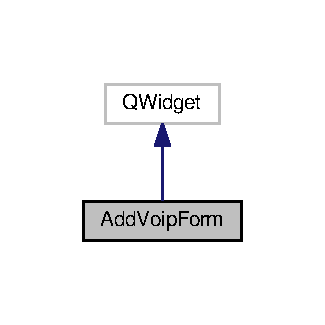
\includegraphics[width=156pt]{class_add_voip_form__inherit__graph}
\end{center}
\end{figure}


Collaboration diagram for Add\+Voip\+Form\+:
\nopagebreak
\begin{figure}[H]
\begin{center}
\leavevmode
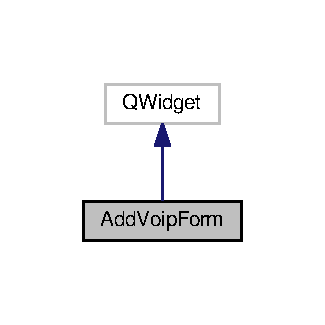
\includegraphics[width=156pt]{class_add_voip_form__coll__graph}
\end{center}
\end{figure}
\subsection*{Public Member Functions}
\begin{DoxyCompactItemize}
\item 
{\bfseries Add\+Voip\+Form} (Q\+Widget $\ast$parent=0)\hypertarget{class_add_voip_form_ae1cd1645ebf965031af269c967901ac2}{}\label{class_add_voip_form_ae1cd1645ebf965031af269c967901ac2}

\item 
void {\bfseries set\+Parameters} (\hyperlink{class_addvoip}{Addvoip} $\ast$addvoip)\hypertarget{class_add_voip_form_a2adfb89905ba253b81c1cf9e3d806ac8}{}\label{class_add_voip_form_a2adfb89905ba253b81c1cf9e3d806ac8}

\item 
void {\bfseries add\+To\+List} ()\hypertarget{class_add_voip_form_ae6da358bab6e81d7c954f6943f5cd019}{}\label{class_add_voip_form_ae6da358bab6e81d7c954f6943f5cd019}

\end{DoxyCompactItemize}
\subsection*{Public Attributes}
\begin{DoxyCompactItemize}
\item 
Q\+Combo\+Box $\ast$ {\bfseries qci\+Add\+Voip\+Pointer}\hypertarget{class_add_voip_form_aa7cf25a54ab44225c209eb96fa6f8299}{}\label{class_add_voip_form_aa7cf25a54ab44225c209eb96fa6f8299}

\end{DoxyCompactItemize}


The documentation for this class was generated from the following files\+:\begin{DoxyCompactItemize}
\item 
/home/trance/\+L\+T\+Esim/\+Internal.\+L\+T\+Esim\+Generator/\+L\+T\+Esim\+Generator\+G\+U\+I/\+Maps/\+Traffic/\+Custom\+Model/addvoipform.\+h\item 
/home/trance/\+L\+T\+Esim/\+Internal.\+L\+T\+Esim\+Generator/\+L\+T\+Esim\+Generator\+G\+U\+I/\+Maps/\+Traffic/\+Custom\+Model/addvoipform.\+cpp\end{DoxyCompactItemize}

\hypertarget{class_app_settings}{}\section{App\+Settings Class Reference}
\label{class_app_settings}\index{App\+Settings@{App\+Settings}}
\subsection*{Public Slots}
\begin{DoxyCompactItemize}
\item 
void {\bfseries create\+New\+Project} (const Q\+String \&project\+Name, const Q\+String \&directory)\hypertarget{class_app_settings_a4758ae8be089a60cd0e52d250d2c9cc6}{}\label{class_app_settings_a4758ae8be089a60cd0e52d250d2c9cc6}

\end{DoxyCompactItemize}
\subsection*{Signals}
\begin{DoxyCompactItemize}
\item 
void {\bfseries current\+Projects} (const std\+::vector$<$ \hyperlink{struct_project}{Project} $>$ \&projects)\hypertarget{class_app_settings_a04473f72a9337a7561c69a617d3e8644}{}\label{class_app_settings_a04473f72a9337a7561c69a617d3e8644}

\end{DoxyCompactItemize}
\subsection*{Public Member Functions}
\begin{DoxyCompactItemize}
\item 
std\+::vector$<$ Q\+List\+Widget\+Item $\ast$ $>$ {\bfseries load\+Settings} ()\hypertarget{class_app_settings_adaf2c6920769fe633bb457817f25e712}{}\label{class_app_settings_adaf2c6920769fe633bb457817f25e712}

\item 
void {\bfseries check\+If\+Exist\+And\+Create\+Settings\+File} ()\hypertarget{class_app_settings_ad43966b109460eec7c4b6966e6beda50}{}\label{class_app_settings_ad43966b109460eec7c4b6966e6beda50}

\item 
void {\bfseries check\+If\+Exist\+And\+Create\+Projects\+File} ()\hypertarget{class_app_settings_a220584efc9258a4a4ce2e7710764cdca}{}\label{class_app_settings_a220584efc9258a4a4ce2e7710764cdca}

\item 
void {\bfseries create\+Project\+Dir\+If\+Not\+Exist} ()\hypertarget{class_app_settings_a61b0424424801e331beff01f6345ddd9}{}\label{class_app_settings_a61b0424424801e331beff01f6345ddd9}

\item 
void {\bfseries read\+Projects\+File} ()\hypertarget{class_app_settings_ae93d08cd7ef4975a4be2f4078dc524af}{}\label{class_app_settings_ae93d08cd7ef4975a4be2f4078dc524af}

\item 
std\+::vector$<$ Q\+List\+Widget\+Item $\ast$ $>$ {\bfseries test\+Projects\+Obtained\+From\+The\+File} ()\hypertarget{class_app_settings_abe01ed44f0d2790df49cd143e5b82331}{}\label{class_app_settings_abe01ed44f0d2790df49cd143e5b82331}

\item 
void {\bfseries traverse\+Projects\+List\+And\+Add\+Project\+If\+Not\+Found} ()\hypertarget{class_app_settings_af3235d6de06a69317c1a97b18ab5636b}{}\label{class_app_settings_af3235d6de06a69317c1a97b18ab5636b}

\item 
void {\bfseries add\+Project} (Q\+List\+Widget\+Item $\ast$new\+\_\+item, Q\+String dir)\hypertarget{class_app_settings_ae4f91140a8f1878e54b0a521821bee68}{}\label{class_app_settings_ae4f91140a8f1878e54b0a521821bee68}

\item 
void {\bfseries remove\+Directory\+Recursively} (Q\+String dir\+\_\+name)\hypertarget{class_app_settings_a3025ec525241da0334a825ebf366a7a1}{}\label{class_app_settings_a3025ec525241da0334a825ebf366a7a1}

\item 
Q\+String {\bfseries get\+Project\+Directory} (const Q\+String \&project\+Name)\hypertarget{class_app_settings_ae1547f13a85eb3d5609fe853e7f0b031}{}\label{class_app_settings_ae1547f13a85eb3d5609fe853e7f0b031}

\item 
void {\bfseries set\+Map\+Type} (const Q\+String \&project\+Name, const Q\+String \&map\+Type)\hypertarget{class_app_settings_ae9acb2ed62bf6e63ee792192e2e2c2f4}{}\label{class_app_settings_ae9acb2ed62bf6e63ee792192e2e2c2f4}

\item 
void {\bfseries write\+\_\+settings\+\_\+file} ()\hypertarget{class_app_settings_a044a33bf439c55642ab876fa3bffdc8b}{}\label{class_app_settings_a044a33bf439c55642ab876fa3bffdc8b}

\item 
void {\bfseries read\+\_\+settings\+\_\+file} ()\hypertarget{class_app_settings_a1b52026abce0b2f22dc8d48ade71dfe3}{}\label{class_app_settings_a1b52026abce0b2f22dc8d48ade71dfe3}

\item 
Q\+String\+List {\bfseries read\+\_\+project\+\_\+file} (Q\+String project\+\_\+name, Q\+String dir)\hypertarget{class_app_settings_a1e9c2d729c124dde43cc53100fa5a8a4}{}\label{class_app_settings_a1e9c2d729c124dde43cc53100fa5a8a4}

\item 
void {\bfseries write\+\_\+project\+\_\+file} (Q\+String project\+\_\+name, Q\+String project\+\_\+content, Q\+String dir)\hypertarget{class_app_settings_a3ff4a29a5a9f052f98bbac4b5f2962c8}{}\label{class_app_settings_a3ff4a29a5a9f052f98bbac4b5f2962c8}

\item 
void {\bfseries write\+\_\+projects\+\_\+file} ()\hypertarget{class_app_settings_a83837d6a6ab4896338b6178637820922}{}\label{class_app_settings_a83837d6a6ab4896338b6178637820922}

\item 
void {\bfseries read\+\_\+projects\+\_\+file} ()\hypertarget{class_app_settings_a20aac1922a43ccbbeeadc3e023bc0ed5}{}\label{class_app_settings_a20aac1922a43ccbbeeadc3e023bc0ed5}

\item 
bool {\bfseries project\+Name\+Taken} (Q\+String project\+Name)\hypertarget{class_app_settings_abc4f77e6834ff97fbf6209426659f03a}{}\label{class_app_settings_abc4f77e6834ff97fbf6209426659f03a}

\item 
bool {\bfseries is\+Project\+Name\+Valid} (const Q\+String \&project\+Name)\hypertarget{class_app_settings_a355deef5b25d7c2566c28d0ebd207c59}{}\label{class_app_settings_a355deef5b25d7c2566c28d0ebd207c59}

\item 
bool {\bfseries is\+Project\+Dir\+Valid} (const Q\+String \&project\+Dir)\hypertarget{class_app_settings_add426453dd17778054607c3142f6e1ac}{}\label{class_app_settings_add426453dd17778054607c3142f6e1ac}

\item 
Q\+String {\bfseries get\+Parameters\+File} () const \hypertarget{class_app_settings_af45425b522c929f2e0d990e9e7a0d9d2}{}\label{class_app_settings_af45425b522c929f2e0d990e9e7a0d9d2}

\item 
void {\bfseries set\+Parameters\+File} (const Q\+String \&value)\hypertarget{class_app_settings_a4ec3658ec7294c3fc446c1bcf2009c61}{}\label{class_app_settings_a4ec3658ec7294c3fc446c1bcf2009c61}

\item 
Q\+String {\bfseries get\+Project\+File} () const \hypertarget{class_app_settings_a349b8265c0ae2a6e5af2929c1b8ec7d5}{}\label{class_app_settings_a349b8265c0ae2a6e5af2929c1b8ec7d5}

\item 
void {\bfseries set\+Project\+File} (const Q\+String \&value)\hypertarget{class_app_settings_a9298dfd433440013467cf47bbf4c36dd}{}\label{class_app_settings_a9298dfd433440013467cf47bbf4c36dd}

\item 
Q\+String {\bfseries get\+Project\+Name} () const \hypertarget{class_app_settings_a533578586b655779b8f7a6d29375b081}{}\label{class_app_settings_a533578586b655779b8f7a6d29375b081}

\item 
void {\bfseries set\+Project\+Name} (const Q\+String \&value)\hypertarget{class_app_settings_ab1567f9a05f3d4a2a800d24d6ae3249e}{}\label{class_app_settings_ab1567f9a05f3d4a2a800d24d6ae3249e}

\item 
Q\+Dir {\bfseries get\+Project\+Dir} () const \hypertarget{class_app_settings_a6e2539bd6bdd0ec38b007e3cff8e891d}{}\label{class_app_settings_a6e2539bd6bdd0ec38b007e3cff8e891d}

\item 
void {\bfseries set\+Project\+Dir} (const Q\+Dir \&value)\hypertarget{class_app_settings_a8f385a5894b950b9687b2f6c551b4eb2}{}\label{class_app_settings_a8f385a5894b950b9687b2f6c551b4eb2}

\item 
Q\+String {\bfseries get\+Default\+New\+Project\+Dir} () const \hypertarget{class_app_settings_a8e09af00975757da8cd520b44db8b4cb}{}\label{class_app_settings_a8e09af00975757da8cd520b44db8b4cb}

\item 
void {\bfseries set\+Default\+New\+Project\+Dir} (const Q\+String \&value)\hypertarget{class_app_settings_a2416714eba17ee60f384cad00124fb9e}{}\label{class_app_settings_a2416714eba17ee60f384cad00124fb9e}

\item 
Q\+String {\bfseries get\+Pro\+File\+Ext} () const \hypertarget{class_app_settings_a540fcd15c9330cc015fab2f43aa79fc1}{}\label{class_app_settings_a540fcd15c9330cc015fab2f43aa79fc1}

\item 
Q\+Dir {\bfseries get\+Project\+\_\+dir} () const \hypertarget{class_app_settings_adc3c9af982f7e368ad741bee099010e0}{}\label{class_app_settings_adc3c9af982f7e368ad741bee099010e0}

\item 
void {\bfseries set\+Project\+\_\+dir} (const Q\+Dir \&value)\hypertarget{class_app_settings_a3060913c5f052852f5a2aa2802351c63}{}\label{class_app_settings_a3060913c5f052852f5a2aa2802351c63}

\item 
Q\+File {\bfseries get\+Projects\+\_\+file} () const \hypertarget{class_app_settings_a5b244cc47342a3a207a4bf855ef5660d}{}\label{class_app_settings_a5b244cc47342a3a207a4bf855ef5660d}

\item 
void {\bfseries set\+Projects\+\_\+file} (const Q\+File \&value)\hypertarget{class_app_settings_a0546a786ddf98f93187d7506e1a14e1c}{}\label{class_app_settings_a0546a786ddf98f93187d7506e1a14e1c}

\item 
Q\+File {\bfseries get\+Settings\+\_\+file} () const \hypertarget{class_app_settings_afe4308305b3178d6fa6f4adc767988a6}{}\label{class_app_settings_afe4308305b3178d6fa6f4adc767988a6}

\item 
void {\bfseries set\+Settings\+\_\+file} (const Q\+File \&value)\hypertarget{class_app_settings_ad793e27d5965a6480da5d6ce17820efe}{}\label{class_app_settings_ad793e27d5965a6480da5d6ce17820efe}

\item 
Q\+String {\bfseries read\+Parameters\+File} ()\hypertarget{class_app_settings_ab59a8b8480c4f02478e4bb67040ba348}{}\label{class_app_settings_ab59a8b8480c4f02478e4bb67040ba348}

\end{DoxyCompactItemize}
\subsection*{Public Attributes}
\begin{DoxyCompactItemize}
\item 
std\+::vector$<$ \hyperlink{struct_project}{Project} $>$ {\bfseries projects}\hypertarget{class_app_settings_a750057357b7231682c87636e0e1c355f}{}\label{class_app_settings_a750057357b7231682c87636e0e1c355f}

\end{DoxyCompactItemize}


The documentation for this class was generated from the following files\+:\begin{DoxyCompactItemize}
\item 
/home/trance/\+L\+T\+Esim/\+Internal.\+L\+T\+Esim\+Generator/\+L\+T\+Esim\+Generator\+G\+U\+I/\+App\+Settings/appsettings.\+h\item 
/home/trance/\+L\+T\+Esim/\+Internal.\+L\+T\+Esim\+Generator/\+L\+T\+Esim\+Generator\+G\+U\+I/\+App\+Settings/appsettings.\+cpp\end{DoxyCompactItemize}

\hypertarget{struct_tuningtraffic_1_1_areas}{}\section{Tuningtraffic\+:\+:Areas Struct Reference}
\label{struct_tuningtraffic_1_1_areas}\index{Tuningtraffic\+::\+Areas@{Tuningtraffic\+::\+Areas}}
\subsection*{Public Attributes}
\begin{DoxyCompactItemize}
\item 
Q\+String {\bfseries area\+\_\+name}\hypertarget{struct_tuningtraffic_1_1_areas_a297675636696c347324da34d6bc2119b}{}\label{struct_tuningtraffic_1_1_areas_a297675636696c347324da34d6bc2119b}

\item 
Q\+String {\bfseries speed}\hypertarget{struct_tuningtraffic_1_1_areas_a64539cfbd72f104932194af33ead762a}{}\label{struct_tuningtraffic_1_1_areas_a64539cfbd72f104932194af33ead762a}

\item 
Q\+String {\bfseries granularity}\hypertarget{struct_tuningtraffic_1_1_areas_a42675f785a229a55b689a3638eb669fa}{}\label{struct_tuningtraffic_1_1_areas_a42675f785a229a55b689a3638eb669fa}

\end{DoxyCompactItemize}


The documentation for this struct was generated from the following file\+:\begin{DoxyCompactItemize}
\item 
/home/trance/\+L\+T\+Esim/\+Internal.\+L\+T\+Esim\+Generator/\+L\+T\+Esim\+Generator\+G\+U\+I/\+Maps/\+Traffic/\+Tuning/tuningtraffic.\+h\end{DoxyCompactItemize}

\hypertarget{class_cell}{}\section{Cell Class Reference}
\label{class_cell}\index{Cell@{Cell}}


Collaboration diagram for Cell\+:
\nopagebreak
\begin{figure}[H]
\begin{center}
\leavevmode
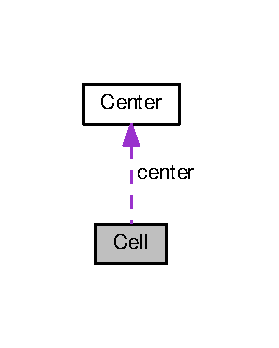
\includegraphics[width=134pt]{class_cell__coll__graph}
\end{center}
\end{figure}
\subsection*{Public Member Functions}
\begin{DoxyCompactItemize}
\item 
{\bfseries Cell} (Q\+String name)\hypertarget{class_cell_a57a2719802c1d23a436ead5ef523264e}{}\label{class_cell_a57a2719802c1d23a436ead5ef523264e}

\item 
Q\+String {\bfseries get\+Cell} ()\hypertarget{class_cell_a7f437e258bd5266d70a01ea2cdf02519}{}\label{class_cell_a7f437e258bd5266d70a01ea2cdf02519}

\item 
Q\+String $\ast$ {\bfseries set\+Params} ()\hypertarget{class_cell_a5124835d0544eea46e8dcfa51fff6e7a}{}\label{class_cell_a5124835d0544eea46e8dcfa51fff6e7a}

\item 
void {\bfseries reset\+Params} ()\hypertarget{class_cell_ad66d2f6034625a2d29f2fb744b0d83aa}{}\label{class_cell_ad66d2f6034625a2d29f2fb744b0d83aa}

\item 
Q\+String {\bfseries get\+Site} ()\hypertarget{class_cell_ac87ee0a1d55763294d14a851d1551124}{}\label{class_cell_ac87ee0a1d55763294d14a851d1551124}

\item 
Q\+String {\bfseries get\+Pci} ()\hypertarget{class_cell_a08e25d5b5b7a6e3af8ab86696436db7a}{}\label{class_cell_a08e25d5b5b7a6e3af8ab86696436db7a}

\item 
Q\+String {\bfseries get\+Position\+\_\+X} ()\hypertarget{class_cell_a78bce141440cc17cc24d4ea639de3dde}{}\label{class_cell_a78bce141440cc17cc24d4ea639de3dde}

\item 
Q\+String {\bfseries get\+Position\+\_\+Y} ()\hypertarget{class_cell_a0f076c847f83c65b01d7973fa779abf5}{}\label{class_cell_a0f076c847f83c65b01d7973fa779abf5}

\item 
Q\+String {\bfseries get\+Earfcn\+Dl} ()\hypertarget{class_cell_a737599f87a3465371ec25bcc0dcc92a4}{}\label{class_cell_a737599f87a3465371ec25bcc0dcc92a4}

\item 
Q\+String {\bfseries get\+Transmit\+Power} ()\hypertarget{class_cell_ac74525d102eafcf0da04c746d70ddb1b}{}\label{class_cell_ac74525d102eafcf0da04c746d70ddb1b}

\item 
Q\+String {\bfseries get\+Ul\+Noise\+And\+Interference} ()\hypertarget{class_cell_a0e3e0ec7480754de2a31590f9c9dc079}{}\label{class_cell_a0e3e0ec7480754de2a31590f9c9dc079}

\item 
void {\bfseries set\+Cell} (Q\+String c)\hypertarget{class_cell_a0a780eaf3218cbee2ded585634a2a0a1}{}\label{class_cell_a0a780eaf3218cbee2ded585634a2a0a1}

\item 
void {\bfseries set\+Site} (Q\+String s)\hypertarget{class_cell_af1fe8b468da9c30f7a134daf9d510212}{}\label{class_cell_af1fe8b468da9c30f7a134daf9d510212}

\item 
void {\bfseries set\+Pci} (Q\+String s)\hypertarget{class_cell_ab72dd0a9fbe24e254e25ea66e4a34c5a}{}\label{class_cell_ab72dd0a9fbe24e254e25ea66e4a34c5a}

\item 
void {\bfseries set\+Position\+\_\+X} (Q\+String px)\hypertarget{class_cell_a9445a38c257ec3e2dc25bff38d9d5948}{}\label{class_cell_a9445a38c257ec3e2dc25bff38d9d5948}

\item 
void {\bfseries set\+Position\+\_\+Y} (Q\+String py)\hypertarget{class_cell_ab688ae364074e0a91744d0e4db64f0a9}{}\label{class_cell_ab688ae364074e0a91744d0e4db64f0a9}

\item 
void {\bfseries set\+Earfcn\+Dl} (Q\+String e)\hypertarget{class_cell_a3e4aca1298f1f45067be89a7e4710a14}{}\label{class_cell_a3e4aca1298f1f45067be89a7e4710a14}

\item 
void {\bfseries set\+Transmit\+Power} (Q\+String t)\hypertarget{class_cell_a12298307ef647d4b4cacfe2efed5214d}{}\label{class_cell_a12298307ef647d4b4cacfe2efed5214d}

\item 
void {\bfseries set\+Ul\+Noise\+And\+Interference} (Q\+String u)\hypertarget{class_cell_a899fe6e29a3160988547ae2bfaf3adfe}{}\label{class_cell_a899fe6e29a3160988547ae2bfaf3adfe}

\item 
Q\+String {\bfseries get\+Cell\+\_\+new\+\_\+name} () const \hypertarget{class_cell_a81b2f4bc74ea50a7c693839f4f024ea4}{}\label{class_cell_a81b2f4bc74ea50a7c693839f4f024ea4}

\item 
void {\bfseries set\+Cell\+\_\+new\+\_\+name} (const Q\+String \&value)\hypertarget{class_cell_af7043367512ea12553c2ed31b1cafe73}{}\label{class_cell_af7043367512ea12553c2ed31b1cafe73}

\item 
bool {\bfseries was\+There\+Changes} ()\hypertarget{class_cell_a75de9576e08b33760b550ce4fed6dd75}{}\label{class_cell_a75de9576e08b33760b550ce4fed6dd75}

\end{DoxyCompactItemize}
\subsection*{Public Attributes}
\begin{DoxyCompactItemize}
\item 
Q\+Check\+Box $\ast$ {\bfseries ch\+Box}\hypertarget{class_cell_a97d2b6ab648a792b85c2276b873ae9e5}{}\label{class_cell_a97d2b6ab648a792b85c2276b873ae9e5}

\item 
\hyperlink{class_center}{Center} $\ast$ {\bfseries center}\hypertarget{class_cell_ab1700f50315b4937b21ebc8518516cd1}{}\label{class_cell_ab1700f50315b4937b21ebc8518516cd1}

\end{DoxyCompactItemize}


The documentation for this class was generated from the following files\+:\begin{DoxyCompactItemize}
\item 
/home/trance/\+L\+T\+Esim/\+Internal.\+L\+T\+Esim\+Generator/\+L\+T\+Esim\+Generator\+G\+U\+I/\+Maps/\+Map\+Objects/cell.\+h\item 
/home/trance/\+L\+T\+Esim/\+Internal.\+L\+T\+Esim\+Generator/\+L\+T\+Esim\+Generator\+G\+U\+I/\+Maps/\+Map\+Objects/cell.\+cpp\end{DoxyCompactItemize}

\hypertarget{class_cell_area}{}\section{Cell\+Area Class Reference}
\label{class_cell_area}\index{Cell\+Area@{Cell\+Area}}


Inheritance diagram for Cell\+Area\+:
\nopagebreak
\begin{figure}[H]
\begin{center}
\leavevmode
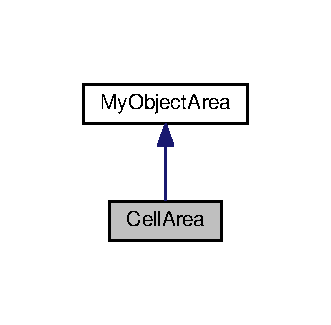
\includegraphics[width=159pt]{class_cell_area__inherit__graph}
\end{center}
\end{figure}


Collaboration diagram for Cell\+Area\+:
\nopagebreak
\begin{figure}[H]
\begin{center}
\leavevmode
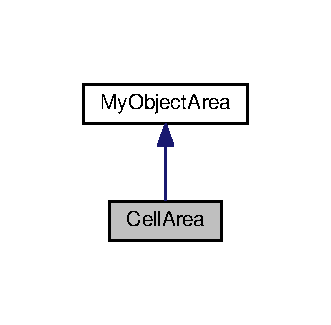
\includegraphics[width=159pt]{class_cell_area__coll__graph}
\end{center}
\end{figure}
\subsection*{Public Member Functions}
\begin{DoxyCompactItemize}
\item 
{\bfseries Cell\+Area} (int positionX, int positionY, Q\+String ID)\hypertarget{class_cell_area_a15484a68caf1bbca21b0c5bf90376c7a}{}\label{class_cell_area_a15484a68caf1bbca21b0c5bf90376c7a}

\item 
bool {\bfseries contain} (int x\+Pos, int y\+Pos, \hyperlink{class_my_object_area}{My\+Object\+Area} $\ast$$\ast$obj\+Ptr1)\hypertarget{class_cell_area_a86f80474e184602d64923eefc39d09a9}{}\label{class_cell_area_a86f80474e184602d64923eefc39d09a9}

\item 
Q\+Point {\bfseries get\+Center} ()\hypertarget{class_cell_area_abca39734a387fa7a9029ea96541a793a}{}\label{class_cell_area_abca39734a387fa7a9029ea96541a793a}

\item 
Q\+String {\bfseries get\+ID} ()\hypertarget{class_cell_area_a506290acadb951c4217cf6828d4eedb2}{}\label{class_cell_area_a506290acadb951c4217cf6828d4eedb2}

\end{DoxyCompactItemize}
\subsection*{Static Public Member Functions}
\begin{DoxyCompactItemize}
\item 
static int {\bfseries getR} ()\hypertarget{class_cell_area_aa28afcd07a265c9bb987d97df5cbe5fa}{}\label{class_cell_area_aa28afcd07a265c9bb987d97df5cbe5fa}

\end{DoxyCompactItemize}
\subsection*{Friends}
\begin{DoxyCompactItemize}
\item 
class {\bfseries Cell\+Area\+\_\+\+Test}\hypertarget{class_cell_area_aa20b890699cb6ef2056c0d229975cb17}{}\label{class_cell_area_aa20b890699cb6ef2056c0d229975cb17}

\end{DoxyCompactItemize}


The documentation for this class was generated from the following files\+:\begin{DoxyCompactItemize}
\item 
/home/trance/\+L\+T\+Esim/\+Internal.\+L\+T\+Esim\+Generator/\+L\+T\+Esim\+Generator\+G\+U\+I/\+Maps/\+Traffic/\+Map\+Components/cellarea.\+h\item 
/home/trance/\+L\+T\+Esim/\+Internal.\+L\+T\+Esim\+Generator/\+L\+T\+Esim\+Generator\+G\+U\+I/\+Maps/\+Traffic/\+Map\+Components/cellarea.\+cpp\end{DoxyCompactItemize}

\hypertarget{class_cell_area___test}{}\section{Cell\+Area\+\_\+\+Test Class Reference}
\label{class_cell_area___test}\index{Cell\+Area\+\_\+\+Test@{Cell\+Area\+\_\+\+Test}}


Inheritance diagram for Cell\+Area\+\_\+\+Test\+:
\nopagebreak
\begin{figure}[H]
\begin{center}
\leavevmode
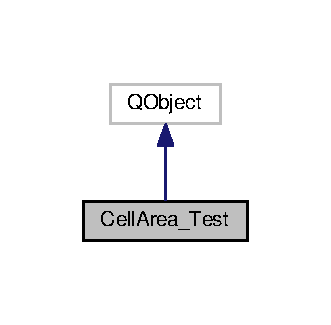
\includegraphics[width=159pt]{class_cell_area___test__inherit__graph}
\end{center}
\end{figure}


Collaboration diagram for Cell\+Area\+\_\+\+Test\+:
\nopagebreak
\begin{figure}[H]
\begin{center}
\leavevmode
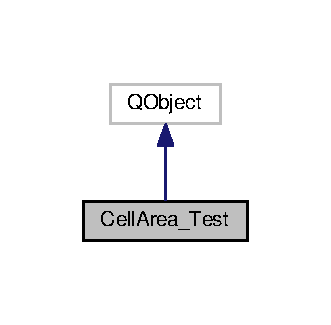
\includegraphics[width=159pt]{class_cell_area___test__coll__graph}
\end{center}
\end{figure}


The documentation for this class was generated from the following files\+:\begin{DoxyCompactItemize}
\item 
/home/trance/\+L\+T\+Esim/\+Internal.\+L\+T\+Esim\+Generator/\+L\+T\+Esim\+Generator\+G\+U\+I/\+Maps/\+Traffic/\+Map\+Test/\+Map\+Components\+Test/cellarea\+\_\+test.\+h\item 
/home/trance/\+L\+T\+Esim/\+Internal.\+L\+T\+Esim\+Generator/\+L\+T\+Esim\+Generator\+G\+U\+I/\+Maps/\+Traffic/\+Map\+Test/\+Map\+Components\+Test/cellarea\+\_\+test.\+cpp\end{DoxyCompactItemize}

\hypertarget{class_cell_data}{}\section{Cell\+Data Class Reference}
\label{class_cell_data}\index{Cell\+Data@{Cell\+Data}}


Inheritance diagram for Cell\+Data\+:
\nopagebreak
\begin{figure}[H]
\begin{center}
\leavevmode
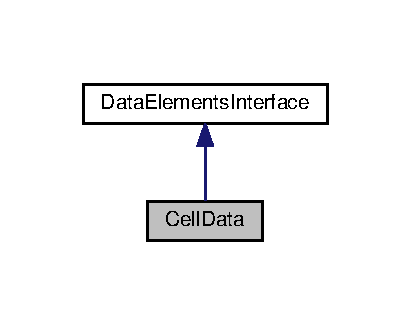
\includegraphics[width=197pt]{class_cell_data__inherit__graph}
\end{center}
\end{figure}


Collaboration diagram for Cell\+Data\+:
\nopagebreak
\begin{figure}[H]
\begin{center}
\leavevmode
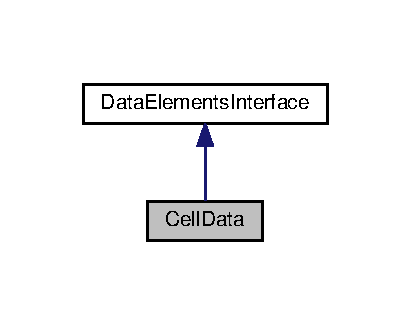
\includegraphics[width=197pt]{class_cell_data__coll__graph}
\end{center}
\end{figure}
\subsection*{Public Member Functions}
\begin{DoxyCompactItemize}
\item 
{\bfseries Cell\+Data} (const Q\+String \&name\+Cell, const Q\+String \&name\+Center, \hyperlink{class_app_settings}{App\+Settings} $\ast$app\+Settings)\hypertarget{class_cell_data_a1187ace2572657fed666a6c5991c9464}{}\label{class_cell_data_a1187ace2572657fed666a6c5991c9464}

\item 
Q\+String {\bfseries get\+Cell\+Name} () const \hypertarget{class_cell_data_ade531de6af31b76efea6bb1cf836318d}{}\label{class_cell_data_ade531de6af31b76efea6bb1cf836318d}

\item 
int {\bfseries get\+Pci} () const \hypertarget{class_cell_data_aca22793b0d73d0e6e052f505244b07c8}{}\label{class_cell_data_aca22793b0d73d0e6e052f505244b07c8}

\item 
int {\bfseries get\+Position\+\_\+X} () const \hypertarget{class_cell_data_acd460d39595e0c940b8a6a0d0f8c043d}{}\label{class_cell_data_acd460d39595e0c940b8a6a0d0f8c043d}

\item 
int {\bfseries get\+Position\+\_\+Y} () const \hypertarget{class_cell_data_aa1488703bc627613d01538d80152ca03}{}\label{class_cell_data_aa1488703bc627613d01538d80152ca03}

\item 
int {\bfseries get\+Earfcn\+Dl} () const \hypertarget{class_cell_data_a759b5347060d91d78f7217f7d80295a4}{}\label{class_cell_data_a759b5347060d91d78f7217f7d80295a4}

\item 
float {\bfseries get\+Transmit\+Power} () const \hypertarget{class_cell_data_a91796a405772ed93ff2629fe75e96c7c}{}\label{class_cell_data_a91796a405772ed93ff2629fe75e96c7c}

\item 
float {\bfseries get\+Ul\+Noise\+And\+Interference} () const \hypertarget{class_cell_data_a467c43df76462ba8ddee25d83c40881d}{}\label{class_cell_data_a467c43df76462ba8ddee25d83c40881d}

\item 
Q\+String {\bfseries get\+Center\+Name} () const \hypertarget{class_cell_data_af6b4d67e3c018bb74c621cc75798d469}{}\label{class_cell_data_af6b4d67e3c018bb74c621cc75798d469}

\item 
int {\bfseries get\+South\+Cell\+Boundary} () const \hypertarget{class_cell_data_a53054ab3fbe627142201c308c7242686}{}\label{class_cell_data_a53054ab3fbe627142201c308c7242686}

\item 
int {\bfseries get\+North\+Cell\+Boundary} () const \hypertarget{class_cell_data_aca10dfb26d07c83c5a7c7823841a0722}{}\label{class_cell_data_aca10dfb26d07c83c5a7c7823841a0722}

\item 
int {\bfseries get\+West\+Cell\+Boundary} () const \hypertarget{class_cell_data_a68a3eb8e440457b00ac4886cdc46e59d}{}\label{class_cell_data_a68a3eb8e440457b00ac4886cdc46e59d}

\item 
int {\bfseries get\+East\+Cell\+Boundary} () const \hypertarget{class_cell_data_a05d3985c904ab7b1143e57038656f4d4}{}\label{class_cell_data_a05d3985c904ab7b1143e57038656f4d4}

\item 
\hyperlink{struct_cell_params}{Cell\+Params} {\bfseries get\+Cell\+Params} () const \hypertarget{class_cell_data_a8af9494e1981a72498079af2e3ec6a76}{}\label{class_cell_data_a8af9494e1981a72498079af2e3ec6a76}

\item 
\hyperlink{struct_center_params}{Center\+Params} {\bfseries get\+Center\+Params} () const \hypertarget{class_cell_data_a98bb4ef815cd67a0eb9fc652145c7c70}{}\label{class_cell_data_a98bb4ef815cd67a0eb9fc652145c7c70}

\item 
void {\bfseries set\+Cell\+Name} (const Q\+String \&cell)\hypertarget{class_cell_data_a196eb66c06727a9698d20fd3992ce35f}{}\label{class_cell_data_a196eb66c06727a9698d20fd3992ce35f}

\item 
void {\bfseries set\+Pci} (int pci)\hypertarget{class_cell_data_a006075b7cf1143243de4fd7bb47ac382}{}\label{class_cell_data_a006075b7cf1143243de4fd7bb47ac382}

\item 
void {\bfseries set\+Position\+\_\+X} (int positionX)\hypertarget{class_cell_data_a10d1a1e312a45184b926e61873d5fb20}{}\label{class_cell_data_a10d1a1e312a45184b926e61873d5fb20}

\item 
void {\bfseries set\+Position\+\_\+Y} (int positionY)\hypertarget{class_cell_data_a0e66ef92e7d772883606330a9b7147cb}{}\label{class_cell_data_a0e66ef92e7d772883606330a9b7147cb}

\item 
void {\bfseries set\+Earfcn\+Dl} (int earfcndl)\hypertarget{class_cell_data_af25ca29aa59f935b8bac39a84dab05a9}{}\label{class_cell_data_af25ca29aa59f935b8bac39a84dab05a9}

\item 
void {\bfseries set\+Transmit\+Power} (float power)\hypertarget{class_cell_data_aa56b0d9abcd8a6578712d0fc758e014b}{}\label{class_cell_data_aa56b0d9abcd8a6578712d0fc758e014b}

\item 
void {\bfseries set\+Ul\+Noise\+And\+Interference} (float ul\+Noise)\hypertarget{class_cell_data_a34d1260736130ed14c598c59608f2785}{}\label{class_cell_data_a34d1260736130ed14c598c59608f2785}

\item 
void {\bfseries set\+Cell\+Params} (const \hyperlink{struct_cell_params}{Cell\+Params} \&params)\hypertarget{class_cell_data_a20935748660ee7cbf7a4cd8740b01c32}{}\label{class_cell_data_a20935748660ee7cbf7a4cd8740b01c32}

\item 
void {\bfseries set\+Center\+Name} (const Q\+String \&center)\hypertarget{class_cell_data_a63b52fe7adb67c5129854384a0a917e8}{}\label{class_cell_data_a63b52fe7adb67c5129854384a0a917e8}

\item 
void {\bfseries set\+South\+Cell\+Boundary} (int south)\hypertarget{class_cell_data_a0976ebf505d907d79f6ae671773320a3}{}\label{class_cell_data_a0976ebf505d907d79f6ae671773320a3}

\item 
void {\bfseries set\+North\+Cell\+Boundary} (int north)\hypertarget{class_cell_data_a1062fc88142921a3d4f6fbb5971f6003}{}\label{class_cell_data_a1062fc88142921a3d4f6fbb5971f6003}

\item 
void {\bfseries set\+West\+Cell\+Boundary} (int west)\hypertarget{class_cell_data_a3d6856eaf2f36a0d3a8bd4cb833ba9c7}{}\label{class_cell_data_a3d6856eaf2f36a0d3a8bd4cb833ba9c7}

\item 
void {\bfseries set\+East\+Cell\+Boundary} (int east)\hypertarget{class_cell_data_a48accedd54bb594f2e1395a9fb33c437}{}\label{class_cell_data_a48accedd54bb594f2e1395a9fb33c437}

\item 
void {\bfseries set\+Center\+Params} (const \hyperlink{struct_center_params}{Center\+Params} \&params)\hypertarget{class_cell_data_a2378088d9091e149d53bee386d6bbd21}{}\label{class_cell_data_a2378088d9091e149d53bee386d6bbd21}

\item 
\hyperlink{struct_cell_params}{Cell\+Params} {\bfseries parse\+Cell\+Data\+From\+List} (Q\+String\+List \&params\+List)\hypertarget{class_cell_data_aca2d037e20f6d87e064e0ceda28cc5d7}{}\label{class_cell_data_aca2d037e20f6d87e064e0ceda28cc5d7}

\item 
\hyperlink{struct_center_params}{Center\+Params} {\bfseries parse\+Center\+Data\+From\+List} (Q\+String\+List \&params\+List)\hypertarget{class_cell_data_af27b75e4cd0fd3112c9b698ee1e45102}{}\label{class_cell_data_af27b75e4cd0fd3112c9b698ee1e45102}

\item 
Q\+String {\bfseries get\+Element\+Type} () const override\hypertarget{class_cell_data_af5b091c26acbc45435a1cb6b509de4d8}{}\label{class_cell_data_af5b091c26acbc45435a1cb6b509de4d8}

\item 
void {\bfseries serialize\+To\+Project\+File} () override\hypertarget{class_cell_data_a4fdbf6bd16db6b0992a304c5d25b91aa}{}\label{class_cell_data_a4fdbf6bd16db6b0992a304c5d25b91aa}

\item 
void {\bfseries serialize\+From\+Project\+File\+Old} (Q\+Byte\+Array raw\+Data) override\hypertarget{class_cell_data_a673847f272bf60e91212f6006c04b5b9}{}\label{class_cell_data_a673847f272bf60e91212f6006c04b5b9}

\item 
void {\bfseries serialize\+From\+Project\+File\+New} (Q\+Dom\+Document xml\+Document) override\hypertarget{class_cell_data_acc97c849d8e379d9eedef17b87daee9b}{}\label{class_cell_data_acc97c849d8e379d9eedef17b87daee9b}

\item 
void {\bfseries serialize\+To\+Script\+Commands} () override\hypertarget{class_cell_data_aba1c0732bce225db352eee0eafe5869d}{}\label{class_cell_data_aba1c0732bce225db352eee0eafe5869d}

\item 
void {\bfseries set\+Project\+Reader\+Writer} (\hyperlink{class_project_reader_writer}{Project\+Reader\+Writer} $\ast$value)\hypertarget{class_cell_data_a0f726bb62ecc85b6ed83045149e49da8}{}\label{class_cell_data_a0f726bb62ecc85b6ed83045149e49da8}

\end{DoxyCompactItemize}


The documentation for this class was generated from the following files\+:\begin{DoxyCompactItemize}
\item 
/home/trance/\+L\+T\+Esim/\+Internal.\+L\+T\+Esim\+Generator/\+L\+T\+Esim\+Generator\+G\+U\+I/\+Maps/\+Traffic/\+Data\+Objects/celldata.\+h\item 
/home/trance/\+L\+T\+Esim/\+Internal.\+L\+T\+Esim\+Generator/\+L\+T\+Esim\+Generator\+G\+U\+I/\+Maps/\+Traffic/\+Data\+Objects/celldata.\+cpp\end{DoxyCompactItemize}

\hypertarget{class_cell_data___test}{}\section{Cell\+Data\+\_\+\+Test Class Reference}
\label{class_cell_data___test}\index{Cell\+Data\+\_\+\+Test@{Cell\+Data\+\_\+\+Test}}


Inheritance diagram for Cell\+Data\+\_\+\+Test\+:
\nopagebreak
\begin{figure}[H]
\begin{center}
\leavevmode
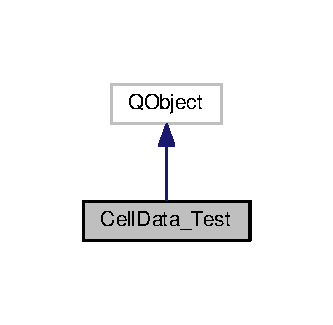
\includegraphics[width=160pt]{class_cell_data___test__inherit__graph}
\end{center}
\end{figure}


Collaboration diagram for Cell\+Data\+\_\+\+Test\+:
\nopagebreak
\begin{figure}[H]
\begin{center}
\leavevmode
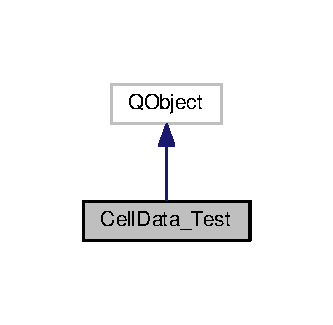
\includegraphics[width=160pt]{class_cell_data___test__coll__graph}
\end{center}
\end{figure}
\subsection*{Public Member Functions}
\begin{DoxyCompactItemize}
\item 
{\bfseries Cell\+Data\+\_\+\+Test} (\hyperlink{class_app_settings}{App\+Settings} $\ast$app\+Settings, Q\+Object $\ast$parent=0)\hypertarget{class_cell_data___test_a90979511947668d5a7f6dc56ec19b0d8}{}\label{class_cell_data___test_a90979511947668d5a7f6dc56ec19b0d8}

\item 
void {\bfseries set\+Project\+Reader\+Writer} (\hyperlink{class_project_reader_writer}{Project\+Reader\+Writer} $\ast$value)\hypertarget{class_cell_data___test_ac76aa860bdb9f80976fd59632e423c0d}{}\label{class_cell_data___test_ac76aa860bdb9f80976fd59632e423c0d}

\end{DoxyCompactItemize}
\subsection*{Public Attributes}
\begin{DoxyCompactItemize}
\item 
Q\+String {\bfseries cell\+Name1} = \char`\"{}cell11\char`\"{}\hypertarget{class_cell_data___test_a86576f8a420db7fff54f3c0bd38e1940}{}\label{class_cell_data___test_a86576f8a420db7fff54f3c0bd38e1940}

\item 
Q\+String {\bfseries cell\+Name2} = \char`\"{}cell33\char`\"{}\hypertarget{class_cell_data___test_aabefe6fe19a4cc66b60cbc154aeb9192}{}\label{class_cell_data___test_aabefe6fe19a4cc66b60cbc154aeb9192}

\item 
Q\+String {\bfseries center\+Name1} = \char`\"{}Center11\char`\"{}\hypertarget{class_cell_data___test_a34e4a8f6576f453dd74b82fcd6b5b5b0}{}\label{class_cell_data___test_a34e4a8f6576f453dd74b82fcd6b5b5b0}

\item 
Q\+String {\bfseries center\+Name2} = \char`\"{}Center33\char`\"{}\hypertarget{class_cell_data___test_aa739f167cf2f061a81914f11b00336ba}{}\label{class_cell_data___test_aa739f167cf2f061a81914f11b00336ba}

\item 
Q\+String {\bfseries test\+Operators\+File} = \char`\"{}operators\char`\"{}\hypertarget{class_cell_data___test_ad719148dc874dfe5b34774a16727a65d}{}\label{class_cell_data___test_ad719148dc874dfe5b34774a16727a65d}

\item 
int {\bfseries test\+Number1} = 11\hypertarget{class_cell_data___test_a6b7490679330fed347ee065fc1f9d501}{}\label{class_cell_data___test_a6b7490679330fed347ee065fc1f9d501}

\item 
float {\bfseries test\+Number2} = 6900\hypertarget{class_cell_data___test_a60ec71bcced5a5010bb7face873cad3a}{}\label{class_cell_data___test_a60ec71bcced5a5010bb7face873cad3a}

\item 
Q\+String {\bfseries test\+Project\+Name} = \char`\"{}test\char`\"{}\hypertarget{class_cell_data___test_a3b7dcd0ebe102cc1694f5c9c29f8eddc}{}\label{class_cell_data___test_a3b7dcd0ebe102cc1694f5c9c29f8eddc}

\item 
Q\+String {\bfseries test\+Project\+Dir} = \char`\"{}projects\char`\"{}\hypertarget{class_cell_data___test_a295f782a4b9164b7e4561159729e3480}{}\label{class_cell_data___test_a295f782a4b9164b7e4561159729e3480}

\item 
const char $\ast$ {\bfseries test\+Phrase} = \char`\"{}cell11\char`\"{}\hypertarget{class_cell_data___test_a2c7d11cc027bdc26b7fec6a809989410}{}\label{class_cell_data___test_a2c7d11cc027bdc26b7fec6a809989410}

\end{DoxyCompactItemize}


The documentation for this class was generated from the following files\+:\begin{DoxyCompactItemize}
\item 
/home/trance/\+L\+T\+Esim/\+Internal.\+L\+T\+Esim\+Generator/\+L\+T\+Esim\+Generator\+G\+U\+I/\+Maps/\+Traffic/\+Map\+Test/\+Data\+Objects\+Test/\+Cell\+Data\+Test/celldata\+\_\+test.\+h\item 
/home/trance/\+L\+T\+Esim/\+Internal.\+L\+T\+Esim\+Generator/\+L\+T\+Esim\+Generator\+G\+U\+I/\+Maps/\+Traffic/\+Map\+Test/\+Data\+Objects\+Test/\+Cell\+Data\+Test/celldata\+\_\+test.\+cpp\end{DoxyCompactItemize}

\hypertarget{structcell_name}{}\section{cell\+Name Struct Reference}
\label{structcell_name}\index{cell\+Name@{cell\+Name}}


Collaboration diagram for cell\+Name\+:
\nopagebreak
\begin{figure}[H]
\begin{center}
\leavevmode
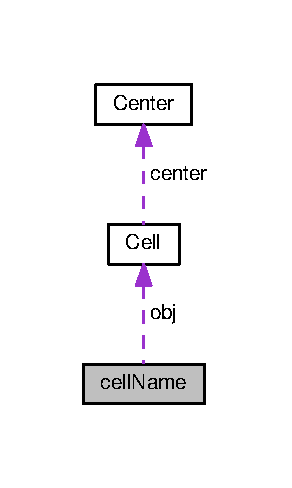
\includegraphics[width=140pt]{structcell_name__coll__graph}
\end{center}
\end{figure}
\subsection*{Public Attributes}
\begin{DoxyCompactItemize}
\item 
\hyperlink{class_cell}{Cell} $\ast$ {\bfseries obj}\hypertarget{structcell_name_a127eb40699418eb2d0c366af3c432d70}{}\label{structcell_name_a127eb40699418eb2d0c366af3c432d70}

\item 
Q\+String {\bfseries name}\hypertarget{structcell_name_aacec58e68a6e50aea041ec8848e0639f}{}\label{structcell_name_aacec58e68a6e50aea041ec8848e0639f}

\end{DoxyCompactItemize}


The documentation for this struct was generated from the following file\+:\begin{DoxyCompactItemize}
\item 
/home/trance/\+L\+T\+Esim/\+Internal.\+L\+T\+Esim\+Generator/\+L\+T\+Esim\+Generator\+G\+U\+I/\+Management\+Window/\+Encryption/encryption.\+h\end{DoxyCompactItemize}

\hypertarget{struct_cell_params}{}\section{Cell\+Params Struct Reference}
\label{struct_cell_params}\index{Cell\+Params@{Cell\+Params}}


Collaboration diagram for Cell\+Params\+:
\nopagebreak
\begin{figure}[H]
\begin{center}
\leavevmode
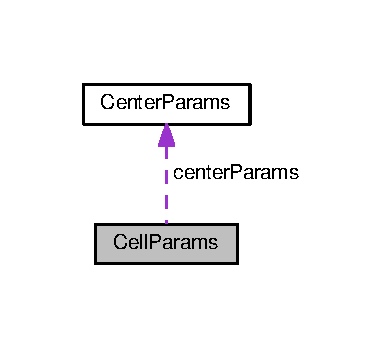
\includegraphics[width=184pt]{struct_cell_params__coll__graph}
\end{center}
\end{figure}
\subsection*{Public Attributes}
\begin{DoxyCompactItemize}
\item 
Q\+String {\bfseries cell\+Name}\hypertarget{struct_cell_params_a683f32d70a8f1e0a364fab6537c99de2}{}\label{struct_cell_params_a683f32d70a8f1e0a364fab6537c99de2}

\item 
Q\+Point {\bfseries cell\+Position}\hypertarget{struct_cell_params_a7411bd09eae01c50074afc983c36510f}{}\label{struct_cell_params_a7411bd09eae01c50074afc983c36510f}

\item 
float {\bfseries transmit\+Power}\hypertarget{struct_cell_params_adbec6f87448137812039080c464f0fee}{}\label{struct_cell_params_adbec6f87448137812039080c464f0fee}

\item 
float {\bfseries ul\+Noise\+And\+Interference}\hypertarget{struct_cell_params_a3aedfa515c2024ef0837d68f25675bd4}{}\label{struct_cell_params_a3aedfa515c2024ef0837d68f25675bd4}

\item 
int {\bfseries pci}\hypertarget{struct_cell_params_af743090f488d8a21de0c0c54b32344e0}{}\label{struct_cell_params_af743090f488d8a21de0c0c54b32344e0}

\item 
int {\bfseries earfcn\+Dl}\hypertarget{struct_cell_params_acd36b0442e14509df10b16e2e6aa811a}{}\label{struct_cell_params_acd36b0442e14509df10b16e2e6aa811a}

\item 
\hyperlink{struct_center_params}{Center\+Params} {\bfseries center\+Params}\hypertarget{struct_cell_params_a431944f5cdb2a391387a7a01157e4941}{}\label{struct_cell_params_a431944f5cdb2a391387a7a01157e4941}

\end{DoxyCompactItemize}


The documentation for this struct was generated from the following file\+:\begin{DoxyCompactItemize}
\item 
/home/trance/\+L\+T\+Esim/\+Internal.\+L\+T\+Esim\+Generator/\+L\+T\+Esim\+Generator\+G\+U\+I/\+Maps/\+Traffic/\+Data\+Objects/celldata.\+h\end{DoxyCompactItemize}

\hypertarget{class_center}{}\section{Center Class Reference}
\label{class_center}\index{Center@{Center}}
\subsection*{Public Member Functions}
\begin{DoxyCompactItemize}
\item 
{\bfseries Center} (Q\+String name)\hypertarget{class_center_aa9cce441a9ac92e67bd957af94f3836f}{}\label{class_center_aa9cce441a9ac92e67bd957af94f3836f}

\item 
Q\+String {\bfseries get\+Area} ()\hypertarget{class_center_ac2b26e1ae67cc22cd2077c8b895cf132}{}\label{class_center_ac2b26e1ae67cc22cd2077c8b895cf132}

\item 
Q\+String {\bfseries get\+South\+Boundary} ()\hypertarget{class_center_a61d8edb5d5a9b4100e6b5e3ed53ceed5}{}\label{class_center_a61d8edb5d5a9b4100e6b5e3ed53ceed5}

\item 
Q\+String {\bfseries get\+North\+Boundary} ()\hypertarget{class_center_a501b1cb19923037782e36c973b6fb582}{}\label{class_center_a501b1cb19923037782e36c973b6fb582}

\item 
Q\+String {\bfseries get\+West\+Boundary} ()\hypertarget{class_center_a3cd74f7943e6d8bf1a2724496292a985}{}\label{class_center_a3cd74f7943e6d8bf1a2724496292a985}

\item 
Q\+String {\bfseries get\+East\+Boundary} ()\hypertarget{class_center_a03da519bedb55583269a378d05e63550}{}\label{class_center_a03da519bedb55583269a378d05e63550}

\item 
void {\bfseries set\+Area} (Q\+String value)\hypertarget{class_center_a883998adf0797e31586b3f31f9951b65}{}\label{class_center_a883998adf0797e31586b3f31f9951b65}

\item 
void {\bfseries set\+South\+Boundary} (Q\+String s)\hypertarget{class_center_a23a2167660e69020b6dc6b9da834dc8a}{}\label{class_center_a23a2167660e69020b6dc6b9da834dc8a}

\item 
void {\bfseries set\+North\+Boundary} (Q\+String n)\hypertarget{class_center_aa73c1df32c9ada2775823f3e5be37674}{}\label{class_center_aa73c1df32c9ada2775823f3e5be37674}

\item 
void {\bfseries set\+West\+Boundary} (Q\+String w)\hypertarget{class_center_a51b698ef4f9dc546e424f407227d1312}{}\label{class_center_a51b698ef4f9dc546e424f407227d1312}

\item 
void {\bfseries set\+East\+Boundary} (Q\+String e)\hypertarget{class_center_a3ab8f4cb137afd4c761f40897708bf66}{}\label{class_center_a3ab8f4cb137afd4c761f40897708bf66}

\item 
bool {\bfseries was\+There\+Parameters\+Change} ()\hypertarget{class_center_a20e04053568aba3080700405fa300836}{}\label{class_center_a20e04053568aba3080700405fa300836}

\item 
void {\bfseries reset\+Params} ()\hypertarget{class_center_ae2022a3991d768457d0fea5ed770806b}{}\label{class_center_ae2022a3991d768457d0fea5ed770806b}

\item 
Q\+String {\bfseries get\+New\+\_\+name\+\_\+area} () const \hypertarget{class_center_a32d7edd54da76cd8df24ddedb19a5e6b}{}\label{class_center_a32d7edd54da76cd8df24ddedb19a5e6b}

\item 
void {\bfseries set\+New\+\_\+name\+\_\+area} (const Q\+String \&value)\hypertarget{class_center_a6187917c791160f679e266c81f1dd41b}{}\label{class_center_a6187917c791160f679e266c81f1dd41b}

\end{DoxyCompactItemize}


The documentation for this class was generated from the following files\+:\begin{DoxyCompactItemize}
\item 
/home/trance/\+L\+T\+Esim/\+Internal.\+L\+T\+Esim\+Generator/\+L\+T\+Esim\+Generator\+G\+U\+I/\+Maps/\+Map\+Objects/center.\+h\item 
/home/trance/\+L\+T\+Esim/\+Internal.\+L\+T\+Esim\+Generator/\+L\+T\+Esim\+Generator\+G\+U\+I/\+Maps/\+Map\+Objects/center.\+cpp\end{DoxyCompactItemize}

\hypertarget{structcenter_name}{}\section{center\+Name Struct Reference}
\label{structcenter_name}\index{center\+Name@{center\+Name}}


Collaboration diagram for center\+Name\+:
\nopagebreak
\begin{figure}[H]
\begin{center}
\leavevmode
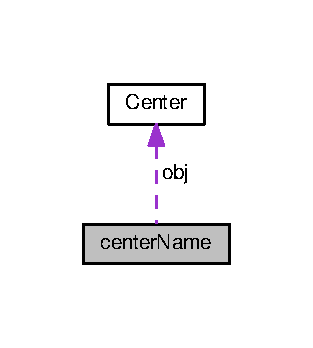
\includegraphics[width=150pt]{structcenter_name__coll__graph}
\end{center}
\end{figure}
\subsection*{Public Attributes}
\begin{DoxyCompactItemize}
\item 
\hyperlink{class_center}{Center} $\ast$ {\bfseries obj}\hypertarget{structcenter_name_a8224393b959591c56b9d46b29ad43098}{}\label{structcenter_name_a8224393b959591c56b9d46b29ad43098}

\item 
Q\+String {\bfseries name}\hypertarget{structcenter_name_aba5ff6b06f58f2b0fce0ee81bf0cb624}{}\label{structcenter_name_aba5ff6b06f58f2b0fce0ee81bf0cb624}

\end{DoxyCompactItemize}


The documentation for this struct was generated from the following file\+:\begin{DoxyCompactItemize}
\item 
/home/trance/\+L\+T\+Esim/\+Internal.\+L\+T\+Esim\+Generator/\+L\+T\+Esim\+Generator\+G\+U\+I/\+Management\+Window/\+Encryption/encryption.\+h\end{DoxyCompactItemize}

\hypertarget{struct_center_params}{}\section{Center\+Params Struct Reference}
\label{struct_center_params}\index{Center\+Params@{Center\+Params}}
\subsection*{Public Attributes}
\begin{DoxyCompactItemize}
\item 
Q\+String {\bfseries center\+Name}\hypertarget{struct_center_params_a8050ad435eb184a5caf881cc041dafb6}{}\label{struct_center_params_a8050ad435eb184a5caf881cc041dafb6}

\item 
Q\+Rect {\bfseries center\+Area}\hypertarget{struct_center_params_a1dbf7f75db4b194eb0be2f3699bcd477}{}\label{struct_center_params_a1dbf7f75db4b194eb0be2f3699bcd477}

\end{DoxyCompactItemize}


The documentation for this struct was generated from the following file\+:\begin{DoxyCompactItemize}
\item 
/home/trance/\+L\+T\+Esim/\+Internal.\+L\+T\+Esim\+Generator/\+L\+T\+Esim\+Generator\+G\+U\+I/\+Maps/\+Traffic/\+Data\+Objects/celldata.\+h\end{DoxyCompactItemize}

\hypertarget{struct_change}{}\section{Change Struct Reference}
\label{struct_change}\index{Change@{Change}}
\subsection*{Public Attributes}
\begin{DoxyCompactItemize}
\item 
Q\+String {\bfseries type}\hypertarget{struct_change_a540497453596308a68e15532ca23ffd1}{}\label{struct_change_a540497453596308a68e15532ca23ffd1}

\item 
int {\bfseries pos}\hypertarget{struct_change_a8328d66176b9af8693380b9d790ed055}{}\label{struct_change_a8328d66176b9af8693380b9d790ed055}

\item 
int {\bfseries length}\hypertarget{struct_change_ab60176801fef8803c8e4e93b3096e4c8}{}\label{struct_change_ab60176801fef8803c8e4e93b3096e4c8}

\item 
Q\+String {\bfseries content}\hypertarget{struct_change_ac738ff8bc630d9955a213177065618d4}{}\label{struct_change_ac738ff8bc630d9955a213177065618d4}

\end{DoxyCompactItemize}


The documentation for this struct was generated from the following file\+:\begin{DoxyCompactItemize}
\item 
/home/trance/\+L\+T\+Esim/\+Internal.\+L\+T\+Esim\+Generator/\+L\+T\+Esim\+Generator\+G\+U\+I/\+Management\+Window/\+Parameters\+Window/parameterswindow.\+cpp\end{DoxyCompactItemize}

\hypertarget{class_channel_model}{}\section{Channel\+Model Class Reference}
\label{class_channel_model}\index{Channel\+Model@{Channel\+Model}}
\subsection*{Public Member Functions}
\begin{DoxyCompactItemize}
\item 
Q\+String {\bfseries get\+Model\+\_\+set\+\_\+name} ()\hypertarget{class_channel_model_a47e90cc85542a4832b5b01a535dfd769}{}\label{class_channel_model_a47e90cc85542a4832b5b01a535dfd769}

\item 
void {\bfseries set\+Model\+\_\+set\+\_\+name} (Q\+String value)\hypertarget{class_channel_model_ad9460d253362deaa0bdae23611ab25cb}{}\label{class_channel_model_ad9460d253362deaa0bdae23611ab25cb}

\item 
Q\+String {\bfseries get\+Pdcch\+\_\+drop\+\_\+dl\+\_\+assignment\+\_\+rate} () const \hypertarget{class_channel_model_a66251d1d429b44ffcdfe88b5b0394f20}{}\label{class_channel_model_a66251d1d429b44ffcdfe88b5b0394f20}

\item 
void {\bfseries set\+Pdcch\+\_\+drop\+\_\+dl\+\_\+assignment\+\_\+rate} (Q\+String value)\hypertarget{class_channel_model_a65b9df4da57a3bf781d883c7a69e8e47}{}\label{class_channel_model_a65b9df4da57a3bf781d883c7a69e8e47}

\item 
Q\+String {\bfseries get\+Pdcch\+\_\+drop\+\_\+grant\+\_\+rate} () const \hypertarget{class_channel_model_ae61c0591404f59884a596dacf4ddcff1}{}\label{class_channel_model_ae61c0591404f59884a596dacf4ddcff1}

\item 
void {\bfseries set\+Pdcch\+\_\+drop\+\_\+grant\+\_\+rate} (Q\+String value)\hypertarget{class_channel_model_a776b919d80e8ac1ffa7d69eff6b27d2f}{}\label{class_channel_model_a776b919d80e8ac1ffa7d69eff6b27d2f}

\item 
Q\+String {\bfseries get\+Pdsch\+\_\+transport\+\_\+block\+\_\+decoded\+\_\+error\+\_\+rate} () const \hypertarget{class_channel_model_a7ed0521786b53a53e5e35700e4d086a3}{}\label{class_channel_model_a7ed0521786b53a53e5e35700e4d086a3}

\item 
void {\bfseries set\+Pdsch\+\_\+transport\+\_\+block\+\_\+decoded\+\_\+error\+\_\+rate} (Q\+String value)\hypertarget{class_channel_model_af2aa3eefdcd0b12b8a05e5e744739beb}{}\label{class_channel_model_af2aa3eefdcd0b12b8a05e5e744739beb}

\item 
Q\+String {\bfseries get\+Phich\+\_\+nack\+\_\+to\+\_\+ack\+\_\+error\+\_\+rate} () const \hypertarget{class_channel_model_a7f74c61a595816fbaa6e984463481468}{}\label{class_channel_model_a7f74c61a595816fbaa6e984463481468}

\item 
void {\bfseries set\+Phich\+\_\+nack\+\_\+to\+\_\+ack\+\_\+error\+\_\+rate} (Q\+String value)\hypertarget{class_channel_model_a8674c3b5df893e1ac1ce0bad20396f72}{}\label{class_channel_model_a8674c3b5df893e1ac1ce0bad20396f72}

\item 
Q\+String {\bfseries get\+Phich\+\_\+drop\+\_\+harq\+\_\+feedback\+\_\+rate} () const \hypertarget{class_channel_model_a776261ddef7703f0051894a1b42a43a9}{}\label{class_channel_model_a776261ddef7703f0051894a1b42a43a9}

\item 
void {\bfseries set\+Phich\+\_\+drop\+\_\+harq\+\_\+feedback\+\_\+rate} (Q\+String value)\hypertarget{class_channel_model_a9299679e312459d5f1e3cd32ec1af32d}{}\label{class_channel_model_a9299679e312459d5f1e3cd32ec1af32d}

\item 
Q\+String {\bfseries get\+Pusch\+\_\+transport\+\_\+block\+\_\+decoded\+\_\+error\+\_\+rate} () const \hypertarget{class_channel_model_a41f01b0e638ad55105670c36db050f39}{}\label{class_channel_model_a41f01b0e638ad55105670c36db050f39}

\item 
void {\bfseries set\+Pusch\+\_\+transport\+\_\+block\+\_\+decoded\+\_\+error\+\_\+rate} (Q\+String value)\hypertarget{class_channel_model_a1bc2f260af96252f04af7e2a34dde132}{}\label{class_channel_model_a1bc2f260af96252f04af7e2a34dde132}

\item 
Q\+String {\bfseries get\+Pusch\+\_\+drop\+\_\+transport\+\_\+block\+\_\+rate} () const \hypertarget{class_channel_model_afce214409f20400730aae94efbd8d604}{}\label{class_channel_model_afce214409f20400730aae94efbd8d604}

\item 
void {\bfseries set\+Pusch\+\_\+drop\+\_\+transport\+\_\+block\+\_\+rate} (Q\+String value)\hypertarget{class_channel_model_a8bd50476025b1aeb01bab5e919ce6fe5}{}\label{class_channel_model_a8bd50476025b1aeb01bab5e919ce6fe5}

\item 
Q\+String {\bfseries get\+Puxch\+\_\+nack\+\_\+to\+\_\+ack\+\_\+error\+\_\+rate} () const \hypertarget{class_channel_model_a9c4ced96f975c67b3c8a27840572964e}{}\label{class_channel_model_a9c4ced96f975c67b3c8a27840572964e}

\item 
void {\bfseries set\+Puxch\+\_\+nack\+\_\+to\+\_\+ack\+\_\+error\+\_\+rate} (Q\+String value)\hypertarget{class_channel_model_aec43edbca27f694cfd5f525da1281e1d}{}\label{class_channel_model_aec43edbca27f694cfd5f525da1281e1d}

\item 
Q\+String {\bfseries get\+Puxch\+\_\+dtx\+\_\+to\+\_\+ack\+\_\+error\+\_\+rate} () const \hypertarget{class_channel_model_af785f54eaa70665cab8613d7fecfc89d}{}\label{class_channel_model_af785f54eaa70665cab8613d7fecfc89d}

\item 
void {\bfseries set\+Puxch\+\_\+dtx\+\_\+to\+\_\+ack\+\_\+error\+\_\+rate} (Q\+String value)\hypertarget{class_channel_model_a4eb360104700d0849275ab97fa76384c}{}\label{class_channel_model_a4eb360104700d0849275ab97fa76384c}

\item 
Q\+String {\bfseries get\+Puxch\+\_\+ack\+\_\+to\+\_\+nack\+\_\+error\+\_\+rate} () const \hypertarget{class_channel_model_a1d5a76c3a6ec6ef1ada1ba6efd6b8081}{}\label{class_channel_model_a1d5a76c3a6ec6ef1ada1ba6efd6b8081}

\item 
void {\bfseries set\+Puxch\+\_\+ack\+\_\+to\+\_\+nack\+\_\+error\+\_\+rate} (Q\+String value)\hypertarget{class_channel_model_ae9db999dd8ea44d564a71ef891dacc74}{}\label{class_channel_model_ae9db999dd8ea44d564a71ef891dacc74}

\item 
Q\+String {\bfseries get\+Puxch\+\_\+drop\+\_\+scheduling\+\_\+request\+\_\+rate} () const \hypertarget{class_channel_model_a0963c6ee35179ce083add9483b611349}{}\label{class_channel_model_a0963c6ee35179ce083add9483b611349}

\item 
void {\bfseries set\+Puxch\+\_\+drop\+\_\+scheduling\+\_\+request\+\_\+rate} (Q\+String value)\hypertarget{class_channel_model_afeb784c70aa3fafd4c68377493ce1363}{}\label{class_channel_model_afeb784c70aa3fafd4c68377493ce1363}

\item 
Q\+String {\bfseries get\+Dlni\+\_\+noise} () const \hypertarget{class_channel_model_a67d6b3f5aa202208b36e88354343603f}{}\label{class_channel_model_a67d6b3f5aa202208b36e88354343603f}

\item 
void {\bfseries set\+Dlni\+\_\+noise} (Q\+String value)\hypertarget{class_channel_model_afbb90279c112f50d2106844c5fe4e1f2}{}\label{class_channel_model_afbb90279c112f50d2106844c5fe4e1f2}

\item 
Q\+String {\bfseries get\+Dlni\+\_\+interference} () const \hypertarget{class_channel_model_a24411bc470d92480ad7f15d602b8d774}{}\label{class_channel_model_a24411bc470d92480ad7f15d602b8d774}

\item 
void {\bfseries set\+Dlni\+\_\+interference} (Q\+String value)\hypertarget{class_channel_model_ab936e94283d3cea954af75cafed9675e}{}\label{class_channel_model_ab936e94283d3cea954af75cafed9675e}

\item 
Q\+String {\bfseries get\+Dl\+\_\+pathloss\+\_\+min\+\_\+pathloss} () const \hypertarget{class_channel_model_abff8a3ce81e716e213947eff3cdb6591}{}\label{class_channel_model_abff8a3ce81e716e213947eff3cdb6591}

\item 
void {\bfseries set\+Dl\+\_\+pathloss\+\_\+min\+\_\+pathloss} (Q\+String value)\hypertarget{class_channel_model_a6a41fa959fc8b756203ca95963b7e62a}{}\label{class_channel_model_a6a41fa959fc8b756203ca95963b7e62a}

\item 
Q\+String {\bfseries get\+Dl\+\_\+pathloss\+\_\+max\+\_\+pathloss} () const \hypertarget{class_channel_model_a90b5fc0b2a7859044ffa9bf4c514d846}{}\label{class_channel_model_a90b5fc0b2a7859044ffa9bf4c514d846}

\item 
void {\bfseries set\+Dl\+\_\+pathloss\+\_\+max\+\_\+pathloss} (Q\+String value)\hypertarget{class_channel_model_afdcd481539e0b560731cbe0c1c1bca77}{}\label{class_channel_model_afdcd481539e0b560731cbe0c1c1bca77}

\item 
Q\+String {\bfseries get\+Dl\+\_\+pathloss\+\_\+time\+\_\+min\+\_\+to\+\_\+max} () const \hypertarget{class_channel_model_ab62eb20bf53dca5089209f86b62ec297}{}\label{class_channel_model_ab62eb20bf53dca5089209f86b62ec297}

\item 
void {\bfseries set\+Dl\+\_\+pathloss\+\_\+time\+\_\+min\+\_\+to\+\_\+max} (Q\+String value)\hypertarget{class_channel_model_a9754be20530ae597841bd2e089105d5e}{}\label{class_channel_model_a9754be20530ae597841bd2e089105d5e}

\item 
bool {\bfseries get\+Dl\+\_\+pathloss\+\_\+distribute\+\_\+ues} () const \hypertarget{class_channel_model_ab5abe9f64753c2337c50ed2e41df2590}{}\label{class_channel_model_ab5abe9f64753c2337c50ed2e41df2590}

\item 
void {\bfseries set\+Dl\+\_\+pathloss\+\_\+distribute\+\_\+ues} (bool value)\hypertarget{class_channel_model_a02523ac96840775d480f2ef7a81922c3}{}\label{class_channel_model_a02523ac96840775d480f2ef7a81922c3}

\item 
Q\+String {\bfseries get\+Pathloss\+\_\+based\+\_\+feedback\+\_\+sinr\+\_\+threshold} () const \hypertarget{class_channel_model_a88f6550fe468fdedca79d495b433b863}{}\label{class_channel_model_a88f6550fe468fdedca79d495b433b863}

\item 
void {\bfseries set\+Pathloss\+\_\+based\+\_\+feedback\+\_\+sinr\+\_\+threshold} (Q\+String value)\hypertarget{class_channel_model_ac779db5ceaa77d25326950c509f2e4c7}{}\label{class_channel_model_ac779db5ceaa77d25326950c509f2e4c7}

\item 
void {\bfseries reset\+Params} ()\hypertarget{class_channel_model_a483456aa92195b123cb747b31c525db9}{}\label{class_channel_model_a483456aa92195b123cb747b31c525db9}

\end{DoxyCompactItemize}


The documentation for this class was generated from the following files\+:\begin{DoxyCompactItemize}
\item 
/home/trance/\+L\+T\+Esim/\+Internal.\+L\+T\+Esim\+Generator/\+L\+T\+Esim\+Generator\+G\+U\+I/\+Maps/\+Parameters/\+Channel\+Model/channelmodel.\+h\item 
/home/trance/\+L\+T\+Esim/\+Internal.\+L\+T\+Esim\+Generator/\+L\+T\+Esim\+Generator\+G\+U\+I/\+Maps/\+Parameters/\+Channel\+Model/channelmodel.\+cpp\end{DoxyCompactItemize}

\hypertarget{class_channel_model_form}{}\section{Channel\+Model\+Form Class Reference}
\label{class_channel_model_form}\index{Channel\+Model\+Form@{Channel\+Model\+Form}}


Inheritance diagram for Channel\+Model\+Form\+:
\nopagebreak
\begin{figure}[H]
\begin{center}
\leavevmode
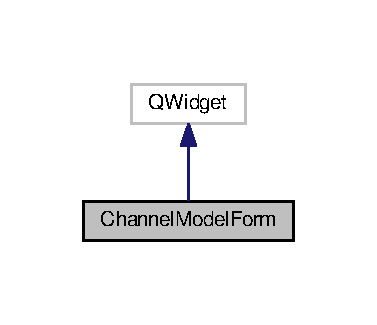
\includegraphics[width=181pt]{class_channel_model_form__inherit__graph}
\end{center}
\end{figure}


Collaboration diagram for Channel\+Model\+Form\+:
\nopagebreak
\begin{figure}[H]
\begin{center}
\leavevmode
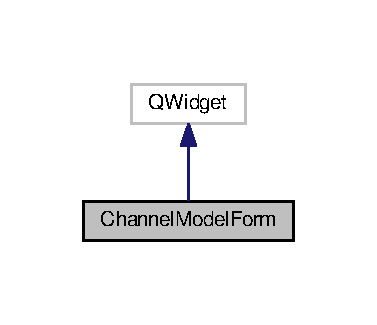
\includegraphics[width=181pt]{class_channel_model_form__coll__graph}
\end{center}
\end{figure}
\subsection*{Public Member Functions}
\begin{DoxyCompactItemize}
\item 
{\bfseries Channel\+Model\+Form} (Q\+Widget $\ast$parent=0)\hypertarget{class_channel_model_form_aa46c9d658def4f8771c16c4c8cf46053}{}\label{class_channel_model_form_aa46c9d658def4f8771c16c4c8cf46053}

\item 
void {\bfseries set\+Parameters} (\hyperlink{class_channel_model}{Channel\+Model} $\ast$chmod)\hypertarget{class_channel_model_form_acd2695fd71d1148450792cc0fa9f0b35}{}\label{class_channel_model_form_acd2695fd71d1148450792cc0fa9f0b35}

\end{DoxyCompactItemize}


The documentation for this class was generated from the following files\+:\begin{DoxyCompactItemize}
\item 
/home/trance/\+L\+T\+Esim/\+Internal.\+L\+T\+Esim\+Generator/\+L\+T\+Esim\+Generator\+G\+U\+I/\+Maps/\+Parameters/\+Channel\+Model/channelmodelform.\+h\item 
/home/trance/\+L\+T\+Esim/\+Internal.\+L\+T\+Esim\+Generator/\+L\+T\+Esim\+Generator\+G\+U\+I/\+Maps/\+Parameters/\+Channel\+Model/channelmodelform.\+cpp\end{DoxyCompactItemize}

\hypertarget{class_composition_of_areas}{}\section{Composition\+Of\+Areas Class Reference}
\label{class_composition_of_areas}\index{Composition\+Of\+Areas@{Composition\+Of\+Areas}}


Inheritance diagram for Composition\+Of\+Areas\+:
\nopagebreak
\begin{figure}[H]
\begin{center}
\leavevmode
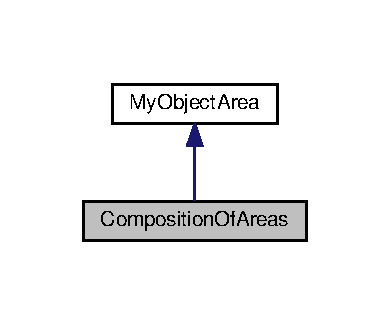
\includegraphics[width=187pt]{class_composition_of_areas__inherit__graph}
\end{center}
\end{figure}


Collaboration diagram for Composition\+Of\+Areas\+:
\nopagebreak
\begin{figure}[H]
\begin{center}
\leavevmode
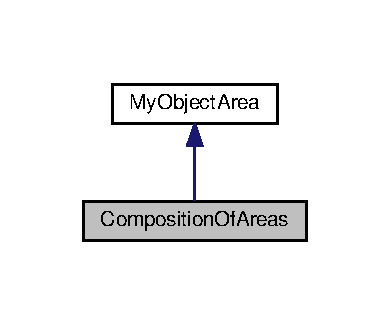
\includegraphics[width=187pt]{class_composition_of_areas__coll__graph}
\end{center}
\end{figure}
\subsection*{Public Member Functions}
\begin{DoxyCompactItemize}
\item 
bool {\bfseries contain} (int x\+Pos, int y\+Pos, \hyperlink{class_my_object_area}{My\+Object\+Area} $\ast$$\ast$obj\+Ptr1)\hypertarget{class_composition_of_areas_aad6ff29c838a7b9aceaa48638c9249da}{}\label{class_composition_of_areas_aad6ff29c838a7b9aceaa48638c9249da}

\item 
Q\+String {\bfseries get\+ID} ()\hypertarget{class_composition_of_areas_aef1b4af535f22f35c5d6bfb91230754e}{}\label{class_composition_of_areas_aef1b4af535f22f35c5d6bfb91230754e}

\item 
void {\bfseries add\+To\+List} (\hyperlink{class_my_object_area}{My\+Object\+Area} $\ast$object)\hypertarget{class_composition_of_areas_a466347d7848229c6bec2f6b8f492bde0}{}\label{class_composition_of_areas_a466347d7848229c6bec2f6b8f492bde0}

\item 
int {\bfseries size} ()\hypertarget{class_composition_of_areas_a2afe45db6f26b3fcd68bc27bc199b811}{}\label{class_composition_of_areas_a2afe45db6f26b3fcd68bc27bc199b811}

\end{DoxyCompactItemize}
\subsection*{Public Attributes}
\begin{DoxyCompactItemize}
\item 
Q\+Vector$<$ \hyperlink{class_my_object_area}{My\+Object\+Area} $\ast$ $>$ {\bfseries area\+List}\hypertarget{class_composition_of_areas_aaceb49cf077b77910375af9a3b52f777}{}\label{class_composition_of_areas_aaceb49cf077b77910375af9a3b52f777}

\end{DoxyCompactItemize}


The documentation for this class was generated from the following file\+:\begin{DoxyCompactItemize}
\item 
/home/trance/\+L\+T\+Esim/\+Internal.\+L\+T\+Esim\+Generator/\+L\+T\+Esim\+Generator\+G\+U\+I/\+Maps/\+Traffic/\+Map\+Components/compositionofareas.\+h\end{DoxyCompactItemize}

\hypertarget{class_composition_of_areas___test}{}\section{Composition\+Of\+Areas\+\_\+\+Test Class Reference}
\label{class_composition_of_areas___test}\index{Composition\+Of\+Areas\+\_\+\+Test@{Composition\+Of\+Areas\+\_\+\+Test}}


Inheritance diagram for Composition\+Of\+Areas\+\_\+\+Test\+:
\nopagebreak
\begin{figure}[H]
\begin{center}
\leavevmode
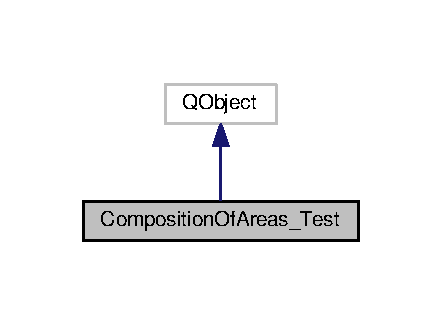
\includegraphics[width=212pt]{class_composition_of_areas___test__inherit__graph}
\end{center}
\end{figure}


Collaboration diagram for Composition\+Of\+Areas\+\_\+\+Test\+:
\nopagebreak
\begin{figure}[H]
\begin{center}
\leavevmode
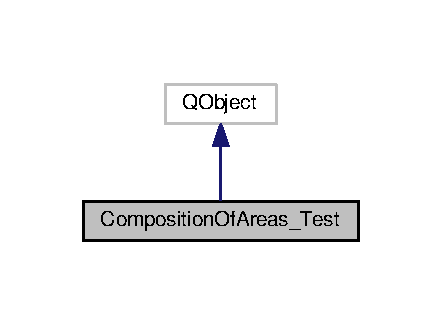
\includegraphics[width=212pt]{class_composition_of_areas___test__coll__graph}
\end{center}
\end{figure}


The documentation for this class was generated from the following files\+:\begin{DoxyCompactItemize}
\item 
/home/trance/\+L\+T\+Esim/\+Internal.\+L\+T\+Esim\+Generator/\+L\+T\+Esim\+Generator\+G\+U\+I/\+Maps/\+Traffic/\+Map\+Test/\+Map\+Components\+Test/compositionofareas\+\_\+test.\+h\item 
/home/trance/\+L\+T\+Esim/\+Internal.\+L\+T\+Esim\+Generator/\+L\+T\+Esim\+Generator\+G\+U\+I/\+Maps/\+Traffic/\+Map\+Test/\+Map\+Components\+Test/compositionofareas\+\_\+test.\+cpp\end{DoxyCompactItemize}

\hypertarget{struct_tuningtraffic_1_1_c_s_parameters}{}\section{Tuningtraffic\+:\+:C\+S\+Parameters Struct Reference}
\label{struct_tuningtraffic_1_1_c_s_parameters}\index{Tuningtraffic\+::\+C\+S\+Parameters@{Tuningtraffic\+::\+C\+S\+Parameters}}
\subsection*{Public Attributes}
\begin{DoxyCompactItemize}
\item 
Q\+String {\bfseries cs\+\_\+name}\hypertarget{struct_tuningtraffic_1_1_c_s_parameters_a2ddf44c8f2997c270cf26e3648de2bce}{}\label{struct_tuningtraffic_1_1_c_s_parameters_a2ddf44c8f2997c270cf26e3648de2bce}

\item 
Q\+String {\bfseries call\+\_\+intensity}\hypertarget{struct_tuningtraffic_1_1_c_s_parameters_adb9bce9f12ee7c1e3e2ece6160516a56}{}\label{struct_tuningtraffic_1_1_c_s_parameters_adb9bce9f12ee7c1e3e2ece6160516a56}

\item 
Q\+String {\bfseries call\+\_\+duration}\hypertarget{struct_tuningtraffic_1_1_c_s_parameters_a4cc74ce2f1b792e0ab1565e6403fa7d8}{}\label{struct_tuningtraffic_1_1_c_s_parameters_a4cc74ce2f1b792e0ab1565e6403fa7d8}

\item 
Q\+String {\bfseries recovery\+\_\+start\+\_\+interval}\hypertarget{struct_tuningtraffic_1_1_c_s_parameters_ab4629cdde3c1f7c52a5df484aa5c2c9e}{}\label{struct_tuningtraffic_1_1_c_s_parameters_ab4629cdde3c1f7c52a5df484aa5c2c9e}

\end{DoxyCompactItemize}


The documentation for this struct was generated from the following file\+:\begin{DoxyCompactItemize}
\item 
/home/trance/\+L\+T\+Esim/\+Internal.\+L\+T\+Esim\+Generator/\+L\+T\+Esim\+Generator\+G\+U\+I/\+Maps/\+Traffic/\+Tuning/tuningtraffic.\+h\end{DoxyCompactItemize}

\hypertarget{class_custom_model_label}{}\section{Custom\+Model\+Label Class Reference}
\label{class_custom_model_label}\index{Custom\+Model\+Label@{Custom\+Model\+Label}}


Inheritance diagram for Custom\+Model\+Label\+:
\nopagebreak
\begin{figure}[H]
\begin{center}
\leavevmode
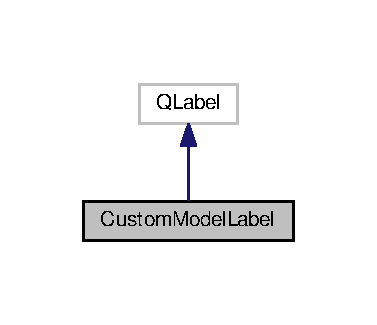
\includegraphics[width=181pt]{class_custom_model_label__inherit__graph}
\end{center}
\end{figure}


Collaboration diagram for Custom\+Model\+Label\+:
\nopagebreak
\begin{figure}[H]
\begin{center}
\leavevmode
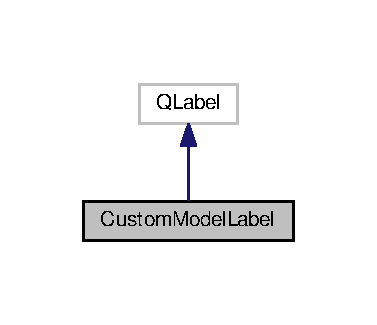
\includegraphics[width=181pt]{class_custom_model_label__coll__graph}
\end{center}
\end{figure}
\subsection*{Public Member Functions}
\begin{DoxyCompactItemize}
\item 
{\bfseries Custom\+Model\+Label} (const Q\+String \&text, Q\+Widget $\ast$parent=0)\hypertarget{class_custom_model_label_a4c14caab17949fb520c81f5940bec2d2}{}\label{class_custom_model_label_a4c14caab17949fb520c81f5940bec2d2}

\item 
void {\bfseries mouse\+Double\+Click\+Event} (Q\+Mouse\+Event $\ast$event)\hypertarget{class_custom_model_label_ac5465f245d0441c93c18d28d46409023}{}\label{class_custom_model_label_ac5465f245d0441c93c18d28d46409023}

\item 
void {\bfseries set\+Geometry} (int x, int y)\hypertarget{class_custom_model_label_a0dd26f37684ad520b4f848748c29d1c0}{}\label{class_custom_model_label_a0dd26f37684ad520b4f848748c29d1c0}

\end{DoxyCompactItemize}
\subsection*{Friends}
\begin{DoxyCompactItemize}
\item 
class {\bfseries Custom\+Model\+Label\+\_\+\+Test}\hypertarget{class_custom_model_label_a43ccaa3a8c63e19ea328e17f499ec200}{}\label{class_custom_model_label_a43ccaa3a8c63e19ea328e17f499ec200}

\end{DoxyCompactItemize}


The documentation for this class was generated from the following files\+:\begin{DoxyCompactItemize}
\item 
/home/trance/\+L\+T\+Esim/\+Internal.\+L\+T\+Esim\+Generator/\+L\+T\+Esim\+Generator\+G\+U\+I/\+Maps/\+Traffic/\+Map\+Components/custommodellabel.\+h\item 
/home/trance/\+L\+T\+Esim/\+Internal.\+L\+T\+Esim\+Generator/\+L\+T\+Esim\+Generator\+G\+U\+I/\+Maps/\+Traffic/\+Map\+Components/custommodellabel.\+cpp\end{DoxyCompactItemize}

\hypertarget{class_custom_model_label___test}{}\section{Custom\+Model\+Label\+\_\+\+Test Class Reference}
\label{class_custom_model_label___test}\index{Custom\+Model\+Label\+\_\+\+Test@{Custom\+Model\+Label\+\_\+\+Test}}


Inheritance diagram for Custom\+Model\+Label\+\_\+\+Test\+:
\nopagebreak
\begin{figure}[H]
\begin{center}
\leavevmode
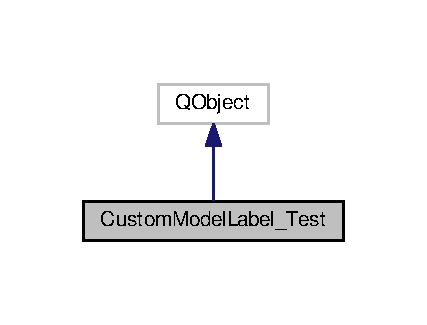
\includegraphics[width=205pt]{class_custom_model_label___test__inherit__graph}
\end{center}
\end{figure}


Collaboration diagram for Custom\+Model\+Label\+\_\+\+Test\+:
\nopagebreak
\begin{figure}[H]
\begin{center}
\leavevmode
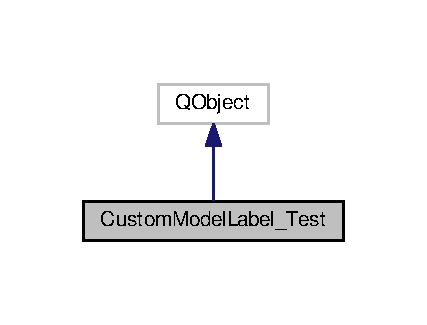
\includegraphics[width=205pt]{class_custom_model_label___test__coll__graph}
\end{center}
\end{figure}


The documentation for this class was generated from the following files\+:\begin{DoxyCompactItemize}
\item 
/home/trance/\+L\+T\+Esim/\+Internal.\+L\+T\+Esim\+Generator/\+L\+T\+Esim\+Generator\+G\+U\+I/\+Maps/\+Traffic/\+Map\+Test/\+Map\+Components\+Test/custommodellabel\+\_\+test.\+h\item 
/home/trance/\+L\+T\+Esim/\+Internal.\+L\+T\+Esim\+Generator/\+L\+T\+Esim\+Generator\+G\+U\+I/\+Maps/\+Traffic/\+Map\+Test/\+Map\+Components\+Test/custommodellabel\+\_\+test.\+cpp\end{DoxyCompactItemize}

\hypertarget{class_custommodels}{}\section{Custommodels Class Reference}
\label{class_custommodels}\index{Custommodels@{Custommodels}}


Inheritance diagram for Custommodels\+:
\nopagebreak
\begin{figure}[H]
\begin{center}
\leavevmode
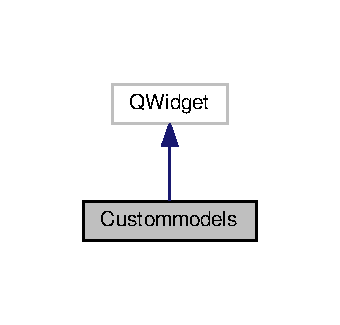
\includegraphics[width=163pt]{class_custommodels__inherit__graph}
\end{center}
\end{figure}


Collaboration diagram for Custommodels\+:
\nopagebreak
\begin{figure}[H]
\begin{center}
\leavevmode
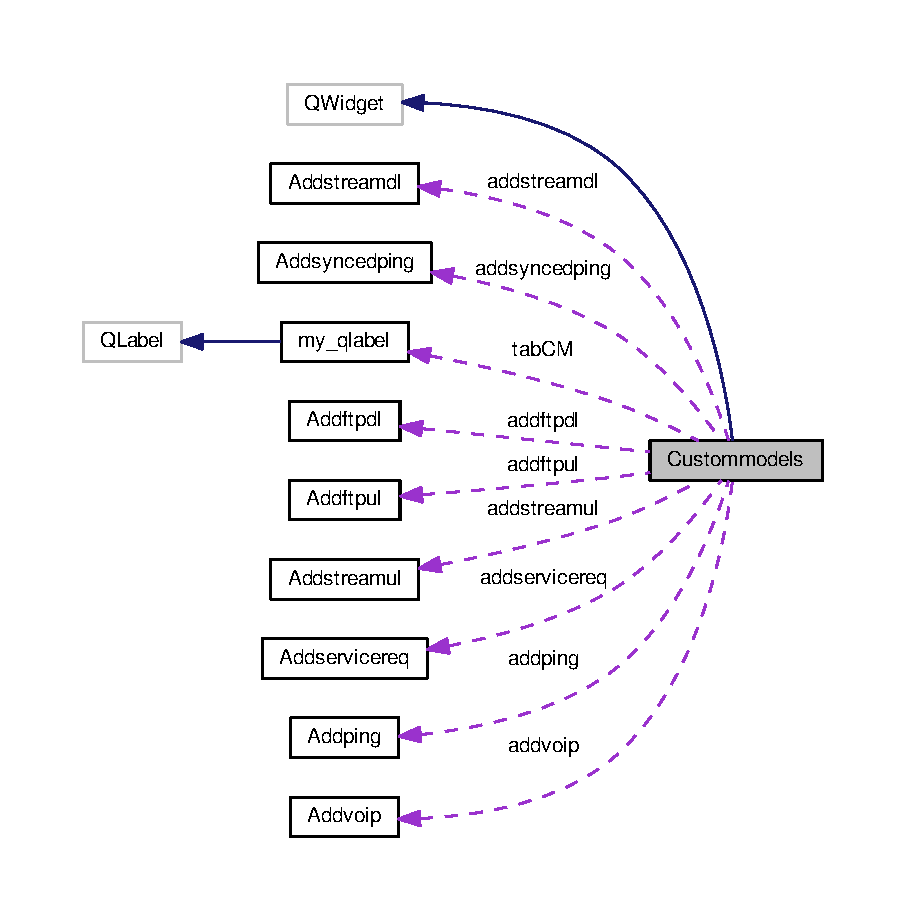
\includegraphics[width=350pt]{class_custommodels__coll__graph}
\end{center}
\end{figure}
\subsection*{Public Member Functions}
\begin{DoxyCompactItemize}
\item 
{\bfseries Custommodels} (Q\+Widget $\ast$parent=0)\hypertarget{class_custommodels_afbdddfe12335dc1a99a0df50b6d59c5e}{}\label{class_custommodels_afbdddfe12335dc1a99a0df50b6d59c5e}

\item 
void {\bfseries add\+To\+List} ()\hypertarget{class_custommodels_a0155dbcc4ecb61c4fa1ae51f78d4c7fa}{}\label{class_custommodels_a0155dbcc4ecb61c4fa1ae51f78d4c7fa}

\item 
bool {\bfseries to\+Bool} (Q\+String value)\hypertarget{class_custommodels_a9b1297a0253a388c370618b44b830858}{}\label{class_custommodels_a9b1297a0253a388c370618b44b830858}

\item 
void {\bfseries set\+\_\+custom\+\_\+name} (Q\+String name)\hypertarget{class_custommodels_a0441728f4923986aec40d09d9b927e6b}{}\label{class_custommodels_a0441728f4923986aec40d09d9b927e6b}

\item 
void {\bfseries set\+Parameters} ()\hypertarget{class_custommodels_a59e677dd38af334094efff88d9ce98ed}{}\label{class_custommodels_a59e677dd38af334094efff88d9ce98ed}

\item 
void {\bfseries start\+Parameter} ()\hypertarget{class_custommodels_af2dc416716136532ce56a1fb687a7e84}{}\label{class_custommodels_af2dc416716136532ce56a1fb687a7e84}

\end{DoxyCompactItemize}
\subsection*{Public Attributes}
\begin{DoxyCompactItemize}
\item 
\hyperlink{class_addping}{Addping} $\ast$ {\bfseries addping}\hypertarget{class_custommodels_a6ddf7b7f0de216130ac54024bd29bb9d}{}\label{class_custommodels_a6ddf7b7f0de216130ac54024bd29bb9d}

\item 
\hyperlink{class_addvoip}{Addvoip} $\ast$ {\bfseries addvoip}\hypertarget{class_custommodels_a74d65740fafd53f56ac59caa69416b08}{}\label{class_custommodels_a74d65740fafd53f56ac59caa69416b08}

\item 
\hyperlink{class_addftpdl}{Addftpdl} $\ast$ {\bfseries addftpdl}\hypertarget{class_custommodels_aa9bbefb10ee69b1404fd41464bb54e90}{}\label{class_custommodels_aa9bbefb10ee69b1404fd41464bb54e90}

\item 
\hyperlink{class_addftpul}{Addftpul} $\ast$ {\bfseries addftpul}\hypertarget{class_custommodels_a5ef9281f535e495f2d639a98bf298113}{}\label{class_custommodels_a5ef9281f535e495f2d639a98bf298113}

\item 
\hyperlink{class_addstreamdl}{Addstreamdl} $\ast$ {\bfseries addstreamdl}\hypertarget{class_custommodels_a8af449740c11d8e65b74584d150ffbed}{}\label{class_custommodels_a8af449740c11d8e65b74584d150ffbed}

\item 
\hyperlink{class_addstreamul}{Addstreamul} $\ast$ {\bfseries addstreamul}\hypertarget{class_custommodels_ab2c1698bd143a2b271451da01db59e72}{}\label{class_custommodels_ab2c1698bd143a2b271451da01db59e72}

\item 
\hyperlink{class_addsyncedping}{Addsyncedping} $\ast$ {\bfseries addsyncedping}\hypertarget{class_custommodels_a20a8e5333fe2b708ba9aad61b33b434a}{}\label{class_custommodels_a20a8e5333fe2b708ba9aad61b33b434a}

\item 
\hyperlink{class_addservicereq}{Addservicereq} $\ast$ {\bfseries addservicereq}\hypertarget{class_custommodels_a5e20e44f5869bbd853bbe301df8d2198}{}\label{class_custommodels_a5e20e44f5869bbd853bbe301df8d2198}

\item 
\hyperlink{classmy__qlabel}{my\+\_\+qlabel} $\ast$ {\bfseries tab\+CM}\hypertarget{class_custommodels_ab94b9daaf8487ab5f778edf0a520c4f3}{}\label{class_custommodels_ab94b9daaf8487ab5f778edf0a520c4f3}

\item 
Q\+Check\+Box $\ast$ {\bfseries pointer\+Add\+Ftp\+Ul\+Chck\+Box}\hypertarget{class_custommodels_a5df3a99d3f9a12c2d348fa0eafd89e57}{}\label{class_custommodels_a5df3a99d3f9a12c2d348fa0eafd89e57}

\item 
Q\+Check\+Box $\ast$ {\bfseries pointer\+Add\+Ftp\+Dl\+Chck\+Box}\hypertarget{class_custommodels_a7a28a7d96e8d37727d79575435a6c7d0}{}\label{class_custommodels_a7a28a7d96e8d37727d79575435a6c7d0}

\item 
Q\+Check\+Box $\ast$ {\bfseries pointer\+Add\+Ping\+Chck\+Box}\hypertarget{class_custommodels_ac398e6a7a3b58b55af4937a43f3f216a}{}\label{class_custommodels_ac398e6a7a3b58b55af4937a43f3f216a}

\item 
Q\+Check\+Box $\ast$ {\bfseries pointer\+Add\+Service\+Req\+Chck\+Box}\hypertarget{class_custommodels_a1412412efc31a536e7d8ea9482e9ac4a}{}\label{class_custommodels_a1412412efc31a536e7d8ea9482e9ac4a}

\item 
Q\+Check\+Box $\ast$ {\bfseries pointer\+Add\+Stream\+Dl\+Chck\+Box}\hypertarget{class_custommodels_a2fb2d99de772ac11eac52b822f6cb5f3}{}\label{class_custommodels_a2fb2d99de772ac11eac52b822f6cb5f3}

\item 
Q\+Check\+Box $\ast$ {\bfseries pointer\+Add\+Stream\+Ul\+Chck\+Box}\hypertarget{class_custommodels_a0c35e62f9b87747888a918d63c7f8d36}{}\label{class_custommodels_a0c35e62f9b87747888a918d63c7f8d36}

\item 
Q\+Check\+Box $\ast$ {\bfseries pointer\+Add\+Synced\+Ping\+Chck\+Box}\hypertarget{class_custommodels_a4efd06fe2897931b9a87e8567aacd281}{}\label{class_custommodels_a4efd06fe2897931b9a87e8567aacd281}

\item 
Q\+Check\+Box $\ast$ {\bfseries pointer\+Add\+Voip\+Chck\+Box}\hypertarget{class_custommodels_a72eab9f70fdb698aa4f6499975793905}{}\label{class_custommodels_a72eab9f70fdb698aa4f6499975793905}

\item 
Q\+Push\+Button $\ast$ {\bfseries pointer\+Add\+Ftp\+Ul\+Bt}\hypertarget{class_custommodels_ab57cce29027bf1bd29461fe4bd8c09bb}{}\label{class_custommodels_ab57cce29027bf1bd29461fe4bd8c09bb}

\item 
Q\+Push\+Button $\ast$ {\bfseries pointer\+Add\+Ftp\+Dl\+Bt}\hypertarget{class_custommodels_a64e266521e91109ded21d951edda0338}{}\label{class_custommodels_a64e266521e91109ded21d951edda0338}

\item 
Q\+Push\+Button $\ast$ {\bfseries pointer\+Add\+Ping\+Bt}\hypertarget{class_custommodels_af75409547aa4286348c4044a3f017a4d}{}\label{class_custommodels_af75409547aa4286348c4044a3f017a4d}

\item 
Q\+Push\+Button $\ast$ {\bfseries pointer\+Add\+Service\+Req\+Bt}\hypertarget{class_custommodels_a0e1c82a4913fc81649d9cd7958b5bb1c}{}\label{class_custommodels_a0e1c82a4913fc81649d9cd7958b5bb1c}

\item 
Q\+Push\+Button $\ast$ {\bfseries pointer\+Add\+Stream\+Dl\+Bt}\hypertarget{class_custommodels_a43d0543612d6d43fa90e95118e542a77}{}\label{class_custommodels_a43d0543612d6d43fa90e95118e542a77}

\item 
Q\+Push\+Button $\ast$ {\bfseries pointer\+Add\+Stream\+Ul\+Bt}\hypertarget{class_custommodels_afa5ad2ec1cf1bfbfa38c9d21ce7fda8b}{}\label{class_custommodels_afa5ad2ec1cf1bfbfa38c9d21ce7fda8b}

\item 
Q\+Push\+Button $\ast$ {\bfseries pointer\+Add\+Synced\+Ping\+Bt}\hypertarget{class_custommodels_aefd69e1f9763db3ac075a1986cbd3411}{}\label{class_custommodels_aefd69e1f9763db3ac075a1986cbd3411}

\item 
Q\+Push\+Button $\ast$ {\bfseries pointer\+Add\+Voip\+Bt}\hypertarget{class_custommodels_aa7bef44ede049f6dd08f900bc9435784}{}\label{class_custommodels_aa7bef44ede049f6dd08f900bc9435784}

\item 
Q\+String\+List {\bfseries C\+M1\+\_\+\+List}\hypertarget{class_custommodels_a9b6abae5e606a026389c0ebc7ab88775}{}\label{class_custommodels_a9b6abae5e606a026389c0ebc7ab88775}

\item 
Q\+List$<$ Q\+String $>$ {\bfseries C\+M2\+\_\+\+List}\hypertarget{class_custommodels_ad0606e9591dcadec8a3eef261f12c5f4}{}\label{class_custommodels_ad0606e9591dcadec8a3eef261f12c5f4}

\item 
Q\+List$<$ Q\+String $>$ {\bfseries C\+M3\+\_\+\+List}\hypertarget{class_custommodels_aa5dfad28062619f428d5ad652548e153}{}\label{class_custommodels_aa5dfad28062619f428d5ad652548e153}

\item 
Q\+List$<$ Q\+String $>$ {\bfseries C\+M4\+\_\+\+List}\hypertarget{class_custommodels_a988b8faa6efefda93d4fb25464bd81d3}{}\label{class_custommodels_a988b8faa6efefda93d4fb25464bd81d3}

\item 
Q\+List$<$ Q\+String $>$ {\bfseries C\+M5\+\_\+\+List}\hypertarget{class_custommodels_a116e4d77a0cead715c685d7946b0cf99}{}\label{class_custommodels_a116e4d77a0cead715c685d7946b0cf99}

\item 
Q\+List$<$ Q\+String $>$ {\bfseries C\+M6\+\_\+\+List}\hypertarget{class_custommodels_aeabeebabebb026e371138ba10cc480d5}{}\label{class_custommodels_aeabeebabebb026e371138ba10cc480d5}

\item 
Q\+List$<$ Q\+String $>$ {\bfseries C\+M7\+\_\+\+List}\hypertarget{class_custommodels_a4a2575b6eb20d561b4d6905071a7bb68}{}\label{class_custommodels_a4a2575b6eb20d561b4d6905071a7bb68}

\item 
Q\+List$<$ Q\+String $>$ {\bfseries C\+M8\+\_\+\+List}\hypertarget{class_custommodels_a571521afd2971a7148552e8f5ac8f05d}{}\label{class_custommodels_a571521afd2971a7148552e8f5ac8f05d}

\item 
Q\+List$<$ Q\+String $>$ {\bfseries C\+M9\+\_\+\+List}\hypertarget{class_custommodels_ad7b71c65da72fc1a76476a12fff47f89}{}\label{class_custommodels_ad7b71c65da72fc1a76476a12fff47f89}

\item 
Q\+List$<$ Q\+String $>$ {\bfseries C\+M10\+\_\+\+List}\hypertarget{class_custommodels_a0e25e563dc7f4af83a968637fec52b9e}{}\label{class_custommodels_a0e25e563dc7f4af83a968637fec52b9e}

\item 
Q\+List$<$ Q\+String $>$ {\bfseries list\+Style}\hypertarget{class_custommodels_a8d29e3727d2981ee9608a04ef5043652}{}\label{class_custommodels_a8d29e3727d2981ee9608a04ef5043652}

\item 
Q\+List$<$ Q\+String $>$ {\bfseries list\+Add\+Ping}\hypertarget{class_custommodels_a368beaa76a176c92555520ad4e6f76c5}{}\label{class_custommodels_a368beaa76a176c92555520ad4e6f76c5}

\item 
Q\+List$<$ Q\+String $>$ {\bfseries list\+Add\+Ftp\+Dl}\hypertarget{class_custommodels_a417227732dcb72c32900cf5e73bc7d2e}{}\label{class_custommodels_a417227732dcb72c32900cf5e73bc7d2e}

\item 
Q\+List$<$ Q\+String $>$ {\bfseries list\+Add\+Ftp\+Ul}\hypertarget{class_custommodels_a9ddf975d749d4dac1769e1994873b8a5}{}\label{class_custommodels_a9ddf975d749d4dac1769e1994873b8a5}

\item 
Q\+List$<$ Q\+String $>$ {\bfseries list\+Add\+Service\+Req}\hypertarget{class_custommodels_a97c30cfb2f6184135a2c6ef09b8235a2}{}\label{class_custommodels_a97c30cfb2f6184135a2c6ef09b8235a2}

\item 
Q\+List$<$ Q\+String $>$ {\bfseries list\+Add\+Stream\+Dl}\hypertarget{class_custommodels_a05cb3026ac2d90979fe5d99d6c9046e6}{}\label{class_custommodels_a05cb3026ac2d90979fe5d99d6c9046e6}

\item 
Q\+List$<$ Q\+String $>$ {\bfseries list\+Add\+Stream\+Ul}\hypertarget{class_custommodels_ab81c77fdbb7a7a16c24aed2c56947cd3}{}\label{class_custommodels_ab81c77fdbb7a7a16c24aed2c56947cd3}

\item 
Q\+List$<$ Q\+String $>$ {\bfseries list\+Add\+Synced\+Ping}\hypertarget{class_custommodels_adfc003816e04592869c1bbd03ce4ef30}{}\label{class_custommodels_adfc003816e04592869c1bbd03ce4ef30}

\item 
Q\+List$<$ Q\+String $>$ {\bfseries list\+Add\+Voip}\hypertarget{class_custommodels_aee878aff7dc78ea98afab2b031e79e62}{}\label{class_custommodels_aee878aff7dc78ea98afab2b031e79e62}

\end{DoxyCompactItemize}


The documentation for this class was generated from the following files\+:\begin{DoxyCompactItemize}
\item 
/home/trance/\+L\+T\+Esim/\+Internal.\+L\+T\+Esim\+Generator/\+L\+T\+Esim\+Generator\+G\+U\+I/\+Maps/\+Traffic/\+Custom\+Model/custommodels.\+h\item 
/home/trance/\+L\+T\+Esim/\+Internal.\+L\+T\+Esim\+Generator/\+L\+T\+Esim\+Generator\+G\+U\+I/\+Maps/\+Traffic/\+Custom\+Model/custommodels.\+cpp\end{DoxyCompactItemize}

\hypertarget{class_data_elements_interface}{}\section{Data\+Elements\+Interface Class Reference}
\label{class_data_elements_interface}\index{Data\+Elements\+Interface@{Data\+Elements\+Interface}}


Inheritance diagram for Data\+Elements\+Interface\+:
\nopagebreak
\begin{figure}[H]
\begin{center}
\leavevmode
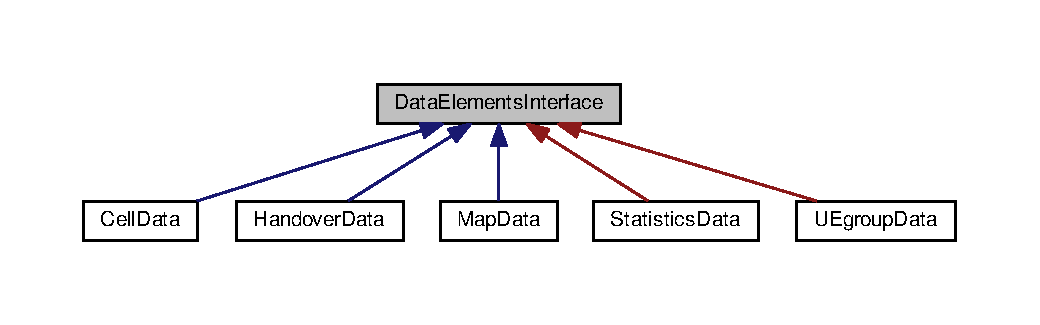
\includegraphics[width=350pt]{class_data_elements_interface__inherit__graph}
\end{center}
\end{figure}
\subsection*{Public Member Functions}
\begin{DoxyCompactItemize}
\item 
virtual Q\+String {\bfseries get\+Element\+Type} () const =0\hypertarget{class_data_elements_interface_ab71fa5312e02fb60413a3d4c716178f5}{}\label{class_data_elements_interface_ab71fa5312e02fb60413a3d4c716178f5}

\item 
virtual void {\bfseries serialize\+To\+Project\+File} ()=0\hypertarget{class_data_elements_interface_aee0663d36996c579b82ae05024176b51}{}\label{class_data_elements_interface_aee0663d36996c579b82ae05024176b51}

\item 
virtual void {\bfseries serialize\+From\+Project\+File\+Old} (Q\+Byte\+Array raw\+Data)=0\hypertarget{class_data_elements_interface_a97c737d424310e61839128253a1af964}{}\label{class_data_elements_interface_a97c737d424310e61839128253a1af964}

\item 
virtual void {\bfseries serialize\+From\+Project\+File\+New} (Q\+Dom\+Document xml\+Document)=0\hypertarget{class_data_elements_interface_aa1d9396933051fb710877078d47c695e}{}\label{class_data_elements_interface_aa1d9396933051fb710877078d47c695e}

\item 
virtual void {\bfseries serialize\+To\+Script\+Commands} ()=0\hypertarget{class_data_elements_interface_aee2fd04decdf32d9e7f98b8458108a24}{}\label{class_data_elements_interface_aee2fd04decdf32d9e7f98b8458108a24}

\end{DoxyCompactItemize}


The documentation for this class was generated from the following file\+:\begin{DoxyCompactItemize}
\item 
/home/trance/\+L\+T\+Esim/\+Internal.\+L\+T\+Esim\+Generator/\+L\+T\+Esim\+Generator\+G\+U\+I/dataelementsinterface.\+h\end{DoxyCompactItemize}

\hypertarget{class_double_input_validator}{}\section{Double\+Input\+Validator Class Reference}
\label{class_double_input_validator}\index{Double\+Input\+Validator@{Double\+Input\+Validator}}


Inheritance diagram for Double\+Input\+Validator\+:
\nopagebreak
\begin{figure}[H]
\begin{center}
\leavevmode
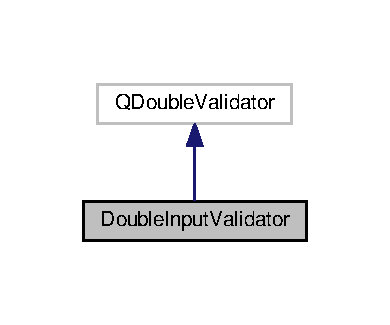
\includegraphics[width=187pt]{class_double_input_validator__inherit__graph}
\end{center}
\end{figure}


Collaboration diagram for Double\+Input\+Validator\+:
\nopagebreak
\begin{figure}[H]
\begin{center}
\leavevmode
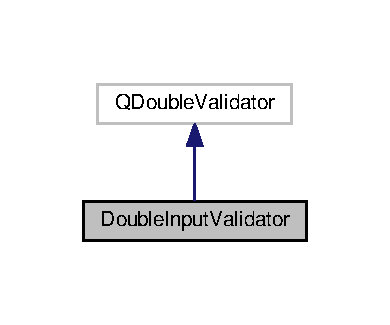
\includegraphics[width=187pt]{class_double_input_validator__coll__graph}
\end{center}
\end{figure}
\subsection*{Public Member Functions}
\begin{DoxyCompactItemize}
\item 
{\bfseries Double\+Input\+Validator} (double bottom, double top, int decimals, Q\+Object $\ast$parent=0)\hypertarget{class_double_input_validator_a6619875c72078f7808e9535740564523}{}\label{class_double_input_validator_a6619875c72078f7808e9535740564523}

\item 
Q\+Validator\+::\+State {\bfseries validate} (Q\+String \&, int \&) const \hypertarget{class_double_input_validator_a653c2af396d2320e9c9f6da34e7f63da}{}\label{class_double_input_validator_a653c2af396d2320e9c9f6da34e7f63da}

\end{DoxyCompactItemize}


The documentation for this class was generated from the following files\+:\begin{DoxyCompactItemize}
\item 
/home/trance/\+L\+T\+Esim/\+Internal.\+L\+T\+Esim\+Generator/\+L\+T\+Esim\+Generator\+G\+U\+I/\+Double\+Input\+Validator/doubleinputvalidator.\+h\item 
/home/trance/\+L\+T\+Esim/\+Internal.\+L\+T\+Esim\+Generator/\+L\+T\+Esim\+Generator\+G\+U\+I/\+Double\+Input\+Validator/doubleinputvalidator.\+cpp\end{DoxyCompactItemize}

\hypertarget{class_drag_u_e_label}{}\section{Drag\+U\+E\+Label Class Reference}
\label{class_drag_u_e_label}\index{Drag\+U\+E\+Label@{Drag\+U\+E\+Label}}


Inheritance diagram for Drag\+U\+E\+Label\+:
\nopagebreak
\begin{figure}[H]
\begin{center}
\leavevmode
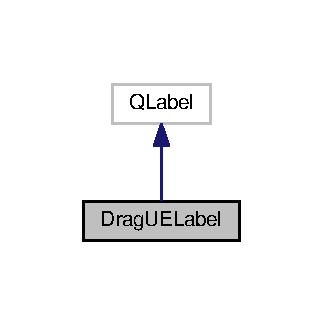
\includegraphics[width=155pt]{class_drag_u_e_label__inherit__graph}
\end{center}
\end{figure}


Collaboration diagram for Drag\+U\+E\+Label\+:
\nopagebreak
\begin{figure}[H]
\begin{center}
\leavevmode
\includegraphics[width=155pt]{class_drag_u_e_label__coll__graph}
\end{center}
\end{figure}
\subsection*{Public Member Functions}
\begin{DoxyCompactItemize}
\item 
{\bfseries Drag\+U\+E\+Label} (const Q\+String \&text, Q\+Widget $\ast$parent=0)\hypertarget{class_drag_u_e_label_a0d91ab68fcf7eef05836beb52fa0aa86}{}\label{class_drag_u_e_label_a0d91ab68fcf7eef05836beb52fa0aa86}

\item 
Q\+String {\bfseries label\+Text} () const \hypertarget{class_drag_u_e_label_a31cf6bfb3c49f8845a25eb2c1a1710b2}{}\label{class_drag_u_e_label_a31cf6bfb3c49f8845a25eb2c1a1710b2}

\item 
void {\bfseries mouse\+Double\+Click\+Event} (Q\+Mouse\+Event $\ast$event)\hypertarget{class_drag_u_e_label_a3c6e6d530c44133e9d4b047001e0192d}{}\label{class_drag_u_e_label_a3c6e6d530c44133e9d4b047001e0192d}

\item 
void {\bfseries setmy\+Area} (\hyperlink{class_my_object_area}{My\+Object\+Area} $\ast$object\+Area)\hypertarget{class_drag_u_e_label_a5438d265f61c4d8955bb02ac77bd2453}{}\label{class_drag_u_e_label_a5438d265f61c4d8955bb02ac77bd2453}

\item 
\hyperlink{class_my_object_area}{My\+Object\+Area} $\ast$ {\bfseries getmy\+Area} ()\hypertarget{class_drag_u_e_label_a368ba405088b1a017d3eb76e026162e0}{}\label{class_drag_u_e_label_a368ba405088b1a017d3eb76e026162e0}

\end{DoxyCompactItemize}
\subsection*{Friends}
\begin{DoxyCompactItemize}
\item 
class {\bfseries Drag\+U\+E\+Label\+\_\+\+Test}\hypertarget{class_drag_u_e_label_a846982edde3dbd494a3dac23b5c9ece7}{}\label{class_drag_u_e_label_a846982edde3dbd494a3dac23b5c9ece7}

\end{DoxyCompactItemize}


The documentation for this class was generated from the following files\+:\begin{DoxyCompactItemize}
\item 
/home/trance/\+L\+T\+Esim/\+Internal.\+L\+T\+Esim\+Generator/\+L\+T\+Esim\+Generator\+G\+U\+I/\+Maps/\+Traffic/\+Map\+Components/draguelabel.\+h\item 
/home/trance/\+L\+T\+Esim/\+Internal.\+L\+T\+Esim\+Generator/\+L\+T\+Esim\+Generator\+G\+U\+I/\+Maps/\+Traffic/\+Map\+Components/draguelabel.\+cpp\end{DoxyCompactItemize}

\hypertarget{class_drag_u_e_label___test}{}\section{Drag\+U\+E\+Label\+\_\+\+Test Class Reference}
\label{class_drag_u_e_label___test}\index{Drag\+U\+E\+Label\+\_\+\+Test@{Drag\+U\+E\+Label\+\_\+\+Test}}


Inheritance diagram for Drag\+U\+E\+Label\+\_\+\+Test\+:
\nopagebreak
\begin{figure}[H]
\begin{center}
\leavevmode
\includegraphics[width=180pt]{class_drag_u_e_label___test__inherit__graph}
\end{center}
\end{figure}


Collaboration diagram for Drag\+U\+E\+Label\+\_\+\+Test\+:
\nopagebreak
\begin{figure}[H]
\begin{center}
\leavevmode
\includegraphics[width=180pt]{class_drag_u_e_label___test__coll__graph}
\end{center}
\end{figure}


The documentation for this class was generated from the following files\+:\begin{DoxyCompactItemize}
\item 
/home/trance/\+L\+T\+Esim/\+Internal.\+L\+T\+Esim\+Generator/\+L\+T\+Esim\+Generator\+G\+U\+I/\+Maps/\+Traffic/\+Map\+Test/\+Map\+Components\+Test/draguelabel\+\_\+test.\+h\item 
/home/trance/\+L\+T\+Esim/\+Internal.\+L\+T\+Esim\+Generator/\+L\+T\+Esim\+Generator\+G\+U\+I/\+Maps/\+Traffic/\+Map\+Test/\+Map\+Components\+Test/draguelabel\+\_\+test.\+cpp\end{DoxyCompactItemize}

\hypertarget{class_form}{}\section{Form Class Reference}
\label{class_form}\index{Form@{Form}}


Inheritance diagram for Form\+:
\nopagebreak
\begin{figure}[H]
\begin{center}
\leavevmode
\includegraphics[width=135pt]{class_form__inherit__graph}
\end{center}
\end{figure}


Collaboration diagram for Form\+:
\nopagebreak
\begin{figure}[H]
\begin{center}
\leavevmode
\includegraphics[width=135pt]{class_form__coll__graph}
\end{center}
\end{figure}
\subsection*{Public Member Functions}
\begin{DoxyCompactItemize}
\item 
{\bfseries Form} (Q\+Widget $\ast$parent=0)\hypertarget{class_form_a9a921e26a02f23bffdea4330d6795796}{}\label{class_form_a9a921e26a02f23bffdea4330d6795796}

\item 
Q\+String {\bfseries get\+\_\+current\+C\+S\+Behavior} ()\hypertarget{class_form_a5323c5653fe4db9957374aa459583aab}{}\label{class_form_a5323c5653fe4db9957374aa459583aab}

\item 
Q\+String {\bfseries get\+\_\+current\+P\+S\+Behavior} ()\hypertarget{class_form_acca8606601f1767d3c65c25c324cb999}{}\label{class_form_acca8606601f1767d3c65c25c324cb999}

\item 
void {\bfseries reset\+Accept} ()\hypertarget{class_form_a4bee5f5335d89623ee9bce9f4fecd607}{}\label{class_form_a4bee5f5335d89623ee9bce9f4fecd607}

\item 
Q\+String {\bfseries get\+\_\+current\+Area} ()\hypertarget{class_form_a1152c1b4a3b711ce4a2b10d3e8a0d823}{}\label{class_form_a1152c1b4a3b711ce4a2b10d3e8a0d823}

\item 
void {\bfseries set\+\_\+current\+Area} (Q\+String value)\hypertarget{class_form_a50f09ab86b91b290cc9ea0d3b1a2eaf6}{}\label{class_form_a50f09ab86b91b290cc9ea0d3b1a2eaf6}

\item 
bool {\bfseries is\+\_\+\+Accepted} ()\hypertarget{class_form_aaf458e32135258145ca010a42cc08a3a}{}\label{class_form_aaf458e32135258145ca010a42cc08a3a}

\item 
Q\+String {\bfseries get\+Window\+Title} ()\hypertarget{class_form_abcb7636415d30c1207c2ab5a4f69c65c}{}\label{class_form_abcb7636415d30c1207c2ab5a4f69c65c}

\item 
void {\bfseries get\+All\+Values} ()\hypertarget{class_form_a17dff1f0df158f6b478441a79d1955b7}{}\label{class_form_a17dff1f0df158f6b478441a79d1955b7}

\item 
Q\+Combo\+Box {\bfseries set\+All\+Values} ()\hypertarget{class_form_a39f20b9caa964df0daeb0aaa71f045b5}{}\label{class_form_a39f20b9caa964df0daeb0aaa71f045b5}

\end{DoxyCompactItemize}
\subsection*{Static Public Member Functions}
\begin{DoxyCompactItemize}
\item 
static int {\bfseries get\+U\+E\+Pairs} ()\hypertarget{class_form_a0450ccaddd3966be1b406167d1133739}{}\label{class_form_a0450ccaddd3966be1b406167d1133739}

\item 
static void {\bfseries reset\+U\+E\+Pairs\+Count} ()\hypertarget{class_form_ad56749806ce3cbddcbbda8c6efc8f79a}{}\label{class_form_ad56749806ce3cbddcbbda8c6efc8f79a}

\end{DoxyCompactItemize}
\subsection*{Public Attributes}
\begin{DoxyCompactItemize}
\item 
Q\+Line\+Edit $\ast$ {\bfseries area1}\hypertarget{class_form_aa6fff22a43be8b373d6a645a98b2a552}{}\label{class_form_aa6fff22a43be8b373d6a645a98b2a552}

\item 
Q\+Line\+Edit $\ast$ {\bfseries area2}\hypertarget{class_form_ae314659e50fb228cf30b9190bba945f2}{}\label{class_form_ae314659e50fb228cf30b9190bba945f2}

\item 
Q\+Combo\+Box $\ast$ {\bfseries pointer\+PS}\hypertarget{class_form_a58bdc0004144ecbd0cee33ae2a5b00c8}{}\label{class_form_a58bdc0004144ecbd0cee33ae2a5b00c8}

\item 
Q\+Widget $\ast$ {\bfseries pointer\+Win\+Title}\hypertarget{class_form_ab5ee7645699f72aa22d1787434f6b647}{}\label{class_form_ab5ee7645699f72aa22d1787434f6b647}

\item 
Q\+Widget $\ast$ {\bfseries pointer\+Win\+Title\+\_\+large}\hypertarget{class_form_ae745c744f4244f8a33ac804c8028af7d}{}\label{class_form_ae745c744f4244f8a33ac804c8028af7d}

\item 
Q\+Combo\+Box $\ast$ {\bfseries combo}\hypertarget{class_form_a8b03dc7e2564f1aeb7b0eb688f0e0655}{}\label{class_form_a8b03dc7e2564f1aeb7b0eb688f0e0655}

\end{DoxyCompactItemize}


The documentation for this class was generated from the following files\+:\begin{DoxyCompactItemize}
\item 
/home/trance/\+L\+T\+Esim/\+Internal.\+L\+T\+Esim\+Generator/\+L\+T\+Esim\+Generator\+G\+U\+I/\+Maps/\+Traffic/\+Ue\+Parameters/U\+E\+\_\+param\+\_\+form.\+h\item 
/home/trance/\+L\+T\+Esim/\+Internal.\+L\+T\+Esim\+Generator/\+L\+T\+Esim\+Generator\+G\+U\+I/\+Maps/\+Traffic/\+Ue\+Parameters/U\+E\+\_\+param\+\_\+form.\+cpp\end{DoxyCompactItemize}

\hypertarget{class_handover}{}\section{Handover Class Reference}
\label{class_handover}\index{Handover@{Handover}}
\subsection*{Public Member Functions}
\begin{DoxyCompactItemize}
\item 
{\bfseries Handover} (Q\+String name)\hypertarget{class_handover_a3968494fea0cf12ab6d434873ccf2e4a}{}\label{class_handover_a3968494fea0cf12ab6d434873ccf2e4a}

\item 
Q\+String {\bfseries get\+Area} ()\hypertarget{class_handover_a35fd85a91c585d59ad571e3868ac1a3c}{}\label{class_handover_a35fd85a91c585d59ad571e3868ac1a3c}

\item 
Q\+String {\bfseries get\+South\+Boundary} ()\hypertarget{class_handover_aff7ba9e3b157a4de64f5eb0e989cf963}{}\label{class_handover_aff7ba9e3b157a4de64f5eb0e989cf963}

\item 
Q\+String {\bfseries get\+North\+Boundary} ()\hypertarget{class_handover_a6a3781fc668d75b1fb9e94ee6e34b1b2}{}\label{class_handover_a6a3781fc668d75b1fb9e94ee6e34b1b2}

\item 
Q\+String {\bfseries get\+West\+Boundary} ()\hypertarget{class_handover_ac9d0ef7aafbce56b0c18df58a8601067}{}\label{class_handover_ac9d0ef7aafbce56b0c18df58a8601067}

\item 
Q\+String {\bfseries get\+East\+Boundary} ()\hypertarget{class_handover_a8d111e4e364c16198889586fb9c619c4}{}\label{class_handover_a8d111e4e364c16198889586fb9c619c4}

\item 
void {\bfseries set\+South\+Boundary} (Q\+String s)\hypertarget{class_handover_afa126987496abe80cbb6de8c16d28be3}{}\label{class_handover_afa126987496abe80cbb6de8c16d28be3}

\item 
void {\bfseries set\+North\+Boundary} (Q\+String n)\hypertarget{class_handover_aa77c9c5f2fb7f665a425599296fe4747}{}\label{class_handover_aa77c9c5f2fb7f665a425599296fe4747}

\item 
void {\bfseries set\+West\+Boundary} (Q\+String w)\hypertarget{class_handover_abe83ab4ff5cf62db95d843042a1eb4aa}{}\label{class_handover_abe83ab4ff5cf62db95d843042a1eb4aa}

\item 
void {\bfseries set\+East\+Boundary} (Q\+String e)\hypertarget{class_handover_a51f980ff22aaf1ba1ec61e8a47f12bf9}{}\label{class_handover_a51f980ff22aaf1ba1ec61e8a47f12bf9}

\item 
void {\bfseries reset\+Params} ()\hypertarget{class_handover_a4fa83bf8e6dfc62c847505f776cc044b}{}\label{class_handover_a4fa83bf8e6dfc62c847505f776cc044b}

\end{DoxyCompactItemize}


The documentation for this class was generated from the following files\+:\begin{DoxyCompactItemize}
\item 
/home/trance/\+L\+T\+Esim/\+Internal.\+L\+T\+Esim\+Generator/\+L\+T\+Esim\+Generator\+G\+U\+I/\+Maps/\+Map\+Objects/handover.\+h\item 
/home/trance/\+L\+T\+Esim/\+Internal.\+L\+T\+Esim\+Generator/\+L\+T\+Esim\+Generator\+G\+U\+I/\+Maps/\+Map\+Objects/handover.\+cpp\end{DoxyCompactItemize}

\hypertarget{class_handover_area}{}\section{Handover\+Area Class Reference}
\label{class_handover_area}\index{Handover\+Area@{Handover\+Area}}


Inheritance diagram for Handover\+Area\+:
\nopagebreak
\begin{figure}[H]
\begin{center}
\leavevmode
\includegraphics[width=159pt]{class_handover_area__inherit__graph}
\end{center}
\end{figure}


Collaboration diagram for Handover\+Area\+:
\nopagebreak
\begin{figure}[H]
\begin{center}
\leavevmode
\includegraphics[width=159pt]{class_handover_area__coll__graph}
\end{center}
\end{figure}
\subsection*{Public Member Functions}
\begin{DoxyCompactItemize}
\item 
{\bfseries Handover\+Area} (\hyperlink{class_cell_area}{Cell\+Area} $\ast$cell1, \hyperlink{class_cell_area}{Cell\+Area} $\ast$cell2)\hypertarget{class_handover_area_a7beacdf5ff05d71038ddb261cc3cc2b7}{}\label{class_handover_area_a7beacdf5ff05d71038ddb261cc3cc2b7}

\item 
bool {\bfseries contain} (int x\+Pos, int y\+Pos, \hyperlink{class_my_object_area}{My\+Object\+Area} $\ast$$\ast$obj\+Ptr1)\hypertarget{class_handover_area_a3d8ea54fcc430d95073069553cdec841}{}\label{class_handover_area_a3d8ea54fcc430d95073069553cdec841}

\item 
Q\+String {\bfseries get\+ID} ()\hypertarget{class_handover_area_a6fffef300bed7a47bcdd5e96b070dda3}{}\label{class_handover_area_a6fffef300bed7a47bcdd5e96b070dda3}

\end{DoxyCompactItemize}


The documentation for this class was generated from the following files\+:\begin{DoxyCompactItemize}
\item 
/home/trance/\+L\+T\+Esim/\+Internal.\+L\+T\+Esim\+Generator/\+L\+T\+Esim\+Generator\+G\+U\+I/\+Maps/\+Traffic/\+Map\+Components/handoverarea.\+h\item 
/home/trance/\+L\+T\+Esim/\+Internal.\+L\+T\+Esim\+Generator/\+L\+T\+Esim\+Generator\+G\+U\+I/\+Maps/\+Traffic/\+Map\+Components/handoverarea.\+cpp\end{DoxyCompactItemize}

\hypertarget{class_handover_area___test}{}\section{Handover\+Area\+\_\+\+Test Class Reference}
\label{class_handover_area___test}\index{Handover\+Area\+\_\+\+Test@{Handover\+Area\+\_\+\+Test}}


Inheritance diagram for Handover\+Area\+\_\+\+Test\+:
\nopagebreak
\begin{figure}[H]
\begin{center}
\leavevmode
\includegraphics[width=184pt]{class_handover_area___test__inherit__graph}
\end{center}
\end{figure}


Collaboration diagram for Handover\+Area\+\_\+\+Test\+:
\nopagebreak
\begin{figure}[H]
\begin{center}
\leavevmode
\includegraphics[width=184pt]{class_handover_area___test__coll__graph}
\end{center}
\end{figure}


The documentation for this class was generated from the following files\+:\begin{DoxyCompactItemize}
\item 
/home/trance/\+L\+T\+Esim/\+Internal.\+L\+T\+Esim\+Generator/\+L\+T\+Esim\+Generator\+G\+U\+I/\+Maps/\+Traffic/\+Map\+Test/\+Map\+Components\+Test/handoverarea\+\_\+test.\+h\item 
/home/trance/\+L\+T\+Esim/\+Internal.\+L\+T\+Esim\+Generator/\+L\+T\+Esim\+Generator\+G\+U\+I/\+Maps/\+Traffic/\+Map\+Test/\+Map\+Components\+Test/handoverarea\+\_\+test.\+cpp\end{DoxyCompactItemize}

\hypertarget{class_handover_data}{}\section{Handover\+Data Class Reference}
\label{class_handover_data}\index{Handover\+Data@{Handover\+Data}}


Inheritance diagram for Handover\+Data\+:
\nopagebreak
\begin{figure}[H]
\begin{center}
\leavevmode
\includegraphics[width=197pt]{class_handover_data__inherit__graph}
\end{center}
\end{figure}


Collaboration diagram for Handover\+Data\+:
\nopagebreak
\begin{figure}[H]
\begin{center}
\leavevmode
\includegraphics[width=197pt]{class_handover_data__coll__graph}
\end{center}
\end{figure}
\subsection*{Public Member Functions}
\begin{DoxyCompactItemize}
\item 
{\bfseries Handover\+Data} (Q\+String name, \hyperlink{class_app_settings}{App\+Settings} $\ast$app\+Settings)\hypertarget{class_handover_data_a0ebdcdf3e6e19113905b1d5d012f6a0b}{}\label{class_handover_data_a0ebdcdf3e6e19113905b1d5d012f6a0b}

\item 
Q\+String {\bfseries get\+Handover\+Name} () const \hypertarget{class_handover_data_afc88231951f57e84f261d0f29f9ed761}{}\label{class_handover_data_afc88231951f57e84f261d0f29f9ed761}

\item 
int {\bfseries get\+South\+Boundary} () const \hypertarget{class_handover_data_aa7240bb71bd2b3f13ab0f4ff00c1c779}{}\label{class_handover_data_aa7240bb71bd2b3f13ab0f4ff00c1c779}

\item 
int {\bfseries get\+North\+Boundary} () const \hypertarget{class_handover_data_a3b68a3562f9c37188b21eee29ba3f9a7}{}\label{class_handover_data_a3b68a3562f9c37188b21eee29ba3f9a7}

\item 
int {\bfseries get\+West\+Boundary} () const \hypertarget{class_handover_data_aadcfee4d7b0c6c4091c913f4da6997de}{}\label{class_handover_data_aadcfee4d7b0c6c4091c913f4da6997de}

\item 
int {\bfseries get\+East\+Boundary} () const \hypertarget{class_handover_data_afb7972ace81cf60fc32e91d94f276c1b}{}\label{class_handover_data_afb7972ace81cf60fc32e91d94f276c1b}

\item 
\hyperlink{struct_handover_params}{Handover\+Params} {\bfseries get\+Handover\+Params} () const \hypertarget{class_handover_data_a2d2c8f3f0865c5d97e2f6cca132db310}{}\label{class_handover_data_a2d2c8f3f0865c5d97e2f6cca132db310}

\item 
void {\bfseries set\+Handover\+Name} (const Q\+String \&name)\hypertarget{class_handover_data_aa2ebdd4cdea80d68d74ed11e76ab7b5d}{}\label{class_handover_data_aa2ebdd4cdea80d68d74ed11e76ab7b5d}

\item 
void {\bfseries set\+South\+Boundary} (int south)\hypertarget{class_handover_data_a7206dedee68b4bb70a65f561bf499e5c}{}\label{class_handover_data_a7206dedee68b4bb70a65f561bf499e5c}

\item 
void {\bfseries set\+North\+Boundary} (int north)\hypertarget{class_handover_data_a0c8a86e0349737f35ccf1bb6d76badd7}{}\label{class_handover_data_a0c8a86e0349737f35ccf1bb6d76badd7}

\item 
void {\bfseries set\+West\+Boundary} (int west)\hypertarget{class_handover_data_a58e774266ed7cea002d2e2ceb282ede0}{}\label{class_handover_data_a58e774266ed7cea002d2e2ceb282ede0}

\item 
void {\bfseries set\+East\+Boundary} (int east)\hypertarget{class_handover_data_a4821fcb178c67fcac39c865fe4d02fdc}{}\label{class_handover_data_a4821fcb178c67fcac39c865fe4d02fdc}

\item 
void {\bfseries set\+Handover\+Params} (const \hyperlink{struct_handover_params}{Handover\+Params} \&params)\hypertarget{class_handover_data_a44bf5aeb9853496e72cfbdcd1be5de3f}{}\label{class_handover_data_a44bf5aeb9853496e72cfbdcd1be5de3f}

\item 
\hyperlink{struct_handover_params}{Handover\+Params} {\bfseries parse\+Data\+From\+List} (Q\+String\+List \&params\+List)\hypertarget{class_handover_data_a8e27ad24e6f78a36e80c68b0e2c8a245}{}\label{class_handover_data_a8e27ad24e6f78a36e80c68b0e2c8a245}

\item 
Q\+String {\bfseries get\+Element\+Type} () const override\hypertarget{class_handover_data_a4e1386200bc54a49a967963baeb0c049}{}\label{class_handover_data_a4e1386200bc54a49a967963baeb0c049}

\item 
void {\bfseries serialize\+To\+Project\+File} () override\hypertarget{class_handover_data_a45511d327dbabba83a3e2699012e9336}{}\label{class_handover_data_a45511d327dbabba83a3e2699012e9336}

\item 
void {\bfseries serialize\+From\+Project\+File\+Old} (Q\+Byte\+Array raw\+Data) override\hypertarget{class_handover_data_a710b11d41d03255073c5bcf50ca96ed7}{}\label{class_handover_data_a710b11d41d03255073c5bcf50ca96ed7}

\item 
void {\bfseries serialize\+From\+Project\+File\+New} (Q\+Dom\+Document xml\+Document) override\hypertarget{class_handover_data_ad7aea1441cddf5f6fba5809685da7ad7}{}\label{class_handover_data_ad7aea1441cddf5f6fba5809685da7ad7}

\item 
void {\bfseries serialize\+To\+Script\+Commands} () override\hypertarget{class_handover_data_a1f38a95529d4c5e791a9749e796fcc44}{}\label{class_handover_data_a1f38a95529d4c5e791a9749e796fcc44}

\item 
void {\bfseries set\+Project\+Reader\+Writer} (\hyperlink{class_project_reader_writer}{Project\+Reader\+Writer} $\ast$value)\hypertarget{class_handover_data_a7ff75a2bc77e7d610c52180ce3288ef8}{}\label{class_handover_data_a7ff75a2bc77e7d610c52180ce3288ef8}

\end{DoxyCompactItemize}


The documentation for this class was generated from the following files\+:\begin{DoxyCompactItemize}
\item 
/home/trance/\+L\+T\+Esim/\+Internal.\+L\+T\+Esim\+Generator/\+L\+T\+Esim\+Generator\+G\+U\+I/\+Maps/\+Traffic/\+Data\+Objects/handoverdata.\+h\item 
/home/trance/\+L\+T\+Esim/\+Internal.\+L\+T\+Esim\+Generator/\+L\+T\+Esim\+Generator\+G\+U\+I/\+Maps/\+Traffic/\+Data\+Objects/handoverdata.\+cpp\end{DoxyCompactItemize}

\hypertarget{class_handover_data___test}{}\section{Handover\+Data\+\_\+\+Test Class Reference}
\label{class_handover_data___test}\index{Handover\+Data\+\_\+\+Test@{Handover\+Data\+\_\+\+Test}}


Inheritance diagram for Handover\+Data\+\_\+\+Test\+:
\nopagebreak
\begin{figure}[H]
\begin{center}
\leavevmode
\includegraphics[width=184pt]{class_handover_data___test__inherit__graph}
\end{center}
\end{figure}


Collaboration diagram for Handover\+Data\+\_\+\+Test\+:
\nopagebreak
\begin{figure}[H]
\begin{center}
\leavevmode
\includegraphics[width=244pt]{class_handover_data___test__coll__graph}
\end{center}
\end{figure}
\subsection*{Public Member Functions}
\begin{DoxyCompactItemize}
\item 
{\bfseries Handover\+Data\+\_\+\+Test} (\hyperlink{class_app_settings}{App\+Settings} $\ast$app\+Settings, Q\+Object $\ast$parent=0)\hypertarget{class_handover_data___test_a0017ba4b1d791d631412d057ce0936be}{}\label{class_handover_data___test_a0017ba4b1d791d631412d057ce0936be}

\item 
void {\bfseries set\+Project\+Reader\+Writer} (\hyperlink{class_project_reader_writer}{Project\+Reader\+Writer} $\ast$value)\hypertarget{class_handover_data___test_a6d191ea39d2691b05a69f9319a9307eb}{}\label{class_handover_data___test_a6d191ea39d2691b05a69f9319a9307eb}

\end{DoxyCompactItemize}
\subsection*{Public Attributes}
\begin{DoxyCompactItemize}
\item 
Q\+String {\bfseries handover\+Name1} = \char`\"{}Handover11\+\_\+21\char`\"{}\hypertarget{class_handover_data___test_ac50018bf1c091fab93c6eabe9b09ab30}{}\label{class_handover_data___test_ac50018bf1c091fab93c6eabe9b09ab30}

\item 
Q\+String {\bfseries handover\+Name2} = \char`\"{}Handover21\+\_\+22\char`\"{}\hypertarget{class_handover_data___test_a1cef767b4374585c6bdc612a24cad021}{}\label{class_handover_data___test_a1cef767b4374585c6bdc612a24cad021}

\item 
Q\+String {\bfseries test\+Operators\+File} = \char`\"{}operators\char`\"{}\hypertarget{class_handover_data___test_a9aa22d6bbdaf5c780a2a72882ed69a27}{}\label{class_handover_data___test_a9aa22d6bbdaf5c780a2a72882ed69a27}

\item 
Q\+String {\bfseries test\+Project\+Name} = \char`\"{}test\char`\"{}\hypertarget{class_handover_data___test_acee03177b190c2de467e0283de8bde86}{}\label{class_handover_data___test_acee03177b190c2de467e0283de8bde86}

\item 
Q\+String {\bfseries test\+Project\+Dir} = \char`\"{}projects\char`\"{}\hypertarget{class_handover_data___test_a35ec0bc1c07c5a5120bc59cc3cf99c45}{}\label{class_handover_data___test_a35ec0bc1c07c5a5120bc59cc3cf99c45}

\item 
\hyperlink{struct_handover_params}{Handover\+Params} {\bfseries test\+Params}\hypertarget{class_handover_data___test_aa581126ae6478661e3e01037ed07301b}{}\label{class_handover_data___test_aa581126ae6478661e3e01037ed07301b}

\item 
const char $\ast$ {\bfseries test\+Phrase} = \char`\"{}Handover11\+\_\+12\char`\"{}\hypertarget{class_handover_data___test_a7191a3fb1fd66b6c065854bed04992d8}{}\label{class_handover_data___test_a7191a3fb1fd66b6c065854bed04992d8}

\item 
int {\bfseries test\+Number} = 7750\hypertarget{class_handover_data___test_a95bf3f94c2823b09376499b6122fe7f4}{}\label{class_handover_data___test_a95bf3f94c2823b09376499b6122fe7f4}

\end{DoxyCompactItemize}


The documentation for this class was generated from the following files\+:\begin{DoxyCompactItemize}
\item 
/home/trance/\+L\+T\+Esim/\+Internal.\+L\+T\+Esim\+Generator/\+L\+T\+Esim\+Generator\+G\+U\+I/\+Maps/\+Traffic/\+Map\+Test/\+Data\+Objects\+Test/\+Handover\+Data\+Test/handoverdata\+\_\+test.\+h\item 
/home/trance/\+L\+T\+Esim/\+Internal.\+L\+T\+Esim\+Generator/\+L\+T\+Esim\+Generator\+G\+U\+I/\+Maps/\+Traffic/\+Map\+Test/\+Data\+Objects\+Test/\+Handover\+Data\+Test/handoverdata\+\_\+test.\+cpp\end{DoxyCompactItemize}

\hypertarget{structhandover_name}{}\section{handover\+Name Struct Reference}
\label{structhandover_name}\index{handover\+Name@{handover\+Name}}


Collaboration diagram for handover\+Name\+:
\nopagebreak
\begin{figure}[H]
\begin{center}
\leavevmode
\includegraphics[width=163pt]{structhandover_name__coll__graph}
\end{center}
\end{figure}
\subsection*{Public Attributes}
\begin{DoxyCompactItemize}
\item 
\hyperlink{class_handover}{Handover} $\ast$ {\bfseries obj}\hypertarget{structhandover_name_a5626a26d3d1c5b2cba3e2ef32dccef74}{}\label{structhandover_name_a5626a26d3d1c5b2cba3e2ef32dccef74}

\item 
Q\+String {\bfseries name}\hypertarget{structhandover_name_a3a66e14c88f16e5bdbda04bfba71e361}{}\label{structhandover_name_a3a66e14c88f16e5bdbda04bfba71e361}

\end{DoxyCompactItemize}


The documentation for this struct was generated from the following file\+:\begin{DoxyCompactItemize}
\item 
/home/trance/\+L\+T\+Esim/\+Internal.\+L\+T\+Esim\+Generator/\+L\+T\+Esim\+Generator\+G\+U\+I/\+Management\+Window/\+Encryption/encryption.\+h\end{DoxyCompactItemize}

\hypertarget{struct_handover_params}{}\section{Handover\+Params Struct Reference}
\label{struct_handover_params}\index{Handover\+Params@{Handover\+Params}}
\subsection*{Public Attributes}
\begin{DoxyCompactItemize}
\item 
Q\+String {\bfseries handover\+Name}\hypertarget{struct_handover_params_aeffdfac83dad11bd194b0840aee85280}{}\label{struct_handover_params_aeffdfac83dad11bd194b0840aee85280}

\item 
Q\+Rect {\bfseries handover\+Area}\hypertarget{struct_handover_params_a3b6ca35a4d4eb3441766dd0cb8f2e13b}{}\label{struct_handover_params_a3b6ca35a4d4eb3441766dd0cb8f2e13b}

\end{DoxyCompactItemize}


The documentation for this struct was generated from the following file\+:\begin{DoxyCompactItemize}
\item 
/home/trance/\+L\+T\+Esim/\+Internal.\+L\+T\+Esim\+Generator/\+L\+T\+Esim\+Generator\+G\+U\+I/\+Maps/\+Traffic/\+Data\+Objects/handoverdata.\+h\end{DoxyCompactItemize}

\hypertarget{class_help_dialog}{}\section{Help\+Dialog Class Reference}
\label{class_help_dialog}\index{Help\+Dialog@{Help\+Dialog}}


Inheritance diagram for Help\+Dialog\+:
\nopagebreak
\begin{figure}[H]
\begin{center}
\leavevmode
\includegraphics[width=145pt]{class_help_dialog__inherit__graph}
\end{center}
\end{figure}


Collaboration diagram for Help\+Dialog\+:
\nopagebreak
\begin{figure}[H]
\begin{center}
\leavevmode
\includegraphics[width=145pt]{class_help_dialog__coll__graph}
\end{center}
\end{figure}
\subsection*{Public Member Functions}
\begin{DoxyCompactItemize}
\item 
{\bfseries Help\+Dialog} (Q\+Widget $\ast$parent=0)\hypertarget{class_help_dialog_ab2cdaaff98141da0157b317e8a233e0f}{}\label{class_help_dialog_ab2cdaaff98141da0157b317e8a233e0f}

\end{DoxyCompactItemize}


The documentation for this class was generated from the following files\+:\begin{DoxyCompactItemize}
\item 
/home/trance/\+L\+T\+Esim/\+Internal.\+L\+T\+Esim\+Generator/\+L\+T\+Esim\+Generator\+G\+U\+I/\+Management\+Window/\+Helpdialog/helpdialog.\+h\item 
/home/trance/\+L\+T\+Esim/\+Internal.\+L\+T\+Esim\+Generator/\+L\+T\+Esim\+Generator\+G\+U\+I/\+Management\+Window/\+Helpdialog/helpdialog.\+cpp\end{DoxyCompactItemize}

\hypertarget{classipex_form}{}\section{ipex\+Form Class Reference}
\label{classipex_form}\index{ipex\+Form@{ipex\+Form}}


Inheritance diagram for ipex\+Form\+:
\nopagebreak
\begin{figure}[H]
\begin{center}
\leavevmode
\includegraphics[width=137pt]{classipex_form__inherit__graph}
\end{center}
\end{figure}


Collaboration diagram for ipex\+Form\+:
\nopagebreak
\begin{figure}[H]
\begin{center}
\leavevmode
\includegraphics[width=137pt]{classipex_form__coll__graph}
\end{center}
\end{figure}
\subsection*{Public Member Functions}
\begin{DoxyCompactItemize}
\item 
{\bfseries ipex\+Form} (Q\+Widget $\ast$parent=0)\hypertarget{classipex_form_a74d570ebd91e0215f3ca0abf4db58c79}{}\label{classipex_form_a74d570ebd91e0215f3ca0abf4db58c79}

\item 
void {\bfseries set\+\_\+checkboxactive} (bool check)\hypertarget{classipex_form_a574dabff8ac846ba7e6551795b6ee5ef}{}\label{classipex_form_a574dabff8ac846ba7e6551795b6ee5ef}

\item 
bool {\bfseries get\+\_\+checkboxactive} ()\hypertarget{classipex_form_aacc1ae0386bf54465506f575f804e1ca}{}\label{classipex_form_aacc1ae0386bf54465506f575f804e1ca}

\item 
void {\bfseries set\+Parameters} (\hyperlink{class_ipgwtg}{Ipgwtg} $\ast$ipex, bool flag\+Ue)\hypertarget{classipex_form_abe10f0dd8d705a043eb1b553309b85e9}{}\label{classipex_form_abe10f0dd8d705a043eb1b553309b85e9}

\end{DoxyCompactItemize}


The documentation for this class was generated from the following files\+:\begin{DoxyCompactItemize}
\item 
/home/trance/\+L\+T\+Esim/\+Internal.\+L\+T\+Esim\+Generator/\+L\+T\+Esim\+Generator\+G\+U\+I/\+Maps/\+Parameters/\+Simulated\+Ue/ipexform.\+h\item 
/home/trance/\+L\+T\+Esim/\+Internal.\+L\+T\+Esim\+Generator/\+L\+T\+Esim\+Generator\+G\+U\+I/\+Maps/\+Parameters/\+Simulated\+Ue/ipexform.\+cpp\end{DoxyCompactItemize}

\hypertarget{class_ipgwtg}{}\section{Ipgwtg Class Reference}
\label{class_ipgwtg}\index{Ipgwtg@{Ipgwtg}}
\subsection*{Public Member Functions}
\begin{DoxyCompactItemize}
\item 
Q\+String {\bfseries get\+Data\+Generator} ()\hypertarget{class_ipgwtg_ac2969f232fdf68afcbc425bfe2ba7143}{}\label{class_ipgwtg_ac2969f232fdf68afcbc425bfe2ba7143}

\item 
void {\bfseries set\+Data\+Generator} (Q\+String value)\hypertarget{class_ipgwtg_aac7cd5164f56ae4dff017e5c9455882b}{}\label{class_ipgwtg_aac7cd5164f56ae4dff017e5c9455882b}

\item 
Q\+String {\bfseries get\+User\+Data\+Gen} ()\hypertarget{class_ipgwtg_a139f41974c4ba9870fcd1e5b380e8a83}{}\label{class_ipgwtg_a139f41974c4ba9870fcd1e5b380e8a83}

\item 
void {\bfseries set\+User\+Data\+Gen} (Q\+String value)\hypertarget{class_ipgwtg_a1f7de2a388ba30606371c646a93256d7}{}\label{class_ipgwtg_a1f7de2a388ba30606371c646a93256d7}

\item 
bool {\bfseries get\+Start\+\_\+isp\+\_\+simulator} () const \hypertarget{class_ipgwtg_ad38db27c6597f5f75e3b2ffbe2358690}{}\label{class_ipgwtg_ad38db27c6597f5f75e3b2ffbe2358690}

\item 
void {\bfseries set\+Start\+\_\+isp\+\_\+simulator} (bool value)\hypertarget{class_ipgwtg_adbd149bdef5a48283a089839e7022ef8}{}\label{class_ipgwtg_adbd149bdef5a48283a089839e7022ef8}

\item 
Q\+String {\bfseries get\+Ipgwtg\+\_\+ip\+Address} ()\hypertarget{class_ipgwtg_aff9e01b6f4334ed47be80e0fcaffae8e}{}\label{class_ipgwtg_aff9e01b6f4334ed47be80e0fcaffae8e}

\item 
void {\bfseries set\+Ipgwtg\+\_\+ip\+Address} (Q\+String value)\hypertarget{class_ipgwtg_a60e773b6803400d5de6ac9c3beac0d41}{}\label{class_ipgwtg_a60e773b6803400d5de6ac9c3beac0d41}

\item 
bool {\bfseries get\+Ipgwtg\+\_\+inband\+\_\+signaling} () const \hypertarget{class_ipgwtg_a5a61750df10775fd63dc0768cc236c9b}{}\label{class_ipgwtg_a5a61750df10775fd63dc0768cc236c9b}

\item 
void {\bfseries set\+Ipgwtg\+\_\+inband\+\_\+signaling} (bool value)\hypertarget{class_ipgwtg_a6ad972a01432e0522fd940194d25a565}{}\label{class_ipgwtg_a6ad972a01432e0522fd940194d25a565}

\item 
Q\+String {\bfseries get\+Ipgwtg\+\_\+port} () const \hypertarget{class_ipgwtg_a6cc81fad79ad64fc333ca506ab9f502f}{}\label{class_ipgwtg_a6cc81fad79ad64fc333ca506ab9f502f}

\item 
void {\bfseries set\+Ipgwtg\+\_\+port} (Q\+String value)\hypertarget{class_ipgwtg_a38cff1ebac489798a39de859f3307583}{}\label{class_ipgwtg_a38cff1ebac489798a39de859f3307583}

\item 
bool {\bfseries get\+Ipgwtg\+\_\+ftp\+\_\+sender\+\_\+connect\+\_\+put} () const \hypertarget{class_ipgwtg_a72d96afffb776b93f1ddfb89bc94b94c}{}\label{class_ipgwtg_a72d96afffb776b93f1ddfb89bc94b94c}

\item 
void {\bfseries set\+Ipgwtg\+\_\+ftp\+\_\+sender\+\_\+connect\+\_\+put} (bool value)\hypertarget{class_ipgwtg_a042398e1cdb462226011faf2e33b81f6}{}\label{class_ipgwtg_a042398e1cdb462226011faf2e33b81f6}

\item 
void {\bfseries reset\+Params} ()\hypertarget{class_ipgwtg_ab948dc90a12144e4b4fd031a3fdb7d89}{}\label{class_ipgwtg_ab948dc90a12144e4b4fd031a3fdb7d89}

\end{DoxyCompactItemize}


The documentation for this class was generated from the following files\+:\begin{DoxyCompactItemize}
\item 
/home/trance/\+L\+T\+Esim/\+Internal.\+L\+T\+Esim\+Generator/\+L\+T\+Esim\+Generator\+G\+U\+I/\+Maps/\+Parameters/\+Simulated\+Ue/ipgwtg.\+h\item 
/home/trance/\+L\+T\+Esim/\+Internal.\+L\+T\+Esim\+Generator/\+L\+T\+Esim\+Generator\+G\+U\+I/\+Maps/\+Parameters/\+Simulated\+Ue/ipgwtg.\+cpp\end{DoxyCompactItemize}

\hypertarget{class_management_template}{}\section{Management\+Template Class Reference}
\label{class_management_template}\index{Management\+Template@{Management\+Template}}


Inheritance diagram for Management\+Template\+:
\nopagebreak
\begin{figure}[H]
\begin{center}
\leavevmode
\includegraphics[width=193pt]{class_management_template__inherit__graph}
\end{center}
\end{figure}


Collaboration diagram for Management\+Template\+:
\nopagebreak
\begin{figure}[H]
\begin{center}
\leavevmode
\includegraphics[width=193pt]{class_management_template__coll__graph}
\end{center}
\end{figure}
\subsection*{Public Member Functions}
\begin{DoxyCompactItemize}
\item 
{\bfseries Management\+Template} (Q\+Widget $\ast$parent=0)\hypertarget{class_management_template_ad31491b5f974a7284e5b8f8c8251291a}{}\label{class_management_template_ad31491b5f974a7284e5b8f8c8251291a}

\end{DoxyCompactItemize}
\subsection*{Public Attributes}
\begin{DoxyCompactItemize}
\item 
Ui\+::\+Management\+Template $\ast$ {\bfseries ui}\hypertarget{class_management_template_a268eb55ab2663faa9f9c384836dfcc00}{}\label{class_management_template_a268eb55ab2663faa9f9c384836dfcc00}

\end{DoxyCompactItemize}
\subsection*{Protected Attributes}
\begin{DoxyCompactItemize}
\item 
Q\+Push\+Button $\ast$ {\bfseries save\+Button}\hypertarget{class_management_template_ade2765de8ddd0253d2b3bf866b4dc7d3}{}\label{class_management_template_ade2765de8ddd0253d2b3bf866b4dc7d3}

\item 
Q\+Push\+Button $\ast$ {\bfseries cancel\+Button}\hypertarget{class_management_template_a558f7f32407736630f2c79e32c231f28}{}\label{class_management_template_a558f7f32407736630f2c79e32c231f28}

\end{DoxyCompactItemize}


The documentation for this class was generated from the following files\+:\begin{DoxyCompactItemize}
\item 
/home/trance/\+L\+T\+Esim/\+Internal.\+L\+T\+Esim\+Generator/\+L\+T\+Esim\+Generator\+G\+U\+I/\+Maps/\+Traffic/\+Management\+Template/managementtemplate.\+h\item 
/home/trance/\+L\+T\+Esim/\+Internal.\+L\+T\+Esim\+Generator/\+L\+T\+Esim\+Generator\+G\+U\+I/\+Maps/\+Traffic/\+Management\+Template/managementtemplate.\+cpp\end{DoxyCompactItemize}

\hypertarget{class_management_template___test}{}\section{Management\+Template\+\_\+\+Test Class Reference}
\label{class_management_template___test}\index{Management\+Template\+\_\+\+Test@{Management\+Template\+\_\+\+Test}}


Inheritance diagram for Management\+Template\+\_\+\+Test\+:
\nopagebreak
\begin{figure}[H]
\begin{center}
\leavevmode
\includegraphics[width=218pt]{class_management_template___test__inherit__graph}
\end{center}
\end{figure}


Collaboration diagram for Management\+Template\+\_\+\+Test\+:
\nopagebreak
\begin{figure}[H]
\begin{center}
\leavevmode
\includegraphics[width=294pt]{class_management_template___test__coll__graph}
\end{center}
\end{figure}
\subsection*{Public Member Functions}
\begin{DoxyCompactItemize}
\item 
{\bfseries Management\+Template\+\_\+\+Test} (\hyperlink{class_management_template}{Management\+Template} \&arg\+Management\+Template)\hypertarget{class_management_template___test_a4c6f8a0f1e5748aace7197a414a56720}{}\label{class_management_template___test_a4c6f8a0f1e5748aace7197a414a56720}

\end{DoxyCompactItemize}
\subsection*{Public Attributes}
\begin{DoxyCompactItemize}
\item 
\hyperlink{class_management_template}{Management\+Template} $\ast$ {\bfseries management\+Template}\hypertarget{class_management_template___test_a4dd412a3e97b9e85bf984d02fdd60b30}{}\label{class_management_template___test_a4dd412a3e97b9e85bf984d02fdd60b30}

\item 
\hyperlink{class_management_template}{Management\+Template} $\ast$ {\bfseries management\+Template2}\hypertarget{class_management_template___test_acc532e94cdce8f72e8e7ba4e0fbcc821}{}\label{class_management_template___test_acc532e94cdce8f72e8e7ba4e0fbcc821}

\end{DoxyCompactItemize}


The documentation for this class was generated from the following files\+:\begin{DoxyCompactItemize}
\item 
/home/trance/\+L\+T\+Esim/\+Internal.\+L\+T\+Esim\+Generator/\+L\+T\+Esim\+Generator\+G\+U\+I/\+Maps/\+Traffic/\+Map\+Test/managementtemplate\+\_\+test.\+h\item 
/home/trance/\+L\+T\+Esim/\+Internal.\+L\+T\+Esim\+Generator/\+L\+T\+Esim\+Generator\+G\+U\+I/\+Maps/\+Traffic/\+Map\+Test/managementtemplate\+\_\+test.\+cpp\end{DoxyCompactItemize}

\hypertarget{class_map__traffic}{}\section{Map\+\_\+traffic Class Reference}
\label{class_map__traffic}\index{Map\+\_\+traffic@{Map\+\_\+traffic}}


Inheritance diagram for Map\+\_\+traffic\+:
\nopagebreak
\begin{figure}[H]
\begin{center}
\leavevmode
\includegraphics[width=160pt]{class_map__traffic__inherit__graph}
\end{center}
\end{figure}


Collaboration diagram for Map\+\_\+traffic\+:
\nopagebreak
\begin{figure}[H]
\begin{center}
\leavevmode
\includegraphics[width=350pt]{class_map__traffic__coll__graph}
\end{center}
\end{figure}
\subsection*{Signals}
\begin{DoxyCompactItemize}
\item 
void {\bfseries Mouse\+\_\+\+Pressed} ()\hypertarget{class_map__traffic_a7283837f04acc737d88be032e7153444}{}\label{class_map__traffic_a7283837f04acc737d88be032e7153444}

\item 
void {\bfseries pressed} ()\hypertarget{class_map__traffic_a5ae14a365c39c920f4e032898263ce42}{}\label{class_map__traffic_a5ae14a365c39c920f4e032898263ce42}

\end{DoxyCompactItemize}
\subsection*{Public Member Functions}
\begin{DoxyCompactItemize}
\item 
{\bfseries Map\+\_\+traffic} (Q\+Widget $\ast$parent=0)\hypertarget{class_map__traffic_abd3708653a145435006938a74a1cc7c8}{}\label{class_map__traffic_abd3708653a145435006938a74a1cc7c8}

\item 
void {\bfseries parse\+List\+To\+Add\+Ping\+Etc\+C\+M1} ()\hypertarget{class_map__traffic_af88f5aabbef67f81f5a63c923fbee4df}{}\label{class_map__traffic_af88f5aabbef67f81f5a63c923fbee4df}

\item 
void {\bfseries parse\+List\+To\+Add\+Ping\+Etc\+C\+M2} ()\hypertarget{class_map__traffic_a150b2ce236f2b57a058689fc5a573502}{}\label{class_map__traffic_a150b2ce236f2b57a058689fc5a573502}

\item 
void {\bfseries parse\+List\+To\+Add\+Ping\+Etc\+C\+M3} ()\hypertarget{class_map__traffic_a6b9577ba488fa59ce647476c89d60b66}{}\label{class_map__traffic_a6b9577ba488fa59ce647476c89d60b66}

\item 
void {\bfseries parse\+List\+To\+Add\+Ping\+Etc\+C\+M4} ()\hypertarget{class_map__traffic_a6f4bfa8a3b744e6a771f74ac73a5626c}{}\label{class_map__traffic_a6f4bfa8a3b744e6a771f74ac73a5626c}

\item 
void {\bfseries parse\+List\+To\+Add\+Ping\+Etc\+C\+M5} ()\hypertarget{class_map__traffic_a6663d7e1ffb10f7b46cd8f015d9ed2c6}{}\label{class_map__traffic_a6663d7e1ffb10f7b46cd8f015d9ed2c6}

\item 
void {\bfseries parse\+List\+To\+Add\+Ping\+Etc\+C\+M6} ()\hypertarget{class_map__traffic_a65406a6f9303e97c0b2be48f0c84e8e8}{}\label{class_map__traffic_a65406a6f9303e97c0b2be48f0c84e8e8}

\item 
void {\bfseries parse\+List\+To\+Add\+Ping\+Etc\+C\+M7} ()\hypertarget{class_map__traffic_ab61760603b0238346064b27f7f484d0c}{}\label{class_map__traffic_ab61760603b0238346064b27f7f484d0c}

\item 
void {\bfseries parse\+List\+To\+Add\+Ping\+Etc\+C\+M8} ()\hypertarget{class_map__traffic_a90d51a42eb3997895a0fadfbb1db2062}{}\label{class_map__traffic_a90d51a42eb3997895a0fadfbb1db2062}

\item 
void {\bfseries parse\+List\+To\+Add\+Ping\+Etc\+C\+M9} ()\hypertarget{class_map__traffic_ab10ceb310a181c77819ee2f87cb633c2}{}\label{class_map__traffic_ab10ceb310a181c77819ee2f87cb633c2}

\item 
void {\bfseries parse\+List\+To\+Add\+Ping\+Etc\+C\+M10} ()\hypertarget{class_map__traffic_a1c04b48453aee7056da27e8eee650ef5}{}\label{class_map__traffic_a1c04b48453aee7056da27e8eee650ef5}

\item 
void {\bfseries drag\+Enter\+Event} (Q\+Drag\+Enter\+Event $\ast$event) Q\+\_\+\+D\+E\+C\+L\+\_\+\+O\+V\+E\+R\+R\+I\+DE\hypertarget{class_map__traffic_a5d33ab31739abe358c551b0ad7e4f1d5}{}\label{class_map__traffic_a5d33ab31739abe358c551b0ad7e4f1d5}

\item 
void {\bfseries drag\+Move\+Event} (Q\+Drag\+Move\+Event $\ast$event) Q\+\_\+\+D\+E\+C\+L\+\_\+\+O\+V\+E\+R\+R\+I\+DE\hypertarget{class_map__traffic_a7a1141fcad7cb13e27771240746d2d90}{}\label{class_map__traffic_a7a1141fcad7cb13e27771240746d2d90}

\item 
void {\bfseries drop\+Event} (Q\+Drop\+Event $\ast$event) Q\+\_\+\+D\+E\+C\+L\+\_\+\+O\+V\+E\+R\+R\+I\+DE\hypertarget{class_map__traffic_a7de1333c24813b6be7bfeb404952a0ee}{}\label{class_map__traffic_a7de1333c24813b6be7bfeb404952a0ee}

\item 
void {\bfseries mouse\+Press\+Event} (Q\+Mouse\+Event $\ast$event) Q\+\_\+\+D\+E\+C\+L\+\_\+\+O\+V\+E\+R\+R\+I\+DE\hypertarget{class_map__traffic_a031874be230c03248ae08a2f8133fde5}{}\label{class_map__traffic_a031874be230c03248ae08a2f8133fde5}

\item 
void {\bfseries mouse\+Double\+Click\+Event} (Q\+Mouse\+Event $\ast$event) Q\+\_\+\+D\+E\+C\+L\+\_\+\+O\+V\+E\+R\+R\+I\+DE\hypertarget{class_map__traffic_ab56ab7351b03d85e9beba6c2c9295b7a}{}\label{class_map__traffic_ab56ab7351b03d85e9beba6c2c9295b7a}

\item 
void {\bfseries close\+Event} (Q\+Close\+Event $\ast$event)\hypertarget{class_map__traffic_a8decb9545ac5eb1b0262d6664f7ee302}{}\label{class_map__traffic_a8decb9545ac5eb1b0262d6664f7ee302}

\item 
void {\bfseries show\+\_\+\+U\+E\+\_\+empty} ()\hypertarget{class_map__traffic_a40ddb87647f059416c9488089fa7536b}{}\label{class_map__traffic_a40ddb87647f059416c9488089fa7536b}

\item 
void {\bfseries show\+\_\+\+U\+E\+\_\+params1} ()\hypertarget{class_map__traffic_a6d3dadbca581d7a221bc5bdef5ad5b99}{}\label{class_map__traffic_a6d3dadbca581d7a221bc5bdef5ad5b99}

\item 
void {\bfseries show\+\_\+\+U\+E\+\_\+params2} ()\hypertarget{class_map__traffic_a79b0de1978f65ddfe8d12f71086ea28e}{}\label{class_map__traffic_a79b0de1978f65ddfe8d12f71086ea28e}

\item 
void {\bfseries show\+\_\+\+U\+E\+\_\+params3} ()\hypertarget{class_map__traffic_a73a75d1775013524863801162b484811}{}\label{class_map__traffic_a73a75d1775013524863801162b484811}

\item 
void {\bfseries show\+\_\+\+U\+E\+\_\+params4} ()\hypertarget{class_map__traffic_ab20d8a7053cb8a202ae4264ddc7ad203}{}\label{class_map__traffic_ab20d8a7053cb8a202ae4264ddc7ad203}

\item 
void {\bfseries show\+\_\+\+U\+E\+\_\+params5} ()\hypertarget{class_map__traffic_a4cda6e16317687223b83cf18fb12ab2f}{}\label{class_map__traffic_a4cda6e16317687223b83cf18fb12ab2f}

\item 
void {\bfseries show\+\_\+\+U\+E\+\_\+params6} ()\hypertarget{class_map__traffic_a77116baf524808ccb32574879ae17941}{}\label{class_map__traffic_a77116baf524808ccb32574879ae17941}

\item 
void {\bfseries show\+\_\+\+U\+E\+\_\+params7} ()\hypertarget{class_map__traffic_a71ef53afb1f4b69bd790042526330832}{}\label{class_map__traffic_a71ef53afb1f4b69bd790042526330832}

\item 
void {\bfseries show\+\_\+\+U\+E\+\_\+params8} ()\hypertarget{class_map__traffic_a1fce48afc430f2d8edacea91a598ced6}{}\label{class_map__traffic_a1fce48afc430f2d8edacea91a598ced6}

\item 
void {\bfseries show\+\_\+\+U\+E\+\_\+params9} ()\hypertarget{class_map__traffic_a2a78fcd3667d98297dd5eee2b3d4f50b}{}\label{class_map__traffic_a2a78fcd3667d98297dd5eee2b3d4f50b}

\item 
void {\bfseries show\+\_\+\+U\+E\+\_\+params10} ()\hypertarget{class_map__traffic_aa287baeb2c9a3ecb5cdb16bd0690f570}{}\label{class_map__traffic_aa287baeb2c9a3ecb5cdb16bd0690f570}

\item 
void {\bfseries change\+Map\+Range\+\_\+x\+\_\+north\+Bound\+Map} ()\hypertarget{class_map__traffic_a4f467f559083b091a1d91fecce7a5764}{}\label{class_map__traffic_a4f467f559083b091a1d91fecce7a5764}

\item 
void {\bfseries change\+Map\+Range\+\_\+y\+\_\+north\+Bound\+Map} ()\hypertarget{class_map__traffic_a30fbd83e876f1808ba9c0744a6d2e5eb}{}\label{class_map__traffic_a30fbd83e876f1808ba9c0744a6d2e5eb}

\end{DoxyCompactItemize}
\subsection*{Public Attributes}
\begin{DoxyCompactItemize}
\item 
\hyperlink{class_drag_u_e_label}{Drag\+U\+E\+Label} $\ast$$\ast$ {\bfseries tab\+\_\+\+UE}\hypertarget{class_map__traffic_a35eccdeadfe0a196a1ae4e102989dea8}{}\label{class_map__traffic_a35eccdeadfe0a196a1ae4e102989dea8}

\item 
\hyperlink{class_drag_u_e_label}{Drag\+U\+E\+Label} $\ast$ {\bfseries last\+\_\+element\+\_\+traffic}\hypertarget{class_map__traffic_ad427afddce3edd258ed59103757107e4}{}\label{class_map__traffic_ad427afddce3edd258ed59103757107e4}

\item 
int {\bfseries counter\+\_\+\+UE}\hypertarget{class_map__traffic_a0bbc92929bcdbfc316fca6389d0a373b}{}\label{class_map__traffic_a0bbc92929bcdbfc316fca6389d0a373b}

\item 
\hyperlink{class_map_range}{Map\+Range} $\ast$ {\bfseries map\+Range\+\_\+traffic}\hypertarget{class_map__traffic_a33e78b4cc9d2475aedfafd48f05246bd}{}\label{class_map__traffic_a33e78b4cc9d2475aedfafd48f05246bd}

\item 
Q\+Combo\+Box $\ast$ {\bfseries combo\+\_\+pointer}\hypertarget{class_map__traffic_af627fe60d4a410e5c3df7728aa70a5e7}{}\label{class_map__traffic_af627fe60d4a410e5c3df7728aa70a5e7}

\item 
\hyperlink{class_cell}{Cell} $\ast$$\ast$ {\bfseries tab\+Cell}\hypertarget{class_map__traffic_a79099b365dcddfa39fc5718e2daa1252}{}\label{class_map__traffic_a79099b365dcddfa39fc5718e2daa1252}

\item 
\hyperlink{class_cell}{Cell} $\ast$ {\bfseries cell61}\hypertarget{class_map__traffic_a11f6605d313e81c7ed074e5eabce5811}{}\label{class_map__traffic_a11f6605d313e81c7ed074e5eabce5811}

\item 
\hyperlink{class_cell}{Cell} $\ast$ {\bfseries cell62}\hypertarget{class_map__traffic_ac861bcc48f4a6fa476a1289ac1dc05eb}{}\label{class_map__traffic_ac861bcc48f4a6fa476a1289ac1dc05eb}

\item 
\hyperlink{class_cell}{Cell} $\ast$ {\bfseries cell52}\hypertarget{class_map__traffic_a3d3ad8ed92656c148405ce74514aa19d}{}\label{class_map__traffic_a3d3ad8ed92656c148405ce74514aa19d}

\item 
\hyperlink{class_cell}{Cell} $\ast$ {\bfseries cell51}\hypertarget{class_map__traffic_a87ab42859ad08e19a7d63ce1379fd03e}{}\label{class_map__traffic_a87ab42859ad08e19a7d63ce1379fd03e}

\item 
\hyperlink{class_cell}{Cell} $\ast$ {\bfseries cell42}\hypertarget{class_map__traffic_a650f6de23310bda378a438002781fa0f}{}\label{class_map__traffic_a650f6de23310bda378a438002781fa0f}

\item 
\hyperlink{class_cell}{Cell} $\ast$ {\bfseries cell41}\hypertarget{class_map__traffic_aa433851b273bfcecdb22a8ece3924360}{}\label{class_map__traffic_aa433851b273bfcecdb22a8ece3924360}

\item 
\hyperlink{class_cell}{Cell} $\ast$ {\bfseries cell32}\hypertarget{class_map__traffic_a34cf3e3860c97d65dbbf047f9038151e}{}\label{class_map__traffic_a34cf3e3860c97d65dbbf047f9038151e}

\item 
\hyperlink{class_cell}{Cell} $\ast$ {\bfseries cell31}\hypertarget{class_map__traffic_a65cbfcb3bba0bee297f3e9ce862dd37c}{}\label{class_map__traffic_a65cbfcb3bba0bee297f3e9ce862dd37c}

\item 
\hyperlink{class_cell}{Cell} $\ast$ {\bfseries cell22}\hypertarget{class_map__traffic_a44c34518339cc1e02d47a9eeb5b72369}{}\label{class_map__traffic_a44c34518339cc1e02d47a9eeb5b72369}

\item 
\hyperlink{class_cell}{Cell} $\ast$ {\bfseries cell21}\hypertarget{class_map__traffic_a4a6cc807d048bacda6b0b0bcbaf8a8cd}{}\label{class_map__traffic_a4a6cc807d048bacda6b0b0bcbaf8a8cd}

\item 
\hyperlink{class_cell}{Cell} $\ast$ {\bfseries cell12}\hypertarget{class_map__traffic_a92d3152572cf7decd3fcdd3788f8cf75}{}\label{class_map__traffic_a92d3152572cf7decd3fcdd3788f8cf75}

\item 
\hyperlink{class_cell}{Cell} $\ast$ {\bfseries cell11}\hypertarget{class_map__traffic_ad3101ab247472a44e47d19555131ac7f}{}\label{class_map__traffic_ad3101ab247472a44e47d19555131ac7f}

\item 
\hyperlink{class_center}{Center} $\ast$$\ast$ {\bfseries tab\+Center}\hypertarget{class_map__traffic_a072ee961ea54f89b39f7c1b72ce14ff9}{}\label{class_map__traffic_a072ee961ea54f89b39f7c1b72ce14ff9}

\item 
\hyperlink{class_center}{Center} $\ast$ {\bfseries center61}\hypertarget{class_map__traffic_a5e50fe77b40dcf47c786d8da150b8056}{}\label{class_map__traffic_a5e50fe77b40dcf47c786d8da150b8056}

\item 
\hyperlink{class_center}{Center} $\ast$ {\bfseries center62}\hypertarget{class_map__traffic_a750248ca4ad6ec01b0f679ff6d7bc3bd}{}\label{class_map__traffic_a750248ca4ad6ec01b0f679ff6d7bc3bd}

\item 
\hyperlink{class_center}{Center} $\ast$ {\bfseries center51}\hypertarget{class_map__traffic_a5418a90acda4555844c0ccc86160a8ec}{}\label{class_map__traffic_a5418a90acda4555844c0ccc86160a8ec}

\item 
\hyperlink{class_center}{Center} $\ast$ {\bfseries center52}\hypertarget{class_map__traffic_ab0f3697557ad60fdfe07fb9dbb146b0d}{}\label{class_map__traffic_ab0f3697557ad60fdfe07fb9dbb146b0d}

\item 
\hyperlink{class_center}{Center} $\ast$ {\bfseries center41}\hypertarget{class_map__traffic_a75af22ca4d1a9a8b9176cca3d74f9057}{}\label{class_map__traffic_a75af22ca4d1a9a8b9176cca3d74f9057}

\item 
\hyperlink{class_center}{Center} $\ast$ {\bfseries center42}\hypertarget{class_map__traffic_adf4fc07b25a3e8b53c71e47e147e1b32}{}\label{class_map__traffic_adf4fc07b25a3e8b53c71e47e147e1b32}

\item 
\hyperlink{class_center}{Center} $\ast$ {\bfseries center31}\hypertarget{class_map__traffic_a33dda77e377033375c4d353a292a01c5}{}\label{class_map__traffic_a33dda77e377033375c4d353a292a01c5}

\item 
\hyperlink{class_center}{Center} $\ast$ {\bfseries center32}\hypertarget{class_map__traffic_a75b7ce885ea8e3f82d9e3d45ea0b0ca3}{}\label{class_map__traffic_a75b7ce885ea8e3f82d9e3d45ea0b0ca3}

\item 
\hyperlink{class_center}{Center} $\ast$ {\bfseries center21}\hypertarget{class_map__traffic_af974cd8e282d3b6708594efe76c1c5f2}{}\label{class_map__traffic_af974cd8e282d3b6708594efe76c1c5f2}

\item 
\hyperlink{class_center}{Center} $\ast$ {\bfseries center22}\hypertarget{class_map__traffic_ab8c6563d78024e4b869a4c92be54a9d1}{}\label{class_map__traffic_ab8c6563d78024e4b869a4c92be54a9d1}

\item 
\hyperlink{class_center}{Center} $\ast$ {\bfseries center11}\hypertarget{class_map__traffic_a440b9553c563a3b3f290dbd3e8b6d3eb}{}\label{class_map__traffic_a440b9553c563a3b3f290dbd3e8b6d3eb}

\item 
\hyperlink{class_center}{Center} $\ast$ {\bfseries center12}\hypertarget{class_map__traffic_a80ddd13663f6c579ee4344460471112f}{}\label{class_map__traffic_a80ddd13663f6c579ee4344460471112f}

\end{DoxyCompactItemize}


The documentation for this class was generated from the following files\+:\begin{DoxyCompactItemize}
\item 
/home/trance/\+L\+T\+Esim/\+Internal.\+L\+T\+Esim\+Generator/\+L\+T\+Esim\+Generator\+G\+U\+I/\+Maps/\+Traffic/map\+\_\+traffic.\+h\item 
/home/trance/\+L\+T\+Esim/\+Internal.\+L\+T\+Esim\+Generator/\+L\+T\+Esim\+Generator\+G\+U\+I/\+Maps/\+Traffic/map\+\_\+traffic.\+cpp\end{DoxyCompactItemize}

\hypertarget{class_map__traffic__large}{}\section{Map\+\_\+traffic\+\_\+large Class Reference}
\label{class_map__traffic__large}\index{Map\+\_\+traffic\+\_\+large@{Map\+\_\+traffic\+\_\+large}}


Inheritance diagram for Map\+\_\+traffic\+\_\+large\+:
\nopagebreak
\begin{figure}[H]
\begin{center}
\leavevmode
\includegraphics[width=172pt]{class_map__traffic__large__inherit__graph}
\end{center}
\end{figure}


Collaboration diagram for Map\+\_\+traffic\+\_\+large\+:
\nopagebreak
\begin{figure}[H]
\begin{center}
\leavevmode
\includegraphics[width=350pt]{class_map__traffic__large__coll__graph}
\end{center}
\end{figure}
\subsection*{Signals}
\begin{DoxyCompactItemize}
\item 
void {\bfseries Mouse\+\_\+\+Pressed} ()\hypertarget{class_map__traffic__large_aea320394297fd0e3c7feb1e4adc43d23}{}\label{class_map__traffic__large_aea320394297fd0e3c7feb1e4adc43d23}

\item 
void {\bfseries pressed} ()\hypertarget{class_map__traffic__large_af4aa0075fcd4fd70938846ec2b703154}{}\label{class_map__traffic__large_af4aa0075fcd4fd70938846ec2b703154}

\end{DoxyCompactItemize}
\subsection*{Public Member Functions}
\begin{DoxyCompactItemize}
\item 
{\bfseries Map\+\_\+traffic\+\_\+large} (Q\+Widget $\ast$parent=0)\hypertarget{class_map__traffic__large_a392082d8a30aff198b145ca8e5639047}{}\label{class_map__traffic__large_a392082d8a30aff198b145ca8e5639047}

\item 
void {\bfseries drag\+Enter\+Event} (Q\+Drag\+Enter\+Event $\ast$event) Q\+\_\+\+D\+E\+C\+L\+\_\+\+O\+V\+E\+R\+R\+I\+DE\hypertarget{class_map__traffic__large_ad7ce5fb3e6be1293da942fd10aeb311f}{}\label{class_map__traffic__large_ad7ce5fb3e6be1293da942fd10aeb311f}

\item 
void {\bfseries drag\+Move\+Event} (Q\+Drag\+Move\+Event $\ast$event) Q\+\_\+\+D\+E\+C\+L\+\_\+\+O\+V\+E\+R\+R\+I\+DE\hypertarget{class_map__traffic__large_ae1ec28696bbee262c86cc9d40b1273f7}{}\label{class_map__traffic__large_ae1ec28696bbee262c86cc9d40b1273f7}

\item 
void {\bfseries drop\+Event} (Q\+Drop\+Event $\ast$event) Q\+\_\+\+D\+E\+C\+L\+\_\+\+O\+V\+E\+R\+R\+I\+DE\hypertarget{class_map__traffic__large_a9629978b6321142f6fa876cc05ea67ed}{}\label{class_map__traffic__large_a9629978b6321142f6fa876cc05ea67ed}

\item 
void {\bfseries mouse\+Press\+Event} (Q\+Mouse\+Event $\ast$event) Q\+\_\+\+D\+E\+C\+L\+\_\+\+O\+V\+E\+R\+R\+I\+DE\hypertarget{class_map__traffic__large_ac26aeb2fc69a9c5194725899ed6efaf3}{}\label{class_map__traffic__large_ac26aeb2fc69a9c5194725899ed6efaf3}

\item 
void {\bfseries mouse\+Double\+Click\+Event} (Q\+Mouse\+Event $\ast$event) Q\+\_\+\+D\+E\+C\+L\+\_\+\+O\+V\+E\+R\+R\+I\+DE\hypertarget{class_map__traffic__large_a8f51778035a378577baa2389698995f2}{}\label{class_map__traffic__large_a8f51778035a378577baa2389698995f2}

\item 
void {\bfseries close\+Event} (Q\+Close\+Event $\ast$event)\hypertarget{class_map__traffic__large_a3d67f7a28093b96e9a1fd4e35e4c0f6f}{}\label{class_map__traffic__large_a3d67f7a28093b96e9a1fd4e35e4c0f6f}

\item 
void {\bfseries show\+\_\+\+U\+E\+\_\+empty} ()\hypertarget{class_map__traffic__large_aad136c366bfe9cdd3e3862adf499f60e}{}\label{class_map__traffic__large_aad136c366bfe9cdd3e3862adf499f60e}

\item 
void {\bfseries show\+\_\+\+U\+E\+\_\+params1} ()\hypertarget{class_map__traffic__large_acbb8d75c1dba2fa1f7b64d0adc941206}{}\label{class_map__traffic__large_acbb8d75c1dba2fa1f7b64d0adc941206}

\item 
void {\bfseries show\+\_\+\+U\+E\+\_\+params2} ()\hypertarget{class_map__traffic__large_a827ac044c4f77a2916c983ff4be2f772}{}\label{class_map__traffic__large_a827ac044c4f77a2916c983ff4be2f772}

\item 
void {\bfseries show\+\_\+\+U\+E\+\_\+params3} ()\hypertarget{class_map__traffic__large_a578c8a7bb208638ba1342cbccc4e7b0a}{}\label{class_map__traffic__large_a578c8a7bb208638ba1342cbccc4e7b0a}

\item 
void {\bfseries show\+\_\+\+U\+E\+\_\+params4} ()\hypertarget{class_map__traffic__large_a129da6a931f2f83de8b22a3d0f8fb21a}{}\label{class_map__traffic__large_a129da6a931f2f83de8b22a3d0f8fb21a}

\item 
void {\bfseries show\+\_\+\+U\+E\+\_\+params5} ()\hypertarget{class_map__traffic__large_a6571cb31ead8c639e6285267de1bf53b}{}\label{class_map__traffic__large_a6571cb31ead8c639e6285267de1bf53b}

\item 
void {\bfseries show\+\_\+\+U\+E\+\_\+params6} ()\hypertarget{class_map__traffic__large_a2ab3348aae251d689275aef76fd159e1}{}\label{class_map__traffic__large_a2ab3348aae251d689275aef76fd159e1}

\item 
void {\bfseries show\+\_\+\+U\+E\+\_\+params7} ()\hypertarget{class_map__traffic__large_ac2ad66d3dfaf3bb0072f6e48f96df061}{}\label{class_map__traffic__large_ac2ad66d3dfaf3bb0072f6e48f96df061}

\item 
void {\bfseries show\+\_\+\+U\+E\+\_\+params8} ()\hypertarget{class_map__traffic__large_acc31c15f07cdf44eeb6af56d79adc2fc}{}\label{class_map__traffic__large_acc31c15f07cdf44eeb6af56d79adc2fc}

\item 
void {\bfseries show\+\_\+\+U\+E\+\_\+params9} ()\hypertarget{class_map__traffic__large_a402d06375ad42599f0e9d91c2eda3e6a}{}\label{class_map__traffic__large_a402d06375ad42599f0e9d91c2eda3e6a}

\item 
void {\bfseries show\+\_\+\+U\+E\+\_\+params10} ()\hypertarget{class_map__traffic__large_a2d25d15eb6cf12f5d81cf8c1bce28bee}{}\label{class_map__traffic__large_a2d25d15eb6cf12f5d81cf8c1bce28bee}

\item 
void {\bfseries show\+\_\+\+U\+E\+\_\+params11} ()\hypertarget{class_map__traffic__large_a71523eaae29958268deaf0b63a596adb}{}\label{class_map__traffic__large_a71523eaae29958268deaf0b63a596adb}

\item 
void {\bfseries show\+\_\+\+U\+E\+\_\+params12} ()\hypertarget{class_map__traffic__large_a2a527c069bbe7783d4a533954b534d11}{}\label{class_map__traffic__large_a2a527c069bbe7783d4a533954b534d11}

\item 
void {\bfseries show\+\_\+\+U\+E\+\_\+params13} ()\hypertarget{class_map__traffic__large_a8584b3b75a71cf908b810e4f6aaaf260}{}\label{class_map__traffic__large_a8584b3b75a71cf908b810e4f6aaaf260}

\item 
void {\bfseries show\+\_\+\+U\+E\+\_\+params14} ()\hypertarget{class_map__traffic__large_a48fdcb7254c1f3a7b8b3b230ce40641d}{}\label{class_map__traffic__large_a48fdcb7254c1f3a7b8b3b230ce40641d}

\item 
void {\bfseries show\+\_\+\+U\+E\+\_\+params15} ()\hypertarget{class_map__traffic__large_a7be01999cdaeea5c1d8f0acc3efb59e7}{}\label{class_map__traffic__large_a7be01999cdaeea5c1d8f0acc3efb59e7}

\item 
void {\bfseries show\+\_\+\+U\+E\+\_\+params16} ()\hypertarget{class_map__traffic__large_a5a78d72042269cb6309d57dc3067f11d}{}\label{class_map__traffic__large_a5a78d72042269cb6309d57dc3067f11d}

\item 
void {\bfseries show\+\_\+\+U\+E\+\_\+params17} ()\hypertarget{class_map__traffic__large_a8cd957b119bf23c0baa759976baa59bf}{}\label{class_map__traffic__large_a8cd957b119bf23c0baa759976baa59bf}

\item 
void {\bfseries show\+\_\+\+U\+E\+\_\+params18} ()\hypertarget{class_map__traffic__large_a3055ee58da1579a4b99644af3ab413ba}{}\label{class_map__traffic__large_a3055ee58da1579a4b99644af3ab413ba}

\item 
void {\bfseries show\+\_\+\+U\+E\+\_\+params19} ()\hypertarget{class_map__traffic__large_a24bc779c75e123c885815ea838eebe59}{}\label{class_map__traffic__large_a24bc779c75e123c885815ea838eebe59}

\item 
void {\bfseries show\+\_\+\+U\+E\+\_\+params20} ()\hypertarget{class_map__traffic__large_a5f9527eeaedb94338d599945eb629d9f}{}\label{class_map__traffic__large_a5f9527eeaedb94338d599945eb629d9f}

\item 
void {\bfseries change\+Map\+Range\+\_\+x\+\_\+north\+Bound\+Map\+\_\+large} ()\hypertarget{class_map__traffic__large_a2abfca103c550a9a5ec5a815b26d9b53}{}\label{class_map__traffic__large_a2abfca103c550a9a5ec5a815b26d9b53}

\item 
void {\bfseries change\+Map\+Range\+\_\+y\+\_\+north\+Bound\+Map\+\_\+large} ()\hypertarget{class_map__traffic__large_a7be67020e191b55ddb65c331b649fbb9}{}\label{class_map__traffic__large_a7be67020e191b55ddb65c331b649fbb9}

\end{DoxyCompactItemize}
\subsection*{Public Attributes}
\begin{DoxyCompactItemize}
\item 
\hyperlink{class_drag_u_e_label}{Drag\+U\+E\+Label} $\ast$$\ast$ {\bfseries tab\+\_\+\+U\+E\+\_\+large}\hypertarget{class_map__traffic__large_ae62f367d760ca3566c7fe500a4f17aa1}{}\label{class_map__traffic__large_ae62f367d760ca3566c7fe500a4f17aa1}

\item 
int {\bfseries counter\+\_\+\+U\+E\+\_\+large}\hypertarget{class_map__traffic__large_a4dbf31b44265f21ef3a6a126cc7e41f8}{}\label{class_map__traffic__large_a4dbf31b44265f21ef3a6a126cc7e41f8}

\item 
\hyperlink{class_map_range}{Map\+Range} $\ast$ {\bfseries map\+Range\+\_\+traffic\+\_\+large}\hypertarget{class_map__traffic__large_ac1a5a5907b233f961152245b1513a6e0}{}\label{class_map__traffic__large_ac1a5a5907b233f961152245b1513a6e0}

\item 
\hyperlink{class_cell}{Cell} $\ast$$\ast$ {\bfseries tab\+Cell}\hypertarget{class_map__traffic__large_a49ae627fe0fb370481c3374715e37ec5}{}\label{class_map__traffic__large_a49ae627fe0fb370481c3374715e37ec5}

\item 
\hyperlink{class_cell}{Cell} $\ast$ {\bfseries cell61}\hypertarget{class_map__traffic__large_a375bc499edb5953fe410fd6ab185788a}{}\label{class_map__traffic__large_a375bc499edb5953fe410fd6ab185788a}

\item 
\hyperlink{class_cell}{Cell} $\ast$ {\bfseries cell62}\hypertarget{class_map__traffic__large_a60be491740f5b739c5330070d40445a4}{}\label{class_map__traffic__large_a60be491740f5b739c5330070d40445a4}

\item 
\hyperlink{class_cell}{Cell} $\ast$ {\bfseries cell52}\hypertarget{class_map__traffic__large_a244c9eedef8c1ab42cfe9b7314f5933e}{}\label{class_map__traffic__large_a244c9eedef8c1ab42cfe9b7314f5933e}

\item 
\hyperlink{class_cell}{Cell} $\ast$ {\bfseries cell51}\hypertarget{class_map__traffic__large_ac05cde7f4acbff215bb0fecf9ede3ee6}{}\label{class_map__traffic__large_ac05cde7f4acbff215bb0fecf9ede3ee6}

\item 
\hyperlink{class_cell}{Cell} $\ast$ {\bfseries cell42}\hypertarget{class_map__traffic__large_a91f16f2d3ee916d0ec00980f6f8e286d}{}\label{class_map__traffic__large_a91f16f2d3ee916d0ec00980f6f8e286d}

\item 
\hyperlink{class_cell}{Cell} $\ast$ {\bfseries cell41}\hypertarget{class_map__traffic__large_a00670eb2fc981b5ba36ea61f84385d33}{}\label{class_map__traffic__large_a00670eb2fc981b5ba36ea61f84385d33}

\item 
\hyperlink{class_cell}{Cell} $\ast$ {\bfseries cell32}\hypertarget{class_map__traffic__large_abedecb1cb00927e4bd7160e5dd5c1a74}{}\label{class_map__traffic__large_abedecb1cb00927e4bd7160e5dd5c1a74}

\item 
\hyperlink{class_cell}{Cell} $\ast$ {\bfseries cell31}\hypertarget{class_map__traffic__large_ac768ed01da78bc94bfdeae90ed3875c9}{}\label{class_map__traffic__large_ac768ed01da78bc94bfdeae90ed3875c9}

\item 
\hyperlink{class_cell}{Cell} $\ast$ {\bfseries cell22}\hypertarget{class_map__traffic__large_a2bbb8551eb856b84203b0e508f9b3ede}{}\label{class_map__traffic__large_a2bbb8551eb856b84203b0e508f9b3ede}

\item 
\hyperlink{class_cell}{Cell} $\ast$ {\bfseries cell21}\hypertarget{class_map__traffic__large_a645c5d6d69a111221439f16351375c68}{}\label{class_map__traffic__large_a645c5d6d69a111221439f16351375c68}

\item 
\hyperlink{class_cell}{Cell} $\ast$ {\bfseries cell12}\hypertarget{class_map__traffic__large_ab09377c6de9c28913c917f2b1005db42}{}\label{class_map__traffic__large_ab09377c6de9c28913c917f2b1005db42}

\item 
\hyperlink{class_cell}{Cell} $\ast$ {\bfseries cell11}\hypertarget{class_map__traffic__large_ab0da2bece9735cf921494ed154b4e694}{}\label{class_map__traffic__large_ab0da2bece9735cf921494ed154b4e694}

\item 
\hyperlink{class_cell}{Cell} $\ast$ {\bfseries cell63}\hypertarget{class_map__traffic__large_ace0997ac49bd98c93084a32e143ee1cd}{}\label{class_map__traffic__large_ace0997ac49bd98c93084a32e143ee1cd}

\item 
\hyperlink{class_cell}{Cell} $\ast$ {\bfseries cell64}\hypertarget{class_map__traffic__large_a5315e071cc727e0f7661664ca095bc47}{}\label{class_map__traffic__large_a5315e071cc727e0f7661664ca095bc47}

\item 
\hyperlink{class_cell}{Cell} $\ast$ {\bfseries cell54}\hypertarget{class_map__traffic__large_ae0076a644b8bbcf8cf5bec5428cdc918}{}\label{class_map__traffic__large_ae0076a644b8bbcf8cf5bec5428cdc918}

\item 
\hyperlink{class_cell}{Cell} $\ast$ {\bfseries cell53}\hypertarget{class_map__traffic__large_a916a91b55a84e980c9e55939c594c109}{}\label{class_map__traffic__large_a916a91b55a84e980c9e55939c594c109}

\item 
\hyperlink{class_cell}{Cell} $\ast$ {\bfseries cell44}\hypertarget{class_map__traffic__large_ab86045cd825fc71feb3b9aa0c197ad08}{}\label{class_map__traffic__large_ab86045cd825fc71feb3b9aa0c197ad08}

\item 
\hyperlink{class_cell}{Cell} $\ast$ {\bfseries cell43}\hypertarget{class_map__traffic__large_a006fff1971251708bf03e8d58ba270a3}{}\label{class_map__traffic__large_a006fff1971251708bf03e8d58ba270a3}

\item 
\hyperlink{class_cell}{Cell} $\ast$ {\bfseries cell34}\hypertarget{class_map__traffic__large_a0811afacc274ec4d3e268e90cb2ec66a}{}\label{class_map__traffic__large_a0811afacc274ec4d3e268e90cb2ec66a}

\item 
\hyperlink{class_cell}{Cell} $\ast$ {\bfseries cell33}\hypertarget{class_map__traffic__large_aeba70aaec2cdd81af869c907eaa685b0}{}\label{class_map__traffic__large_aeba70aaec2cdd81af869c907eaa685b0}

\item 
\hyperlink{class_cell}{Cell} $\ast$ {\bfseries cell24}\hypertarget{class_map__traffic__large_a6561430e5ff2e74fdf71d40282981597}{}\label{class_map__traffic__large_a6561430e5ff2e74fdf71d40282981597}

\item 
\hyperlink{class_cell}{Cell} $\ast$ {\bfseries cell23}\hypertarget{class_map__traffic__large_a5102fa404b3c474f4e76e9640e62c539}{}\label{class_map__traffic__large_a5102fa404b3c474f4e76e9640e62c539}

\item 
\hyperlink{class_cell}{Cell} $\ast$ {\bfseries cell14}\hypertarget{class_map__traffic__large_aa2d24f0795974a4b6dcd08def1a580cf}{}\label{class_map__traffic__large_aa2d24f0795974a4b6dcd08def1a580cf}

\item 
\hyperlink{class_cell}{Cell} $\ast$ {\bfseries cell13}\hypertarget{class_map__traffic__large_a44dbd142cf697cfe7a77b40a3612f90f}{}\label{class_map__traffic__large_a44dbd142cf697cfe7a77b40a3612f90f}

\item 
\hyperlink{class_center}{Center} $\ast$$\ast$ {\bfseries tab\+Center}\hypertarget{class_map__traffic__large_ae8f7e36564f7d8bd8daa67620c6a998c}{}\label{class_map__traffic__large_ae8f7e36564f7d8bd8daa67620c6a998c}

\item 
\hyperlink{class_center}{Center} $\ast$ {\bfseries center61}\hypertarget{class_map__traffic__large_aded0a256c3a6ccca509984aab92ecc8f}{}\label{class_map__traffic__large_aded0a256c3a6ccca509984aab92ecc8f}

\item 
\hyperlink{class_center}{Center} $\ast$ {\bfseries center62}\hypertarget{class_map__traffic__large_ac6f82fc7b7c2c87e1d4234bfbe8ba0e2}{}\label{class_map__traffic__large_ac6f82fc7b7c2c87e1d4234bfbe8ba0e2}

\item 
\hyperlink{class_center}{Center} $\ast$ {\bfseries center51}\hypertarget{class_map__traffic__large_a99fa3b7639174cff38241386936d7f4d}{}\label{class_map__traffic__large_a99fa3b7639174cff38241386936d7f4d}

\item 
\hyperlink{class_center}{Center} $\ast$ {\bfseries center52}\hypertarget{class_map__traffic__large_a1c4cdac34c712af228e09b18e62ebe17}{}\label{class_map__traffic__large_a1c4cdac34c712af228e09b18e62ebe17}

\item 
\hyperlink{class_center}{Center} $\ast$ {\bfseries center41}\hypertarget{class_map__traffic__large_ae2d958f973c4f6de6d328088f58f91d5}{}\label{class_map__traffic__large_ae2d958f973c4f6de6d328088f58f91d5}

\item 
\hyperlink{class_center}{Center} $\ast$ {\bfseries center42}\hypertarget{class_map__traffic__large_af2bba07db52475fe773c28998ba3e656}{}\label{class_map__traffic__large_af2bba07db52475fe773c28998ba3e656}

\item 
\hyperlink{class_center}{Center} $\ast$ {\bfseries center31}\hypertarget{class_map__traffic__large_a4615d27cf2921bace9d3953332df2b01}{}\label{class_map__traffic__large_a4615d27cf2921bace9d3953332df2b01}

\item 
\hyperlink{class_center}{Center} $\ast$ {\bfseries center32}\hypertarget{class_map__traffic__large_a0b2b87e756de73f54bffb9572d96449d}{}\label{class_map__traffic__large_a0b2b87e756de73f54bffb9572d96449d}

\item 
\hyperlink{class_center}{Center} $\ast$ {\bfseries center21}\hypertarget{class_map__traffic__large_a839239502af69c7dc7221a40b9f0d232}{}\label{class_map__traffic__large_a839239502af69c7dc7221a40b9f0d232}

\item 
\hyperlink{class_center}{Center} $\ast$ {\bfseries center22}\hypertarget{class_map__traffic__large_a633d3aff51bc77a7ed201c90f0fd9794}{}\label{class_map__traffic__large_a633d3aff51bc77a7ed201c90f0fd9794}

\item 
\hyperlink{class_center}{Center} $\ast$ {\bfseries center11}\hypertarget{class_map__traffic__large_a371ff8ed8222f35db39255f320649985}{}\label{class_map__traffic__large_a371ff8ed8222f35db39255f320649985}

\item 
\hyperlink{class_center}{Center} $\ast$ {\bfseries center12}\hypertarget{class_map__traffic__large_ab7a49e12b536f68a88acba6b3263625f}{}\label{class_map__traffic__large_ab7a49e12b536f68a88acba6b3263625f}

\item 
\hyperlink{class_center}{Center} $\ast$ {\bfseries center63}\hypertarget{class_map__traffic__large_a00330b8b217928405a28dcf4491cbd00}{}\label{class_map__traffic__large_a00330b8b217928405a28dcf4491cbd00}

\item 
\hyperlink{class_center}{Center} $\ast$ {\bfseries center64}\hypertarget{class_map__traffic__large_ad9aa91a7c55ab317ce6a0ee2b7e76f48}{}\label{class_map__traffic__large_ad9aa91a7c55ab317ce6a0ee2b7e76f48}

\item 
\hyperlink{class_center}{Center} $\ast$ {\bfseries center53}\hypertarget{class_map__traffic__large_ab8322e626e13d81753096b8d3c6547b1}{}\label{class_map__traffic__large_ab8322e626e13d81753096b8d3c6547b1}

\item 
\hyperlink{class_center}{Center} $\ast$ {\bfseries center54}\hypertarget{class_map__traffic__large_ad0bf2f140dfa5b8ef1de9006a6b52095}{}\label{class_map__traffic__large_ad0bf2f140dfa5b8ef1de9006a6b52095}

\item 
\hyperlink{class_center}{Center} $\ast$ {\bfseries center43}\hypertarget{class_map__traffic__large_ab3c8557d97038f111b6293fc0e451591}{}\label{class_map__traffic__large_ab3c8557d97038f111b6293fc0e451591}

\item 
\hyperlink{class_center}{Center} $\ast$ {\bfseries center44}\hypertarget{class_map__traffic__large_a2d0ce4e06b6ef37235dfc40f21dca2d4}{}\label{class_map__traffic__large_a2d0ce4e06b6ef37235dfc40f21dca2d4}

\item 
\hyperlink{class_center}{Center} $\ast$ {\bfseries center33}\hypertarget{class_map__traffic__large_aaba5914ed8d8ae957bd5aeffec406210}{}\label{class_map__traffic__large_aaba5914ed8d8ae957bd5aeffec406210}

\item 
\hyperlink{class_center}{Center} $\ast$ {\bfseries center34}\hypertarget{class_map__traffic__large_ab7dffb063e8f5db6d0a7c5ff5637451b}{}\label{class_map__traffic__large_ab7dffb063e8f5db6d0a7c5ff5637451b}

\item 
\hyperlink{class_center}{Center} $\ast$ {\bfseries center23}\hypertarget{class_map__traffic__large_af9704a457f1d3f88399de5a61c6ecef8}{}\label{class_map__traffic__large_af9704a457f1d3f88399de5a61c6ecef8}

\item 
\hyperlink{class_center}{Center} $\ast$ {\bfseries center24}\hypertarget{class_map__traffic__large_a5699f66d9c8b795084296f86a8ec3e3a}{}\label{class_map__traffic__large_a5699f66d9c8b795084296f86a8ec3e3a}

\item 
\hyperlink{class_center}{Center} $\ast$ {\bfseries center13}\hypertarget{class_map__traffic__large_a7546fbab7a1f26e1bb05a143bb0800ae}{}\label{class_map__traffic__large_a7546fbab7a1f26e1bb05a143bb0800ae}

\item 
\hyperlink{class_center}{Center} $\ast$ {\bfseries center14}\hypertarget{class_map__traffic__large_ab909b7dd271303f55158157095a63087}{}\label{class_map__traffic__large_ab909b7dd271303f55158157095a63087}

\end{DoxyCompactItemize}


The documentation for this class was generated from the following files\+:\begin{DoxyCompactItemize}
\item 
/home/trance/\+L\+T\+Esim/\+Internal.\+L\+T\+Esim\+Generator/\+L\+T\+Esim\+Generator\+G\+U\+I/\+Maps/\+Traffic/map\+\_\+traffic\+\_\+large.\+h\item 
/home/trance/\+L\+T\+Esim/\+Internal.\+L\+T\+Esim\+Generator/\+L\+T\+Esim\+Generator\+G\+U\+I/\+Maps/\+Traffic/map\+\_\+traffic\+\_\+large.\+cpp\end{DoxyCompactItemize}

\hypertarget{class_map_data}{}\section{Map\+Data Class Reference}
\label{class_map_data}\index{Map\+Data@{Map\+Data}}


Inheritance diagram for Map\+Data\+:
\nopagebreak
\begin{figure}[H]
\begin{center}
\leavevmode
\includegraphics[width=197pt]{class_map_data__inherit__graph}
\end{center}
\end{figure}


Collaboration diagram for Map\+Data\+:
\nopagebreak
\begin{figure}[H]
\begin{center}
\leavevmode
\includegraphics[width=304pt]{class_map_data__coll__graph}
\end{center}
\end{figure}
\subsection*{Public Member Functions}
\begin{DoxyCompactItemize}
\item 
{\bfseries Map\+Data} (const Q\+String \&name, bool which\+Map, \hyperlink{class_app_settings}{App\+Settings} $\ast$app\+Settings)\hypertarget{class_map_data_ad8ef4a63de6fe07cdcd9cdf0494f896f}{}\label{class_map_data_ad8ef4a63de6fe07cdcd9cdf0494f896f}

\item 
void {\bfseries add\+U\+E\+Group} (const Q\+String \&U\+E\+Name)\hypertarget{class_map_data_a7739d74af236a0c4806d9cbf226d72c1}{}\label{class_map_data_a7739d74af236a0c4806d9cbf226d72c1}

\item 
void {\bfseries delete\+U\+E\+Group} (const Q\+String \&U\+E\+Name)\hypertarget{class_map_data_a6f8e09a638b997cf7520b314449ce5e4}{}\label{class_map_data_a6f8e09a638b997cf7520b314449ce5e4}

\item 
void {\bfseries fill\+Active\+Cell\+List} ()\hypertarget{class_map_data_af8d8b19ff5a2216f009785bb4725e491}{}\label{class_map_data_af8d8b19ff5a2216f009785bb4725e491}

\item 
void {\bfseries fill\+Handover\+List} ()\hypertarget{class_map_data_aa5b325bf687daa2af9ef60c4b1f6b651}{}\label{class_map_data_aa5b325bf687daa2af9ef60c4b1f6b651}

\item 
void {\bfseries fill\+U\+E\+List} (Q\+Dom\+Document xml\+Document)\hypertarget{class_map_data_a2ab06ade7342463696b7d7c89c6aae15}{}\label{class_map_data_a2ab06ade7342463696b7d7c89c6aae15}

\item 
void {\bfseries include\+Xml\+Parts\+From\+Objects} ()\hypertarget{class_map_data_acbbcfb6185d087152bbdb93f7a64cd47}{}\label{class_map_data_acbbcfb6185d087152bbdb93f7a64cd47}

\item 
Q\+String {\bfseries get\+Element\+Type} () const override\hypertarget{class_map_data_a3a8668925fa56ad48ddb3b657fa843d4}{}\label{class_map_data_a3a8668925fa56ad48ddb3b657fa843d4}

\item 
void {\bfseries serialize\+To\+Project\+File} () override\hypertarget{class_map_data_a1ccd88e0a96244bc485132292a9b4fe0}{}\label{class_map_data_a1ccd88e0a96244bc485132292a9b4fe0}

\item 
void {\bfseries serialize\+From\+Project\+File\+Old} (Q\+Byte\+Array raw\+Data) override\hypertarget{class_map_data_a53865a41585c80e967109f356a013643}{}\label{class_map_data_a53865a41585c80e967109f356a013643}

\item 
void {\bfseries serialize\+From\+Project\+File\+New} (Q\+Dom\+Document xml\+Document) override\hypertarget{class_map_data_ab97fc023216e24e83fbaacb29838d314}{}\label{class_map_data_ab97fc023216e24e83fbaacb29838d314}

\item 
void {\bfseries serialize\+To\+Script\+Commands} () override\hypertarget{class_map_data_afd21073a33a0c3d3777f688c2ef6c676}{}\label{class_map_data_afd21073a33a0c3d3777f688c2ef6c676}

\item 
void {\bfseries set\+Project\+Reader\+Writer} (\hyperlink{class_project_reader_writer}{Project\+Reader\+Writer} $\ast$value)\hypertarget{class_map_data_a772cf725d005ddd2dd764b5842de9fdd}{}\label{class_map_data_a772cf725d005ddd2dd764b5842de9fdd}

\end{DoxyCompactItemize}
\subsection*{Public Attributes}
\begin{DoxyCompactItemize}
\item 
Q\+String {\bfseries map\+Name}\hypertarget{class_map_data_ae211b4c37ab8440462a6b9f76ca865ac}{}\label{class_map_data_ae211b4c37ab8440462a6b9f76ca865ac}

\item 
\hyperlink{struct_parameters_lists}{Parameters\+Lists} {\bfseries parameter\+Lists}\hypertarget{class_map_data_a4fe07a1487934e92672769cb3c00b665}{}\label{class_map_data_a4fe07a1487934e92672769cb3c00b665}

\item 
Q\+List$<$ \hyperlink{class_u_egroup_data}{U\+Egroup\+Data} $\ast$ $>$ {\bfseries U\+E\+List}\hypertarget{class_map_data_a2ee66eca23e9dd35e68445c7c9c90523}{}\label{class_map_data_a2ee66eca23e9dd35e68445c7c9c90523}

\item 
Q\+List$<$ \hyperlink{class_custommodels}{Custommodels} $\ast$ $>$ {\bfseries Custom\+Models\+List}\hypertarget{class_map_data_add304b2782da80e245e832aa5e724963}{}\label{class_map_data_add304b2782da80e245e832aa5e724963}

\item 
Q\+Dom\+Document {\bfseries map\+Xml\+Document}\hypertarget{class_map_data_acb7b058fe3b817d43e5a1beecb4ec337}{}\label{class_map_data_acb7b058fe3b817d43e5a1beecb4ec337}

\item 
bool {\bfseries ready\+To\+Save}\hypertarget{class_map_data_a2f08ed2c788e33a86b357db67b78935c}{}\label{class_map_data_a2f08ed2c788e33a86b357db67b78935c}

\item 
bool {\bfseries large\+Map}\hypertarget{class_map_data_a04a5463ddd13e1481dcd53bd025c17ca}{}\label{class_map_data_a04a5463ddd13e1481dcd53bd025c17ca}

\end{DoxyCompactItemize}


The documentation for this class was generated from the following files\+:\begin{DoxyCompactItemize}
\item 
/home/trance/\+L\+T\+Esim/\+Internal.\+L\+T\+Esim\+Generator/\+L\+T\+Esim\+Generator\+G\+U\+I/\+Maps/\+Traffic/\+Map\+Data/mapdata.\+h\item 
/home/trance/\+L\+T\+Esim/\+Internal.\+L\+T\+Esim\+Generator/\+L\+T\+Esim\+Generator\+G\+U\+I/\+Maps/\+Traffic/\+Map\+Data/mapdata.\+cpp\end{DoxyCompactItemize}

\hypertarget{class_map_data___test}{}\section{Map\+Data\+\_\+\+Test Class Reference}
\label{class_map_data___test}\index{Map\+Data\+\_\+\+Test@{Map\+Data\+\_\+\+Test}}


Inheritance diagram for Map\+Data\+\_\+\+Test\+:
\nopagebreak
\begin{figure}[H]
\begin{center}
\leavevmode
\includegraphics[width=161pt]{class_map_data___test__inherit__graph}
\end{center}
\end{figure}


Collaboration diagram for Map\+Data\+\_\+\+Test\+:
\nopagebreak
\begin{figure}[H]
\begin{center}
\leavevmode
\includegraphics[width=161pt]{class_map_data___test__coll__graph}
\end{center}
\end{figure}
\subsection*{Public Member Functions}
\begin{DoxyCompactItemize}
\item 
{\bfseries Map\+Data\+\_\+\+Test} (\hyperlink{class_app_settings}{App\+Settings} $\ast$app\+Settings, Q\+Object $\ast$parent=0)\hypertarget{class_map_data___test_aa3709969ccffcc87a49c87f68aecacb9}{}\label{class_map_data___test_aa3709969ccffcc87a49c87f68aecacb9}

\end{DoxyCompactItemize}
\subsection*{Public Attributes}
\begin{DoxyCompactItemize}
\item 
Q\+String {\bfseries test\+Project\+Name} = \char`\"{}test\char`\"{}\hypertarget{class_map_data___test_a9872699744ac428058119ab51ef0d884}{}\label{class_map_data___test_a9872699744ac428058119ab51ef0d884}

\item 
Q\+String {\bfseries test\+Project\+Dir} = \char`\"{}projects\char`\"{}\hypertarget{class_map_data___test_ab4d686c350fd1c6f3208e688f8c829ca}{}\label{class_map_data___test_ab4d686c350fd1c6f3208e688f8c829ca}

\item 
Q\+String {\bfseries test\+Map\+Name} = \char`\"{}M\+T1\char`\"{}\hypertarget{class_map_data___test_a07142cfb7600948d9e7aae0167e856f1}{}\label{class_map_data___test_a07142cfb7600948d9e7aae0167e856f1}

\item 
const char $\ast$ {\bfseries test\+Phrase} = \char`\"{}UG\char`\"{}\hypertarget{class_map_data___test_a4d2b5bd4f2a71139c926fd50704839d6}{}\label{class_map_data___test_a4d2b5bd4f2a71139c926fd50704839d6}

\end{DoxyCompactItemize}


The documentation for this class was generated from the following files\+:\begin{DoxyCompactItemize}
\item 
/home/trance/\+L\+T\+Esim/\+Internal.\+L\+T\+Esim\+Generator/\+L\+T\+Esim\+Generator\+G\+U\+I/\+Maps/\+Traffic/\+Map\+Test/mapdata\+\_\+test.\+h\item 
/home/trance/\+L\+T\+Esim/\+Internal.\+L\+T\+Esim\+Generator/\+L\+T\+Esim\+Generator\+G\+U\+I/\+Maps/\+Traffic/\+Map\+Test/mapdata\+\_\+test.\+cpp\end{DoxyCompactItemize}

\hypertarget{class_map_management}{}\section{Map\+Management Class Reference}
\label{class_map_management}\index{Map\+Management@{Map\+Management}}


Inheritance diagram for Map\+Management\+:
\nopagebreak
\begin{figure}[H]
\begin{center}
\leavevmode
\includegraphics[width=193pt]{class_map_management__inherit__graph}
\end{center}
\end{figure}


Collaboration diagram for Map\+Management\+:
\nopagebreak
\begin{figure}[H]
\begin{center}
\leavevmode
\includegraphics[width=193pt]{class_map_management__coll__graph}
\end{center}
\end{figure}
\subsection*{Public Member Functions}
\begin{DoxyCompactItemize}
\item 
{\bfseries Map\+Management} (bool large=0)\hypertarget{class_map_management_a5b6a3a5b0a93c037b8dda7d0aae086d4}{}\label{class_map_management_a5b6a3a5b0a93c037b8dda7d0aae086d4}

\item 
void {\bfseries initialise\+The\+View} (bool large)\hypertarget{class_map_management_ad7d4ca263dda70f150ab1cd8fda3589f}{}\label{class_map_management_ad7d4ca263dda70f150ab1cd8fda3589f}

\item 
void {\bfseries resize\+Event} (Q\+Resize\+Event $\ast$event) Q\+\_\+\+D\+E\+C\+L\+\_\+\+O\+V\+E\+R\+R\+I\+DE\hypertarget{class_map_management_aa6bb51d109c15756f12dec5119b130fd}{}\label{class_map_management_aa6bb51d109c15756f12dec5119b130fd}

\end{DoxyCompactItemize}
\subsection*{Additional Inherited Members}


The documentation for this class was generated from the following files\+:\begin{DoxyCompactItemize}
\item 
/home/trance/\+L\+T\+Esim/\+Internal.\+L\+T\+Esim\+Generator/\+L\+T\+Esim\+Generator\+G\+U\+I/\+Maps/\+Traffic/\+Map\+Components/mapmanagement.\+h\item 
/home/trance/\+L\+T\+Esim/\+Internal.\+L\+T\+Esim\+Generator/\+L\+T\+Esim\+Generator\+G\+U\+I/\+Maps/\+Traffic/\+Map\+Components/mapmanagement.\+cpp\end{DoxyCompactItemize}

\hypertarget{class_map_management___test}{}\section{Map\+Management\+\_\+\+Test Class Reference}
\label{class_map_management___test}\index{Map\+Management\+\_\+\+Test@{Map\+Management\+\_\+\+Test}}


Inheritance diagram for Map\+Management\+\_\+\+Test\+:
\nopagebreak
\begin{figure}[H]
\begin{center}
\leavevmode
\includegraphics[width=196pt]{class_map_management___test__inherit__graph}
\end{center}
\end{figure}


Collaboration diagram for Map\+Management\+\_\+\+Test\+:
\nopagebreak
\begin{figure}[H]
\begin{center}
\leavevmode
\includegraphics[width=196pt]{class_map_management___test__coll__graph}
\end{center}
\end{figure}


The documentation for this class was generated from the following files\+:\begin{DoxyCompactItemize}
\item 
/home/trance/\+L\+T\+Esim/\+Internal.\+L\+T\+Esim\+Generator/\+L\+T\+Esim\+Generator\+G\+U\+I/\+Maps/\+Traffic/\+Map\+Test/\+Map\+Components\+Test/mapmanagement\+\_\+test.\+h\item 
/home/trance/\+L\+T\+Esim/\+Internal.\+L\+T\+Esim\+Generator/\+L\+T\+Esim\+Generator\+G\+U\+I/\+Maps/\+Traffic/\+Map\+Test/\+Map\+Components\+Test/mapmanagement\+\_\+test.\+cpp\end{DoxyCompactItemize}

\hypertarget{class_map_range}{}\section{Map\+Range Class Reference}
\label{class_map_range}\index{Map\+Range@{Map\+Range}}
\subsection*{Public Member Functions}
\begin{DoxyCompactItemize}
\item 
int {\bfseries get\+South\+Bound\+Map} () const \hypertarget{class_map_range_a590351f0d5e00c325a76d8fb1c818159}{}\label{class_map_range_a590351f0d5e00c325a76d8fb1c818159}

\item 
void {\bfseries set\+South\+Bound\+Map} (int value)\hypertarget{class_map_range_af4105875849a94f96efd3b54e5ea1eff}{}\label{class_map_range_af4105875849a94f96efd3b54e5ea1eff}

\item 
int {\bfseries get\+North\+Bound\+Map} () const \hypertarget{class_map_range_a4de2275ffc7f9ce867906b5742895121}{}\label{class_map_range_a4de2275ffc7f9ce867906b5742895121}

\item 
void {\bfseries set\+North\+Bound\+Map} (int value)\hypertarget{class_map_range_ab628f0907f94c6cd430d658426b89bb7}{}\label{class_map_range_ab628f0907f94c6cd430d658426b89bb7}

\item 
int {\bfseries get\+West\+Bound\+Map} () const \hypertarget{class_map_range_ae7b0ccbc1850744fd2cc35f8aef9e9a4}{}\label{class_map_range_ae7b0ccbc1850744fd2cc35f8aef9e9a4}

\item 
void {\bfseries set\+West\+Bound\+Map} (int value)\hypertarget{class_map_range_a8bc5289f6c588e9ac6364f714025206c}{}\label{class_map_range_a8bc5289f6c588e9ac6364f714025206c}

\item 
int {\bfseries get\+East\+Bound\+Map} () const \hypertarget{class_map_range_a74e93c93ce3171ae2405df2cef42637a}{}\label{class_map_range_a74e93c93ce3171ae2405df2cef42637a}

\item 
void {\bfseries set\+East\+Bound\+Map} (int value)\hypertarget{class_map_range_a8971b5b5842bcfecd21098318aba78ab}{}\label{class_map_range_a8971b5b5842bcfecd21098318aba78ab}

\end{DoxyCompactItemize}


The documentation for this class was generated from the following files\+:\begin{DoxyCompactItemize}
\item 
/home/trance/\+L\+T\+Esim/\+Internal.\+L\+T\+Esim\+Generator/\+L\+T\+Esim\+Generator\+G\+U\+I/\+Maps/\+Parameters/\+Map\+Range/maprange.\+h\item 
/home/trance/\+L\+T\+Esim/\+Internal.\+L\+T\+Esim\+Generator/\+L\+T\+Esim\+Generator\+G\+U\+I/\+Maps/\+Parameters/\+Map\+Range/maprange.\+cpp\end{DoxyCompactItemize}

\hypertarget{class_map_range_form}{}\section{Map\+Range\+Form Class Reference}
\label{class_map_range_form}\index{Map\+Range\+Form@{Map\+Range\+Form}}


Inheritance diagram for Map\+Range\+Form\+:
\nopagebreak
\begin{figure}[H]
\begin{center}
\leavevmode
\includegraphics[width=166pt]{class_map_range_form__inherit__graph}
\end{center}
\end{figure}


Collaboration diagram for Map\+Range\+Form\+:
\nopagebreak
\begin{figure}[H]
\begin{center}
\leavevmode
\includegraphics[width=166pt]{class_map_range_form__coll__graph}
\end{center}
\end{figure}
\subsection*{Public Member Functions}
\begin{DoxyCompactItemize}
\item 
{\bfseries Map\+Range\+Form} (Q\+Widget $\ast$parent=0)\hypertarget{class_map_range_form_a1e1c057eecbc510515e387f05adadf18}{}\label{class_map_range_form_a1e1c057eecbc510515e387f05adadf18}

\item 
void {\bfseries set\+Parameters} (\hyperlink{class_map_range}{Map\+Range} $\ast$map\+Range, bool destination)\hypertarget{class_map_range_form_a5facfaf0523e935a2bfd1a9107f6e6a8}{}\label{class_map_range_form_a5facfaf0523e935a2bfd1a9107f6e6a8}

\end{DoxyCompactItemize}


The documentation for this class was generated from the following files\+:\begin{DoxyCompactItemize}
\item 
/home/trance/\+L\+T\+Esim/\+Internal.\+L\+T\+Esim\+Generator/\+L\+T\+Esim\+Generator\+G\+U\+I/\+Maps/\+Parameters/\+Map\+Range/maprangeform.\+h\item 
/home/trance/\+L\+T\+Esim/\+Internal.\+L\+T\+Esim\+Generator/\+L\+T\+Esim\+Generator\+G\+U\+I/\+Maps/\+Parameters/\+Map\+Range/maprangeform.\+cpp\end{DoxyCompactItemize}

\hypertarget{class_map_range_large_form}{}\section{Map\+Range\+Large\+Form Class Reference}
\label{class_map_range_large_form}\index{Map\+Range\+Large\+Form@{Map\+Range\+Large\+Form}}


Inheritance diagram for Map\+Range\+Large\+Form\+:
\nopagebreak
\begin{figure}[H]
\begin{center}
\leavevmode
\includegraphics[width=190pt]{class_map_range_large_form__inherit__graph}
\end{center}
\end{figure}


Collaboration diagram for Map\+Range\+Large\+Form\+:
\nopagebreak
\begin{figure}[H]
\begin{center}
\leavevmode
\includegraphics[width=190pt]{class_map_range_large_form__coll__graph}
\end{center}
\end{figure}
\subsection*{Public Member Functions}
\begin{DoxyCompactItemize}
\item 
{\bfseries Map\+Range\+Large\+Form} (Q\+Widget $\ast$parent=0)\hypertarget{class_map_range_large_form_aa53b4a44a7f53641d7d0bc349c64344e}{}\label{class_map_range_large_form_aa53b4a44a7f53641d7d0bc349c64344e}

\item 
void {\bfseries set\+Parameters} (\hyperlink{class_map_range}{Map\+Range} $\ast$map\+Range, bool destination)\hypertarget{class_map_range_large_form_a121c4416e9cd758bc0258b5e9e855917}{}\label{class_map_range_large_form_a121c4416e9cd758bc0258b5e9e855917}

\end{DoxyCompactItemize}


The documentation for this class was generated from the following files\+:\begin{DoxyCompactItemize}
\item 
/home/trance/\+L\+T\+Esim/\+Internal.\+L\+T\+Esim\+Generator/\+L\+T\+Esim\+Generator\+G\+U\+I/\+Maps/\+Parameters/\+Map\+Range/maprangelargeform.\+h\item 
/home/trance/\+L\+T\+Esim/\+Internal.\+L\+T\+Esim\+Generator/\+L\+T\+Esim\+Generator\+G\+U\+I/\+Maps/\+Parameters/\+Map\+Range/maprangelargeform.\+cpp\end{DoxyCompactItemize}

\hypertarget{class_map_window}{}\section{Map\+Window Class Reference}
\label{class_map_window}\index{Map\+Window@{Map\+Window}}


Inheritance diagram for Map\+Window\+:
\nopagebreak
\begin{figure}[H]
\begin{center}
\leavevmode
\includegraphics[width=160pt]{class_map_window__inherit__graph}
\end{center}
\end{figure}


Collaboration diagram for Map\+Window\+:
\nopagebreak
\begin{figure}[H]
\begin{center}
\leavevmode
\includegraphics[width=350pt]{class_map_window__coll__graph}
\end{center}
\end{figure}
\subsection*{Public Member Functions}
\begin{DoxyCompactItemize}
\item 
void {\bfseries close\+Event} (Q\+Close\+Event $\ast$event)\hypertarget{class_map_window_aaafdb761ea59fd170e21d75a45c8db61}{}\label{class_map_window_aaafdb761ea59fd170e21d75a45c8db61}

\item 
{\bfseries Map\+Window} (Q\+Widget $\ast$parent=0)\hypertarget{class_map_window_a8600a8f2bafe9128e872f954c0817d58}{}\label{class_map_window_a8600a8f2bafe9128e872f954c0817d58}

\item 
void {\bfseries change\+Map\+Range\+\_\+x\+\_\+north\+Bound\+Map} ()\hypertarget{class_map_window_aef5debd25050cef686c86a28fc87442c}{}\label{class_map_window_aef5debd25050cef686c86a28fc87442c}

\item 
void {\bfseries change\+Map\+Range\+\_\+y\+\_\+north\+Bound\+Map} ()\hypertarget{class_map_window_af18c70d3de9bbcd67d3d3afb812a800f}{}\label{class_map_window_af18c70d3de9bbcd67d3d3afb812a800f}

\item 
void {\bfseries save\+Cells\+Checkboxes} ()\hypertarget{class_map_window_aa6c43e16cf7a6e8b36544dd938ee0a55}{}\label{class_map_window_aa6c43e16cf7a6e8b36544dd938ee0a55}

\item 
void {\bfseries change\+Center\+Value\+\_\+Y} (int scale)\hypertarget{class_map_window_ac275fe0f2351d7aa19e6eaae469e423d}{}\label{class_map_window_ac275fe0f2351d7aa19e6eaae469e423d}

\item 
void {\bfseries change\+Center\+Value\+\_\+X} (int scale)\hypertarget{class_map_window_a09508ceeb6a8d88e230d8b4624f60b6e}{}\label{class_map_window_a09508ceeb6a8d88e230d8b4624f60b6e}

\item 
void {\bfseries reset\+Flags} ()\hypertarget{class_map_window_a7454aacf1c85a4e7cb774d95d6fd9dfa}{}\label{class_map_window_a7454aacf1c85a4e7cb774d95d6fd9dfa}

\item 
void {\bfseries show\+List} (Q\+List$<$ Q\+String $>$ list)\hypertarget{class_map_window_a42b1b893af15ec85f4254e6473c91c73}{}\label{class_map_window_a42b1b893af15ec85f4254e6473c91c73}

\end{DoxyCompactItemize}
\subsection*{Public Attributes}
\begin{DoxyCompactItemize}
\item 
Q\+Message\+Box {\bfseries k}\hypertarget{class_map_window_abe960101ed8cbcd92f3622526133f71f}{}\label{class_map_window_abe960101ed8cbcd92f3622526133f71f}

\item 
\hyperlink{class_mme}{Mme} $\ast$ {\bfseries mme}\hypertarget{class_map_window_a75622eec2a68612499d5d1acb8dd0dda}{}\label{class_map_window_a75622eec2a68612499d5d1acb8dd0dda}

\item 
\hyperlink{class_sgw}{Sgw} $\ast$ {\bfseries sgw}\hypertarget{class_map_window_ae17c3857e6166daf73dc594268c89bb2}{}\label{class_map_window_ae17c3857e6166daf73dc594268c89bb2}

\item 
\hyperlink{class_ue}{Ue} $\ast$ {\bfseries ue}\hypertarget{class_map_window_afc79b3bfa1d0bb674a89d8b71838d77f}{}\label{class_map_window_afc79b3bfa1d0bb674a89d8b71838d77f}

\item 
\hyperlink{class_channel_model}{Channel\+Model} $\ast$ {\bfseries chmod}\hypertarget{class_map_window_ab505295c5c735cfc4eb2dc1e2c8f3abd}{}\label{class_map_window_ab505295c5c735cfc4eb2dc1e2c8f3abd}

\item 
\hyperlink{class_ipgwtg}{Ipgwtg} $\ast$ {\bfseries ipex}\hypertarget{class_map_window_a43829a7af9ad2cf8bc01650471a84140}{}\label{class_map_window_a43829a7af9ad2cf8bc01650471a84140}

\item 
\hyperlink{class_map_range}{Map\+Range} $\ast$ {\bfseries map\+Range}\hypertarget{class_map_window_ab033bfabe1a3cad21e9b74959dec32e5}{}\label{class_map_window_ab033bfabe1a3cad21e9b74959dec32e5}

\item 
\hyperlink{class_cell}{Cell} $\ast$$\ast$ {\bfseries tab\+Cell}\hypertarget{class_map_window_a60d5a9bf782d4ddde6cda8740b53320b}{}\label{class_map_window_a60d5a9bf782d4ddde6cda8740b53320b}

\item 
\hyperlink{class_center}{Center} $\ast$$\ast$ {\bfseries tab\+Center}\hypertarget{class_map_window_a97044fa7015cd4224f0cb8cb8eb16115}{}\label{class_map_window_a97044fa7015cd4224f0cb8cb8eb16115}

\item 
\hyperlink{class_handover}{Handover} $\ast$$\ast$ {\bfseries tab\+Handover}\hypertarget{class_map_window_a1e9de028701843c70c5c5d6f33bbf4cc}{}\label{class_map_window_a1e9de028701843c70c5c5d6f33bbf4cc}

\item 
Q\+List$<$ Q\+String $>$ {\bfseries output\+List}\hypertarget{class_map_window_a9f8db101ee55eb5ec00aa2b81e3ea8a4}{}\label{class_map_window_a9f8db101ee55eb5ec00aa2b81e3ea8a4}

\end{DoxyCompactItemize}


The documentation for this class was generated from the following files\+:\begin{DoxyCompactItemize}
\item 
/home/trance/\+L\+T\+Esim/\+Internal.\+L\+T\+Esim\+Generator/\+L\+T\+Esim\+Generator\+G\+U\+I/\+Maps/\+Parameters/\+Map\+Window/mapwindow.\+h\item 
/home/trance/\+L\+T\+Esim/\+Internal.\+L\+T\+Esim\+Generator/\+L\+T\+Esim\+Generator\+G\+U\+I/\+Maps/\+Parameters/\+Map\+Window/mapwindow.\+cpp\end{DoxyCompactItemize}

\hypertarget{class_map_window_large}{}\section{Map\+Window\+Large Class Reference}
\label{class_map_window_large}\index{Map\+Window\+Large@{Map\+Window\+Large}}


Inheritance diagram for Map\+Window\+Large\+:
\nopagebreak
\begin{figure}[H]
\begin{center}
\leavevmode
\includegraphics[width=175pt]{class_map_window_large__inherit__graph}
\end{center}
\end{figure}


Collaboration diagram for Map\+Window\+Large\+:
\nopagebreak
\begin{figure}[H]
\begin{center}
\leavevmode
\includegraphics[width=350pt]{class_map_window_large__coll__graph}
\end{center}
\end{figure}
\subsection*{Public Member Functions}
\begin{DoxyCompactItemize}
\item 
void {\bfseries close\+Event} (Q\+Close\+Event $\ast$event)\hypertarget{class_map_window_large_a15f2cdc1a39af49e9af97c5b684e9af1}{}\label{class_map_window_large_a15f2cdc1a39af49e9af97c5b684e9af1}

\item 
{\bfseries Map\+Window\+Large} (Q\+Widget $\ast$parent=0)\hypertarget{class_map_window_large_ae0c832f52cc26462d0a6ec3a482cbdfc}{}\label{class_map_window_large_ae0c832f52cc26462d0a6ec3a482cbdfc}

\item 
void {\bfseries change\+Map\+Range\+\_\+x\+\_\+north\+Bound\+Map} ()\hypertarget{class_map_window_large_aeb6b265a01b73b3a7f33f6c4dcb94b8b}{}\label{class_map_window_large_aeb6b265a01b73b3a7f33f6c4dcb94b8b}

\item 
void {\bfseries change\+Map\+Range\+\_\+y\+\_\+north\+Bound\+Map} ()\hypertarget{class_map_window_large_ae489a4f49a552f7fd82a6aeba3218bde}{}\label{class_map_window_large_ae489a4f49a552f7fd82a6aeba3218bde}

\item 
void {\bfseries change\+Center\+Value\+\_\+Y} (int scale)\hypertarget{class_map_window_large_a85c128c865b89fb41d1db5a9f4a74f63}{}\label{class_map_window_large_a85c128c865b89fb41d1db5a9f4a74f63}

\item 
void {\bfseries change\+Center\+Value\+\_\+X} (int scale)\hypertarget{class_map_window_large_a120b9d31d20b3fc4f9f4f8eb43e95ac0}{}\label{class_map_window_large_a120b9d31d20b3fc4f9f4f8eb43e95ac0}

\item 
void {\bfseries change\+Center\+Value\+\_\+\+X1} (int scale, int one\+\_\+scale)\hypertarget{class_map_window_large_a422352f7efb4e50ef4b802b01ec105fb}{}\label{class_map_window_large_a422352f7efb4e50ef4b802b01ec105fb}

\item 
void {\bfseries reset\+Flags} ()\hypertarget{class_map_window_large_a04006552b6c8b4eba9623405cf63cd52}{}\label{class_map_window_large_a04006552b6c8b4eba9623405cf63cd52}

\item 
void {\bfseries show\+List} (Q\+List$<$ Q\+String $>$ list)\hypertarget{class_map_window_large_a3a68b5738fe6a09b20dd0773865de518}{}\label{class_map_window_large_a3a68b5738fe6a09b20dd0773865de518}

\end{DoxyCompactItemize}
\subsection*{Public Attributes}
\begin{DoxyCompactItemize}
\item 
Ui\+::\+Map\+Window\+Large $\ast$ {\bfseries ui}\hypertarget{class_map_window_large_a163187b8826c7b54c032d8592fb3c2c6}{}\label{class_map_window_large_a163187b8826c7b54c032d8592fb3c2c6}

\item 
Q\+Message\+Box {\bfseries k}\hypertarget{class_map_window_large_a10144859d42f3dff71a897e9d98b1117}{}\label{class_map_window_large_a10144859d42f3dff71a897e9d98b1117}

\item 
\hyperlink{class_mme}{Mme} $\ast$ {\bfseries mme}\hypertarget{class_map_window_large_ac95f17879f0fc44643f86dc4a3e93293}{}\label{class_map_window_large_ac95f17879f0fc44643f86dc4a3e93293}

\item 
\hyperlink{class_sgw}{Sgw} $\ast$ {\bfseries sgw}\hypertarget{class_map_window_large_a2caf7195492ac0ec8804c7b402c861f2}{}\label{class_map_window_large_a2caf7195492ac0ec8804c7b402c861f2}

\item 
\hyperlink{class_ue}{Ue} $\ast$ {\bfseries ue}\hypertarget{class_map_window_large_a2647b883cda14eb7a7ed7504f2e6e8ca}{}\label{class_map_window_large_a2647b883cda14eb7a7ed7504f2e6e8ca}

\item 
\hyperlink{class_channel_model}{Channel\+Model} $\ast$ {\bfseries chmod}\hypertarget{class_map_window_large_a77556801275b40fec885ea911cec96d9}{}\label{class_map_window_large_a77556801275b40fec885ea911cec96d9}

\item 
\hyperlink{class_ipgwtg}{Ipgwtg} $\ast$ {\bfseries ipex}\hypertarget{class_map_window_large_a8023783287a70b7c87f29dc6c9e39e8f}{}\label{class_map_window_large_a8023783287a70b7c87f29dc6c9e39e8f}

\item 
\hyperlink{class_map_range}{Map\+Range} $\ast$ {\bfseries map\+Range}\hypertarget{class_map_window_large_a0e92d078b8ef6962d07cf1b209d94f04}{}\label{class_map_window_large_a0e92d078b8ef6962d07cf1b209d94f04}

\item 
\hyperlink{class_cell}{Cell} $\ast$$\ast$ {\bfseries tab\+Cell}\hypertarget{class_map_window_large_a32c36a6caf201b11f1466522e244fd6f}{}\label{class_map_window_large_a32c36a6caf201b11f1466522e244fd6f}

\item 
\hyperlink{class_cell}{Cell} $\ast$ {\bfseries cell61}\hypertarget{class_map_window_large_a479277ba483ae3aa64022d6b7969500c}{}\label{class_map_window_large_a479277ba483ae3aa64022d6b7969500c}

\item 
\hyperlink{class_cell}{Cell} $\ast$ {\bfseries cell62}\hypertarget{class_map_window_large_aa3823b4631585df39ec37cfa83414fe3}{}\label{class_map_window_large_aa3823b4631585df39ec37cfa83414fe3}

\item 
\hyperlink{class_cell}{Cell} $\ast$ {\bfseries cell52}\hypertarget{class_map_window_large_a8964c093b19d989985e2e1b7900e42be}{}\label{class_map_window_large_a8964c093b19d989985e2e1b7900e42be}

\item 
\hyperlink{class_cell}{Cell} $\ast$ {\bfseries cell51}\hypertarget{class_map_window_large_a3cd50e0da121de54abc1e420a4682211}{}\label{class_map_window_large_a3cd50e0da121de54abc1e420a4682211}

\item 
\hyperlink{class_cell}{Cell} $\ast$ {\bfseries cell42}\hypertarget{class_map_window_large_abd52604d5cfd760a0fb6a6e75b2c0971}{}\label{class_map_window_large_abd52604d5cfd760a0fb6a6e75b2c0971}

\item 
\hyperlink{class_cell}{Cell} $\ast$ {\bfseries cell41}\hypertarget{class_map_window_large_a9729cff2614dfc18be5eb4843bc54d1a}{}\label{class_map_window_large_a9729cff2614dfc18be5eb4843bc54d1a}

\item 
\hyperlink{class_cell}{Cell} $\ast$ {\bfseries cell32}\hypertarget{class_map_window_large_af4dbda7122e86aa45d7c89c0fb4b6d25}{}\label{class_map_window_large_af4dbda7122e86aa45d7c89c0fb4b6d25}

\item 
\hyperlink{class_cell}{Cell} $\ast$ {\bfseries cell31}\hypertarget{class_map_window_large_aa9b77d1ef83e6469bf08c8dcf35f3e30}{}\label{class_map_window_large_aa9b77d1ef83e6469bf08c8dcf35f3e30}

\item 
\hyperlink{class_cell}{Cell} $\ast$ {\bfseries cell22}\hypertarget{class_map_window_large_af27a9baa8278c3fb2d6383191d5d0c19}{}\label{class_map_window_large_af27a9baa8278c3fb2d6383191d5d0c19}

\item 
\hyperlink{class_cell}{Cell} $\ast$ {\bfseries cell21}\hypertarget{class_map_window_large_a378c38eacd4b6b157c6ca4f8c7d503dc}{}\label{class_map_window_large_a378c38eacd4b6b157c6ca4f8c7d503dc}

\item 
\hyperlink{class_cell}{Cell} $\ast$ {\bfseries cell12}\hypertarget{class_map_window_large_a1fca58a85a1e5d310f27389ac7493e87}{}\label{class_map_window_large_a1fca58a85a1e5d310f27389ac7493e87}

\item 
\hyperlink{class_cell}{Cell} $\ast$ {\bfseries cell11}\hypertarget{class_map_window_large_ae8b25d7dd343e76b8f4cc544eab18086}{}\label{class_map_window_large_ae8b25d7dd343e76b8f4cc544eab18086}

\item 
\hyperlink{class_cell}{Cell} $\ast$ {\bfseries cell63}\hypertarget{class_map_window_large_a6b54baa7d83e5c4ad8265f8322ead023}{}\label{class_map_window_large_a6b54baa7d83e5c4ad8265f8322ead023}

\item 
\hyperlink{class_cell}{Cell} $\ast$ {\bfseries cell64}\hypertarget{class_map_window_large_a76276c5b0e7a7e3d26b17eef1b2104e6}{}\label{class_map_window_large_a76276c5b0e7a7e3d26b17eef1b2104e6}

\item 
\hyperlink{class_cell}{Cell} $\ast$ {\bfseries cell54}\hypertarget{class_map_window_large_ac87d41a234e54612cb13da03a3e3a752}{}\label{class_map_window_large_ac87d41a234e54612cb13da03a3e3a752}

\item 
\hyperlink{class_cell}{Cell} $\ast$ {\bfseries cell53}\hypertarget{class_map_window_large_a2c9f7ba687d40053855285f18c727468}{}\label{class_map_window_large_a2c9f7ba687d40053855285f18c727468}

\item 
\hyperlink{class_cell}{Cell} $\ast$ {\bfseries cell44}\hypertarget{class_map_window_large_a60b1e6ceb7bdcf6fa9a0e8ac07ff00d0}{}\label{class_map_window_large_a60b1e6ceb7bdcf6fa9a0e8ac07ff00d0}

\item 
\hyperlink{class_cell}{Cell} $\ast$ {\bfseries cell43}\hypertarget{class_map_window_large_a4d60f97e2cc93ad7a80f8b7580fb66a4}{}\label{class_map_window_large_a4d60f97e2cc93ad7a80f8b7580fb66a4}

\item 
\hyperlink{class_cell}{Cell} $\ast$ {\bfseries cell34}\hypertarget{class_map_window_large_aef108364d0857b513a7d89333525bfc7}{}\label{class_map_window_large_aef108364d0857b513a7d89333525bfc7}

\item 
\hyperlink{class_cell}{Cell} $\ast$ {\bfseries cell33}\hypertarget{class_map_window_large_ad5644cc6507424a963aa7e7dd6b69fd4}{}\label{class_map_window_large_ad5644cc6507424a963aa7e7dd6b69fd4}

\item 
\hyperlink{class_cell}{Cell} $\ast$ {\bfseries cell24}\hypertarget{class_map_window_large_ab0268ea45bb3bb3a229481953afdbd5e}{}\label{class_map_window_large_ab0268ea45bb3bb3a229481953afdbd5e}

\item 
\hyperlink{class_cell}{Cell} $\ast$ {\bfseries cell23}\hypertarget{class_map_window_large_ab64cd162b583b7d46f79d337336d581d}{}\label{class_map_window_large_ab64cd162b583b7d46f79d337336d581d}

\item 
\hyperlink{class_cell}{Cell} $\ast$ {\bfseries cell14}\hypertarget{class_map_window_large_a5bd5a8a77ea05924c84ce95f91b88cff}{}\label{class_map_window_large_a5bd5a8a77ea05924c84ce95f91b88cff}

\item 
\hyperlink{class_cell}{Cell} $\ast$ {\bfseries cell13}\hypertarget{class_map_window_large_ad98a4f88fb8f047e13a19eeb92827b77}{}\label{class_map_window_large_ad98a4f88fb8f047e13a19eeb92827b77}

\item 
\hyperlink{class_center}{Center} $\ast$$\ast$ {\bfseries tab\+Center}\hypertarget{class_map_window_large_a059a12e1539382955ea631273e6be536}{}\label{class_map_window_large_a059a12e1539382955ea631273e6be536}

\item 
\hyperlink{class_center}{Center} $\ast$ {\bfseries center61}\hypertarget{class_map_window_large_af6f407dc42a9000a4004859dad62af9b}{}\label{class_map_window_large_af6f407dc42a9000a4004859dad62af9b}

\item 
\hyperlink{class_center}{Center} $\ast$ {\bfseries center62}\hypertarget{class_map_window_large_ac397ce2ac0aaca1b38a9c63c82de8c44}{}\label{class_map_window_large_ac397ce2ac0aaca1b38a9c63c82de8c44}

\item 
\hyperlink{class_center}{Center} $\ast$ {\bfseries center51}\hypertarget{class_map_window_large_ad2c23a41d529c0d9cf12ecc0e0b51869}{}\label{class_map_window_large_ad2c23a41d529c0d9cf12ecc0e0b51869}

\item 
\hyperlink{class_center}{Center} $\ast$ {\bfseries center52}\hypertarget{class_map_window_large_aefb5e7af5ea16c6aecb033091367b001}{}\label{class_map_window_large_aefb5e7af5ea16c6aecb033091367b001}

\item 
\hyperlink{class_center}{Center} $\ast$ {\bfseries center41}\hypertarget{class_map_window_large_afabcc6f26cd93b810c44dad2ca57adb1}{}\label{class_map_window_large_afabcc6f26cd93b810c44dad2ca57adb1}

\item 
\hyperlink{class_center}{Center} $\ast$ {\bfseries center42}\hypertarget{class_map_window_large_a90fcd9c57a50b707d19e559f7bfe7fa2}{}\label{class_map_window_large_a90fcd9c57a50b707d19e559f7bfe7fa2}

\item 
\hyperlink{class_center}{Center} $\ast$ {\bfseries center31}\hypertarget{class_map_window_large_ab589f3fe6a1241b4db40d5e1e90d5c44}{}\label{class_map_window_large_ab589f3fe6a1241b4db40d5e1e90d5c44}

\item 
\hyperlink{class_center}{Center} $\ast$ {\bfseries center32}\hypertarget{class_map_window_large_ab4feccb3cbba10ebc77ae8418ef423db}{}\label{class_map_window_large_ab4feccb3cbba10ebc77ae8418ef423db}

\item 
\hyperlink{class_center}{Center} $\ast$ {\bfseries center21}\hypertarget{class_map_window_large_a3bd91962e1e6226126ab6396c790aa02}{}\label{class_map_window_large_a3bd91962e1e6226126ab6396c790aa02}

\item 
\hyperlink{class_center}{Center} $\ast$ {\bfseries center22}\hypertarget{class_map_window_large_a8128072eeb895f830d488fd09492ccc5}{}\label{class_map_window_large_a8128072eeb895f830d488fd09492ccc5}

\item 
\hyperlink{class_center}{Center} $\ast$ {\bfseries center11}\hypertarget{class_map_window_large_a4e811263cdf166e51384b7ceeccf97a9}{}\label{class_map_window_large_a4e811263cdf166e51384b7ceeccf97a9}

\item 
\hyperlink{class_center}{Center} $\ast$ {\bfseries center12}\hypertarget{class_map_window_large_ae360e8f0a9e1a31a34042fb712643a34}{}\label{class_map_window_large_ae360e8f0a9e1a31a34042fb712643a34}

\item 
\hyperlink{class_center}{Center} $\ast$ {\bfseries center63}\hypertarget{class_map_window_large_ac0dac5f052ae77af60ccd0b840b7ed30}{}\label{class_map_window_large_ac0dac5f052ae77af60ccd0b840b7ed30}

\item 
\hyperlink{class_center}{Center} $\ast$ {\bfseries center64}\hypertarget{class_map_window_large_a37d0a1bf62c0263a222f31be4d0335b4}{}\label{class_map_window_large_a37d0a1bf62c0263a222f31be4d0335b4}

\item 
\hyperlink{class_center}{Center} $\ast$ {\bfseries center53}\hypertarget{class_map_window_large_a63fe512788914f894174c7b760b064d9}{}\label{class_map_window_large_a63fe512788914f894174c7b760b064d9}

\item 
\hyperlink{class_center}{Center} $\ast$ {\bfseries center54}\hypertarget{class_map_window_large_a5b70ab6ab6e17fb30e443d628a460fd5}{}\label{class_map_window_large_a5b70ab6ab6e17fb30e443d628a460fd5}

\item 
\hyperlink{class_center}{Center} $\ast$ {\bfseries center43}\hypertarget{class_map_window_large_a88177af7ddbaa073a1566638676921da}{}\label{class_map_window_large_a88177af7ddbaa073a1566638676921da}

\item 
\hyperlink{class_center}{Center} $\ast$ {\bfseries center44}\hypertarget{class_map_window_large_a4f8186d3fc6fd4ebaee1c6460574bb3b}{}\label{class_map_window_large_a4f8186d3fc6fd4ebaee1c6460574bb3b}

\item 
\hyperlink{class_center}{Center} $\ast$ {\bfseries center33}\hypertarget{class_map_window_large_ada0a6ebfb3e3037b86f5feda7e11c6a4}{}\label{class_map_window_large_ada0a6ebfb3e3037b86f5feda7e11c6a4}

\item 
\hyperlink{class_center}{Center} $\ast$ {\bfseries center34}\hypertarget{class_map_window_large_a0ed7252a2b39f1f2987868800ad14379}{}\label{class_map_window_large_a0ed7252a2b39f1f2987868800ad14379}

\item 
\hyperlink{class_center}{Center} $\ast$ {\bfseries center23}\hypertarget{class_map_window_large_a84b0e638af3cd95570fd4e18184a4410}{}\label{class_map_window_large_a84b0e638af3cd95570fd4e18184a4410}

\item 
\hyperlink{class_center}{Center} $\ast$ {\bfseries center24}\hypertarget{class_map_window_large_ab11d4a821cbeb969d8af18639b520e14}{}\label{class_map_window_large_ab11d4a821cbeb969d8af18639b520e14}

\item 
\hyperlink{class_center}{Center} $\ast$ {\bfseries center13}\hypertarget{class_map_window_large_a032b25af218a1c83c7979282a9adca22}{}\label{class_map_window_large_a032b25af218a1c83c7979282a9adca22}

\item 
\hyperlink{class_center}{Center} $\ast$ {\bfseries center14}\hypertarget{class_map_window_large_ac8546afa8171e1d270f035f52bd6ede4}{}\label{class_map_window_large_ac8546afa8171e1d270f035f52bd6ede4}

\item 
\hyperlink{class_handover}{Handover} $\ast$$\ast$ {\bfseries tab\+Handover}\hypertarget{class_map_window_large_a1efb8cb2080a13f06cca22173cd37bce}{}\label{class_map_window_large_a1efb8cb2080a13f06cca22173cd37bce}

\item 
\hyperlink{class_handover}{Handover} $\ast$ {\bfseries handover61\+\_\+62}\hypertarget{class_map_window_large_a11c55276fabfb0d1018169013f73dcb6}{}\label{class_map_window_large_a11c55276fabfb0d1018169013f73dcb6}

\item 
\hyperlink{class_handover}{Handover} $\ast$ {\bfseries handover51\+\_\+61}\hypertarget{class_map_window_large_a8b4bebbc37896b8130ce150bc81697a8}{}\label{class_map_window_large_a8b4bebbc37896b8130ce150bc81697a8}

\item 
\hyperlink{class_handover}{Handover} $\ast$ {\bfseries handover52\+\_\+62}\hypertarget{class_map_window_large_a5a237e11567d71469cbc8a9e099b2169}{}\label{class_map_window_large_a5a237e11567d71469cbc8a9e099b2169}

\item 
\hyperlink{class_handover}{Handover} $\ast$ {\bfseries handover52\+\_\+61}\hypertarget{class_map_window_large_a50a140cf4f8f6bdf566d390997e829bb}{}\label{class_map_window_large_a50a140cf4f8f6bdf566d390997e829bb}

\item 
\hyperlink{class_handover}{Handover} $\ast$ {\bfseries handover51\+\_\+52}\hypertarget{class_map_window_large_a8e8612e8586f61d481986aff67d417fc}{}\label{class_map_window_large_a8e8612e8586f61d481986aff67d417fc}

\item 
\hyperlink{class_handover}{Handover} $\ast$ {\bfseries handover42\+\_\+52}\hypertarget{class_map_window_large_a67f8752b525b764ae6b00e37e0863f94}{}\label{class_map_window_large_a67f8752b525b764ae6b00e37e0863f94}

\item 
\hyperlink{class_handover}{Handover} $\ast$ {\bfseries handover41\+\_\+42}\hypertarget{class_map_window_large_a7657d0aa5b198e193325c3dcbd43a856}{}\label{class_map_window_large_a7657d0aa5b198e193325c3dcbd43a856}

\item 
\hyperlink{class_handover}{Handover} $\ast$ {\bfseries handover32\+\_\+42}\hypertarget{class_map_window_large_a75441473960099116e0896327f2a812c}{}\label{class_map_window_large_a75441473960099116e0896327f2a812c}

\item 
\hyperlink{class_handover}{Handover} $\ast$ {\bfseries handover22\+\_\+32}\hypertarget{class_map_window_large_acff59319db6f591386b1ee68a97e9005}{}\label{class_map_window_large_acff59319db6f591386b1ee68a97e9005}

\item 
\hyperlink{class_handover}{Handover} $\ast$ {\bfseries handover21\+\_\+22}\hypertarget{class_map_window_large_a81741443e1e58ef5cf191ae68575c412}{}\label{class_map_window_large_a81741443e1e58ef5cf191ae68575c412}

\item 
\hyperlink{class_handover}{Handover} $\ast$ {\bfseries handover12\+\_\+22}\hypertarget{class_map_window_large_ad4ee39704353eea06f764b84427bd074}{}\label{class_map_window_large_ad4ee39704353eea06f764b84427bd074}

\item 
\hyperlink{class_handover}{Handover} $\ast$ {\bfseries handover12\+\_\+21}\hypertarget{class_map_window_large_a4805d47106094c14018a94f7f9541147}{}\label{class_map_window_large_a4805d47106094c14018a94f7f9541147}

\item 
\hyperlink{class_handover}{Handover} $\ast$ {\bfseries handover32\+\_\+41}\hypertarget{class_map_window_large_a7eb85043387c7e73b04e646a8648d9ec}{}\label{class_map_window_large_a7eb85043387c7e73b04e646a8648d9ec}

\item 
\hyperlink{class_handover}{Handover} $\ast$ {\bfseries handover11\+\_\+21}\hypertarget{class_map_window_large_aac6bb0556a34468ac0c2f95868e94b33}{}\label{class_map_window_large_aac6bb0556a34468ac0c2f95868e94b33}

\item 
\hyperlink{class_handover}{Handover} $\ast$ {\bfseries handover21\+\_\+31}\hypertarget{class_map_window_large_ade60888474fc2140a14efc5f9032af6c}{}\label{class_map_window_large_ade60888474fc2140a14efc5f9032af6c}

\item 
\hyperlink{class_handover}{Handover} $\ast$ {\bfseries handover21\+\_\+32}\hypertarget{class_map_window_large_a5d32457fb99297ef403bfd2335663f61}{}\label{class_map_window_large_a5d32457fb99297ef403bfd2335663f61}

\item 
\hyperlink{class_handover}{Handover} $\ast$ {\bfseries handover31\+\_\+32}\hypertarget{class_map_window_large_a134e4213f04e76d5b44c3e99c57eb571}{}\label{class_map_window_large_a134e4213f04e76d5b44c3e99c57eb571}

\item 
\hyperlink{class_handover}{Handover} $\ast$ {\bfseries handover31\+\_\+41}\hypertarget{class_map_window_large_a4b0a873d191f121c7f7466615cda65c5}{}\label{class_map_window_large_a4b0a873d191f121c7f7466615cda65c5}

\item 
\hyperlink{class_handover}{Handover} $\ast$ {\bfseries handover41\+\_\+52}\hypertarget{class_map_window_large_aae500d8cf10fc70694189b25f124c03a}{}\label{class_map_window_large_aae500d8cf10fc70694189b25f124c03a}

\item 
\hyperlink{class_handover}{Handover} $\ast$ {\bfseries handover41\+\_\+51}\hypertarget{class_map_window_large_a39cb6855ea445c23cc60ef9539e40d44}{}\label{class_map_window_large_a39cb6855ea445c23cc60ef9539e40d44}

\item 
\hyperlink{class_handover}{Handover} $\ast$ {\bfseries handover11\+\_\+12}\hypertarget{class_map_window_large_aa213289a0f6725f405f8bffd1d78d946}{}\label{class_map_window_large_aa213289a0f6725f405f8bffd1d78d946}

\item 
\hyperlink{class_handover}{Handover} $\ast$ {\bfseries handover63\+\_\+64}\hypertarget{class_map_window_large_a548d79f3f8f499a2982a6d8364bb6ede}{}\label{class_map_window_large_a548d79f3f8f499a2982a6d8364bb6ede}

\item 
\hyperlink{class_handover}{Handover} $\ast$ {\bfseries handover53\+\_\+63}\hypertarget{class_map_window_large_a7d4700d66b90011da4baa125d8a00f65}{}\label{class_map_window_large_a7d4700d66b90011da4baa125d8a00f65}

\item 
\hyperlink{class_handover}{Handover} $\ast$ {\bfseries handover54\+\_\+64}\hypertarget{class_map_window_large_a2242c4163a1b30f1f0c1f2022b7e2156}{}\label{class_map_window_large_a2242c4163a1b30f1f0c1f2022b7e2156}

\item 
\hyperlink{class_handover}{Handover} $\ast$ {\bfseries handover54\+\_\+63}\hypertarget{class_map_window_large_a451d1349998bb489d151a1c98c76d473}{}\label{class_map_window_large_a451d1349998bb489d151a1c98c76d473}

\item 
\hyperlink{class_handover}{Handover} $\ast$ {\bfseries handover53\+\_\+54}\hypertarget{class_map_window_large_a20006b9ed8481e1169637251375b0cae}{}\label{class_map_window_large_a20006b9ed8481e1169637251375b0cae}

\item 
\hyperlink{class_handover}{Handover} $\ast$ {\bfseries handover44\+\_\+54}\hypertarget{class_map_window_large_a4ee95ef9ec130c01a16fa061ef6532fa}{}\label{class_map_window_large_a4ee95ef9ec130c01a16fa061ef6532fa}

\item 
\hyperlink{class_handover}{Handover} $\ast$ {\bfseries handover43\+\_\+44}\hypertarget{class_map_window_large_a408595cfc591c8e6db3ed0a0e8b3af87}{}\label{class_map_window_large_a408595cfc591c8e6db3ed0a0e8b3af87}

\item 
\hyperlink{class_handover}{Handover} $\ast$ {\bfseries handover34\+\_\+44}\hypertarget{class_map_window_large_a84ff2a16cfdaaa2147e04b8ee834c284}{}\label{class_map_window_large_a84ff2a16cfdaaa2147e04b8ee834c284}

\item 
\hyperlink{class_handover}{Handover} $\ast$ {\bfseries handover24\+\_\+34}\hypertarget{class_map_window_large_a1235802417fc1bd9771ec5f8e05851a6}{}\label{class_map_window_large_a1235802417fc1bd9771ec5f8e05851a6}

\item 
\hyperlink{class_handover}{Handover} $\ast$ {\bfseries handover23\+\_\+24}\hypertarget{class_map_window_large_ad3602ce4c14397aec248a95ee68ad1e2}{}\label{class_map_window_large_ad3602ce4c14397aec248a95ee68ad1e2}

\item 
\hyperlink{class_handover}{Handover} $\ast$ {\bfseries handover14\+\_\+24}\hypertarget{class_map_window_large_abe5fc084a50dd5ddcc85899765e7cae7}{}\label{class_map_window_large_abe5fc084a50dd5ddcc85899765e7cae7}

\item 
\hyperlink{class_handover}{Handover} $\ast$ {\bfseries handover14\+\_\+23}\hypertarget{class_map_window_large_a9b6f6f0ddffd27e8a826b04c76d9c74e}{}\label{class_map_window_large_a9b6f6f0ddffd27e8a826b04c76d9c74e}

\item 
\hyperlink{class_handover}{Handover} $\ast$ {\bfseries handover34\+\_\+43}\hypertarget{class_map_window_large_aaef0adbdf8e4c44067f87e2921c1c9e6}{}\label{class_map_window_large_aaef0adbdf8e4c44067f87e2921c1c9e6}

\item 
\hyperlink{class_handover}{Handover} $\ast$ {\bfseries handover13\+\_\+23}\hypertarget{class_map_window_large_af5426e78af669d2692642fedeaf4a83a}{}\label{class_map_window_large_af5426e78af669d2692642fedeaf4a83a}

\item 
\hyperlink{class_handover}{Handover} $\ast$ {\bfseries handover23\+\_\+33}\hypertarget{class_map_window_large_a870811d2fde2de6fde2af7a2a85b3f33}{}\label{class_map_window_large_a870811d2fde2de6fde2af7a2a85b3f33}

\item 
\hyperlink{class_handover}{Handover} $\ast$ {\bfseries handover23\+\_\+34}\hypertarget{class_map_window_large_a459ed0efac046747465feef05738e9f6}{}\label{class_map_window_large_a459ed0efac046747465feef05738e9f6}

\item 
\hyperlink{class_handover}{Handover} $\ast$ {\bfseries handover33\+\_\+34}\hypertarget{class_map_window_large_ab51e89064620d81fdacd6d68de38f9f4}{}\label{class_map_window_large_ab51e89064620d81fdacd6d68de38f9f4}

\item 
\hyperlink{class_handover}{Handover} $\ast$ {\bfseries handover33\+\_\+43}\hypertarget{class_map_window_large_a2035b7b34b0e94413a96cfadad1b5fae}{}\label{class_map_window_large_a2035b7b34b0e94413a96cfadad1b5fae}

\item 
\hyperlink{class_handover}{Handover} $\ast$ {\bfseries handover43\+\_\+54}\hypertarget{class_map_window_large_a3104312897ec2e09aa24187518200479}{}\label{class_map_window_large_a3104312897ec2e09aa24187518200479}

\item 
\hyperlink{class_handover}{Handover} $\ast$ {\bfseries handover43\+\_\+53}\hypertarget{class_map_window_large_a32b8a53667bcfa8aa7ffcc2a5866a714}{}\label{class_map_window_large_a32b8a53667bcfa8aa7ffcc2a5866a714}

\item 
\hyperlink{class_handover}{Handover} $\ast$ {\bfseries handover13\+\_\+14}\hypertarget{class_map_window_large_a8b36ca7c693af28f57e0bec18bf00bf0}{}\label{class_map_window_large_a8b36ca7c693af28f57e0bec18bf00bf0}

\item 
\hyperlink{class_handover}{Handover} $\ast$ {\bfseries handover12\+\_\+13}\hypertarget{class_map_window_large_a617facdb8d1af02451ec3e9dd32226b3}{}\label{class_map_window_large_a617facdb8d1af02451ec3e9dd32226b3}

\item 
\hyperlink{class_handover}{Handover} $\ast$ {\bfseries handover13\+\_\+22}\hypertarget{class_map_window_large_a7ee49a087838af718824ee7907f7f63a}{}\label{class_map_window_large_a7ee49a087838af718824ee7907f7f63a}

\item 
\hyperlink{class_handover}{Handover} $\ast$ {\bfseries handover22\+\_\+23}\hypertarget{class_map_window_large_a6d87473fa81c045cbae583cb9556bd2f}{}\label{class_map_window_large_a6d87473fa81c045cbae583cb9556bd2f}

\item 
\hyperlink{class_handover}{Handover} $\ast$ {\bfseries handover22\+\_\+33}\hypertarget{class_map_window_large_a5259bc7d51392c6c3e94ab6ecd96cc8e}{}\label{class_map_window_large_a5259bc7d51392c6c3e94ab6ecd96cc8e}

\item 
\hyperlink{class_handover}{Handover} $\ast$ {\bfseries handover32\+\_\+33}\hypertarget{class_map_window_large_aad2eaca7ab1afd87585ed613260276d2}{}\label{class_map_window_large_aad2eaca7ab1afd87585ed613260276d2}

\item 
\hyperlink{class_handover}{Handover} $\ast$ {\bfseries handover33\+\_\+42}\hypertarget{class_map_window_large_a0117d346f26b9bd4cddf13c9a4b2d82f}{}\label{class_map_window_large_a0117d346f26b9bd4cddf13c9a4b2d82f}

\item 
\hyperlink{class_handover}{Handover} $\ast$ {\bfseries handover42\+\_\+43}\hypertarget{class_map_window_large_aac5f2658b081b1304b203ff8c68f5cb2}{}\label{class_map_window_large_aac5f2658b081b1304b203ff8c68f5cb2}

\item 
\hyperlink{class_handover}{Handover} $\ast$ {\bfseries handover42\+\_\+53}\hypertarget{class_map_window_large_a872c648cec572749351f06da2bba0748}{}\label{class_map_window_large_a872c648cec572749351f06da2bba0748}

\item 
\hyperlink{class_handover}{Handover} $\ast$ {\bfseries handover52\+\_\+53}\hypertarget{class_map_window_large_a4b6cad059c7f79749265ae1f5c5a3a1d}{}\label{class_map_window_large_a4b6cad059c7f79749265ae1f5c5a3a1d}

\item 
\hyperlink{class_handover}{Handover} $\ast$ {\bfseries handover53\+\_\+62}\hypertarget{class_map_window_large_a60dab031f2f95a6b068498e653b2132d}{}\label{class_map_window_large_a60dab031f2f95a6b068498e653b2132d}

\item 
\hyperlink{class_handover}{Handover} $\ast$ {\bfseries handover62\+\_\+63}\hypertarget{class_map_window_large_abbb76609a6fef7cd2fa19f8fdd9eb7bc}{}\label{class_map_window_large_abbb76609a6fef7cd2fa19f8fdd9eb7bc}

\item 
Q\+List$<$ Q\+String $>$ {\bfseries output\+List}\hypertarget{class_map_window_large_a9a78162b6c49eee5b75a782916b9965e}{}\label{class_map_window_large_a9a78162b6c49eee5b75a782916b9965e}

\end{DoxyCompactItemize}


The documentation for this class was generated from the following files\+:\begin{DoxyCompactItemize}
\item 
/home/trance/\+L\+T\+Esim/\+Internal.\+L\+T\+Esim\+Generator/\+L\+T\+Esim\+Generator\+G\+U\+I/\+Maps/\+Parameters/\+Map\+Window/mapwindowlarge.\+h\item 
/home/trance/\+L\+T\+Esim/\+Internal.\+L\+T\+Esim\+Generator/\+L\+T\+Esim\+Generator\+G\+U\+I/\+Maps/\+Parameters/\+Map\+Window/mapwindowlarge.\+cpp\end{DoxyCompactItemize}

\hypertarget{class_mme}{}\section{Mme Class Reference}
\label{class_mme}\index{Mme@{Mme}}
\subsection*{Public Member Functions}
\begin{DoxyCompactItemize}
\item 
Q\+String {\bfseries get\+Mme\+\_\+names} ()\hypertarget{class_mme_acf8cc5eea3f128cf716df830934c9738}{}\label{class_mme_acf8cc5eea3f128cf716df830934c9738}

\item 
Q\+String {\bfseries get\+Mme\+\_\+tais} ()\hypertarget{class_mme_a028fb04b730be81b01d15a48c6aef434}{}\label{class_mme_a028fb04b730be81b01d15a48c6aef434}

\item 
Q\+String {\bfseries get\+Mmes} ()\hypertarget{class_mme_ab9ed47194ade2813acf9bd5267f5c577}{}\label{class_mme_ab9ed47194ade2813acf9bd5267f5c577}

\item 
Q\+String {\bfseries get\+Mme\+\_\+s1ap\+\_\+uris} ()\hypertarget{class_mme_ab516f0a6cc19c2768585ae006c3b8f62}{}\label{class_mme_ab516f0a6cc19c2768585ae006c3b8f62}

\item 
Q\+String {\bfseries get\+S1ap\+\_\+plugin\+Filter\+Path} ()\hypertarget{class_mme_ab3785d77aeae4dc631c8b18021994dc3}{}\label{class_mme_ab3785d77aeae4dc631c8b18021994dc3}

\item 
bool {\bfseries get\+Simulate\+\_\+core} ()\hypertarget{class_mme_ab251edc500ad23142ff979b982fc70ad}{}\label{class_mme_ab251edc500ad23142ff979b982fc70ad}

\item 
void {\bfseries set\+Mme\+\_\+names} (Q\+String mme\+\_\+n)\hypertarget{class_mme_a13d3f389d9915b1dd0d993d0a3d5efbd}{}\label{class_mme_a13d3f389d9915b1dd0d993d0a3d5efbd}

\item 
void {\bfseries set\+Mme\+\_\+tais} (Q\+String mme\+\_\+t)\hypertarget{class_mme_afe0236d4fa355276861c165fcd837499}{}\label{class_mme_afe0236d4fa355276861c165fcd837499}

\item 
void {\bfseries set\+Mmes} (Q\+String mmes)\hypertarget{class_mme_a7637668ddcc2735534dea48c3cf66ed7}{}\label{class_mme_a7637668ddcc2735534dea48c3cf66ed7}

\item 
void {\bfseries set\+Mme\+\_\+s1ap\+\_\+uris} (Q\+String s1ap\+\_\+uris)\hypertarget{class_mme_a022386b6c048e49e495d1d43eceb0693}{}\label{class_mme_a022386b6c048e49e495d1d43eceb0693}

\item 
void {\bfseries set\+S1ap\+\_\+plugin\+Filter\+Path} (Q\+String s1ap\+\_\+plugin)\hypertarget{class_mme_a1d6a026dd55bbf87b2e7f9aeebf77e9d}{}\label{class_mme_a1d6a026dd55bbf87b2e7f9aeebf77e9d}

\item 
void {\bfseries set\+Simulate\+\_\+core} (bool sc)\hypertarget{class_mme_a61e4b68a4dc4bc1115d3965f2fd65a9a}{}\label{class_mme_a61e4b68a4dc4bc1115d3965f2fd65a9a}

\item 
Q\+String {\bfseries get\+Paging\+\_\+generator\+\_\+names} ()\hypertarget{class_mme_ac7f9fb17f2ed358ed5b18d08b46e1ef2}{}\label{class_mme_ac7f9fb17f2ed358ed5b18d08b46e1ef2}

\item 
void {\bfseries set\+Paging\+\_\+generator\+\_\+names} (Q\+String value)\hypertarget{class_mme_a4b95d606ec01b06d33dc8baf2c0dfa48}{}\label{class_mme_a4b95d606ec01b06d33dc8baf2c0dfa48}

\item 
Q\+String {\bfseries get\+Imsi\+\_\+ranges} ()\hypertarget{class_mme_ac20bd4ef411e1a0cd5719cb3ab0f81a7}{}\label{class_mme_ac20bd4ef411e1a0cd5719cb3ab0f81a7}

\item 
void {\bfseries set\+Imsi\+\_\+ranges} (Q\+String value)\hypertarget{class_mme_a37b9d3395c453afbc7a193c8cd7e13a9}{}\label{class_mme_a37b9d3395c453afbc7a193c8cd7e13a9}

\item 
Q\+String {\bfseries get\+Mme\+\_\+codes} ()\hypertarget{class_mme_a1f5021e21250635f6f18687d84463be8}{}\label{class_mme_a1f5021e21250635f6f18687d84463be8}

\item 
void {\bfseries set\+Mme\+\_\+codes} (Q\+String value)\hypertarget{class_mme_a03ac77d1ae699257e2f1eec251be16aa}{}\label{class_mme_a03ac77d1ae699257e2f1eec251be16aa}

\item 
Q\+String {\bfseries get\+Ue\+\_\+paging\+\_\+identity} ()\hypertarget{class_mme_a413712c25c6a1dcfad9f68c55ba6fd12}{}\label{class_mme_a413712c25c6a1dcfad9f68c55ba6fd12}

\item 
void {\bfseries set\+Ue\+\_\+paging\+\_\+identity} (Q\+String value)\hypertarget{class_mme_ae854733d8c4c0ecdb19f6abad925dee5}{}\label{class_mme_ae854733d8c4c0ecdb19f6abad925dee5}

\item 
Q\+String {\bfseries get\+Paging\+\_\+s1ap\+\_\+uris} ()\hypertarget{class_mme_a6144d91975d8be6b7b98890869d50aa0}{}\label{class_mme_a6144d91975d8be6b7b98890869d50aa0}

\item 
void {\bfseries set\+Paging\+\_\+s1ap\+\_\+uris} (Q\+String value)\hypertarget{class_mme_ac1810d48494dfe1fee05481bbff2b595}{}\label{class_mme_ac1810d48494dfe1fee05481bbff2b595}

\item 
bool {\bfseries get\+S1ap\+\_\+check\+A\+S\+N1\+\_\+constraints} () const \hypertarget{class_mme_ac06ce5b7fe9e9f6b692110ece42a1990}{}\label{class_mme_ac06ce5b7fe9e9f6b692110ece42a1990}

\item 
void {\bfseries set\+S1ap\+\_\+check\+A\+S\+N1\+\_\+constraints} (bool value)\hypertarget{class_mme_a630e8c6b0407e577f011a23b047130c2}{}\label{class_mme_a630e8c6b0407e577f011a23b047130c2}

\item 
bool {\bfseries get\+Bundle\+\_\+paging} () const \hypertarget{class_mme_a93121bdf9b0aefa8a26a4e2d219281e8}{}\label{class_mme_a93121bdf9b0aefa8a26a4e2d219281e8}

\item 
void {\bfseries set\+Bundle\+\_\+paging} (bool value)\hypertarget{class_mme_a3eb5c23486072e2e975fadc7d0911fe8}{}\label{class_mme_a3eb5c23486072e2e975fadc7d0911fe8}

\item 
bool {\bfseries get\+Generate\+\_\+pagings} () const \hypertarget{class_mme_af6ea4e538db1f852b94b20810f27dfa7}{}\label{class_mme_af6ea4e538db1f852b94b20810f27dfa7}

\item 
void {\bfseries set\+Generate\+\_\+pagings} (bool value)\hypertarget{class_mme_a42a31249a3e0c51c177b164855fcc848}{}\label{class_mme_a42a31249a3e0c51c177b164855fcc848}

\item 
Q\+String {\bfseries get\+Generators} () const \hypertarget{class_mme_afe11177f7eb96c21d7097b1750e3ed91}{}\label{class_mme_afe11177f7eb96c21d7097b1750e3ed91}

\item 
void {\bfseries set\+Generators} (Q\+String value)\hypertarget{class_mme_a8c75faaf58c0a33f12f68e81e886679d}{}\label{class_mme_a8c75faaf58c0a33f12f68e81e886679d}

\item 
void {\bfseries reset\+Params} ()\hypertarget{class_mme_a75c0bfe4dcb78eaa0aa6b141cfcd29a4}{}\label{class_mme_a75c0bfe4dcb78eaa0aa6b141cfcd29a4}

\end{DoxyCompactItemize}


The documentation for this class was generated from the following files\+:\begin{DoxyCompactItemize}
\item 
/home/trance/\+L\+T\+Esim/\+Internal.\+L\+T\+Esim\+Generator/\+L\+T\+Esim\+Generator\+G\+U\+I/\+Maps/\+Parameters/\+Simulated\+Core\+Network/\+Mme/mme.\+h\item 
/home/trance/\+L\+T\+Esim/\+Internal.\+L\+T\+Esim\+Generator/\+L\+T\+Esim\+Generator\+G\+U\+I/\+Maps/\+Parameters/\+Simulated\+Core\+Network/\+Mme/mme.\+cpp\end{DoxyCompactItemize}

\hypertarget{class_mme_form}{}\section{Mme\+Form Class Reference}
\label{class_mme_form}\index{Mme\+Form@{Mme\+Form}}


Inheritance diagram for Mme\+Form\+:
\nopagebreak
\begin{figure}[H]
\begin{center}
\leavevmode
\includegraphics[width=141pt]{class_mme_form__inherit__graph}
\end{center}
\end{figure}


Collaboration diagram for Mme\+Form\+:
\nopagebreak
\begin{figure}[H]
\begin{center}
\leavevmode
\includegraphics[width=141pt]{class_mme_form__coll__graph}
\end{center}
\end{figure}
\subsection*{Public Member Functions}
\begin{DoxyCompactItemize}
\item 
{\bfseries Mme\+Form} (Q\+Widget $\ast$parent=0)\hypertarget{class_mme_form_ac874e594c3e782df3a64f96dee381a3a}{}\label{class_mme_form_ac874e594c3e782df3a64f96dee381a3a}

\item 
void {\bfseries set\+\_\+checkboxactive} (bool check)\hypertarget{class_mme_form_adacb05c9cb502d96f9dfe25831e51d83}{}\label{class_mme_form_adacb05c9cb502d96f9dfe25831e51d83}

\item 
bool {\bfseries get\+\_\+checkboxactive} ()\hypertarget{class_mme_form_a4203c96c632862efc4349bf2c6125260}{}\label{class_mme_form_a4203c96c632862efc4349bf2c6125260}

\item 
void {\bfseries set\+Parameters} (\hyperlink{class_mme}{Mme} $\ast$mme)\hypertarget{class_mme_form_a8cf75a3ebdf084d2369e1bc2187ba7ab}{}\label{class_mme_form_a8cf75a3ebdf084d2369e1bc2187ba7ab}

\end{DoxyCompactItemize}


The documentation for this class was generated from the following files\+:\begin{DoxyCompactItemize}
\item 
/home/trance/\+L\+T\+Esim/\+Internal.\+L\+T\+Esim\+Generator/\+L\+T\+Esim\+Generator\+G\+U\+I/\+Maps/\+Parameters/\+Simulated\+Core\+Network/\+Mme/mmeform.\+h\item 
/home/trance/\+L\+T\+Esim/\+Internal.\+L\+T\+Esim\+Generator/\+L\+T\+Esim\+Generator\+G\+U\+I/\+Maps/\+Parameters/\+Simulated\+Core\+Network/\+Mme/mmeform.\+cpp\end{DoxyCompactItemize}

\hypertarget{classmy__qlabel}{}\section{my\+\_\+qlabel Class Reference}
\label{classmy__qlabel}\index{my\+\_\+qlabel@{my\+\_\+qlabel}}


Inheritance diagram for my\+\_\+qlabel\+:
\nopagebreak
\begin{figure}[H]
\begin{center}
\leavevmode
\includegraphics[width=141pt]{classmy__qlabel__inherit__graph}
\end{center}
\end{figure}


Collaboration diagram for my\+\_\+qlabel\+:
\nopagebreak
\begin{figure}[H]
\begin{center}
\leavevmode
\includegraphics[width=141pt]{classmy__qlabel__coll__graph}
\end{center}
\end{figure}
\subsection*{Signals}
\begin{DoxyCompactItemize}
\item 
void {\bfseries Mouse\+\_\+\+Pressed} ()\hypertarget{classmy__qlabel_a1094bbff475125fc3e6c3d2d8af03fd5}{}\label{classmy__qlabel_a1094bbff475125fc3e6c3d2d8af03fd5}

\end{DoxyCompactItemize}
\subsection*{Public Member Functions}
\begin{DoxyCompactItemize}
\item 
{\bfseries my\+\_\+qlabel} (Q\+Widget $\ast$parent=0)\hypertarget{classmy__qlabel_a4e22b772e99fc3d676dc77e1c72fd236}{}\label{classmy__qlabel_a4e22b772e99fc3d676dc77e1c72fd236}

\item 
void {\bfseries mouse\+Press\+Event} (Q\+Mouse\+Event $\ast$ev)\hypertarget{classmy__qlabel_a48997ce97f827f4f69bcbcc1c3755da6}{}\label{classmy__qlabel_a48997ce97f827f4f69bcbcc1c3755da6}

\end{DoxyCompactItemize}


The documentation for this class was generated from the following files\+:\begin{DoxyCompactItemize}
\item 
/home/trance/\+L\+T\+Esim/\+Internal.\+L\+T\+Esim\+Generator/\+L\+T\+Esim\+Generator\+G\+U\+I/my\+\_\+qlabel.\+h\item 
/home/trance/\+L\+T\+Esim/\+Internal.\+L\+T\+Esim\+Generator/\+L\+T\+Esim\+Generator\+G\+U\+I/my\+\_\+qlabel.\+cpp\end{DoxyCompactItemize}

\hypertarget{class_my_object_area}{}\section{My\+Object\+Area Class Reference}
\label{class_my_object_area}\index{My\+Object\+Area@{My\+Object\+Area}}


Inheritance diagram for My\+Object\+Area\+:
\nopagebreak
\begin{figure}[H]
\begin{center}
\leavevmode
\includegraphics[width=350pt]{class_my_object_area__inherit__graph}
\end{center}
\end{figure}
\subsection*{Public Member Functions}
\begin{DoxyCompactItemize}
\item 
virtual bool {\bfseries contain} (int x\+Pos, int y\+Pos, \hyperlink{class_my_object_area}{My\+Object\+Area} $\ast$$\ast$obj\+Ptr1)=0\hypertarget{class_my_object_area_a7c6aedc23cc85f6d3ae8ce7cacbd3e12}{}\label{class_my_object_area_a7c6aedc23cc85f6d3ae8ce7cacbd3e12}

\item 
virtual Q\+String {\bfseries get\+ID} ()=0\hypertarget{class_my_object_area_ad6bede4aa9eb5ed8721cde5547f906bd}{}\label{class_my_object_area_ad6bede4aa9eb5ed8721cde5547f906bd}

\end{DoxyCompactItemize}


The documentation for this class was generated from the following file\+:\begin{DoxyCompactItemize}
\item 
/home/trance/\+L\+T\+Esim/\+Internal.\+L\+T\+Esim\+Generator/\+L\+T\+Esim\+Generator\+G\+U\+I/\+Maps/\+Traffic/\+Map\+Components/myobjectarea.\+h\end{DoxyCompactItemize}

\hypertarget{class_my_scroll_area_widget}{}\section{My\+Scroll\+Area\+Widget Class Reference}
\label{class_my_scroll_area_widget}\index{My\+Scroll\+Area\+Widget@{My\+Scroll\+Area\+Widget}}


Inheritance diagram for My\+Scroll\+Area\+Widget\+:
\nopagebreak
\begin{figure}[H]
\begin{center}
\leavevmode
\includegraphics[width=186pt]{class_my_scroll_area_widget__inherit__graph}
\end{center}
\end{figure}


Collaboration diagram for My\+Scroll\+Area\+Widget\+:
\nopagebreak
\begin{figure}[H]
\begin{center}
\leavevmode
\includegraphics[width=186pt]{class_my_scroll_area_widget__coll__graph}
\end{center}
\end{figure}
\subsection*{Public Member Functions}
\begin{DoxyCompactItemize}
\item 
{\bfseries My\+Scroll\+Area\+Widget} (bool large=0)\hypertarget{class_my_scroll_area_widget_a9459c68b3c93da2efc4e3bbe5357a8fc}{}\label{class_my_scroll_area_widget_a9459c68b3c93da2efc4e3bbe5357a8fc}

\end{DoxyCompactItemize}
\subsection*{Friends}
\begin{DoxyCompactItemize}
\item 
class {\bfseries Add\+Button}\hypertarget{class_my_scroll_area_widget_a236bf1ac9377de5ca1d049a8bd0afd47}{}\label{class_my_scroll_area_widget_a236bf1ac9377de5ca1d049a8bd0afd47}

\item 
class {\bfseries My\+Scroll\+Area\+Widget\+\_\+\+Test}\hypertarget{class_my_scroll_area_widget_a35c2ea0fbb376c81fd4e53a1d5ed8680}{}\label{class_my_scroll_area_widget_a35c2ea0fbb376c81fd4e53a1d5ed8680}

\end{DoxyCompactItemize}


The documentation for this class was generated from the following files\+:\begin{DoxyCompactItemize}
\item 
/home/trance/\+L\+T\+Esim/\+Internal.\+L\+T\+Esim\+Generator/\+L\+T\+Esim\+Generator\+G\+U\+I/\+Maps/\+Traffic/\+Map\+Components/myscrollareawidget.\+h\item 
/home/trance/\+L\+T\+Esim/\+Internal.\+L\+T\+Esim\+Generator/\+L\+T\+Esim\+Generator\+G\+U\+I/\+Maps/\+Traffic/\+Map\+Components/myscrollareawidget.\+cpp\end{DoxyCompactItemize}

\hypertarget{class_my_scroll_area_widget___test}{}\section{My\+Scroll\+Area\+Widget\+\_\+\+Test Class Reference}
\label{class_my_scroll_area_widget___test}\index{My\+Scroll\+Area\+Widget\+\_\+\+Test@{My\+Scroll\+Area\+Widget\+\_\+\+Test}}


Inheritance diagram for My\+Scroll\+Area\+Widget\+\_\+\+Test\+:
\nopagebreak
\begin{figure}[H]
\begin{center}
\leavevmode
\includegraphics[width=211pt]{class_my_scroll_area_widget___test__inherit__graph}
\end{center}
\end{figure}


Collaboration diagram for My\+Scroll\+Area\+Widget\+\_\+\+Test\+:
\nopagebreak
\begin{figure}[H]
\begin{center}
\leavevmode
\includegraphics[width=211pt]{class_my_scroll_area_widget___test__coll__graph}
\end{center}
\end{figure}


The documentation for this class was generated from the following files\+:\begin{DoxyCompactItemize}
\item 
/home/trance/\+L\+T\+Esim/\+Internal.\+L\+T\+Esim\+Generator/\+L\+T\+Esim\+Generator\+G\+U\+I/\+Maps/\+Traffic/\+Map\+Test/\+Map\+Components\+Test/myscrollareawidget\+\_\+test.\+h\item 
/home/trance/\+L\+T\+Esim/\+Internal.\+L\+T\+Esim\+Generator/\+L\+T\+Esim\+Generator\+G\+U\+I/\+Maps/\+Traffic/\+Map\+Test/\+Map\+Components\+Test/myscrollareawidget\+\_\+test.\+cpp\end{DoxyCompactItemize}

\hypertarget{struct_parameters_lists}{}\section{Parameters\+Lists Struct Reference}
\label{struct_parameters_lists}\index{Parameters\+Lists@{Parameters\+Lists}}
\subsection*{Public Attributes}
\begin{DoxyCompactItemize}
\item 
Q\+List$<$ \hyperlink{class_cell_data}{Cell\+Data} $\ast$ $>$ {\bfseries active\+Cell\+List}\hypertarget{struct_parameters_lists_a0637de63ec975714b0096bcf4350b42b}{}\label{struct_parameters_lists_a0637de63ec975714b0096bcf4350b42b}

\item 
Q\+List$<$ \hyperlink{class_handover_data}{Handover\+Data} $\ast$ $>$ {\bfseries handover\+List}\hypertarget{struct_parameters_lists_aaed55dc5d279602de95838ae16dd74f4}{}\label{struct_parameters_lists_aaed55dc5d279602de95838ae16dd74f4}

\end{DoxyCompactItemize}


The documentation for this struct was generated from the following file\+:\begin{DoxyCompactItemize}
\item 
/home/trance/\+L\+T\+Esim/\+Internal.\+L\+T\+Esim\+Generator/\+L\+T\+Esim\+Generator\+G\+U\+I/\+Maps/\+Traffic/\+Map\+Data/mapdata.\+h\end{DoxyCompactItemize}

\hypertarget{class_parameters_window}{}\section{Parameters\+Window Class Reference}
\label{class_parameters_window}\index{Parameters\+Window@{Parameters\+Window}}


Inheritance diagram for Parameters\+Window\+:
\nopagebreak
\begin{figure}[H]
\begin{center}
\leavevmode
\includegraphics[width=182pt]{class_parameters_window__inherit__graph}
\end{center}
\end{figure}


Collaboration diagram for Parameters\+Window\+:
\nopagebreak
\begin{figure}[H]
\begin{center}
\leavevmode
\includegraphics[width=182pt]{class_parameters_window__coll__graph}
\end{center}
\end{figure}
\subsection*{Public Member Functions}
\begin{DoxyCompactItemize}
\item 
{\bfseries Parameters\+Window} (\hyperlink{class_app_settings}{App\+Settings} $\ast$app\+Settings, Q\+Widget $\ast$parent=0)\hypertarget{class_parameters_window_aabc90d5c8e7d07f6cd801d0fcef23acc}{}\label{class_parameters_window_aabc90d5c8e7d07f6cd801d0fcef23acc}

\item 
void {\bfseries close\+Event} (Q\+Close\+Event $\ast$)\hypertarget{class_parameters_window_ade95eb80ad934731c508f8af9772da23}{}\label{class_parameters_window_ade95eb80ad934731c508f8af9772da23}

\item 
void {\bfseries open\+\_\+file} ()\hypertarget{class_parameters_window_a12a234dc7dcab35ca42133a2d2720075}{}\label{class_parameters_window_a12a234dc7dcab35ca42133a2d2720075}

\item 
void {\bfseries add\+Param\+File} ()\hypertarget{class_parameters_window_a57e7b50f8d2d5d8157c7708096df2990}{}\label{class_parameters_window_a57e7b50f8d2d5d8157c7708096df2990}

\item 
void {\bfseries add\+Traffic\+File} ()\hypertarget{class_parameters_window_a3bb083f996c74771bfb2e80564ac67e1}{}\label{class_parameters_window_a3bb083f996c74771bfb2e80564ac67e1}

\item 
void {\bfseries load\+Project} ()\hypertarget{class_parameters_window_aeefbd834074c8e4002d9e3180cb1b88c}{}\label{class_parameters_window_aeefbd834074c8e4002d9e3180cb1b88c}

\item 
void {\bfseries refresh\+Preview} ()\hypertarget{class_parameters_window_a0c53eaac00e920ffe54c1cf053590a89}{}\label{class_parameters_window_a0c53eaac00e920ffe54c1cf053590a89}

\item 
void {\bfseries save\+\_\+project} (bool)\hypertarget{class_parameters_window_ac77e387c68cbc06a076b257691e58caf}{}\label{class_parameters_window_ac77e387c68cbc06a076b257691e58caf}

\item 
void {\bfseries set\+Params\+CM} ()\hypertarget{class_parameters_window_a335f92ac1273050e3716d72f774c2a47}{}\label{class_parameters_window_a335f92ac1273050e3716d72f774c2a47}

\item 
void {\bfseries set\+File\+Dialog\+App\+Settings} (\hyperlink{class_app_settings}{App\+Settings} $\ast$value)\hypertarget{class_parameters_window_a2d29e9aeef763b22a65b128c9b4bf7d1}{}\label{class_parameters_window_a2d29e9aeef763b22a65b128c9b4bf7d1}

\end{DoxyCompactItemize}


The documentation for this class was generated from the following files\+:\begin{DoxyCompactItemize}
\item 
/home/trance/\+L\+T\+Esim/\+Internal.\+L\+T\+Esim\+Generator/\+L\+T\+Esim\+Generator\+G\+U\+I/\+Management\+Window/\+Parameters\+Window/parameterswindow.\+h\item 
/home/trance/\+L\+T\+Esim/\+Internal.\+L\+T\+Esim\+Generator/\+L\+T\+Esim\+Generator\+G\+U\+I/\+Management\+Window/\+Parameters\+Window/parameterswindow.\+cpp\end{DoxyCompactItemize}

\hypertarget{struct_project}{}\section{Project Struct Reference}
\label{struct_project}\index{Project@{Project}}
\subsection*{Public Attributes}
\begin{DoxyCompactItemize}
\item 
Q\+String {\bfseries name}\hypertarget{struct_project_a82dd2d1bc38f9fd08c9a811fcaa76b38}{}\label{struct_project_a82dd2d1bc38f9fd08c9a811fcaa76b38}

\item 
Q\+String {\bfseries fullpath}\hypertarget{struct_project_ad37b53d844349e9bd31c31b729083b72}{}\label{struct_project_ad37b53d844349e9bd31c31b729083b72}

\item 
Q\+List\+Widget\+Item $\ast$ {\bfseries widget}\hypertarget{struct_project_a837c19b97d64b6920ba900a35e961b35}{}\label{struct_project_a837c19b97d64b6920ba900a35e961b35}

\item 
Q\+String {\bfseries rb\+Output\+Dir}\hypertarget{struct_project_a668c205c65cd545bc388b1af2f450335}{}\label{struct_project_a668c205c65cd545bc388b1af2f450335}

\item 
Q\+String {\bfseries chosen\+Map\+Type}\hypertarget{struct_project_a494f6cb1ea8a7d66075d2f830013c115}{}\label{struct_project_a494f6cb1ea8a7d66075d2f830013c115}

\end{DoxyCompactItemize}


The documentation for this struct was generated from the following file\+:\begin{DoxyCompactItemize}
\item 
/home/trance/\+L\+T\+Esim/\+Internal.\+L\+T\+Esim\+Generator/\+L\+T\+Esim\+Generator\+G\+U\+I/\+Management\+Window/\+Encryption/encryption.\+h\end{DoxyCompactItemize}

\hypertarget{class_project_management}{}\section{Project\+Management Class Reference}
\label{class_project_management}\index{Project\+Management@{Project\+Management}}


Inheritance diagram for Project\+Management\+:
\nopagebreak
\begin{figure}[H]
\begin{center}
\leavevmode
\includegraphics[width=184pt]{class_project_management__inherit__graph}
\end{center}
\end{figure}


Collaboration diagram for Project\+Management\+:
\nopagebreak
\begin{figure}[H]
\begin{center}
\leavevmode
\includegraphics[width=184pt]{class_project_management__coll__graph}
\end{center}
\end{figure}
\subsection*{Public Slots}
\begin{DoxyCompactItemize}
\item 
void {\bfseries update\+Project\+Lists} (std\+::vector$<$ \hyperlink{struct_project}{Project} $>$ \&projects)\hypertarget{class_project_management_a80660d76ef6c48038d43935e1a9a2e39}{}\label{class_project_management_a80660d76ef6c48038d43935e1a9a2e39}

\end{DoxyCompactItemize}
\subsection*{Signals}
\begin{DoxyCompactItemize}
\item 
void {\bfseries Spawn\+Window\+\_\+\+New\+Project} ()\hypertarget{class_project_management_aa4dd6bcf61df483fffc874924b606054}{}\label{class_project_management_aa4dd6bcf61df483fffc874924b606054}

\item 
void {\bfseries Spawn\+Window\+\_\+\+Open\+Project} ()\hypertarget{class_project_management_aec165ff7b4af77097ba2b90a002cc290}{}\label{class_project_management_aec165ff7b4af77097ba2b90a002cc290}

\item 
void {\bfseries Spawn\+Window\+\_\+\+Import\+Project} ()\hypertarget{class_project_management_a63d45c6b78ee7922481cf2ba4325c1ce}{}\label{class_project_management_a63d45c6b78ee7922481cf2ba4325c1ce}

\item 
void {\bfseries Delete\+Project} (const Q\+String \&Project\+Name)\hypertarget{class_project_management_a8e3d69e893ea389d5e12aa51c01f4577}{}\label{class_project_management_a8e3d69e893ea389d5e12aa51c01f4577}

\item 
void {\bfseries Spawn\+Window\+\_\+\+Settings} ()\hypertarget{class_project_management_ad43fe6ca8c06db921d29c0740baca79a}{}\label{class_project_management_ad43fe6ca8c06db921d29c0740baca79a}

\end{DoxyCompactItemize}
\subsection*{Public Member Functions}
\begin{DoxyCompactItemize}
\item 
{\bfseries Project\+Management} (\hyperlink{class_app_settings}{App\+Settings} $\ast$app\+Settings, Q\+Widget $\ast$parent=0)\hypertarget{class_project_management_a53eb8698ea04bb7bd8da99aead7b5821}{}\label{class_project_management_a53eb8698ea04bb7bd8da99aead7b5821}

\item 
Q\+List\+Widget\+Item $\ast$ {\bfseries get\+Current\+Item} ()\hypertarget{class_project_management_ac551e249e28dcc971af0d3d07ada2285}{}\label{class_project_management_ac551e249e28dcc971af0d3d07ada2285}

\item 
void {\bfseries preview\+Project\+Files} (Q\+List\+Widget\+Item $\ast$item)\hypertarget{class_project_management_a374defd8e75adf805d6eb097907daa97}{}\label{class_project_management_a374defd8e75adf805d6eb097907daa97}

\item 
void {\bfseries add\+Widget\+To\+List\+Widget} (Q\+List\+Widget\+Item $\ast$new\+\_\+item)\hypertarget{class_project_management_a8a99fc979f495cf8a00b0849a9a29e90}{}\label{class_project_management_a8a99fc979f495cf8a00b0849a9a29e90}

\item 
void {\bfseries set\+Buttons\+States} (Q\+List\+Widget\+Item $\ast$new\+\_\+item)\hypertarget{class_project_management_a95e5e077d093813b6ca98eaf80d0d6a5}{}\label{class_project_management_a95e5e077d093813b6ca98eaf80d0d6a5}

\end{DoxyCompactItemize}


The documentation for this class was generated from the following files\+:\begin{DoxyCompactItemize}
\item 
/home/trance/\+L\+T\+Esim/\+Internal.\+L\+T\+Esim\+Generator/\+L\+T\+Esim\+Generator\+G\+U\+I/\+Management\+Window/\+Project\+Management/projectmanagement.\+h\item 
/home/trance/\+L\+T\+Esim/\+Internal.\+L\+T\+Esim\+Generator/\+L\+T\+Esim\+Generator\+G\+U\+I/\+Management\+Window/\+Project\+Management/projectmanagement.\+cpp\end{DoxyCompactItemize}

\hypertarget{class_project_reader_writer}{}\section{Project\+Reader\+Writer Class Reference}
\label{class_project_reader_writer}\index{Project\+Reader\+Writer@{Project\+Reader\+Writer}}
\subsection*{Public Member Functions}
\begin{DoxyCompactItemize}
\item 
{\bfseries Project\+Reader\+Writer} (\hyperlink{class_app_settings}{App\+Settings} $\ast$app\+Settings)\hypertarget{class_project_reader_writer_a1d6ed1cbeb33ce0e7b4ebf5c780dbdd0}{}\label{class_project_reader_writer_a1d6ed1cbeb33ce0e7b4ebf5c780dbdd0}

\item 
Q\+Byte\+Array {\bfseries read\+Data\+From\+Proj} (const Q\+String \&beginning\+Of\+Sector, const Q\+String \&end\+Of\+Sector)\hypertarget{class_project_reader_writer_a73636120e388c13d6d90c4c51c8044be}{}\label{class_project_reader_writer_a73636120e388c13d6d90c4c51c8044be}

\item 
Q\+Dom\+Document {\bfseries read\+Data\+From\+Xml} (const Q\+String \&beginning\+Of\+Sector, const Q\+String \&end\+Of\+Sector)\hypertarget{class_project_reader_writer_a5e14c23a3d2dbb36eee88b991e0f5211}{}\label{class_project_reader_writer_a5e14c23a3d2dbb36eee88b991e0f5211}

\item 
void {\bfseries write\+Data\+To\+Xml} (const Q\+Dom\+Document xml\+Document)\hypertarget{class_project_reader_writer_a508a1c86080180fdfde0f8dbe6a77d74}{}\label{class_project_reader_writer_a508a1c86080180fdfde0f8dbe6a77d74}

\end{DoxyCompactItemize}


The documentation for this class was generated from the following files\+:\begin{DoxyCompactItemize}
\item 
/home/trance/\+L\+T\+Esim/\+Internal.\+L\+T\+Esim\+Generator/\+L\+T\+Esim\+Generator\+G\+U\+I/\+Project\+Reader\+Writer/projectreaderwriter.\+h\item 
/home/trance/\+L\+T\+Esim/\+Internal.\+L\+T\+Esim\+Generator/\+L\+T\+Esim\+Generator\+G\+U\+I/\+Project\+Reader\+Writer/projectreaderwriter.\+cpp\end{DoxyCompactItemize}

\hypertarget{struct_tuningtraffic_1_1_p_s_parameters}{}\section{Tuningtraffic\+:\+:P\+S\+Parameters Struct Reference}
\label{struct_tuningtraffic_1_1_p_s_parameters}\index{Tuningtraffic\+::\+P\+S\+Parameters@{Tuningtraffic\+::\+P\+S\+Parameters}}
\subsection*{Public Attributes}
\begin{DoxyCompactItemize}
\item 
Q\+String {\bfseries ps\+\_\+name}\hypertarget{struct_tuningtraffic_1_1_p_s_parameters_a9b06d1bcc30e88722cf911bc1245f178}{}\label{struct_tuningtraffic_1_1_p_s_parameters_a9b06d1bcc30e88722cf911bc1245f178}

\item 
Q\+String {\bfseries ps\+\_\+duration}\hypertarget{struct_tuningtraffic_1_1_p_s_parameters_a5fc9d90af2806d56339cab2ec6a34984}{}\label{struct_tuningtraffic_1_1_p_s_parameters_a5fc9d90af2806d56339cab2ec6a34984}

\item 
Q\+String {\bfseries ps\+\_\+intensity}\hypertarget{struct_tuningtraffic_1_1_p_s_parameters_a0a51503ac3908e00aeb6429bb3209b7c}{}\label{struct_tuningtraffic_1_1_p_s_parameters_a0a51503ac3908e00aeb6429bb3209b7c}

\end{DoxyCompactItemize}


The documentation for this struct was generated from the following file\+:\begin{DoxyCompactItemize}
\item 
/home/trance/\+L\+T\+Esim/\+Internal.\+L\+T\+Esim\+Generator/\+L\+T\+Esim\+Generator\+G\+U\+I/\+Maps/\+Traffic/\+Tuning/tuningtraffic.\+h\end{DoxyCompactItemize}

\hypertarget{class_scale}{}\section{Scale$<$ T1, T2 $>$ Class Template Reference}
\label{class_scale}\index{Scale$<$ T1, T2 $>$@{Scale$<$ T1, T2 $>$}}
\subsection*{Public Member Functions}
\begin{DoxyCompactItemize}
\item 
{\bfseries Scale} (T2 xe0, T2 ye0, T2 ewidth, T2 eheigth, T2 xr0, T1 yr0, T1 rwidth, T1 rheigth)\hypertarget{class_scale_ace122a80a9267ee85562c2afd26d4731}{}\label{class_scale_ace122a80a9267ee85562c2afd26d4731}

\item 
T1 {\bfseries get\+RealX} (T2 xe)\hypertarget{class_scale_a601478e4647ad6a03bba26f23c197520}{}\label{class_scale_a601478e4647ad6a03bba26f23c197520}

\item 
T1 {\bfseries get\+RealY} (T2 ye)\hypertarget{class_scale_a303b65e8dca82efb6c49cb88e47356e3}{}\label{class_scale_a303b65e8dca82efb6c49cb88e47356e3}

\item 
T2 {\bfseries get\+DisplayX} (T1 xr)\hypertarget{class_scale_ab041353f9109cbe2debbb0e58258bda8}{}\label{class_scale_ab041353f9109cbe2debbb0e58258bda8}

\item 
T2 {\bfseries get\+DisplayY} (T1 yr)\hypertarget{class_scale_a863c6669fbdddc1554118c9b4385460d}{}\label{class_scale_a863c6669fbdddc1554118c9b4385460d}

\item 
T2 {\bfseries get\+Dislpay\+Length\+OX} (T1 value)\hypertarget{class_scale_a106a20dd05371a238ee247b489d62ef6}{}\label{class_scale_a106a20dd05371a238ee247b489d62ef6}

\item 
T2 {\bfseries get\+Display\+Length\+OY} (T1 value)\hypertarget{class_scale_ad41c428c56eda0ac164ceec46c11ca07}{}\label{class_scale_ad41c428c56eda0ac164ceec46c11ca07}

\end{DoxyCompactItemize}


The documentation for this class was generated from the following file\+:\begin{DoxyCompactItemize}
\item 
/home/trance/\+L\+T\+Esim/\+Internal.\+L\+T\+Esim\+Generator/\+L\+T\+Esim\+Generator\+G\+U\+I/\+Maps/\+Traffic/\+Map\+Components/scale.\+h\end{DoxyCompactItemize}

\hypertarget{class_scale___test}{}\section{Scale\+\_\+\+Test Class Reference}
\label{class_scale___test}\index{Scale\+\_\+\+Test@{Scale\+\_\+\+Test}}


Inheritance diagram for Scale\+\_\+\+Test\+:
\nopagebreak
\begin{figure}[H]
\begin{center}
\leavevmode
\includegraphics[width=146pt]{class_scale___test__inherit__graph}
\end{center}
\end{figure}


Collaboration diagram for Scale\+\_\+\+Test\+:
\nopagebreak
\begin{figure}[H]
\begin{center}
\leavevmode
\includegraphics[width=146pt]{class_scale___test__coll__graph}
\end{center}
\end{figure}


The documentation for this class was generated from the following files\+:\begin{DoxyCompactItemize}
\item 
/home/trance/\+L\+T\+Esim/\+Internal.\+L\+T\+Esim\+Generator/\+L\+T\+Esim\+Generator\+G\+U\+I/\+Maps/\+Traffic/\+Map\+Test/\+Map\+Components\+Test/scale\+\_\+test.\+h\item 
/home/trance/\+L\+T\+Esim/\+Internal.\+L\+T\+Esim\+Generator/\+L\+T\+Esim\+Generator\+G\+U\+I/\+Maps/\+Traffic/\+Map\+Test/\+Map\+Components\+Test/scale\+\_\+test.\+cpp\end{DoxyCompactItemize}

\hypertarget{class_settings}{}\section{Settings Class Reference}
\label{class_settings}\index{Settings@{Settings}}


Inheritance diagram for Settings\+:
\nopagebreak
\begin{figure}[H]
\begin{center}
\leavevmode
\includegraphics[width=133pt]{class_settings__inherit__graph}
\end{center}
\end{figure}


Collaboration diagram for Settings\+:
\nopagebreak
\begin{figure}[H]
\begin{center}
\leavevmode
\includegraphics[width=133pt]{class_settings__coll__graph}
\end{center}
\end{figure}
\subsection*{Public Member Functions}
\begin{DoxyCompactItemize}
\item 
{\bfseries Settings} (\hyperlink{class_app_settings}{App\+Settings} $\ast$app\+Settings, Q\+Widget $\ast$parent=0, bool second\+Tab\+Active=true)\hypertarget{class_settings_ac56c60bd486d5c3375de82f1263ed4ee}{}\label{class_settings_ac56c60bd486d5c3375de82f1263ed4ee}

\end{DoxyCompactItemize}


The documentation for this class was generated from the following files\+:\begin{DoxyCompactItemize}
\item 
/home/trance/\+L\+T\+Esim/\+Internal.\+L\+T\+Esim\+Generator/\+L\+T\+Esim\+Generator\+G\+U\+I/\+Management\+Window/\+Settings/settings.\+h\item 
/home/trance/\+L\+T\+Esim/\+Internal.\+L\+T\+Esim\+Generator/\+L\+T\+Esim\+Generator\+G\+U\+I/\+Management\+Window/\+Settings/settings.\+cpp\end{DoxyCompactItemize}

\hypertarget{class_sgw}{}\section{Sgw Class Reference}
\label{class_sgw}\index{Sgw@{Sgw}}
\subsection*{Public Member Functions}
\begin{DoxyCompactItemize}
\item 
Q\+String {\bfseries get\+Names} ()\hypertarget{class_sgw_aeb513196c6dea0fc69f8846bd3472053}{}\label{class_sgw_aeb513196c6dea0fc69f8846bd3472053}

\item 
Q\+String {\bfseries get\+Ip\+Addresses} ()\hypertarget{class_sgw_a616b95934853eb9f2ffdfe4043767a71}{}\label{class_sgw_a616b95934853eb9f2ffdfe4043767a71}

\item 
Q\+String {\bfseries get\+Apn\+Lists} ()\hypertarget{class_sgw_a39c6d95f3fef1ffa7c5e1ff2893889a5}{}\label{class_sgw_a39c6d95f3fef1ffa7c5e1ff2893889a5}

\item 
Q\+String {\bfseries get\+L\+D\+Is} ()\hypertarget{class_sgw_aaa523b2cda9d6674744b6e05e29efe94}{}\label{class_sgw_aaa523b2cda9d6674744b6e05e29efe94}

\item 
bool {\bfseries get\+Core\+\_\+network\+\_\+gateway} ()\hypertarget{class_sgw_ad39747c0022d723bf013a93d250c9fd3}{}\label{class_sgw_ad39747c0022d723bf013a93d250c9fd3}

\item 
void {\bfseries set\+Names} (Q\+String n)\hypertarget{class_sgw_adbb9de6517e4cad15259eb1f68d9acfb}{}\label{class_sgw_adbb9de6517e4cad15259eb1f68d9acfb}

\item 
void {\bfseries set\+Ip\+Addresses} (Q\+String ip)\hypertarget{class_sgw_a63e3feba783dbf7c81d010b3e90e6c1a}{}\label{class_sgw_a63e3feba783dbf7c81d010b3e90e6c1a}

\item 
void {\bfseries set\+Apn\+\_\+lists} (Q\+String a)\hypertarget{class_sgw_a23b34425b1e213daf3fded8469ef8dfe}{}\label{class_sgw_a23b34425b1e213daf3fded8469ef8dfe}

\item 
void {\bfseries set\+L\+D\+Is} (Q\+String Ldi)\hypertarget{class_sgw_a0696505178858351ef1348fe581fae80}{}\label{class_sgw_a0696505178858351ef1348fe581fae80}

\item 
void {\bfseries set\+Core\+\_\+network\+\_\+gateway} (bool cn)\hypertarget{class_sgw_ab47b0ac9c1ca1b4f02abc43d34b3e7cb}{}\label{class_sgw_ab47b0ac9c1ca1b4f02abc43d34b3e7cb}

\item 
void {\bfseries reset\+Params} ()\hypertarget{class_sgw_a63878a03fd5e69fca647ab5d721208eb}{}\label{class_sgw_a63878a03fd5e69fca647ab5d721208eb}

\end{DoxyCompactItemize}


The documentation for this class was generated from the following files\+:\begin{DoxyCompactItemize}
\item 
/home/trance/\+L\+T\+Esim/\+Internal.\+L\+T\+Esim\+Generator/\+L\+T\+Esim\+Generator\+G\+U\+I/\+Maps/\+Parameters/\+Simulated\+Core\+Network/\+Sgw/sgw.\+h\item 
/home/trance/\+L\+T\+Esim/\+Internal.\+L\+T\+Esim\+Generator/\+L\+T\+Esim\+Generator\+G\+U\+I/\+Maps/\+Parameters/\+Simulated\+Core\+Network/\+Sgw/sgw.\+cpp\end{DoxyCompactItemize}

\hypertarget{class_s_g_w_form}{}\section{S\+G\+W\+Form Class Reference}
\label{class_s_g_w_form}\index{S\+G\+W\+Form@{S\+G\+W\+Form}}


Inheritance diagram for S\+G\+W\+Form\+:
\nopagebreak
\begin{figure}[H]
\begin{center}
\leavevmode
\includegraphics[width=143pt]{class_s_g_w_form__inherit__graph}
\end{center}
\end{figure}


Collaboration diagram for S\+G\+W\+Form\+:
\nopagebreak
\begin{figure}[H]
\begin{center}
\leavevmode
\includegraphics[width=143pt]{class_s_g_w_form__coll__graph}
\end{center}
\end{figure}
\subsection*{Public Member Functions}
\begin{DoxyCompactItemize}
\item 
{\bfseries S\+G\+W\+Form} (Q\+Widget $\ast$parent=0)\hypertarget{class_s_g_w_form_a91aab835ae990d195da82a577e99f0ff}{}\label{class_s_g_w_form_a91aab835ae990d195da82a577e99f0ff}

\item 
void {\bfseries set\+Parameters} (\hyperlink{class_sgw}{Sgw} $\ast$sgw)\hypertarget{class_s_g_w_form_af73f86d871f33981ea423f0fdc67d0e7}{}\label{class_s_g_w_form_af73f86d871f33981ea423f0fdc67d0e7}

\item 
void {\bfseries set\+\_\+checkboxactive} (bool check)\hypertarget{class_s_g_w_form_a006cf052faf68b5b99446137f7daf40b}{}\label{class_s_g_w_form_a006cf052faf68b5b99446137f7daf40b}

\item 
bool {\bfseries get\+\_\+checkboxactive} ()\hypertarget{class_s_g_w_form_acd5bbdb5313f7215bab2bfa10ac494c7}{}\label{class_s_g_w_form_acd5bbdb5313f7215bab2bfa10ac494c7}

\end{DoxyCompactItemize}


The documentation for this class was generated from the following files\+:\begin{DoxyCompactItemize}
\item 
/home/trance/\+L\+T\+Esim/\+Internal.\+L\+T\+Esim\+Generator/\+L\+T\+Esim\+Generator\+G\+U\+I/\+Maps/\+Parameters/\+Simulated\+Core\+Network/\+Sgw/sgwform.\+h\item 
/home/trance/\+L\+T\+Esim/\+Internal.\+L\+T\+Esim\+Generator/\+L\+T\+Esim\+Generator\+G\+U\+I/\+Maps/\+Parameters/\+Simulated\+Core\+Network/\+Sgw/sgwform.\+cpp\end{DoxyCompactItemize}

\hypertarget{class_statistics}{}\section{Statistics Class Reference}
\label{class_statistics}\index{Statistics@{Statistics}}
\subsection*{Public Member Functions}
\begin{DoxyCompactItemize}
\item 
bool {\bfseries get\+Listing\+Static\+Informationfor\+Each\+UE} () const \hypertarget{class_statistics_a89f46691119990b4d548d181a6bca9e4}{}\label{class_statistics_a89f46691119990b4d548d181a6bca9e4}

\item 
void {\bfseries set\+Listing\+Static\+Informationfor\+Each\+UE} (bool value)\hypertarget{class_statistics_ad6189e870bbf7ae49b001b4e715fbee5}{}\label{class_statistics_ad6189e870bbf7ae49b001b4e715fbee5}

\item 
bool {\bfseries get\+Resetting\+All\+Statistics\+Counters} () const \hypertarget{class_statistics_a1216abfd20b33bf13f889dded50f9f30}{}\label{class_statistics_a1216abfd20b33bf13f889dded50f9f30}

\item 
void {\bfseries set\+Resetting\+All\+Statistics\+Counters} (bool value)\hypertarget{class_statistics_a579a4a98a201d477a3a6366535c1914e}{}\label{class_statistics_a579a4a98a201d477a3a6366535c1914e}

\item 
bool {\bfseries get\+Listing\+Statisticson\+N\+AS} () const \hypertarget{class_statistics_a1d56e7a0679e97a3d6831810d99bda5f}{}\label{class_statistics_a1d56e7a0679e97a3d6831810d99bda5f}

\item 
void {\bfseries set\+Listing\+Statisticson\+N\+AS} (bool value)\hypertarget{class_statistics_a12e96911525fe5bc772fe2acf8088a54}{}\label{class_statistics_a12e96911525fe5bc772fe2acf8088a54}

\item 
bool {\bfseries get\+Listing\+Statisticson\+R\+RC} () const \hypertarget{class_statistics_afeedf22b0d7ddb759846a9e3fc2de53d}{}\label{class_statistics_afeedf22b0d7ddb759846a9e3fc2de53d}

\item 
void {\bfseries set\+Listing\+Statisticson\+R\+RC} (bool value)\hypertarget{class_statistics_a6fd2d86eef1c752961292cfbffdecf56}{}\label{class_statistics_a6fd2d86eef1c752961292cfbffdecf56}

\item 
bool {\bfseries get\+Listing\+Mobility\+Statisticsper\+Modeland\+Area} () const \hypertarget{class_statistics_ada853bdd47748d1108d2b633c9b994e0}{}\label{class_statistics_ada853bdd47748d1108d2b633c9b994e0}

\item 
void {\bfseries set\+Listing\+Mobility\+Statisticsper\+Modeland\+Area} (bool value)\hypertarget{class_statistics_a6716bb8a2d951bd1d7205c190ad8ee36}{}\label{class_statistics_a6716bb8a2d951bd1d7205c190ad8ee36}

\item 
bool {\bfseries get\+Listing\+Throughput\+Statisticsper\+Areaand\+Model} () const \hypertarget{class_statistics_aafda2d22742e68f5a3509a3cf00753c6}{}\label{class_statistics_aafda2d22742e68f5a3509a3cf00753c6}

\item 
void {\bfseries set\+Listing\+Throughput\+Statisticsper\+Areaand\+Model} (bool value)\hypertarget{class_statistics_ad884d995d4a05046e132c80b9d83c06f}{}\label{class_statistics_ad884d995d4a05046e132c80b9d83c06f}

\item 
bool {\bfseries get\+Listing\+Throughput\+Statisticsper\+U\+Eand\+Model} () const \hypertarget{class_statistics_a8014b71d5d45c991b4ae29507ecb18a0}{}\label{class_statistics_a8014b71d5d45c991b4ae29507ecb18a0}

\item 
void {\bfseries set\+Listing\+Throughput\+Statisticsper\+U\+Eand\+Model} (bool value)\hypertarget{class_statistics_a261c3c51ff5c387669807edbe9ff93f4}{}\label{class_statistics_a261c3c51ff5c387669807edbe9ff93f4}

\item 
bool {\bfseries get\+Listing\+Mobility\+Statisticsper\+UE} () const \hypertarget{class_statistics_aaf554edfa947fc98b79f3983ddea8b82}{}\label{class_statistics_aaf554edfa947fc98b79f3983ddea8b82}

\item 
void {\bfseries set\+Listing\+Mobility\+Statisticsper\+UE} (bool value)\hypertarget{class_statistics_a6e7fa4717b55f4d35e094d7660de649d}{}\label{class_statistics_a6e7fa4717b55f4d35e094d7660de649d}

\item 
bool {\bfseries get\+Listing\+P\+S\+Statisticsper\+Model} () const \hypertarget{class_statistics_ad90788e36c8a806eca98dbc2f4c965a2}{}\label{class_statistics_ad90788e36c8a806eca98dbc2f4c965a2}

\item 
void {\bfseries set\+Listing\+P\+S\+Statisticsper\+Model} (bool value)\hypertarget{class_statistics_ae5b1634aa1572103ecaa32b6e92acfe6}{}\label{class_statistics_ae5b1634aa1572103ecaa32b6e92acfe6}

\item 
bool {\bfseries get\+Listing\+P\+S\+Statisticsper\+UE} () const \hypertarget{class_statistics_a9dbb567d0aa7a50323a64464da8f9896}{}\label{class_statistics_a9dbb567d0aa7a50323a64464da8f9896}

\item 
void {\bfseries set\+Listing\+P\+S\+Statisticsper\+UE} (bool value)\hypertarget{class_statistics_a1ae2b62e8baea3b5a9a454e9b0f39f28}{}\label{class_statistics_a1ae2b62e8baea3b5a9a454e9b0f39f28}

\item 
bool {\bfseries get\+Listing\+C\+S\+Statisticsper\+Model} () const \hypertarget{class_statistics_ad7391e84cbbf7a951efc203a321212c8}{}\label{class_statistics_ad7391e84cbbf7a951efc203a321212c8}

\item 
void {\bfseries set\+Listing\+C\+S\+Statisticsper\+Model} (bool value)\hypertarget{class_statistics_ad0330f894075e67357e5b6d4d4d7e459}{}\label{class_statistics_ad0330f894075e67357e5b6d4d4d7e459}

\item 
bool {\bfseries get\+Listing\+C\+S\+Statisticsper\+UE} () const \hypertarget{class_statistics_a31e9f967bad15533aad9d470ef48d7f0}{}\label{class_statistics_a31e9f967bad15533aad9d470ef48d7f0}

\item 
void {\bfseries set\+Listing\+C\+S\+Statisticsper\+UE} (bool value)\hypertarget{class_statistics_ae5fdee2aba8d99498cc20b3d0b036bbe}{}\label{class_statistics_ae5fdee2aba8d99498cc20b3d0b036bbe}

\item 
bool {\bfseries get\+I\+P\+G\+W\+T\+G\+\_\+\+Protocol\+Statistics} () const \hypertarget{class_statistics_afdc112c1e54cad861da0c35954895f6a}{}\label{class_statistics_afdc112c1e54cad861da0c35954895f6a}

\item 
void {\bfseries set\+I\+P\+G\+W\+T\+G\+\_\+\+Protocol\+Statistics} (bool value)\hypertarget{class_statistics_aa94d4cd48fa53e218ffb37fb775c6f09}{}\label{class_statistics_aa94d4cd48fa53e218ffb37fb775c6f09}

\item 
bool {\bfseries get\+I\+P\+G\+W\+T\+G\+\_\+\+T\+G\+U\+Statistics} () const \hypertarget{class_statistics_a0ef46d68bfc8a2111dd2ba0e9a0126e7}{}\label{class_statistics_a0ef46d68bfc8a2111dd2ba0e9a0126e7}

\item 
void {\bfseries set\+I\+P\+G\+W\+T\+G\+\_\+\+T\+G\+U\+Statistics} (bool value)\hypertarget{class_statistics_a7409ffc532824a4d26aebc1f3579c0bd}{}\label{class_statistics_a7409ffc532824a4d26aebc1f3579c0bd}

\item 
bool {\bfseries get\+I\+P\+G\+W\+T\+G\+\_\+\+Continuous\+Statistics} () const \hypertarget{class_statistics_a4ee45b95eb035f99d909cd9baffcff02}{}\label{class_statistics_a4ee45b95eb035f99d909cd9baffcff02}

\item 
void {\bfseries set\+I\+P\+G\+W\+T\+G\+\_\+\+Continuous\+Statistics} (bool value)\hypertarget{class_statistics_abd9a08ee9c80967c431571a4f1bfeed0}{}\label{class_statistics_abd9a08ee9c80967c431571a4f1bfeed0}

\item 
bool {\bfseries get\+P\+D\+C\+P\+\_\+\+U\+\_\+\+Protocol\+Statistics} () const \hypertarget{class_statistics_a9cff254989719afd812a4fc554867d68}{}\label{class_statistics_a9cff254989719afd812a4fc554867d68}

\item 
void {\bfseries set\+P\+D\+C\+P\+\_\+\+U\+\_\+\+Protocol\+Statistics} (bool value)\hypertarget{class_statistics_a8ce0d9c83e7af574d7f75eb5132abe41}{}\label{class_statistics_a8ce0d9c83e7af574d7f75eb5132abe41}

\item 
bool {\bfseries get\+P\+D\+C\+P\+\_\+\+U\+\_\+\+R\+O\+H\+C\+Protocol\+Statistics} () const \hypertarget{class_statistics_a9f5818f142c392e99d0bd572e10558e5}{}\label{class_statistics_a9f5818f142c392e99d0bd572e10558e5}

\item 
void {\bfseries set\+P\+D\+C\+P\+\_\+\+U\+\_\+\+R\+O\+H\+C\+Protocol\+Statistics} (bool value)\hypertarget{class_statistics_a84a825afc17fbe77f54b1e3fdd2dca31}{}\label{class_statistics_a84a825afc17fbe77f54b1e3fdd2dca31}

\item 
bool {\bfseries get\+P\+D\+C\+P\+\_\+\+U\+\_\+\+General\+Bearer\+Information} () const \hypertarget{class_statistics_a557423baf15fe8af3701b028c0edf097}{}\label{class_statistics_a557423baf15fe8af3701b028c0edf097}

\item 
void {\bfseries set\+P\+D\+C\+P\+\_\+\+U\+\_\+\+General\+Bearer\+Information} (bool value)\hypertarget{class_statistics_a0300ebf0a0a7072690261ec7b9c7469e}{}\label{class_statistics_a0300ebf0a0a7072690261ec7b9c7469e}

\item 
bool {\bfseries get\+P\+D\+C\+P\+\_\+\+U\+\_\+\+Bearer\+R\+O\+H\+Cinformation} () const \hypertarget{class_statistics_a624cf92aacc80cf6e2e36125fb4733c7}{}\label{class_statistics_a624cf92aacc80cf6e2e36125fb4733c7}

\item 
void {\bfseries set\+P\+D\+C\+P\+\_\+\+U\+\_\+\+Bearer\+R\+O\+H\+Cinformation} (bool value)\hypertarget{class_statistics_ac86e3be53391e78cca493438267ce870}{}\label{class_statistics_ac86e3be53391e78cca493438267ce870}

\item 
bool {\bfseries get\+P\+D\+C\+P\+\_\+\+U\+\_\+\+Bearer\+Error\+Statistics} () const \hypertarget{class_statistics_a0bae9ca5343250a64a808865b770153f}{}\label{class_statistics_a0bae9ca5343250a64a808865b770153f}

\item 
void {\bfseries set\+P\+D\+C\+P\+\_\+\+U\+\_\+\+Bearer\+Error\+Statistics} (bool value)\hypertarget{class_statistics_a90a37e9d3d3e88e4532b2fdaa1988124}{}\label{class_statistics_a90a37e9d3d3e88e4532b2fdaa1988124}

\item 
bool {\bfseries get\+P\+D\+C\+P\+\_\+\+U\+\_\+\+Continuous\+Statistics} () const \hypertarget{class_statistics_a465c87cdb69e830b2ab11e050dc1e13b}{}\label{class_statistics_a465c87cdb69e830b2ab11e050dc1e13b}

\item 
void {\bfseries set\+P\+D\+C\+P\+\_\+\+U\+\_\+\+Continuous\+Statistics} (bool value)\hypertarget{class_statistics_a8350db6c4158bc8e34a8ef2a1cd82ae3}{}\label{class_statistics_a8350db6c4158bc8e34a8ef2a1cd82ae3}

\end{DoxyCompactItemize}


The documentation for this class was generated from the following files\+:\begin{DoxyCompactItemize}
\item 
/home/trance/\+L\+T\+Esim/\+Internal.\+L\+T\+Esim\+Generator/\+L\+T\+Esim\+Generator\+G\+U\+I/\+Maps/\+Traffic/\+Statistics/statistics.\+h\item 
/home/trance/\+L\+T\+Esim/\+Internal.\+L\+T\+Esim\+Generator/\+L\+T\+Esim\+Generator\+G\+U\+I/\+Maps/\+Traffic/\+Statistics/statistics.\+cpp\end{DoxyCompactItemize}

\hypertarget{class_statistics_button}{}\section{Statistics\+Button Class Reference}
\label{class_statistics_button}\index{Statistics\+Button@{Statistics\+Button}}


Inheritance diagram for Statistics\+Button\+:
\nopagebreak
\begin{figure}[H]
\begin{center}
\leavevmode
\includegraphics[width=166pt]{class_statistics_button__inherit__graph}
\end{center}
\end{figure}


Collaboration diagram for Statistics\+Button\+:
\nopagebreak
\begin{figure}[H]
\begin{center}
\leavevmode
\includegraphics[width=166pt]{class_statistics_button__coll__graph}
\end{center}
\end{figure}
\subsection*{Public Member Functions}
\begin{DoxyCompactItemize}
\item 
{\bfseries Statistics\+Button} (Q\+Widget $\ast$parent=0)\hypertarget{class_statistics_button_ac69b87576f5d88de9d7be2da4694600f}{}\label{class_statistics_button_ac69b87576f5d88de9d7be2da4694600f}

\item 
void {\bfseries mouse\+Press\+Event} (Q\+Mouse\+Event $\ast$event)\hypertarget{class_statistics_button_a52c7ea98fea0ef203783e57fc96fa9a5}{}\label{class_statistics_button_a52c7ea98fea0ef203783e57fc96fa9a5}

\end{DoxyCompactItemize}


The documentation for this class was generated from the following files\+:\begin{DoxyCompactItemize}
\item 
/home/trance/\+L\+T\+Esim/\+Internal.\+L\+T\+Esim\+Generator/\+L\+T\+Esim\+Generator\+G\+U\+I/\+Maps/\+Traffic/\+Map\+Components/statisticsbutton.\+h\item 
/home/trance/\+L\+T\+Esim/\+Internal.\+L\+T\+Esim\+Generator/\+L\+T\+Esim\+Generator\+G\+U\+I/\+Maps/\+Traffic/\+Map\+Components/statisticsbutton.\+cpp\end{DoxyCompactItemize}

\hypertarget{class_statistics_button___test}{}\section{Statistics\+Button\+\_\+\+Test Class Reference}
\label{class_statistics_button___test}\index{Statistics\+Button\+\_\+\+Test@{Statistics\+Button\+\_\+\+Test}}


Inheritance diagram for Statistics\+Button\+\_\+\+Test\+:
\nopagebreak
\begin{figure}[H]
\begin{center}
\leavevmode
\includegraphics[width=191pt]{class_statistics_button___test__inherit__graph}
\end{center}
\end{figure}


Collaboration diagram for Statistics\+Button\+\_\+\+Test\+:
\nopagebreak
\begin{figure}[H]
\begin{center}
\leavevmode
\includegraphics[width=191pt]{class_statistics_button___test__coll__graph}
\end{center}
\end{figure}


The documentation for this class was generated from the following files\+:\begin{DoxyCompactItemize}
\item 
/home/trance/\+L\+T\+Esim/\+Internal.\+L\+T\+Esim\+Generator/\+L\+T\+Esim\+Generator\+G\+U\+I/\+Maps/\+Traffic/\+Map\+Test/\+Map\+Components\+Test/statisticsbutton\+\_\+test.\+h\item 
/home/trance/\+L\+T\+Esim/\+Internal.\+L\+T\+Esim\+Generator/\+L\+T\+Esim\+Generator\+G\+U\+I/\+Maps/\+Traffic/\+Map\+Test/\+Map\+Components\+Test/statisticsbutton\+\_\+test.\+cpp\end{DoxyCompactItemize}

\hypertarget{class_statistics_data}{}\section{Statistics\+Data Class Reference}
\label{class_statistics_data}\index{Statistics\+Data@{Statistics\+Data}}


Inheritance diagram for Statistics\+Data\+:
\nopagebreak
\begin{figure}[H]
\begin{center}
\leavevmode
\includegraphics[width=268pt]{class_statistics_data__inherit__graph}
\end{center}
\end{figure}


Collaboration diagram for Statistics\+Data\+:
\nopagebreak
\begin{figure}[H]
\begin{center}
\leavevmode
\includegraphics[width=268pt]{class_statistics_data__coll__graph}
\end{center}
\end{figure}
\subsection*{Public Member Functions}
\begin{DoxyCompactItemize}
\item 
{\bfseries Statistics\+Data} (Q\+String \&map\+Index, \hyperlink{class_app_settings}{App\+Settings} $\ast$app\+Settings)\hypertarget{class_statistics_data_a64f53a2d5da890724c5e53062f1ac621}{}\label{class_statistics_data_a64f53a2d5da890724c5e53062f1ac621}

\item 
void {\bfseries set\+Stat\+Map} (Stats\+\_\+settings \&key, bool \&value)\hypertarget{class_statistics_data_ae6a517912ddb6cd3bb575591ab229352}{}\label{class_statistics_data_ae6a517912ddb6cd3bb575591ab229352}

\item 
bool {\bfseries get\+Stat\+Map} (Stats\+\_\+settings \&key)\hypertarget{class_statistics_data_adc57d3e9085d9a5b23fb029dff56e47b}{}\label{class_statistics_data_adc57d3e9085d9a5b23fb029dff56e47b}

\item 
Q\+String {\bfseries get\+String\+From\+Enum} (int \&enum\+Val)\hypertarget{class_statistics_data_abc4c3d3d8a3f96ef2d49908116786e5a}{}\label{class_statistics_data_abc4c3d3d8a3f96ef2d49908116786e5a}

\item 
Stats\+\_\+settings {\bfseries get\+Enum\+From\+String} (Q\+String \&string\+Val)\hypertarget{class_statistics_data_ab750449fe157f8462c360d885d0daca7}{}\label{class_statistics_data_ab750449fe157f8462c360d885d0daca7}

\item 
bool {\bfseries string\+To\+Bool} (Q\+String \&val\+String)\hypertarget{class_statistics_data_a92dd8629f3b459d1f659c1cc4d887d98}{}\label{class_statistics_data_a92dd8629f3b459d1f659c1cc4d887d98}

\item 
Q\+String {\bfseries bool\+To\+String} (bool \&val\+Bool)\hypertarget{class_statistics_data_a4b37dd3758c5b0a2957d9cca7a5adc51}{}\label{class_statistics_data_a4b37dd3758c5b0a2957d9cca7a5adc51}

\item 
Q\+String {\bfseries get\+Element\+Type} () const override\hypertarget{class_statistics_data_a93b9f3bbcff86d79d229457f9a35b02f}{}\label{class_statistics_data_a93b9f3bbcff86d79d229457f9a35b02f}

\item 
void {\bfseries serialize\+To\+Project\+File} () override\hypertarget{class_statistics_data_a96afd5012f78a4902e271c014bf513a7}{}\label{class_statistics_data_a96afd5012f78a4902e271c014bf513a7}

\item 
void {\bfseries serialize\+From\+Project\+File\+Old} (Q\+Byte\+Array raw\+Data) override\hypertarget{class_statistics_data_ab8228b45e463583aa3ad62b9e58650f6}{}\label{class_statistics_data_ab8228b45e463583aa3ad62b9e58650f6}

\item 
void {\bfseries serialize\+From\+Project\+File\+New} (Q\+Dom\+Document xml\+Document) override\hypertarget{class_statistics_data_a75dce29874b1817fb07870cc3922ad84}{}\label{class_statistics_data_a75dce29874b1817fb07870cc3922ad84}

\item 
void {\bfseries serialize\+To\+Script\+Commands} () override\hypertarget{class_statistics_data_ad1e03dcad059a467b00b839a90f2b2ec}{}\label{class_statistics_data_ad1e03dcad059a467b00b839a90f2b2ec}

\item 
void {\bfseries set\+Project\+Reader\+Writer} (\hyperlink{class_project_reader_writer}{Project\+Reader\+Writer} $\ast$value)\hypertarget{class_statistics_data_ac02af115f10747381363ba75d3a0aad3}{}\label{class_statistics_data_ac02af115f10747381363ba75d3a0aad3}

\end{DoxyCompactItemize}


The documentation for this class was generated from the following files\+:\begin{DoxyCompactItemize}
\item 
/home/trance/\+L\+T\+Esim/\+Internal.\+L\+T\+Esim\+Generator/\+L\+T\+Esim\+Generator\+G\+U\+I/\+Maps/\+Traffic/\+Statistics/statisticsdata.\+h\item 
/home/trance/\+L\+T\+Esim/\+Internal.\+L\+T\+Esim\+Generator/\+L\+T\+Esim\+Generator\+G\+U\+I/\+Maps/\+Traffic/\+Statistics/statisticsdata.\+cpp\end{DoxyCompactItemize}

\hypertarget{class_statistics_data___test}{}\section{Statistics\+Data\+\_\+\+Test Class Reference}
\label{class_statistics_data___test}\index{Statistics\+Data\+\_\+\+Test@{Statistics\+Data\+\_\+\+Test}}


Inheritance diagram for Statistics\+Data\+\_\+\+Test\+:
\nopagebreak
\begin{figure}[H]
\begin{center}
\leavevmode
\includegraphics[width=184pt]{class_statistics_data___test__inherit__graph}
\end{center}
\end{figure}


Collaboration diagram for Statistics\+Data\+\_\+\+Test\+:
\nopagebreak
\begin{figure}[H]
\begin{center}
\leavevmode
\includegraphics[width=184pt]{class_statistics_data___test__coll__graph}
\end{center}
\end{figure}
\subsection*{Public Member Functions}
\begin{DoxyCompactItemize}
\item 
{\bfseries Statistics\+Data\+\_\+\+Test} (\hyperlink{class_app_settings}{App\+Settings} $\ast$app\+Settings, Q\+Object $\ast$parent=0)\hypertarget{class_statistics_data___test_a9fcd18f28c933278ebcd4201f589670e}{}\label{class_statistics_data___test_a9fcd18f28c933278ebcd4201f589670e}

\end{DoxyCompactItemize}
\subsection*{Public Attributes}
\begin{DoxyCompactItemize}
\item 
Q\+String {\bfseries map\+Index\+Test} = \char`\"{}mapa\char`\"{}\hypertarget{class_statistics_data___test_adbae3b9a2fd94b1ab586481e3c0a6aac}{}\label{class_statistics_data___test_adbae3b9a2fd94b1ab586481e3c0a6aac}

\item 
bool {\bfseries value\+Test} = true\hypertarget{class_statistics_data___test_a870affc76bc0dce658c9f1118371ac86}{}\label{class_statistics_data___test_a870affc76bc0dce658c9f1118371ac86}

\item 
Q\+String {\bfseries stat\+Xml\+String} = \char`\"{}$<$statistics$>$\textbackslash{}n $<$list\+Stat\+Info\+For\+Each\+UE$>$false$<$/list\+Stat\+Info\+For\+Each\+UE$>$\textbackslash{}n $<$reset\+All\+Stat\+Count$>$false$<$/reset\+All\+Stat\+Count$>$\textbackslash{}n $<$list\+Stat\+On\+N\+AS$>$false$<$/list\+Stat\+On\+N\+AS$>$\textbackslash{}n $<$list\+Stat\+On\+R\+RC$>$false$<$/list\+Stat\+On\+R\+RC$>$\textbackslash{}n $<$list\+Mob\+Stat\+Per\+Model\+And\+Area$>$false$<$/list\+Mob\+Stat\+Per\+Model\+And\+Area$>$\textbackslash{}n $<$list\+Thr\+Stat\+Per\+Area\+And\+Model$>$false$<$/list\+Thr\+Stat\+Per\+Area\+And\+Model$>$\textbackslash{}n $<$list\+Thr\+Stat\+Per\+Ue\+And\+Model$>$false$<$/list\+Thr\+Stat\+Per\+Ue\+And\+Model$>$\textbackslash{}n $<$list\+Mob\+Stat\+Per\+UE$>$false$<$/list\+Mob\+Stat\+Per\+UE$>$\textbackslash{}n $<$list\+Ps\+Stat\+Per\+Model$>$false$<$/list\+Ps\+Stat\+Per\+Model$>$\textbackslash{}n $<$list\+Ps\+Stat\+Per\+UE$>$false$<$/list\+Ps\+Stat\+Per\+UE$>$\textbackslash{}n $<$list\+Cs\+Stat\+Per\+Model$>$false$<$/list\+Cs\+Stat\+Per\+Model$>$\textbackslash{}n $<$list\+Cs\+Stat\+Per\+UE$>$false$<$/list\+Cs\+Stat\+Per\+UE$>$\textbackslash{}n $<$ipgwtg\+Prot\+Stat$>$false$<$/ipgwtg\+Prot\+Stat$>$\textbackslash{}n $<$ipgwtg\+Tgu\+Stat$>$false$<$/ipgwtg\+Tgu\+Stat$>$\textbackslash{}n $<$ipgwtg\+Cont\+Stat$>$false$<$/ipgwtg\+Cont\+Stat$>$\textbackslash{}n $<$pdcp\+\_\+u\+Prot\+Stat$>$false$<$/pdcp\+\_\+u\+Prot\+Stat$>$\textbackslash{}n $<$pdcp\+\_\+u\+Rohc\+Prot\+Stat$>$false$<$/pdcp\+\_\+u\+Rohc\+Prot\+Stat$>$\textbackslash{}n $<$pdcp\+\_\+u\+Gen\+Bearer\+Info$>$false$<$/pdcp\+\_\+u\+Gen\+Bearer\+Info$>$\textbackslash{}n $<$pdcp\+\_\+u\+Bearer\+Rohc\+Info$>$false$<$/pdcp\+\_\+u\+Bearer\+Rohc\+Info$>$\textbackslash{}n $<$pdcp\+\_\+u\+Bearer\+Err\+Stat$>$false$<$/pdcp\+\_\+u\+Bearer\+Err\+Stat$>$\textbackslash{}n $<$pdcp\+\_\+u\+Cont\+Stat$>$false$<$/pdcp\+\_\+u\+Cont\+Stat$>$\textbackslash{}n$<$/statistics$>$\textbackslash{}n\char`\"{}\hypertarget{class_statistics_data___test_a11938d3afbe423297997695db2e79f29}{}\label{class_statistics_data___test_a11938d3afbe423297997695db2e79f29}

\item 
Q\+Map$<$ enum Stats\+\_\+settings, bool $>$ {\bfseries stat\+Map\+Test}\hypertarget{class_statistics_data___test_aef89438266092fe3de2cf8f44becd3d6}{}\label{class_statistics_data___test_aef89438266092fe3de2cf8f44becd3d6}

\item 
Q\+Dom\+Document {\bfseries xml\+Stat\+Test}\hypertarget{class_statistics_data___test_aa7270aa0b0e2051c7a4e23bfe2941e2d}{}\label{class_statistics_data___test_aa7270aa0b0e2051c7a4e23bfe2941e2d}

\end{DoxyCompactItemize}


The documentation for this class was generated from the following files\+:\begin{DoxyCompactItemize}
\item 
/home/trance/\+L\+T\+Esim/\+Internal.\+L\+T\+Esim\+Generator/\+L\+T\+Esim\+Generator\+G\+U\+I/\+Maps/\+Traffic/\+Map\+Test/\+Statistics/statisticsdata\+\_\+test.\+h\item 
/home/trance/\+L\+T\+Esim/\+Internal.\+L\+T\+Esim\+Generator/\+L\+T\+Esim\+Generator\+G\+U\+I/\+Maps/\+Traffic/\+Map\+Test/\+Statistics/statisticsdata\+\_\+test.\+cpp\end{DoxyCompactItemize}

\hypertarget{class_statistics_form}{}\section{Statistics\+Form Class Reference}
\label{class_statistics_form}\index{Statistics\+Form@{Statistics\+Form}}


Inheritance diagram for Statistics\+Form\+:
\nopagebreak
\begin{figure}[H]
\begin{center}
\leavevmode
\includegraphics[width=160pt]{class_statistics_form__inherit__graph}
\end{center}
\end{figure}


Collaboration diagram for Statistics\+Form\+:
\nopagebreak
\begin{figure}[H]
\begin{center}
\leavevmode
\includegraphics[width=160pt]{class_statistics_form__coll__graph}
\end{center}
\end{figure}
\subsection*{Public Member Functions}
\begin{DoxyCompactItemize}
\item 
{\bfseries Statistics\+Form} (Q\+Widget $\ast$parent=0)\hypertarget{class_statistics_form_a08e9c8566690159a18058a18fce8a0b6}{}\label{class_statistics_form_a08e9c8566690159a18058a18fce8a0b6}

\item 
void {\bfseries set\+\_\+checkboxactive} (bool check)\hypertarget{class_statistics_form_af617e8a2c76b05aa7e8025c18f19c404}{}\label{class_statistics_form_af617e8a2c76b05aa7e8025c18f19c404}

\item 
bool {\bfseries get\+\_\+checkboxactive} ()\hypertarget{class_statistics_form_ae71b9f662f21694fe3f9bac120aa6fd2}{}\label{class_statistics_form_ae71b9f662f21694fe3f9bac120aa6fd2}

\item 
void {\bfseries set\+Parameters} (\hyperlink{class_statistics}{Statistics} $\ast$statistics)\hypertarget{class_statistics_form_a2af56adba4fdebb2c75f5682bc177a17}{}\label{class_statistics_form_a2af56adba4fdebb2c75f5682bc177a17}

\end{DoxyCompactItemize}


The documentation for this class was generated from the following files\+:\begin{DoxyCompactItemize}
\item 
/home/trance/\+L\+T\+Esim/\+Internal.\+L\+T\+Esim\+Generator/\+L\+T\+Esim\+Generator\+G\+U\+I/\+Maps/\+Traffic/\+Statistics/statisticsform.\+h\item 
/home/trance/\+L\+T\+Esim/\+Internal.\+L\+T\+Esim\+Generator/\+L\+T\+Esim\+Generator\+G\+U\+I/\+Maps/\+Traffic/\+Statistics/statisticsform.\+cpp\end{DoxyCompactItemize}

\hypertarget{class_test_runner}{}\section{Test\+Runner Class Reference}
\label{class_test_runner}\index{Test\+Runner@{Test\+Runner}}
\subsection*{Public Member Functions}
\begin{DoxyCompactItemize}
\item 
{\bfseries Test\+Runner} (\hyperlink{class_app_settings}{App\+Settings} $\ast$app\+Settings)\hypertarget{class_test_runner_a03b123efd12307d01685d9113a234f48}{}\label{class_test_runner_a03b123efd12307d01685d9113a234f48}

\item 
void {\bfseries run\+Tests} ()\hypertarget{class_test_runner_a50e96c6f86405de1c3a7c61b6a3f78e7}{}\label{class_test_runner_a50e96c6f86405de1c3a7c61b6a3f78e7}

\end{DoxyCompactItemize}


The documentation for this class was generated from the following files\+:\begin{DoxyCompactItemize}
\item 
/home/trance/\+L\+T\+Esim/\+Internal.\+L\+T\+Esim\+Generator/\+L\+T\+Esim\+Generator\+G\+U\+I/\+Test\+Runner/testrunner.\+h\item 
/home/trance/\+L\+T\+Esim/\+Internal.\+L\+T\+Esim\+Generator/\+L\+T\+Esim\+Generator\+G\+U\+I/\+Test\+Runner/testrunner.\+cpp\end{DoxyCompactItemize}

\hypertarget{class_time_button}{}\section{Time\+Button Class Reference}
\label{class_time_button}\index{Time\+Button@{Time\+Button}}


Inheritance diagram for Time\+Button\+:
\nopagebreak
\begin{figure}[H]
\begin{center}
\leavevmode
\includegraphics[width=155pt]{class_time_button__inherit__graph}
\end{center}
\end{figure}


Collaboration diagram for Time\+Button\+:
\nopagebreak
\begin{figure}[H]
\begin{center}
\leavevmode
\includegraphics[width=155pt]{class_time_button__coll__graph}
\end{center}
\end{figure}
\subsection*{Public Member Functions}
\begin{DoxyCompactItemize}
\item 
{\bfseries Time\+Button} (Q\+Widget $\ast$parent=0)\hypertarget{class_time_button_a493107b549d7802550dc3e4d9d32fe2b}{}\label{class_time_button_a493107b549d7802550dc3e4d9d32fe2b}

\item 
void {\bfseries mouse\+Press\+Event} (Q\+Mouse\+Event $\ast$event)\hypertarget{class_time_button_afe68a85d9d1915cca4e85780eaceb96d}{}\label{class_time_button_afe68a85d9d1915cca4e85780eaceb96d}

\end{DoxyCompactItemize}


The documentation for this class was generated from the following files\+:\begin{DoxyCompactItemize}
\item 
/home/trance/\+L\+T\+Esim/\+Internal.\+L\+T\+Esim\+Generator/\+L\+T\+Esim\+Generator\+G\+U\+I/\+Maps/\+Traffic/\+Map\+Components/timebutton.\+h\item 
/home/trance/\+L\+T\+Esim/\+Internal.\+L\+T\+Esim\+Generator/\+L\+T\+Esim\+Generator\+G\+U\+I/\+Maps/\+Traffic/\+Map\+Components/timebutton.\+cpp\end{DoxyCompactItemize}

\hypertarget{class_time_button___test}{}\section{Time\+Button\+\_\+\+Test Class Reference}
\label{class_time_button___test}\index{Time\+Button\+\_\+\+Test@{Time\+Button\+\_\+\+Test}}


Inheritance diagram for Time\+Button\+\_\+\+Test\+:
\nopagebreak
\begin{figure}[H]
\begin{center}
\leavevmode
\includegraphics[width=172pt]{class_time_button___test__inherit__graph}
\end{center}
\end{figure}


Collaboration diagram for Time\+Button\+\_\+\+Test\+:
\nopagebreak
\begin{figure}[H]
\begin{center}
\leavevmode
\includegraphics[width=172pt]{class_time_button___test__coll__graph}
\end{center}
\end{figure}


The documentation for this class was generated from the following files\+:\begin{DoxyCompactItemize}
\item 
/home/trance/\+L\+T\+Esim/\+Internal.\+L\+T\+Esim\+Generator/\+L\+T\+Esim\+Generator\+G\+U\+I/\+Maps/\+Traffic/\+Map\+Test/\+Map\+Components\+Test/timebutton\+\_\+test.\+h\item 
/home/trance/\+L\+T\+Esim/\+Internal.\+L\+T\+Esim\+Generator/\+L\+T\+Esim\+Generator\+G\+U\+I/\+Maps/\+Traffic/\+Map\+Test/\+Map\+Components\+Test/timebutton\+\_\+test.\+cpp\end{DoxyCompactItemize}

\hypertarget{class_time_data}{}\section{Time\+Data Class Reference}
\label{class_time_data}\index{Time\+Data@{Time\+Data}}
\subsection*{Public Member Functions}
\begin{DoxyCompactItemize}
\item 
Q\+String {\bfseries get\+\_\+tab1\+\_\+\+Attach\+Rate} () const \hypertarget{class_time_data_aec75341b27e5e4715a317aa01b6af676}{}\label{class_time_data_aec75341b27e5e4715a317aa01b6af676}

\item 
void {\bfseries set\+\_\+tab1\+\_\+\+Attach\+Rate} (Q\+String)\hypertarget{class_time_data_aa670a5a97e01041f98be3f8c808b526f}{}\label{class_time_data_aa670a5a97e01041f98be3f8c808b526f}

\item 
Q\+String {\bfseries get\+\_\+tab1\+\_\+\+Detach\+Rate} () const \hypertarget{class_time_data_ae5707c52098e75fcbe638d53db16aaa0}{}\label{class_time_data_ae5707c52098e75fcbe638d53db16aaa0}

\item 
void {\bfseries set\+\_\+tab1\+\_\+\+Detach\+Rate} (Q\+String)\hypertarget{class_time_data_a2197b57d22077b7d652a6de2593ee574}{}\label{class_time_data_a2197b57d22077b7d652a6de2593ee574}

\item 
Q\+String {\bfseries get\+\_\+tab1\+\_\+\+Stats\+Rate} () const \hypertarget{class_time_data_ac615a068cab4073912f5d757a2ebf126}{}\label{class_time_data_ac615a068cab4073912f5d757a2ebf126}

\item 
void {\bfseries set\+\_\+tab1\+\_\+\+Stats\+Rate} (Q\+String)\hypertarget{class_time_data_a601f066eab05a5455c7ba7c7fdab6e98}{}\label{class_time_data_a601f066eab05a5455c7ba7c7fdab6e98}

\item 
Q\+String {\bfseries get\+\_\+tab2\+\_\+\+Attach\+Rate} () const \hypertarget{class_time_data_a5061e854458249dbb7cd92c7b0d85313}{}\label{class_time_data_a5061e854458249dbb7cd92c7b0d85313}

\item 
void {\bfseries set\+\_\+tab2\+\_\+\+Attach\+Rate} (Q\+String)\hypertarget{class_time_data_a91dccc87fdc25bfc3143dbc0d0d26d64}{}\label{class_time_data_a91dccc87fdc25bfc3143dbc0d0d26d64}

\item 
Q\+String {\bfseries get\+\_\+tab2\+\_\+\+Detach\+Rate} () const \hypertarget{class_time_data_adf716fd8a2ef1739427b32c083c87a33}{}\label{class_time_data_adf716fd8a2ef1739427b32c083c87a33}

\item 
void {\bfseries set\+\_\+tab2\+\_\+\+Detach\+Rate} (Q\+String)\hypertarget{class_time_data_a99e217270b06df49e85bf3ca0e07a10f}{}\label{class_time_data_a99e217270b06df49e85bf3ca0e07a10f}

\item 
Q\+String {\bfseries get\+\_\+tab2\+\_\+\+Stats\+Rate} () const \hypertarget{class_time_data_a171d549fc330f541a847363a8683789e}{}\label{class_time_data_a171d549fc330f541a847363a8683789e}

\item 
void {\bfseries set\+\_\+tab2\+\_\+\+Stats\+Rate} (Q\+String)\hypertarget{class_time_data_a16249294ea29bbf45e2a3895355e33d1}{}\label{class_time_data_a16249294ea29bbf45e2a3895355e33d1}

\item 
Q\+String {\bfseries get\+\_\+tab2\+\_\+\+Cr\+Dr\+U\+E\+Period} () const \hypertarget{class_time_data_a0c780d45dd12417a51ce75002aca25ff}{}\label{class_time_data_a0c780d45dd12417a51ce75002aca25ff}

\item 
void {\bfseries set\+\_\+tab2\+\_\+\+Cr\+Dr\+U\+E\+Period} (Q\+String)\hypertarget{class_time_data_aaa964b080f1d9d0965ffc38e5108cd3f}{}\label{class_time_data_aaa964b080f1d9d0965ffc38e5108cd3f}

\item 
Q\+Time {\bfseries get\+Spn\+\_\+time1} () const \hypertarget{class_time_data_affb3f2fb014c53ac2d6efab75dfb7a12}{}\label{class_time_data_affb3f2fb014c53ac2d6efab75dfb7a12}

\item 
void {\bfseries set\+Spn\+\_\+time1} (int, int, int)\hypertarget{class_time_data_ab95e7d75970b88c96bc64855f6942f83}{}\label{class_time_data_ab95e7d75970b88c96bc64855f6942f83}

\item 
Q\+Time {\bfseries get\+Spn\+\_\+time2} () const \hypertarget{class_time_data_a3c23616b311d1253f7f102b6d77bf989}{}\label{class_time_data_a3c23616b311d1253f7f102b6d77bf989}

\item 
void {\bfseries set\+Spn\+\_\+time2} (int, int, int)\hypertarget{class_time_data_aaaf5ba6d703c805fb24dc9e6b15763cc}{}\label{class_time_data_aaaf5ba6d703c805fb24dc9e6b15763cc}

\item 
int {\bfseries get\+\_\+tab1\+\_\+\+Time\+Traffic\+Duration} () const \hypertarget{class_time_data_aad9f5cf629ad5ae9f98bec3604c053a9}{}\label{class_time_data_aad9f5cf629ad5ae9f98bec3604c053a9}

\item 
void {\bfseries set\+\_\+tab1\+\_\+\+Time\+Traffic\+Duration} (int)\hypertarget{class_time_data_a6f7cc33a538185a97bb0f1b9bef5f2ab}{}\label{class_time_data_a6f7cc33a538185a97bb0f1b9bef5f2ab}

\item 
int {\bfseries get\+\_\+tab2\+\_\+\+Time\+Traffic\+Duration} () const \hypertarget{class_time_data_ae2b7f666013892e4f0909d0e021bb931}{}\label{class_time_data_ae2b7f666013892e4f0909d0e021bb931}

\item 
void {\bfseries set\+\_\+tab2\+\_\+\+Time\+Traffic\+Duration} (int)\hypertarget{class_time_data_aa39254c908e58ea1d61236d29c682f4c}{}\label{class_time_data_aa39254c908e58ea1d61236d29c682f4c}

\end{DoxyCompactItemize}


The documentation for this class was generated from the following files\+:\begin{DoxyCompactItemize}
\item 
/home/trance/\+L\+T\+Esim/\+Internal.\+L\+T\+Esim\+Generator/\+L\+T\+Esim\+Generator\+G\+U\+I/\+Maps/\+Traffic/\+Time/time\+Data.\+h\item 
/home/trance/\+L\+T\+Esim/\+Internal.\+L\+T\+Esim\+Generator/\+L\+T\+Esim\+Generator\+G\+U\+I/\+Maps/\+Traffic/\+Time/time\+Data.\+cpp\end{DoxyCompactItemize}

\hypertarget{class_time_manager}{}\section{Time\+Manager Class Reference}
\label{class_time_manager}\index{Time\+Manager@{Time\+Manager}}


Inheritance diagram for Time\+Manager\+:
\nopagebreak
\begin{figure}[H]
\begin{center}
\leavevmode
\includegraphics[width=156pt]{class_time_manager__inherit__graph}
\end{center}
\end{figure}


Collaboration diagram for Time\+Manager\+:
\nopagebreak
\begin{figure}[H]
\begin{center}
\leavevmode
\includegraphics[width=156pt]{class_time_manager__coll__graph}
\end{center}
\end{figure}
\subsection*{Public Member Functions}
\begin{DoxyCompactItemize}
\item 
{\bfseries Time\+Manager} (Q\+Widget $\ast$parent=0)\hypertarget{class_time_manager_a85082f26e4bffcccafba8e115677bbc7}{}\label{class_time_manager_a85082f26e4bffcccafba8e115677bbc7}

\item 
void {\bfseries set\+Parameters} (\hyperlink{class_time_data}{Time\+Data} $\ast$time\+Traffic)\hypertarget{class_time_manager_af90d77276284a55244df071dde93b1cb}{}\label{class_time_manager_af90d77276284a55244df071dde93b1cb}

\end{DoxyCompactItemize}


The documentation for this class was generated from the following files\+:\begin{DoxyCompactItemize}
\item 
/home/trance/\+L\+T\+Esim/\+Internal.\+L\+T\+Esim\+Generator/\+L\+T\+Esim\+Generator\+G\+U\+I/\+Maps/\+Traffic/\+Time/time\+Manager.\+h\item 
/home/trance/\+L\+T\+Esim/\+Internal.\+L\+T\+Esim\+Generator/\+L\+T\+Esim\+Generator\+G\+U\+I/\+Maps/\+Traffic/\+Time/time\+Manager.\+cpp\end{DoxyCompactItemize}

\hypertarget{class_tuningtraffic}{}\section{Tuningtraffic Class Reference}
\label{class_tuningtraffic}\index{Tuningtraffic@{Tuningtraffic}}
\subsection*{Classes}
\begin{DoxyCompactItemize}
\item 
struct \hyperlink{struct_tuningtraffic_1_1_areas}{Areas}
\item 
struct \hyperlink{struct_tuningtraffic_1_1_c_s_parameters}{C\+S\+Parameters}
\item 
struct \hyperlink{struct_tuningtraffic_1_1_p_s_parameters}{P\+S\+Parameters}
\end{DoxyCompactItemize}
\subsection*{Public Member Functions}
\begin{DoxyCompactItemize}
\item 
void {\bfseries set\+Speed} (Q\+String value, int index)\hypertarget{class_tuningtraffic_ae3df4f4615222dba0933cf1cbcbc7acc}{}\label{class_tuningtraffic_ae3df4f4615222dba0933cf1cbcbc7acc}

\item 
Q\+String {\bfseries get\+Speed} (int index) const \hypertarget{class_tuningtraffic_a8b5da9423dc72156efb188e26b1049f8}{}\label{class_tuningtraffic_a8b5da9423dc72156efb188e26b1049f8}

\item 
void {\bfseries set\+Granularity} (Q\+String value, int index)\hypertarget{class_tuningtraffic_a2052678c44c7e1d9c0e064542fcb82c4}{}\label{class_tuningtraffic_a2052678c44c7e1d9c0e064542fcb82c4}

\item 
Q\+String {\bfseries get\+Granularity} (int index) const \hypertarget{class_tuningtraffic_a9bc0c11c2e404148944b73b6abd3ebd0}{}\label{class_tuningtraffic_a9bc0c11c2e404148944b73b6abd3ebd0}

\item 
void {\bfseries set\+Call\+\_\+intensity} (Q\+String value, int index)\hypertarget{class_tuningtraffic_a33bd0d2fadc201f0821f2357e6b2e752}{}\label{class_tuningtraffic_a33bd0d2fadc201f0821f2357e6b2e752}

\item 
Q\+String {\bfseries get\+Call\+\_\+intensity} (int index) const \hypertarget{class_tuningtraffic_a16ffc0a2aff2c3e39f2face11b9a74eb}{}\label{class_tuningtraffic_a16ffc0a2aff2c3e39f2face11b9a74eb}

\item 
void {\bfseries set\+Call\+\_\+duration} (Q\+String value, int index)\hypertarget{class_tuningtraffic_a02612a2b556681f626204a79d6c088c7}{}\label{class_tuningtraffic_a02612a2b556681f626204a79d6c088c7}

\item 
Q\+String {\bfseries get\+Call\+\_\+duration} (int index) const \hypertarget{class_tuningtraffic_a1b82609978198890cdd1930b920d092c}{}\label{class_tuningtraffic_a1b82609978198890cdd1930b920d092c}

\item 
void {\bfseries set\+Ps\+\_\+intensity} (Q\+String value, int index)\hypertarget{class_tuningtraffic_a69c71b219330a27721395887a370fe67}{}\label{class_tuningtraffic_a69c71b219330a27721395887a370fe67}

\item 
Q\+String {\bfseries get\+P\+S\+\_\+intensity} (int index) const \hypertarget{class_tuningtraffic_a6846d12be51431c116cad82214140321}{}\label{class_tuningtraffic_a6846d12be51431c116cad82214140321}

\item 
void {\bfseries set\+Ps\+\_\+duration} (Q\+String value, int index)\hypertarget{class_tuningtraffic_a6a8051c4a1c4ba19b8e80f4b4a8ebced}{}\label{class_tuningtraffic_a6a8051c4a1c4ba19b8e80f4b4a8ebced}

\item 
Q\+String {\bfseries get\+Ps\+\_\+duration} (int index) const \hypertarget{class_tuningtraffic_a063e589d7916ff768572cafb224d059d}{}\label{class_tuningtraffic_a063e589d7916ff768572cafb224d059d}

\item 
void {\bfseries set\+Recovery\+\_\+start\+\_\+interval} (Q\+String value, int index)\hypertarget{class_tuningtraffic_ad690e7667d193f8e4ad30d4a95736cc2}{}\label{class_tuningtraffic_ad690e7667d193f8e4ad30d4a95736cc2}

\item 
Q\+String {\bfseries get\+Recovery\+\_\+start\+\_\+interval} (int index) const \hypertarget{class_tuningtraffic_a9c0461b623899943a4d83531631da2f9}{}\label{class_tuningtraffic_a9c0461b623899943a4d83531631da2f9}

\item 
void {\bfseries set\+Cs\+\_\+\+Name} (Q\+String value, int index)\hypertarget{class_tuningtraffic_a86ac8b313da47ba4df59a18edcf8dc13}{}\label{class_tuningtraffic_a86ac8b313da47ba4df59a18edcf8dc13}

\item 
Q\+String {\bfseries get\+Cs\+\_\+\+Name} (int index) const \hypertarget{class_tuningtraffic_abe35ee9f081c1344e843c5d23a9cedec}{}\label{class_tuningtraffic_abe35ee9f081c1344e843c5d23a9cedec}

\item 
void {\bfseries set\+Ps\+\_\+\+Name} (Q\+String value, int index)\hypertarget{class_tuningtraffic_a65483c713b77f6fc375608fd4c38cbfb}{}\label{class_tuningtraffic_a65483c713b77f6fc375608fd4c38cbfb}

\item 
Q\+String {\bfseries get\+Ps\+\_\+\+Name} (int index) const \hypertarget{class_tuningtraffic_ad7c0ad5e9b0a88015e211b6ab5c9e9a5}{}\label{class_tuningtraffic_ad7c0ad5e9b0a88015e211b6ab5c9e9a5}

\item 
void {\bfseries set\+Area\+\_\+\+Name} (Q\+String value, int index)\hypertarget{class_tuningtraffic_a45d192ff0eff862201ddc8d76d6c9de6}{}\label{class_tuningtraffic_a45d192ff0eff862201ddc8d76d6c9de6}

\item 
Q\+String {\bfseries get\+Area\+\_\+name} (int index) const \hypertarget{class_tuningtraffic_acfbc63e1f07450873293f5005ddc8a60}{}\label{class_tuningtraffic_acfbc63e1f07450873293f5005ddc8a60}

\item 
int {\bfseries get\+\_\+ps\+Behavior\+Index} () const \hypertarget{class_tuningtraffic_a1596abb4f352ac5d2ad1d03e6dd67a2a}{}\label{class_tuningtraffic_a1596abb4f352ac5d2ad1d03e6dd67a2a}

\item 
void {\bfseries set\+\_\+ps\+Behavior\+Index} (int value)\hypertarget{class_tuningtraffic_a5db0ab67c6b13d4d3e3842c2fa9fb181}{}\label{class_tuningtraffic_a5db0ab67c6b13d4d3e3842c2fa9fb181}

\item 
int {\bfseries get\+\_\+cs\+Behavior\+Index} () const \hypertarget{class_tuningtraffic_aaf8646a94245bca385f480ad839cda5e}{}\label{class_tuningtraffic_aaf8646a94245bca385f480ad839cda5e}

\item 
void {\bfseries set\+\_\+cs\+Behavior\+Index} (int value)\hypertarget{class_tuningtraffic_a1ec2964a2d9df8d55042f32ea55d5cf8}{}\label{class_tuningtraffic_a1ec2964a2d9df8d55042f32ea55d5cf8}

\item 
int {\bfseries get\+\_\+\+Area\+Index} () const \hypertarget{class_tuningtraffic_a12d85037f8a5f276de67895cc3840dbb}{}\label{class_tuningtraffic_a12d85037f8a5f276de67895cc3840dbb}

\item 
void {\bfseries set\+\_\+\+Area\+Index} (int value)\hypertarget{class_tuningtraffic_aa8c9a785cbbba24513fd13b514b11950}{}\label{class_tuningtraffic_aa8c9a785cbbba24513fd13b514b11950}

\item 
Q\+Vector$<$ \hyperlink{struct_tuningtraffic_1_1_c_s_parameters}{C\+S\+Parameters} $\ast$ $>$ {\bfseries get\+C\+S\+Param\+Group} () const \hypertarget{class_tuningtraffic_a084e4bcf8fcd9897f9ceaf08f49e2d93}{}\label{class_tuningtraffic_a084e4bcf8fcd9897f9ceaf08f49e2d93}

\item 
void {\bfseries set\+C\+S\+Param\+Group} (const Q\+Vector$<$ \hyperlink{struct_tuningtraffic_1_1_c_s_parameters}{C\+S\+Parameters} $\ast$ $>$ \&value)\hypertarget{class_tuningtraffic_a0caf895c323f49803cf9aae89514d639}{}\label{class_tuningtraffic_a0caf895c323f49803cf9aae89514d639}

\item 
Q\+Vector$<$ \hyperlink{struct_tuningtraffic_1_1_p_s_parameters}{P\+S\+Parameters} $\ast$ $>$ {\bfseries get\+P\+S\+Param\+Group} () const \hypertarget{class_tuningtraffic_a27bd25761858263b0041eade27d0c2fe}{}\label{class_tuningtraffic_a27bd25761858263b0041eade27d0c2fe}

\item 
void {\bfseries set\+P\+S\+Param\+Group} (const Q\+Vector$<$ \hyperlink{struct_tuningtraffic_1_1_p_s_parameters}{P\+S\+Parameters} $\ast$ $>$ \&value)\hypertarget{class_tuningtraffic_a17263c722208429ead159270e4dfd6eb}{}\label{class_tuningtraffic_a17263c722208429ead159270e4dfd6eb}

\item 
Q\+Vector$<$ \hyperlink{struct_tuningtraffic_1_1_areas}{Areas} $\ast$ $>$ {\bfseries get\+Area\+Group} () const \hypertarget{class_tuningtraffic_ab35c026fdb1acc106c0bb02323d0fda4}{}\label{class_tuningtraffic_ab35c026fdb1acc106c0bb02323d0fda4}

\item 
void {\bfseries set\+Area\+Group} (const Q\+Vector$<$ \hyperlink{struct_tuningtraffic_1_1_areas}{Areas} $\ast$ $>$ \&value)\hypertarget{class_tuningtraffic_a932a6f2efcf3ac204cb8f841c09a2ecc}{}\label{class_tuningtraffic_a932a6f2efcf3ac204cb8f841c09a2ecc}

\item 
void {\bfseries cs\+Initialize} (int size\+\_\+value)\hypertarget{class_tuningtraffic_a48233b11efbad9c756fe603dc8ca167c}{}\label{class_tuningtraffic_a48233b11efbad9c756fe603dc8ca167c}

\item 
void {\bfseries ps\+Initialize} (int size\+\_\+value)\hypertarget{class_tuningtraffic_a6fb7cdf3a94a500a984f9539835ab953}{}\label{class_tuningtraffic_a6fb7cdf3a94a500a984f9539835ab953}

\item 
void {\bfseries area\+Initialize} (int size\+\_\+value)\hypertarget{class_tuningtraffic_a7d6a83a0f5e0c6c1b21f7c99afb52878}{}\label{class_tuningtraffic_a7d6a83a0f5e0c6c1b21f7c99afb52878}

\item 
void {\bfseries push\+C\+S\+Model} ()\hypertarget{class_tuningtraffic_a82082e717ecf756cff07083790133b35}{}\label{class_tuningtraffic_a82082e717ecf756cff07083790133b35}

\item 
void {\bfseries pop\+C\+S\+Model} ()\hypertarget{class_tuningtraffic_a0a2f9fda29ea29083280d2de6c8b7066}{}\label{class_tuningtraffic_a0a2f9fda29ea29083280d2de6c8b7066}

\item 
void {\bfseries push\+P\+S\+Model} ()\hypertarget{class_tuningtraffic_a6fad2bb5f61667fae3785b0f61ab7cc1}{}\label{class_tuningtraffic_a6fad2bb5f61667fae3785b0f61ab7cc1}

\item 
void {\bfseries pop\+P\+S\+Model} ()\hypertarget{class_tuningtraffic_a675b94c56f652d537cc2682be7bb252d}{}\label{class_tuningtraffic_a675b94c56f652d537cc2682be7bb252d}

\item 
void {\bfseries push\+Area\+Model} ()\hypertarget{class_tuningtraffic_a976b5bc2aa87f022a2f2edbf936e46b7}{}\label{class_tuningtraffic_a976b5bc2aa87f022a2f2edbf936e46b7}

\item 
void {\bfseries pop\+Area\+Model} ()\hypertarget{class_tuningtraffic_af5a6acdb756ae5e794470278b1ec03d8}{}\label{class_tuningtraffic_af5a6acdb756ae5e794470278b1ec03d8}

\end{DoxyCompactItemize}


The documentation for this class was generated from the following files\+:\begin{DoxyCompactItemize}
\item 
/home/trance/\+L\+T\+Esim/\+Internal.\+L\+T\+Esim\+Generator/\+L\+T\+Esim\+Generator\+G\+U\+I/\+Maps/\+Traffic/\+Tuning/tuningtraffic.\+h\item 
/home/trance/\+L\+T\+Esim/\+Internal.\+L\+T\+Esim\+Generator/\+L\+T\+Esim\+Generator\+G\+U\+I/\+Maps/\+Traffic/\+Tuning/tuningtraffic.\+cpp\end{DoxyCompactItemize}

\hypertarget{class_tuning_traffic_button}{}\section{Tuning\+Traffic\+Button Class Reference}
\label{class_tuning_traffic_button}\index{Tuning\+Traffic\+Button@{Tuning\+Traffic\+Button}}


Inheritance diagram for Tuning\+Traffic\+Button\+:
\nopagebreak
\begin{figure}[H]
\begin{center}
\leavevmode
\includegraphics[width=182pt]{class_tuning_traffic_button__inherit__graph}
\end{center}
\end{figure}


Collaboration diagram for Tuning\+Traffic\+Button\+:
\nopagebreak
\begin{figure}[H]
\begin{center}
\leavevmode
\includegraphics[width=182pt]{class_tuning_traffic_button__coll__graph}
\end{center}
\end{figure}
\subsection*{Public Member Functions}
\begin{DoxyCompactItemize}
\item 
{\bfseries Tuning\+Traffic\+Button} (Q\+Widget $\ast$parent=0)\hypertarget{class_tuning_traffic_button_ab3b8fb86857944e8f08e8680c19d8532}{}\label{class_tuning_traffic_button_ab3b8fb86857944e8f08e8680c19d8532}

\item 
void {\bfseries mouse\+Press\+Event} (Q\+Mouse\+Event $\ast$event)\hypertarget{class_tuning_traffic_button_a514d33da65a5cfbc090d3e5ce766fa1b}{}\label{class_tuning_traffic_button_a514d33da65a5cfbc090d3e5ce766fa1b}

\end{DoxyCompactItemize}


The documentation for this class was generated from the following files\+:\begin{DoxyCompactItemize}
\item 
/home/trance/\+L\+T\+Esim/\+Internal.\+L\+T\+Esim\+Generator/\+L\+T\+Esim\+Generator\+G\+U\+I/\+Maps/\+Traffic/\+Map\+Components/tuningtrafficbutton.\+h\item 
/home/trance/\+L\+T\+Esim/\+Internal.\+L\+T\+Esim\+Generator/\+L\+T\+Esim\+Generator\+G\+U\+I/\+Maps/\+Traffic/\+Map\+Components/tuningtrafficbutton.\+cpp\end{DoxyCompactItemize}

\hypertarget{class_tuning_traffic_button___test}{}\section{Tuning\+Traffic\+Button\+\_\+\+Test Class Reference}
\label{class_tuning_traffic_button___test}\index{Tuning\+Traffic\+Button\+\_\+\+Test@{Tuning\+Traffic\+Button\+\_\+\+Test}}


Inheritance diagram for Tuning\+Traffic\+Button\+\_\+\+Test\+:
\nopagebreak
\begin{figure}[H]
\begin{center}
\leavevmode
\includegraphics[width=207pt]{class_tuning_traffic_button___test__inherit__graph}
\end{center}
\end{figure}


Collaboration diagram for Tuning\+Traffic\+Button\+\_\+\+Test\+:
\nopagebreak
\begin{figure}[H]
\begin{center}
\leavevmode
\includegraphics[width=207pt]{class_tuning_traffic_button___test__coll__graph}
\end{center}
\end{figure}


The documentation for this class was generated from the following files\+:\begin{DoxyCompactItemize}
\item 
/home/trance/\+L\+T\+Esim/\+Internal.\+L\+T\+Esim\+Generator/\+L\+T\+Esim\+Generator\+G\+U\+I/\+Maps/\+Traffic/\+Map\+Test/\+Map\+Components\+Test/tuningtrafficbutton\+\_\+test.\+h\item 
/home/trance/\+L\+T\+Esim/\+Internal.\+L\+T\+Esim\+Generator/\+L\+T\+Esim\+Generator\+G\+U\+I/\+Maps/\+Traffic/\+Map\+Test/\+Map\+Components\+Test/tuningtrafficbutton\+\_\+test.\+cpp\end{DoxyCompactItemize}

\hypertarget{class_tuning_traffic_form}{}\section{Tuning\+Traffic\+Form Class Reference}
\label{class_tuning_traffic_form}\index{Tuning\+Traffic\+Form@{Tuning\+Traffic\+Form}}


Inheritance diagram for Tuning\+Traffic\+Form\+:
\nopagebreak
\begin{figure}[H]
\begin{center}
\leavevmode
\includegraphics[width=176pt]{class_tuning_traffic_form__inherit__graph}
\end{center}
\end{figure}


Collaboration diagram for Tuning\+Traffic\+Form\+:
\nopagebreak
\begin{figure}[H]
\begin{center}
\leavevmode
\includegraphics[width=176pt]{class_tuning_traffic_form__coll__graph}
\end{center}
\end{figure}
\subsection*{Public Member Functions}
\begin{DoxyCompactItemize}
\item 
{\bfseries Tuning\+Traffic\+Form} (Q\+Widget $\ast$parent=0)\hypertarget{class_tuning_traffic_form_a8473befa89bad11a706095d609e01c64}{}\label{class_tuning_traffic_form_a8473befa89bad11a706095d609e01c64}

\item 
void {\bfseries set\+Parameters} ()\hypertarget{class_tuning_traffic_form_ad8985a528b484e306ef443f94d4d94de}{}\label{class_tuning_traffic_form_ad8985a528b484e306ef443f94d4d94de}

\item 
void {\bfseries read\+Temporary\+Parameters} (\hyperlink{class_tuningtraffic}{Tuningtraffic} $\ast$tuningtraffic)\hypertarget{class_tuning_traffic_form_a5e8cfa8a2137dc6b2fa120ff9f862f5e}{}\label{class_tuning_traffic_form_a5e8cfa8a2137dc6b2fa120ff9f862f5e}

\item 
void {\bfseries clear\+C\+S\+Combobox} ()\hypertarget{class_tuning_traffic_form_a0415cf1914afc6771c4abe960f155660}{}\label{class_tuning_traffic_form_a0415cf1914afc6771c4abe960f155660}

\item 
void {\bfseries clear\+P\+S\+Combobox} ()\hypertarget{class_tuning_traffic_form_a49bd787ad4bab1390aa49e8442b881d4}{}\label{class_tuning_traffic_form_a49bd787ad4bab1390aa49e8442b881d4}

\item 
void {\bfseries clear\+Area\+Combobox} ()\hypertarget{class_tuning_traffic_form_a04ad642fa26a122852e1f473df63ce81}{}\label{class_tuning_traffic_form_a04ad642fa26a122852e1f473df63ce81}

\item 
void {\bfseries set\+U\+E\+Group} (\hyperlink{class_form}{Form} $\ast$form)\hypertarget{class_tuning_traffic_form_aa6fc853e107c3685faf56b436a161144}{}\label{class_tuning_traffic_form_aa6fc853e107c3685faf56b436a161144}

\item 
void {\bfseries set\+C\+S\+Combobox} ()\hypertarget{class_tuning_traffic_form_ac7d0a3c61d3bf466c0e33e0ea3e8be75}{}\label{class_tuning_traffic_form_ac7d0a3c61d3bf466c0e33e0ea3e8be75}

\item 
void {\bfseries set\+P\+S\+Combobox} ()\hypertarget{class_tuning_traffic_form_a8718518fc9eb36df67806f2773149617}{}\label{class_tuning_traffic_form_a8718518fc9eb36df67806f2773149617}

\item 
void {\bfseries set\+Area\+Combobox} ()\hypertarget{class_tuning_traffic_form_af4e9a41353236842fe8afec325184043}{}\label{class_tuning_traffic_form_af4e9a41353236842fe8afec325184043}

\item 
void {\bfseries initialize} (\hyperlink{class_tuningtraffic}{Tuningtraffic} $\ast$tuningtraffic)\hypertarget{class_tuning_traffic_form_aa0ac60041e0c139aacf6323903441d0e}{}\label{class_tuning_traffic_form_aa0ac60041e0c139aacf6323903441d0e}

\item 
void {\bfseries push\+Model} (\hyperlink{class_tuningtraffic}{Tuningtraffic} $\ast$tuningtraffic)\hypertarget{class_tuning_traffic_form_ae7650a9a1fe29538805e2ee13d97c495}{}\label{class_tuning_traffic_form_ae7650a9a1fe29538805e2ee13d97c495}

\item 
void {\bfseries pop\+C\+S\+Model} (\hyperlink{class_tuningtraffic}{Tuningtraffic} $\ast$tuningtraffic)\hypertarget{class_tuning_traffic_form_a98f10c95d8e8fa5475051d858f7c57e8}{}\label{class_tuning_traffic_form_a98f10c95d8e8fa5475051d858f7c57e8}

\item 
void {\bfseries pop\+P\+S\+Model} (\hyperlink{class_tuningtraffic}{Tuningtraffic} $\ast$tuningtraffic)\hypertarget{class_tuning_traffic_form_a69af989d4cab6272390bf4cbc7423cf6}{}\label{class_tuning_traffic_form_a69af989d4cab6272390bf4cbc7423cf6}

\item 
void {\bfseries pop\+Area} (\hyperlink{class_tuningtraffic}{Tuningtraffic} $\ast$tuningtraffic)\hypertarget{class_tuning_traffic_form_a17b53309d4b825495717833d0e91ee37}{}\label{class_tuning_traffic_form_a17b53309d4b825495717833d0e91ee37}

\item 
int {\bfseries get\+\_\+cs\+Combobox\+Count} ()\hypertarget{class_tuning_traffic_form_ae2ec9c65db3675b353d9538d7b07988c}{}\label{class_tuning_traffic_form_ae2ec9c65db3675b353d9538d7b07988c}

\item 
int {\bfseries get\+\_\+ps\+Combobox\+Count} ()\hypertarget{class_tuning_traffic_form_aa5b0a7db53173adf721c3366c21d8f47}{}\label{class_tuning_traffic_form_aa5b0a7db53173adf721c3366c21d8f47}

\item 
bool {\bfseries isin\+Cs\+Combobox} (Q\+String value)\hypertarget{class_tuning_traffic_form_acdf7c34279061716df19fea987dad4ae}{}\label{class_tuning_traffic_form_acdf7c34279061716df19fea987dad4ae}

\item 
bool {\bfseries is\+In\+Ps\+Combobox} (Q\+String value)\hypertarget{class_tuning_traffic_form_a3d9594f36cb41a730655e7edc8593001}{}\label{class_tuning_traffic_form_a3d9594f36cb41a730655e7edc8593001}

\item 
bool {\bfseries is\+In\+Area\+Combobox} (Q\+String value)\hypertarget{class_tuning_traffic_form_aca99611542b82ad42a77a9f1c9fe3b21}{}\label{class_tuning_traffic_form_aca99611542b82ad42a77a9f1c9fe3b21}

\end{DoxyCompactItemize}


The documentation for this class was generated from the following files\+:\begin{DoxyCompactItemize}
\item 
/home/trance/\+L\+T\+Esim/\+Internal.\+L\+T\+Esim\+Generator/\+L\+T\+Esim\+Generator\+G\+U\+I/\+Maps/\+Traffic/\+Tuning/tuningtrafficform.\+h\item 
/home/trance/\+L\+T\+Esim/\+Internal.\+L\+T\+Esim\+Generator/\+L\+T\+Esim\+Generator\+G\+U\+I/\+Maps/\+Traffic/\+Tuning/tuningtrafficform.\+cpp\end{DoxyCompactItemize}

\hypertarget{class_u_bsim_form}{}\section{U\+Bsim\+Form Class Reference}
\label{class_u_bsim_form}\index{U\+Bsim\+Form@{U\+Bsim\+Form}}


Inheritance diagram for U\+Bsim\+Form\+:
\nopagebreak
\begin{figure}[H]
\begin{center}
\leavevmode
\includegraphics[width=149pt]{class_u_bsim_form__inherit__graph}
\end{center}
\end{figure}


Collaboration diagram for U\+Bsim\+Form\+:
\nopagebreak
\begin{figure}[H]
\begin{center}
\leavevmode
\includegraphics[width=149pt]{class_u_bsim_form__coll__graph}
\end{center}
\end{figure}
\subsection*{Public Member Functions}
\begin{DoxyCompactItemize}
\item 
{\bfseries U\+Bsim\+Form} (Q\+Widget $\ast$parent=0)\hypertarget{class_u_bsim_form_a9ca48a4005c0c9b5485de5d20e555b23}{}\label{class_u_bsim_form_a9ca48a4005c0c9b5485de5d20e555b23}

\item 
void {\bfseries set\+\_\+checkboxactive} (bool check)\hypertarget{class_u_bsim_form_ab327b9cfd3d4244980873a7f1dbec3d8}{}\label{class_u_bsim_form_ab327b9cfd3d4244980873a7f1dbec3d8}

\item 
bool {\bfseries get\+\_\+checkboxactive} ()\hypertarget{class_u_bsim_form_a39251f5f8d2359c75443f2f638b55d3b}{}\label{class_u_bsim_form_a39251f5f8d2359c75443f2f638b55d3b}

\item 
void {\bfseries set\+Parameters} (\hyperlink{class_ue}{Ue} $\ast$ue)\hypertarget{class_u_bsim_form_af76b059a7b7509705aa93a83ed3b01ce}{}\label{class_u_bsim_form_af76b059a7b7509705aa93a83ed3b01ce}

\end{DoxyCompactItemize}


The documentation for this class was generated from the following files\+:\begin{DoxyCompactItemize}
\item 
/home/trance/\+L\+T\+Esim/\+Internal.\+L\+T\+Esim\+Generator/\+L\+T\+Esim\+Generator\+G\+U\+I/\+Maps/\+Parameters/\+Simulated\+Ue/ubsimform.\+h\item 
/home/trance/\+L\+T\+Esim/\+Internal.\+L\+T\+Esim\+Generator/\+L\+T\+Esim\+Generator\+G\+U\+I/\+Maps/\+Parameters/\+Simulated\+Ue/ubsimform.\+cpp\end{DoxyCompactItemize}

\hypertarget{class_u_ctool_form}{}\section{U\+Ctool\+Form Class Reference}
\label{class_u_ctool_form}\index{U\+Ctool\+Form@{U\+Ctool\+Form}}


Inheritance diagram for U\+Ctool\+Form\+:
\nopagebreak
\begin{figure}[H]
\begin{center}
\leavevmode
\includegraphics[width=150pt]{class_u_ctool_form__inherit__graph}
\end{center}
\end{figure}


Collaboration diagram for U\+Ctool\+Form\+:
\nopagebreak
\begin{figure}[H]
\begin{center}
\leavevmode
\includegraphics[width=150pt]{class_u_ctool_form__coll__graph}
\end{center}
\end{figure}
\subsection*{Public Member Functions}
\begin{DoxyCompactItemize}
\item 
{\bfseries U\+Ctool\+Form} (Q\+Widget $\ast$parent=0)\hypertarget{class_u_ctool_form_a774459e5c93afdee73673a2ea3f8d450}{}\label{class_u_ctool_form_a774459e5c93afdee73673a2ea3f8d450}

\item 
void {\bfseries set\+\_\+checkboxactive} (bool check)\hypertarget{class_u_ctool_form_ac086292fae3e63dded7eb4281d3d2b47}{}\label{class_u_ctool_form_ac086292fae3e63dded7eb4281d3d2b47}

\item 
bool {\bfseries get\+\_\+checkboxactive} ()\hypertarget{class_u_ctool_form_ad4d76b451cb03c1e5f8a33886f9df887}{}\label{class_u_ctool_form_ad4d76b451cb03c1e5f8a33886f9df887}

\item 
void {\bfseries set\+Parameters} (\hyperlink{class_ue}{Ue} $\ast$ue)\hypertarget{class_u_ctool_form_a0d31a42f1ae073a5d9c0480a391375c3}{}\label{class_u_ctool_form_a0d31a42f1ae073a5d9c0480a391375c3}

\end{DoxyCompactItemize}


The documentation for this class was generated from the following files\+:\begin{DoxyCompactItemize}
\item 
/home/trance/\+L\+T\+Esim/\+Internal.\+L\+T\+Esim\+Generator/\+L\+T\+Esim\+Generator\+G\+U\+I/\+Maps/\+Parameters/\+Uc\+Tool/uctoolform.\+h\item 
/home/trance/\+L\+T\+Esim/\+Internal.\+L\+T\+Esim\+Generator/\+L\+T\+Esim\+Generator\+G\+U\+I/\+Maps/\+Parameters/\+Uc\+Tool/uctoolform.\+cpp\end{DoxyCompactItemize}

\hypertarget{class_ue}{}\section{Ue Class Reference}
\label{class_ue}\index{Ue@{Ue}}
\subsection*{Public Member Functions}
\begin{DoxyCompactItemize}
\item 
Q\+String {\bfseries get\+Name} ()\hypertarget{class_ue_a373abdd9b76575fd10d7663e33d3962e}{}\label{class_ue_a373abdd9b76575fd10d7663e33d3962e}

\item 
void {\bfseries set\+Name} (Q\+String value)\hypertarget{class_ue_aa4b8f5623cf668352a43fcf30601ae7f}{}\label{class_ue_aa4b8f5623cf668352a43fcf30601ae7f}

\item 
Q\+String {\bfseries get\+L1l2\+\_\+managers} ()\hypertarget{class_ue_a06ad8c42c06010f1c379d5e97e339cd6}{}\label{class_ue_a06ad8c42c06010f1c379d5e97e339cd6}

\item 
void {\bfseries set\+L1l2\+\_\+managers} (Q\+String value)\hypertarget{class_ue_aefc895d2139169b5c2c5ddeba688f728}{}\label{class_ue_aefc895d2139169b5c2c5ddeba688f728}

\item 
Q\+String {\bfseries get\+Rrc\+\_\+plugin\+Filter\+Path} ()\hypertarget{class_ue_a56a364395014c0e16209863456184a57}{}\label{class_ue_a56a364395014c0e16209863456184a57}

\item 
void {\bfseries set\+Rrc\+\_\+plugin\+Filter\+Path} (Q\+String value)\hypertarget{class_ue_a378b2c19ab092939aa5b261d01d0a0a5}{}\label{class_ue_a378b2c19ab092939aa5b261d01d0a0a5}

\item 
Q\+String {\bfseries get\+Uctool\+\_\+ip} ()\hypertarget{class_ue_ae77d0a37a0139100c54df2f24ce81f55}{}\label{class_ue_ae77d0a37a0139100c54df2f24ce81f55}

\item 
void {\bfseries set\+Uctool\+\_\+ip} (Q\+String value)\hypertarget{class_ue_a907e414b99089b491cc1778b9b72c317}{}\label{class_ue_a907e414b99089b491cc1778b9b72c317}

\item 
Q\+String {\bfseries get\+Uctool\+\_\+c\+Ids} ()\hypertarget{class_ue_aa75f1cfbe5fa0ff160a1f2dea7f02b64}{}\label{class_ue_aa75f1cfbe5fa0ff160a1f2dea7f02b64}

\item 
void {\bfseries set\+Uctool\+\_\+c\+Ids} (Q\+String value)\hypertarget{class_ue_af285bcc0597ba10e0900b3abb677b772}{}\label{class_ue_af285bcc0597ba10e0900b3abb677b772}

\item 
Q\+String {\bfseries get\+Uctool\+\_\+service\+\_\+ip} ()\hypertarget{class_ue_a89424b4505fb125b0e30383eed88b0de}{}\label{class_ue_a89424b4505fb125b0e30383eed88b0de}

\item 
void {\bfseries set\+Uctool\+\_\+service\+\_\+ip} (Q\+String value)\hypertarget{class_ue_ac56432345c0765e5df0256e3419242c5}{}\label{class_ue_ac56432345c0765e5df0256e3419242c5}

\item 
Q\+String {\bfseries get\+Ue\+\_\+network\+\_\+capability} ()\hypertarget{class_ue_a8e3787efb14c2389f5bc174891e1dfde}{}\label{class_ue_a8e3787efb14c2389f5bc174891e1dfde}

\item 
void {\bfseries set\+Ue\+\_\+network\+\_\+capability} (Q\+String value)\hypertarget{class_ue_a93326268c1e8d4e31ab880e0545b69e4}{}\label{class_ue_a93326268c1e8d4e31ab880e0545b69e4}

\item 
Q\+String {\bfseries get\+Ue\+\_\+key\+Derivation\+Algorithm} ()\hypertarget{class_ue_ab24cb84e471460ad3e9341a6d2d28e65}{}\label{class_ue_ab24cb84e471460ad3e9341a6d2d28e65}

\item 
void {\bfseries set\+Ue\+\_\+key\+Derivation\+Algorithm} (Q\+String value)\hypertarget{class_ue_ab26b217b9be9825151c884c85daba3dd}{}\label{class_ue_ab26b217b9be9825151c884c85daba3dd}

\item 
Q\+String {\bfseries get\+Ue\+\_\+key} ()\hypertarget{class_ue_a5099b0f0987d8006bdfd2a9fe6ba4990}{}\label{class_ue_a5099b0f0987d8006bdfd2a9fe6ba4990}

\item 
void {\bfseries set\+Ue\+\_\+key} (Q\+String value)\hypertarget{class_ue_a88380930968f32dc900cdbd625fe9729}{}\label{class_ue_a88380930968f32dc900cdbd625fe9729}

\item 
Q\+String {\bfseries get\+Ue\+\_\+op} ()\hypertarget{class_ue_a595f96b5ca916c306147bb72e335277d}{}\label{class_ue_a595f96b5ca916c306147bb72e335277d}

\item 
void {\bfseries set\+Ue\+\_\+op} (Q\+String value)\hypertarget{class_ue_af595ec42490d9e6c03dc1fc2dd298bb6}{}\label{class_ue_af595ec42490d9e6c03dc1fc2dd298bb6}

\item 
Q\+String {\bfseries get\+Imsi\+Map\+Range} ()\hypertarget{class_ue_a8a0cffbea8670f9179762dd188d2381a}{}\label{class_ue_a8a0cffbea8670f9179762dd188d2381a}

\item 
void {\bfseries set\+Imsi\+Map\+Range} (Q\+String value)\hypertarget{class_ue_a8dca2c5064659d6a9dcedba2a80a7876}{}\label{class_ue_a8dca2c5064659d6a9dcedba2a80a7876}

\item 
Q\+String {\bfseries get\+Ue\+Types\+Dir} ()\hypertarget{class_ue_aa28f5543c2463db1b163abe9f20aacf8}{}\label{class_ue_aa28f5543c2463db1b163abe9f20aacf8}

\item 
void {\bfseries set\+Ue\+Types\+Dir} (Q\+String value)\hypertarget{class_ue_acca52928e45bbb7ee626c49e0ff6fc4b}{}\label{class_ue_acca52928e45bbb7ee626c49e0ff6fc4b}

\item 
Q\+String {\bfseries get\+Cs\+Traffic\+Models\+Dir} ()\hypertarget{class_ue_a8e243895b6e0907d2879f0cb6f48c36b}{}\label{class_ue_a8e243895b6e0907d2879f0cb6f48c36b}

\item 
void {\bfseries set\+Cs\+Traffic\+Models\+Dir} (Q\+String value)\hypertarget{class_ue_a8605e26a0187b76f9eac8f64e922c369}{}\label{class_ue_a8605e26a0187b76f9eac8f64e922c369}

\item 
Q\+String {\bfseries get\+Ps\+Traffic\+Models\+Dir} ()\hypertarget{class_ue_a9cfa0341bbc431b552f7da8183665e13}{}\label{class_ue_a9cfa0341bbc431b552f7da8183665e13}

\item 
void {\bfseries set\+Ps\+Traffic\+Models\+Dir} (Q\+String value)\hypertarget{class_ue_ad9bd0b27c7eb3b07b72ba46bff973560}{}\label{class_ue_ad9bd0b27c7eb3b07b72ba46bff973560}

\item 
Q\+String {\bfseries get\+Mobility\+Models\+Dir} ()\hypertarget{class_ue_a1d9be0eaedbe193533aa489fb5dbb86f}{}\label{class_ue_a1d9be0eaedbe193533aa489fb5dbb86f}

\item 
void {\bfseries set\+Mobility\+Models\+Dir} (Q\+String value)\hypertarget{class_ue_af3109861c507f1fcc6078379f10d238e}{}\label{class_ue_af3109861c507f1fcc6078379f10d238e}

\item 
Q\+String {\bfseries get\+Ubsim\+\_\+patches} ()\hypertarget{class_ue_ac70f0ac284c349611f2db7b8a7ebe983}{}\label{class_ue_ac70f0ac284c349611f2db7b8a7ebe983}

\item 
void {\bfseries set\+Ubsim\+\_\+patches} (Q\+String value)\hypertarget{class_ue_a3cde0acfe92ad9741d1dae6e36f06d16}{}\label{class_ue_a3cde0acfe92ad9741d1dae6e36f06d16}

\item 
bool {\bfseries get\+Visualization} () const \hypertarget{class_ue_a131927bd7c49a679fd8be63f9aabbac0}{}\label{class_ue_a131927bd7c49a679fd8be63f9aabbac0}

\item 
void {\bfseries set\+Visualization} (const bool \&value)\hypertarget{class_ue_a0b444e91c52ae32cb35273da2b88dda5}{}\label{class_ue_a0b444e91c52ae32cb35273da2b88dda5}

\item 
bool {\bfseries get\+Start\+\_\+ue\+\_\+component} () const \hypertarget{class_ue_a12e1ddae74a6477b767b7069e7c17a50}{}\label{class_ue_a12e1ddae74a6477b767b7069e7c17a50}

\item 
void {\bfseries set\+Start\+\_\+ue\+\_\+component} (bool value)\hypertarget{class_ue_a5c7cb753a93b067adc9491b2810bbd7a}{}\label{class_ue_a5c7cb753a93b067adc9491b2810bbd7a}

\item 
void {\bfseries reset\+Params\+U\+B\+S\+IM} ()\hypertarget{class_ue_a2470c452cd91c9d17617257cb562185b}{}\label{class_ue_a2470c452cd91c9d17617257cb562185b}

\item 
void {\bfseries reset\+Params\+U\+C\+T\+O\+OL} ()\hypertarget{class_ue_a76e5edfdcba7c306db4d58e6049ba1be}{}\label{class_ue_a76e5edfdcba7c306db4d58e6049ba1be}

\end{DoxyCompactItemize}


The documentation for this class was generated from the following files\+:\begin{DoxyCompactItemize}
\item 
/home/trance/\+L\+T\+Esim/\+Internal.\+L\+T\+Esim\+Generator/\+L\+T\+Esim\+Generator\+G\+U\+I/\+Maps/\+Traffic/\+Ue\+Parameters/ue.\+h\item 
/home/trance/\+L\+T\+Esim/\+Internal.\+L\+T\+Esim\+Generator/\+L\+T\+Esim\+Generator\+G\+U\+I/\+Maps/\+Traffic/\+Ue\+Parameters/ue.\+cpp\end{DoxyCompactItemize}

\hypertarget{class_u_egroup_data}{}\section{U\+Egroup\+Data Class Reference}
\label{class_u_egroup_data}\index{U\+Egroup\+Data@{U\+Egroup\+Data}}


Inheritance diagram for U\+Egroup\+Data\+:
\nopagebreak
\begin{figure}[H]
\begin{center}
\leavevmode
\includegraphics[width=197pt]{class_u_egroup_data__inherit__graph}
\end{center}
\end{figure}


Collaboration diagram for U\+Egroup\+Data\+:
\nopagebreak
\begin{figure}[H]
\begin{center}
\leavevmode
\includegraphics[width=197pt]{class_u_egroup_data__coll__graph}
\end{center}
\end{figure}
\subsection*{Public Member Functions}
\begin{DoxyCompactItemize}
\item 
{\bfseries U\+Egroup\+Data} (const Q\+String \&name, const Q\+String \&map\+Index, \hyperlink{class_app_settings}{App\+Settings} $\ast$app\+Settings)\hypertarget{class_u_egroup_data_a5d54274ef8161294ce93e2779d9a3e70}{}\label{class_u_egroup_data_a5d54274ef8161294ce93e2779d9a3e70}

\item 
Q\+String {\bfseries get\+U\+Ename} () const \hypertarget{class_u_egroup_data_a6b0fd6c352634acf143cb7040cd6c524}{}\label{class_u_egroup_data_a6b0fd6c352634acf143cb7040cd6c524}

\item 
Q\+String {\bfseries get\+Map\+Index} () const \hypertarget{class_u_egroup_data_a41a12eaa70abd470ae7e13d7dc60eafa}{}\label{class_u_egroup_data_a41a12eaa70abd470ae7e13d7dc60eafa}

\item 
int {\bfseries get\+Amount\+Of\+Pairs} ()\hypertarget{class_u_egroup_data_ac4e74fda3d09e156037359834326bea1}{}\label{class_u_egroup_data_ac4e74fda3d09e156037359834326bea1}

\item 
Q\+String {\bfseries get\+Pairs\+Name} () const \hypertarget{class_u_egroup_data_a90fd3afaba2f06c4d09748947d6bfbd8}{}\label{class_u_egroup_data_a90fd3afaba2f06c4d09748947d6bfbd8}

\item 
Q\+String {\bfseries get\+Mobility\+Model} () const \hypertarget{class_u_egroup_data_a1f2349202d9ce30011c67ef9c819b573}{}\label{class_u_egroup_data_a1f2349202d9ce30011c67ef9c819b573}

\item 
Q\+String {\bfseries get\+C\+Sbehaviour\+Mode} () const \hypertarget{class_u_egroup_data_afcbfb3b20921d5c50f9f5e450eef18ef}{}\label{class_u_egroup_data_afcbfb3b20921d5c50f9f5e450eef18ef}

\item 
Q\+String {\bfseries get\+P\+Sbehaviour\+Mode} () const \hypertarget{class_u_egroup_data_a70b0175d46643d956cb767a791cb8d4a}{}\label{class_u_egroup_data_a70b0175d46643d956cb767a791cb8d4a}

\item 
Q\+String {\bfseries get\+U\+Etype} () const \hypertarget{class_u_egroup_data_a0736fde99e2c5f709e04b74144bdd0dc}{}\label{class_u_egroup_data_a0736fde99e2c5f709e04b74144bdd0dc}

\item 
Q\+String {\bfseries get\+Area} () const \hypertarget{class_u_egroup_data_aa2d379be3eccbeeb11875117b468e436}{}\label{class_u_egroup_data_aa2d379be3eccbeeb11875117b468e436}

\item 
void {\bfseries set\+Pairs\+Name} (const Q\+String \&pairs\+Name\+Current)\hypertarget{class_u_egroup_data_a6156eaa6a7d30e0a635465c5ee988661}{}\label{class_u_egroup_data_a6156eaa6a7d30e0a635465c5ee988661}

\item 
void {\bfseries set\+Amount\+Of\+Pairs} (int amount\+Of\+Pairs\+Current)\hypertarget{class_u_egroup_data_a86fce37bd2b1666e8d1bd09c3a68c520}{}\label{class_u_egroup_data_a86fce37bd2b1666e8d1bd09c3a68c520}

\item 
void {\bfseries set\+Mobility\+Model} (const Q\+String \&mobility\+Model\+Current)\hypertarget{class_u_egroup_data_a3132e4fd10443cdf1b54da74e702f526}{}\label{class_u_egroup_data_a3132e4fd10443cdf1b54da74e702f526}

\item 
void {\bfseries set\+C\+Sbehaviour\+Mode} (const Q\+String \&cs\+Behavior\+Mode\+Current)\hypertarget{class_u_egroup_data_abe9b9d2c4e6f6454528c07eae918bfa7}{}\label{class_u_egroup_data_abe9b9d2c4e6f6454528c07eae918bfa7}

\item 
void {\bfseries set\+P\+Sbehaviour\+Mode} (const Q\+String \&ps\+Behavior\+Mode\+Current)\hypertarget{class_u_egroup_data_abfbf67457dfc135bdae8ed3d791217c8}{}\label{class_u_egroup_data_abfbf67457dfc135bdae8ed3d791217c8}

\item 
void {\bfseries set\+U\+Etype} (const Q\+String \&ue\+Type\+Current)\hypertarget{class_u_egroup_data_a30990cb4b826e0808277950dd54adcfa}{}\label{class_u_egroup_data_a30990cb4b826e0808277950dd54adcfa}

\item 
void {\bfseries set\+Area} (const Q\+String \&area\+Current)\hypertarget{class_u_egroup_data_a087d2cc8e7b466d75f669b713f007111}{}\label{class_u_egroup_data_a087d2cc8e7b466d75f669b713f007111}

\item 
Q\+String {\bfseries get\+Element\+Type} () const override\hypertarget{class_u_egroup_data_ace6bbc85295357eb6be8037a1eaed953}{}\label{class_u_egroup_data_ace6bbc85295357eb6be8037a1eaed953}

\item 
void {\bfseries serialize\+To\+Project\+File} () override\hypertarget{class_u_egroup_data_abcde0b02372ff0059862910652cf6a3a}{}\label{class_u_egroup_data_abcde0b02372ff0059862910652cf6a3a}

\item 
void {\bfseries serialize\+From\+Project\+File\+Old} (Q\+Byte\+Array raw\+Data) override\hypertarget{class_u_egroup_data_a00fc446c808dcefadcab4e440c6dc51b}{}\label{class_u_egroup_data_a00fc446c808dcefadcab4e440c6dc51b}

\item 
void {\bfseries serialize\+From\+Project\+File\+New} (Q\+Dom\+Document xml\+Document) override\hypertarget{class_u_egroup_data_a2a5cbe14e867c740b700d32582c2f7d1}{}\label{class_u_egroup_data_a2a5cbe14e867c740b700d32582c2f7d1}

\item 
void {\bfseries serialize\+To\+Script\+Commands} () override\hypertarget{class_u_egroup_data_a6e9f3d1b098fe716c74255db18c0a278}{}\label{class_u_egroup_data_a6e9f3d1b098fe716c74255db18c0a278}

\item 
void {\bfseries set\+Project\+Reader\+Writer} (\hyperlink{class_project_reader_writer}{Project\+Reader\+Writer} $\ast$value)\hypertarget{class_u_egroup_data_ada53e280d570ae54b919620916448184}{}\label{class_u_egroup_data_ada53e280d570ae54b919620916448184}

\end{DoxyCompactItemize}


The documentation for this class was generated from the following files\+:\begin{DoxyCompactItemize}
\item 
/home/trance/\+L\+T\+Esim/\+Internal.\+L\+T\+Esim\+Generator/\+L\+T\+Esim\+Generator\+G\+U\+I/\+Maps/\+Traffic/\+Ue\+Parameters/uegroupdata.\+h\item 
/home/trance/\+L\+T\+Esim/\+Internal.\+L\+T\+Esim\+Generator/\+L\+T\+Esim\+Generator\+G\+U\+I/\+Maps/\+Traffic/\+Ue\+Parameters/uegroupdata.\+cpp\end{DoxyCompactItemize}

\hypertarget{class_u_egroup_data___test}{}\section{U\+Egroup\+Data\+\_\+\+Test Class Reference}
\label{class_u_egroup_data___test}\index{U\+Egroup\+Data\+\_\+\+Test@{U\+Egroup\+Data\+\_\+\+Test}}


Inheritance diagram for U\+Egroup\+Data\+\_\+\+Test\+:
\nopagebreak
\begin{figure}[H]
\begin{center}
\leavevmode
\includegraphics[width=181pt]{class_u_egroup_data___test__inherit__graph}
\end{center}
\end{figure}


Collaboration diagram for U\+Egroup\+Data\+\_\+\+Test\+:
\nopagebreak
\begin{figure}[H]
\begin{center}
\leavevmode
\includegraphics[width=181pt]{class_u_egroup_data___test__coll__graph}
\end{center}
\end{figure}
\subsection*{Public Member Functions}
\begin{DoxyCompactItemize}
\item 
{\bfseries U\+Egroup\+Data\+\_\+\+Test} (\hyperlink{class_app_settings}{App\+Settings} $\ast$app\+Settings, Q\+Object $\ast$parent=0)\hypertarget{class_u_egroup_data___test_a2dbe510de0b322f820935cda1588d784}{}\label{class_u_egroup_data___test_a2dbe510de0b322f820935cda1588d784}

\end{DoxyCompactItemize}
\subsection*{Public Attributes}
\begin{DoxyCompactItemize}
\item 
Q\+String {\bfseries ue\+Name\+Test} = \char`\"{}U\+E1\char`\"{}\hypertarget{class_u_egroup_data___test_ac276af52c4a08459dc2b8c28e0e79672}{}\label{class_u_egroup_data___test_ac276af52c4a08459dc2b8c28e0e79672}

\item 
Q\+String {\bfseries map\+Index\+Test} = \char`\"{}Traffic Map 1\char`\"{}\hypertarget{class_u_egroup_data___test_acc29f4359d9554b43cd0bce6b0a38901}{}\label{class_u_egroup_data___test_acc29f4359d9554b43cd0bce6b0a38901}

\item 
Q\+String {\bfseries pairs\+Name\+Test} = \char`\"{}UE Group Name 1 Test\char`\"{}\hypertarget{class_u_egroup_data___test_a37b1cd389126c5254b4b9e699be8ca86}{}\label{class_u_egroup_data___test_a37b1cd389126c5254b4b9e699be8ca86}

\item 
int {\bfseries amount\+Of\+Pairs\+Test} = 600\hypertarget{class_u_egroup_data___test_a21361becc56b09b177c8cf5ff15b7173}{}\label{class_u_egroup_data___test_a21361becc56b09b177c8cf5ff15b7173}

\item 
Q\+String {\bfseries mobility\+Model\+Test} = \char`\"{}Random\+Walker\char`\"{}\hypertarget{class_u_egroup_data___test_aaae3fba963929853c94c834fda1e390a}{}\label{class_u_egroup_data___test_aaae3fba963929853c94c834fda1e390a}

\item 
Q\+String {\bfseries C\+Sbehaviour\+Mode\+Test} = \char`\"{}Power\+On\+Power\+Off\char`\"{}\hypertarget{class_u_egroup_data___test_a2a784cf4b24971b948459192b6f143dc}{}\label{class_u_egroup_data___test_a2a784cf4b24971b948459192b6f143dc}

\item 
Q\+String {\bfseries P\+Sbehavior\+Mode\+Test} = \char`\"{}No PS\char`\"{}\hypertarget{class_u_egroup_data___test_aed4a87499827dbb90160554aafdc05e3}{}\label{class_u_egroup_data___test_aed4a87499827dbb90160554aafdc05e3}

\item 
Q\+String {\bfseries ue\+Type\+Test} = \char`\"{}Irat\+HO\char`\"{}\hypertarget{class_u_egroup_data___test_a03200ec484289afc7385505be2fa0f80}{}\label{class_u_egroup_data___test_a03200ec484289afc7385505be2fa0f80}

\item 
Q\+String {\bfseries area\+Test} = \char`\"{}Center\+\_\+11\char`\"{}\hypertarget{class_u_egroup_data___test_a396d3636221d88201a8bf8ff55324227}{}\label{class_u_egroup_data___test_a396d3636221d88201a8bf8ff55324227}

\item 
Q\+String {\bfseries test\+Project\+Name} = \char`\"{}xml\+Test\+File\char`\"{}\hypertarget{class_u_egroup_data___test_a2ee7abaf321dd7888fc784984f39999f}{}\label{class_u_egroup_data___test_a2ee7abaf321dd7888fc784984f39999f}

\item 
Q\+String {\bfseries xml\+Qstring} = \char`\"{}$<$UE ID=\textbackslash{}\char`\"{}U\+E1\textbackslash{}\char`\"{}$>$\textbackslash{}n $<$pairs\+Name$>$UE Group Name 1 Test$<$/pairs\+Name$>$\textbackslash{}n $<$amount\+Of\+Pairs$>$600$<$/amount\+Of\+Pairs$>$\textbackslash{}n $<$mobility\+Model$>$Random\+Walker$<$/mobility\+Model$>$\textbackslash{}n $<$C\+Sbehavior\+Mode$>$Power\+On\+Power\+Off$<$/C\+Sbehavior\+Mode$>$\textbackslash{}n $<$P\+Sbehavior\+Mode$>$No PS$<$/P\+Sbehavior\+Mode$>$\textbackslash{}n $<$U\+Etype$>$Irat\+HO$<$/U\+Etype$>$\textbackslash{}n $<$area$>$Center\+\_\+11$<$/area$>$\textbackslash{}n$<$/UE$>$\textbackslash{}n\char`\"{}\hypertarget{class_u_egroup_data___test_ac787de40751c17ba7a07b9ab624a83c8}{}\label{class_u_egroup_data___test_ac787de40751c17ba7a07b9ab624a83c8}

\item 
Q\+Dom\+Document {\bfseries xml\+Ue\+Part\+Test}\hypertarget{class_u_egroup_data___test_ada453205af70429909a06b0749729bac}{}\label{class_u_egroup_data___test_ada453205af70429909a06b0749729bac}

\end{DoxyCompactItemize}


The documentation for this class was generated from the following files\+:\begin{DoxyCompactItemize}
\item 
/home/trance/\+L\+T\+Esim/\+Internal.\+L\+T\+Esim\+Generator/\+L\+T\+Esim\+Generator\+G\+U\+I/\+Maps/\+Traffic/\+Map\+Test/\+Ue\+Parameters\+Test/uegroupdata\+\_\+test.\+h\item 
/home/trance/\+L\+T\+Esim/\+Internal.\+L\+T\+Esim\+Generator/\+L\+T\+Esim\+Generator\+G\+U\+I/\+Maps/\+Traffic/\+Map\+Test/\+Ue\+Parameters\+Test/uegroupdata\+\_\+test.\+cpp\end{DoxyCompactItemize}

\hypertarget{struct_u_egroup_params}{}\section{U\+Egroup\+Params Struct Reference}
\label{struct_u_egroup_params}\index{U\+Egroup\+Params@{U\+Egroup\+Params}}
\subsection*{Public Attributes}
\begin{DoxyCompactItemize}
\item 
Q\+String {\bfseries ue\+Name}\hypertarget{struct_u_egroup_params_ad72a7c33e88843cba7ebda76f22825af}{}\label{struct_u_egroup_params_ad72a7c33e88843cba7ebda76f22825af}

\item 
Q\+String {\bfseries pairs\+Name}\hypertarget{struct_u_egroup_params_a076026422b42258f34df42bf4d998ad7}{}\label{struct_u_egroup_params_a076026422b42258f34df42bf4d998ad7}

\item 
int {\bfseries amount\+Of\+Pairs}\hypertarget{struct_u_egroup_params_a2db2f7542c34b21044e22bfe3a6af87d}{}\label{struct_u_egroup_params_a2db2f7542c34b21044e22bfe3a6af87d}

\item 
Q\+String {\bfseries mobility\+Model}\hypertarget{struct_u_egroup_params_aa5f368568e5135b47c33863528a91043}{}\label{struct_u_egroup_params_aa5f368568e5135b47c33863528a91043}

\item 
Q\+String {\bfseries cs\+Behavior\+Mode}\hypertarget{struct_u_egroup_params_a79c42f490357bc5f90b03176e0d6c5de}{}\label{struct_u_egroup_params_a79c42f490357bc5f90b03176e0d6c5de}

\item 
Q\+String {\bfseries ps\+Behavior\+Mode}\hypertarget{struct_u_egroup_params_a52fbdaa44172a16a4640fd0823003b57}{}\label{struct_u_egroup_params_a52fbdaa44172a16a4640fd0823003b57}

\item 
Q\+String {\bfseries ue\+Type}\hypertarget{struct_u_egroup_params_a04ae052ac8a79211201db18ef631c931}{}\label{struct_u_egroup_params_a04ae052ac8a79211201db18ef631c931}

\item 
Q\+String {\bfseries area}\hypertarget{struct_u_egroup_params_a41777450233171f1d9639ce54c98dbf2}{}\label{struct_u_egroup_params_a41777450233171f1d9639ce54c98dbf2}

\end{DoxyCompactItemize}


The documentation for this struct was generated from the following file\+:\begin{DoxyCompactItemize}
\item 
/home/trance/\+L\+T\+Esim/\+Internal.\+L\+T\+Esim\+Generator/\+L\+T\+Esim\+Generator\+G\+U\+I/\+Maps/\+Traffic/\+Ue\+Parameters/uegroupdata.\+h\end{DoxyCompactItemize}

%--- End generated contents ---

% Index
\backmatter
\newpage
\phantomsection
\clearemptydoublepage
\addcontentsline{toc}{chapter}{Index}
\printindex

\end{document}
